% CVPR 2025 Paper Template; see https://github.com/cvpr-org/author-kit

\documentclass[10pt,twocolumn,letterpaper]{article}

%%%%%%%%% PAPER TYPE  - PLEASE UPDATE FOR FINAL VERSION
% \usepackage{cvpr}              % To produce the CAMERA-READY version
\usepackage[review]{cvpr}      % To produce the REVIEW version
% \usepackage[pagenumbers]{cvpr} % To force page numbers, e.g. for an arXiv version

% Import additional packages in the preamble file, before hyperref
%
% --- inline annotations
%
\newcommand{\red}[1]{{\color{red}#1}}
\newcommand{\todo}[1]{{\color{red}#1}}
\newcommand{\TODO}[1]{\textbf{\color{red}[TODO: #1]}}
% --- disable by uncommenting  
% \renewcommand{\TODO}[1]{}
% \renewcommand{\todo}[1]{#1}
\newcommand{\tabincell}[2]{\begin{tabular}{@{}#1@{}}#2\end{tabular}}

% \definecolor{evaunit01green}{RGB}{82,208,83}
\definecolor{rowunit}{RGB}{128,128,255}
\definecolor{evaunit01green}{RGB}{54,125,189}
\newcommand{\evagreen}[1]{\textcolor{evaunit01green}{#1}}
\newcommand{\dtplus}[1]{\fontsize{6pt}{0.1em}\selectfont (\textbf{\evagreen{#1}})}

\newcommand{\zzk}[1]{{\color{orange} #1}}

\usepackage{tabularx}
% \usepackage[showframe=true]{geometry}
% Support for easy cross-referencing
% \usepackage[capitalize]{cleveref}
% \crefname{section}{Sec.}{Secs.}
% \Crefname{section}{Section}{Sections}
% \Crefname{table}{Table}{Tables}
% \crefname{table}{Tab.}{Tabs.}
\newcommand{\zhikang}[1]{{\color{blue} #1}}
\newcommand{\yxq}[1]{{\color{green} }}
\def\revise{\textcolor{magenta}}
\newcommand{\ourmoudle}{progressive filtering strategy }

\def\recon{{\scshape ReCon}}

\usepackage{amsmath}
\usepackage{graphicx}
\usepackage{amsmath}
\usepackage{amssymb}
\usepackage{booktabs}

\usepackage{footnote}
\usepackage{url}
\usepackage[flushleft]{threeparttable}
\usepackage{enumitem}
\usepackage{algorithm}
\usepackage{algorithmic}
\usepackage{listings}
\usepackage{tabularx}
\usepackage {pifont} 
\usepackage{bm}
\usepackage{tablefootnote}
\usepackage{balance}
% It is strongly recommended to use hyperref, especially for the review version.
% hyperref with option pagebackref eases the reviewers' job.
% Please disable hyperref *only* if you encounter grave issues, 
% e.g. with the file validation for the camera-ready version.
%
% If you comment hyperref and then uncomment it, you should delete *.aux before re-running LaTeX.
% (Or just hit 'q' on the first LaTeX run, let it finish, and you should be clear).
\usepackage{colortbl}
% \usepackage[table]{xcolor}
\usepackage{multirow}
\usepackage{multicol}

% It is strongly recommended to use hyperref, especially for the review version.
% hyperref with option pagebackref eases the reviewers' job.
% Please disable hyperref *only* if you encounter grave issues, 
% e.g. with the file validation for the camera-ready version.
%
% If you comment hyperref and then uncomment it, you should delete *.aux before re-running LaTeX.
% (Or just hit 'q' on the first LaTeX run, let it finish, and you should be clear).
\definecolor{cvprblue}{rgb}{0.21,0.49,0.74}
\usepackage[pagebackref,breaklinks,colorlinks,allcolors=cvprblue]{hyperref}

\definecolor{lightgray}{gray}{0.9}
\definecolor{linecolor}{rgb}{0.82, 0.94, 0.75}

% Support for easy cross-referencing
\usepackage[capitalize]{cleveref}
\crefname{section}{Sec.}{Secs.}
\Crefname{section}{Section}{Sections}
\Crefname{table}{Table}{Tables}
\crefname{table}{Tab.}{Tabs.}

\definecolor{evaunit01green}{RGB}{82,208,83}
\definecolor{lowred}{RGB}{238,18,137}
\newcommand{\lowred}[1]{\textcolor{lowred}{#1}}
\definecolor{lowerred}{RGB}{255,110,180}
\newcommand{\lowerred}[1]{\textcolor{lowerred}{#1}}
\newcommand{\dplus}[1]{\fontsize{6pt}{0.1em}\selectfont (\textbf{\textcolor{lowred}{#1}})}
\newcommand{\ddplus}[1]{\fontsize{6pt}{0.1em}\selectfont (\textbf{\textcolor{lowerred}{#1}})}

\definecolor{defaultcolor}{RGB}{12,127,17}
\newcommand{\defaultcolor}[1]{\textcolor{defaultcolor}{#1}}
\newcommand{\default}[1]{\fontsize{6pt}{0.1em}\selectfont (\textbf{\defaultcolor{#1}})}

\def\recon{{\scshape ReCon}}

\definecolor{learnable}{HTML}{d45c43}
\definecolor{frozen}{HTML}{1f78b4}

%%%%%%%%% PAPER ID  - PLEASE UPDATE
\def\paperID{16372} % *** Enter the Paper ID here
\def\confName{CVPR}
\def\confYear{2025}

%%%%%%%%% TITLE - PLEASE UPDATE
\title{PLT: Point Ladder Tuning with Multi-Scale Prompt for Point Cloud Parameter-Efficient Learning}

%%%%%%%%% AUTHORS - PLEASE UPDATE
\author{First Author\\
Institution1\\
Institution1 address\\
{\tt\small firstauthor@i1.org}
% For a paper whose authors are all at the same institution,
% omit the following lines up until the closing ``}''.
% Additional authors and addresses can be added with ``\and'',
% just like the second author.
% To save space, use either the email address or home page, not both
\and
Second Author\\
Institution2\\
First line of institution2 address\\
{\tt\small secondauthor@i2.org}
}

\begin{document}
\maketitle
\begin{abstract}
\blk{Point cloud analysis has achieved outstanding performance by transferring point cloud pre-trained models. However, existing methods for model adaptation usually update all model parameters, i.e., full fine-tuning paradigm, which is inefficient and ineffective. In this paper, we aim to study parameter-efficient transfer learning for point cloud analysis with an ideal tradeoff between task performance and parameter efficiency. To achieve this goal, we freeze the parameters of the default pre-trained models and utilizes a hierarchical Ladder Network (HLN) to directly extract local information from the input point cloud. To aggregate this local information with the backbone network’s intermediate global activation, we introduce a Local-Global Fusion (LGF) module. Additionally, to further enhance performance, fused multi-scale features are used to generate dynamic prompts, enabling the backbone network to produce global features optimized for downstream tasks. A series of experiments on tasks such as point cloud object classification and dense prediction have demonstrated the effectiveness of our proposed method. Compared to full fine-tuning, our approach achieves superior performance while requiring significantly fewer parameters, which uses only 2.71\% and 7.69\% of the parameters required for full fine-tuning in the object classification and the dense prediction respectively. The code will be released when received.}


Point cloud analysis has advanced significantly with the use of pre-trained models, which traditionally rely on fine-tuning approaches that involve fully updating model parameters. 
However, in this study, we demonstrate that superior performance in point cloud analysis can be achieved by selectively updating a minimal subset of parameters and focusing on local neighborhood information, eliminating the need for exhaustive parameter updates and global attention mechanisms. 
Our approach leverages parameter-efficient transfer learning to optimize task performance while minimizing parameter overhead. 
Specifically, we freeze the parameters of standard pre-trained models and introduce a Hierarchical Ladder Network (HLN) to extract essential local information directly from the input point cloud. This focus on local information facilitates more refined feature extraction without excessive dependence on global context. 
To bridge this local information with the backbone network’s intermediate global representations, we propose a Local-Global Fusion (LGF) module, which effectively integrates multi-scale features. 
Furthermore, our approach employs dynamic prompts generated from these fused features, enhancing the backbone network’s ability to produce global features optimized for various downstream tasks. 
Comprehensive experiments across tasks (point cloud object classification, dense prediction), demonstrate the effectiveness of our method. 
Our approach achieves superior performance while using substantially fewer parameters compared to full fine-tuning, requiring only 2.71\% and 7.69\% of the parameters for object classification and dense prediction, respectively.

\end{abstract}  
\section{Introduction}
\label{sec:intro}

\blk{With the growing accessibility of 3D scanning technology, 3D point cloud learning has emerged as a popular area of research with wide-ranging applications in fields such as autonomous driving, VR/AR, and robotics.In contrast to images, point clouds are unstructured, sparse, and permutation-invariant, presenting significant challenges for analysis and processing.Therefore, deep learning methods~\cite{qi2017pointnet, li2018pointcnn,qian2022pointnext,qi2017pointnet++,wang2019dynamic,wu2024point,wu2022point,zhang2022patchformer,park2022fast,zhao2021point,guo2021pct,ma2022rethinking} for point cloud learning have been developed with specialized modules designed to directly process point clouds, resulting in significant performance improvements.}
\begin{table*}[ht]
    \footnotesize
    \setlength{\tabcolsep}{0.9mm}
    \centering

  \caption{
Classification results on three variants of the ScanObjectNN~\cite{uy2019revisiting} dataset and the ModelNet40~\cite{wu20153d} dataset, including the number of trainable parameters and overall accuracy (OA). All methods apply default data augmentation as used in~\cite{zhou2024dynamic}. \textcolor{red}{$^*$} indicates reproduced results. For ScanObjectNN~\cite{uy2019revisiting}, results are reported without voting. For ModelNet40~\cite{wu20153d}, results are shown without and with voting, respectively denoted as (-/-).
}
  \vspace{-10pt}
    \begin{tabular}{lcccccccc}
    
    \toprule
    \multirow{2.3}{*}{Method} &\multirow{2.3}{*}{Reference} &\multirow{2.3}{*}{Tunable params. (M)} &\multirow{2.3}{*}{FLOPs (G)} &\multicolumn{3}{c}{ScanObjectNN} &\multicolumn{2}{c}{ModelNet40}\\
		\cmidrule(r){5-7} \cmidrule{8-9}
	& & & &OBJ\_BG & OBJ\_ONLY &PB\_T50\_RS & Points Num. & OA (\%)      \\
    \midrule
    \multicolumn{9}{c}{\textit{Supervised Learning Only}} \\
    \midrule
    PointNet~\cite{qi2017pointnet} & CVPR 17 & 3.5 & 0.5  & 73.3  & 79.2  & 68.0 & 1k & - / 89.2 \\
    PointNet++~\cite{qi2017pointnet++}   & NeurIPS 17 & 1.5 & 1.7 & 82.3  & 84.3  & 77.9 & 1k & - / 90.7\\
    DGCNN~\cite{wang2019dynamic}  & TOG 19 & 1.8 & 2.4 & 82.8  & 86.2  & 78.1 & 1k & - / 92.9 \\
    MVTN~\cite{hamdi2021mvtn}  & ICCV 21 & 11.2 & 43.7 & -     & -     & 82.8 & 1k & - / 93.8\\
    PointNeXt~\cite{qian2022pointnext} & NeurIPS 22  & 1.4 & 1.6 & -     & -  & 87.7 & 1k & - / 94.0\\
    PointMLP~\cite{ma2022rethinking}  & ICLR 22 &  13.2 & 31.4  & -    & -     & 85.4  & 1k & - / 94.5\\
    RepSurf-U~\cite{ran2022surface} & CVPR 22 & 1.5   & 0.8 &  -  & -    & 84.3  & 1k  & - / 94.4 \\
    ADS~\cite{hong2023attention} & ICCV 23 & -  & -  &  - & -   & 87.5 & 1k  & - / 95.1 \\
    \midrule
    \multicolumn{9}{c}{\textit{ Self-Supervised Representation Learning (Full fine-tuning)}} \\
    \midrule
    % Transformer~\cite{} &  & 22.1 & & 79.86 & 80.55 &  77.24 & 1k & 91.4 \\
    OcCo~\cite{wang2021unsupervised} & ICCV 21 & 22.1 & 4.8 & 84.85 & 85.54 & 78.79 & 1k & - / 92.1 \\
    Point-BERT~\cite{yu2022point}  & CVPR 22 & 22.1 & 4.8  & 87.43 & 88.12 &  83.07 & 1k & - / 93.2 \\
    MaskPoint~\cite{liu2022masked} & ECCV 22 & 22.1 & - & 89.70 & 89.30 &  84.60 & 1k & - / 93.8 \\
    Point-MAE~\cite{pang2022masked}  & ECCV 22 & 22.1 & 4.8 & 90.02 & 88.29 & 85.18 & 1k & - / 93.8 \\
    Point-M2AE~\cite{zhang2022point}  & NeurIPS 22 & 15.3 & 3.6 & 91.22 & 88.81 & 86.43 
 & 1k & - / 94.0\\
    ACT~\cite{dong2022autoencoders} & ICLR 23 & 22.1 & 4.8 & 93.29 & 91.91  & 88.21 & 1k & - / 93.7\\
    \recon~\cite{qi2023contrast} & ICML 23& 43.6 & 5.3 & 94.15 & 93.12  & 89.73 & 1k & - / 93.9  \\
    
    \midrule
    \multicolumn{9}{c}{\textit{Self-Supervised Representation Learning (Efficient fine-tuning)}} \\
    
    \midrule
    Point-BERT~\cite{yu2022point} (baseline)  & CVPR 22 & 22.1 (100\%) & 4.8 & 87.43 & 88.12 & 83.07& 1k & {92.7} / {\color{gray}{93.2}}\\
    + IDPT~\cite{zha2023instance}& ICCV 23 & 1.7 (7.69\%) & 7.2 & {88.12}\dplus{+0.69} & {88.30}\dplus{+0.18} & {83.69}\dplus{+0.62} &1k & {92.6}{\dtplus{-0.1}} / {\color{gray}{{93.4}}}{\color{gray}{\ddplus{+0.2}}} \\
    + DAPT~\cite{zhou2024dynamic}& CVPR 24 & 1.1 (4.97\%) & 5.0 & {91.05}\dplus{+3.62} & {89.67}\dplus{+1.55} & {85.43}\dplus{+2.36} &1k & {93.1}{\dplus{+0.4}} / {\color{gray}{{93.6}}}{\color{gray}{\ddplus{+0.4}}} \\
    + PointGST~\cite{liang2024parameter}& Arxiv 24 & \textbf{0.6} (\textbf{2.71}\%) & 5.0 & {91.39}\dplus{+3.96} & {89.67}\dplus{+1.55} & {85.64}\dplus{+2.57} &1k & {93.4}{\dplus{+0.7}} / {\color{gray}{{93.8}}}{\color{gray}{\ddplus{+0.6}}} \\
    + LST~\cite{sung2022lst}& NeurIPS 22 & 0.8 (3.38\%) & - & {89.15}\dplus{+2.72} & {89.50}\dplus{+1.38} & {83.17}\dplus{+0.10} &1k & {92.9}{\dplus{+0.2}} / {\color{gray}{{93.3}}}{\color{gray}{\ddplus{+0.1}}} \\
    \rowcolor{linecolor!40}+ PLT ({ours})& - & \textbf{0.6} (\textbf{2.71}\%) & 5.0 & {91.57}\dplus{+4.14} & {89.85}\dplus{+1.73} & {86.09}\dplus{+3.02} &1k & {93.5}{\dplus{+0.8}} / {\color{gray}{{94.2}}}{\color{gray}{\ddplus{+1.0}}} \\
    \midrule
    Point-MAE~\cite{pang2022masked} (baseline)& ECCV 22 & 22.1 (100\%)& 4.8& 90.02 & 88.29 & {85.18} & 1k & 93.2 / {\color{gray}{93.8}}\\
    + IDPT~\cite{zha2023instance}& ICCV 23 & 1.7 (7.69\%) & 7.2 & {91.22}\dplus{+1.20} & {90.02}\dplus{+1.73} & {84.94}\dtplus{-0.24} &1k & {93.3}{\dplus{+0.1}} / {\color{gray}{{94.4}}}{\color{gray}{\ddplus{+0.6}}} \\
    + Point-PEFT\textcolor{red}{$^*$}~\cite{tang2024point}& AAAI 24 & 0.7 (3.13\%) & - & {90.19}\dplus{+0.17} & {89.50}\dplus{+1.21} & {84.35}\dtplus{-0.83} &1k & {94.2}{\dplus{+1.0}} / ~~-~~~~~~~~~~~~\\
   + DAPT~\cite{zhou2024dynamic}& CVPR 24 & 1.1 (4.97\%) & 5.0 & {90.88}\dplus{+0.86} & {90.19}\dplus{+1.90} & {85.08}\dtplus{-0.10} &1k & {93.5}{\dplus{+0.3}} / {\color{gray}{{94.0}}}{\color{gray}{\ddplus{+0.2}}} \\
    + PPT\textcolor{red}{$^*$}~\cite{zhang2024positional}& Arxiv 24 & 1.1 (4.97\%) & 5.0 & {89.50}\dtplus{-0.52} & {89.50}\dplus{+1.21} & {84.91}\dtplus{-0.27} &1k & {93.7}{\dplus{+0.5}} / ~~-~~~~~~~~~~~ \\
    + PointGST\cite{liang2024parameter}& Arxiv 24 & \textbf{0.6} (\textbf{2.71}\%) & 5.0 & {91.74}\dplus{+1.72} & {90.19}\dplus{+1.90} & {85.29}\dplus{+0.11} &1k & {93.5}{\dplus{+0.3}} / {\color{gray}{{94.0}}}{\color{gray}{\ddplus{+0.2}}} \\
    + LST~\cite{sung2022lst}& NeurIPS 22 & 0.8 (3.38\%) & 5.0 & {89.67}\dtplus{-0.35} & {89.67}\dplus{+1.38} & {82.75}\dtplus{-2.43} &1k & {93.2}{\ddplus{+0.0}} / {\color{gray}{{93.8}}}{\color{gray}{\ddplus{+0.0}}} \\
    \rowcolor{linecolor!40}+ PLT ({ours})& - & \textbf{0.6} (\textbf{2.71}\%) & 5.0 & {90.88}\dplus{+0.86} & {90.02}\dplus{+1.73} & {85.46}\dplus{+0.28} &1k & {93.8}{\dplus{+0.6}} / {\color{gray}{{94.0}}}{\color{gray}{\ddplus{+0.2}}} \\
    \bottomrule
    \end{tabular}%
  
      \label{tab:sota}

\end{table*}%


	The growing accessibility of 3D scanning technology has elevated 3D point cloud learning to an emerging research area with diverse applications across computer vision and graphics fields, including autonomous driving (add citation), virtual and augmented reality (VR/AR) (add citation), and robotics (add citation).  
	Unlike images, point clouds are inherently unstructured, sparse, and permutation-invariant, which poses unique challenges for effective analysis and processing. 
	Consequently, deep learning-based methods~\cite{qi2017pointnet, li2018pointcnn,qian2022pointnext,qi2017pointnet++,wang2019dynamic,wu2024point,wu2022point,zhang2022patchformer,park2022fast,zhao2021point,guo2021pct,ma2022rethinking} specifically tailored for point cloud learning have been developed, incorporating specialized modules to directly handle point cloud data and achieving substantial improvements in performance.

\blk{Recently, inspired by the success of pre-trained models in natural language processing~\cite{devlin2018bert,brown2020language,2020ALBERT,raffel2020exploring,touvron2023llama,team2024gemma} and computer vision~\cite{he2020momentum,chen2020improved,chen2021empirical,he2022masked,xie2022simmim,yeh2022decoupled}, a series of works~\cite{pang2022masked,yu2022point,zhang2022point,afham2022crosspoint,dong2022autoencoders,liu2022masked,xie2020pointcontrast,qi2023contrast,wang2021unsupervised} have also emerged in the field of point cloud analysis.After pre-training, these methods employ a classic full fine-tuning strategy to adapt to downstream tasks, resulting in significant performance improvements and faster convergence compared to training from scratch.However, fully fine-tuning techniques may be suboptimal for point cloud processing for three reasons: 1) Updating all parameters of the pre-trained model can lead to overfitting and catastrophic forgetting, undermining the rich embedding knowledge acquired during the pre-training phase and resulting in poor performance. 2) Each point cloud analysis task and dataset requires separate copies of model parameters, which can pose storage challenges as demand increases. 3) To fully leverage the prior knowledge from the pre-training dataset, large models are often necessary. Full fine-tuning can incur significant computational costs, including increased GPU memory usage and extended training times, limiting accessibility for researchers with poor hardware resources.}

Inspired by the success of pre-trained models in natural language processing~\cite{devlin2018bert,brown2020language,2020ALBERT,raffel2020exploring,touvron2023llama,team2024gemma} and computer vision~\cite{he2020momentum,chen2020improved,chen2021empirical,he2022masked,xie2022simmim,yeh2022decoupled}, recent research has extended this approach to point cloud analysis~\cite{pang2022masked,yu2022point,zhang2022point,afham2022crosspoint,dong2022autoencoders,liu2022masked,xie2020pointcontrast,qi2023contrast,wang2021unsupervised}. Following pre-training, these methods typically use a full fine-tuning strategy to adapt the models to downstream tasks, yielding significant performance gains and faster convergence compared to training from scratch. However, full fine-tuning may be suboptimal for point cloud analysis for several reasons: (1) Updating all parameters of the pre-trained model can lead to overfitting and catastrophic forgetting, undermining the rich embeddings learned during pre-training and resulting in degraded performance. (2) Each point cloud analysis task and dataset requires a separate model parameter set, creating storage challenges as demand scales. (3) To leverage the prior knowledge from pre-training fully, large models are often needed. Full fine-tuning incurs substantial computational costs, including increased GPU memory usage and extended training times, which can limit accessibility for researchers with limited hardware resources.



\blk{To alleviate these problem, we will shift our research focus to Parameter Efficient Fine-tuning(PEFT)~\cite{houlsby2019parameter,jie2023fact,karimi2021compacter,jia2022visual,lian2022scaling,sung2022lst,hu2021lora,zaken2022bitfit,li2021prefix,chen2022adaptformer,lester-etal-2021-power} in NLP and computer vision, which freezes most parameters of pretrained models, only a few selected parameters or some other ones inserted are trainable during tuning, allowing us to achieve performance comparable to or even better than full fine-tuning. For language and visual models, several pioneering works have emerged: 1) Adapter~\cite{houlsby2019parameter,chen2022adaptformer} inserts lightweight networks after the Attention and Feed-Forward Network (FFN) layers in Transformers. 2) Prompt Tuning~\cite{li2021prefix,lester-etal-2021-power,jia2022visual} adds a small number of learnable parameters to the token sequence. 3) Ladder Side Tuning~\cite{sung2022lst} utilizes a small, independent network called Ladder, which takes intermediate activations as input and fine-tunes them through quick connections to the backbone network.These methods have achieved impressive results.}

To address these challenges, our research will focus on Parameter-Efficient Fine-Tuning (PEFT)~\cite{houlsby2019parameter,jie2023fact,karimi2021compacter,jia2022visual,lian2022scaling,sung2022lst,hu2021lora,zaken2022bitfit,li2021prefix,chen2022adaptformer,lester-etal-2021-power}, an approach popular in NLP and computer vision that freezes most parameters of pre-trained models, making only a few selected parameters—or newly introduced parameters—trainable during fine-tuning. This approach allows performance comparable to, or even exceeding, full fine-tuning while reducing parameter updates. Several pioneering PEFT methods have been developed for language and visual models: (1) Adapters~\cite{houlsby2019parameter,chen2022adaptformer}, which insert lightweight networks after Attention and Feed-Forward Network (FFN) layers in Transformers; (2) Prompt Tuning~\cite{li2021prefix,lester-etal-2021-power,jia2022visual}, which adds a small number of learnable parameters to the token sequence; and (3) Ladder Side Tuning~\cite{sung2022lst}, which employs a compact, independent network called Ladder, designed to take intermediate activations and refine them through rapid connections to the backbone network. These PEFT techniques have demonstrated notable performance improvements.

\blk{However, we empirically find that directly applying fine-tuning methods developed for language and vision models to the point cloud domain can lead to suboptimal performance. As illustrated in Tab.~\ref{tab:origin_finetuning}, using VPT~\cite{jia2022visual} for fine-tuning in PointMAE~\cite{pang2022masked} resulted in a notable performance decline compared to full fine-tuning across various configurations of the ScanObjectNN~\cite{uy2019revisiting}, particularly with a 4.09\% decrease in the PB\_T5\_RS setting. Similarly, while adapters~\cite{houlsby2019parameter} showed slight improvements on the OBJ\_ONLY task, they also resulted in significant performance drops in other settings. Ladder Side Tuning (LST)~\cite{sung2022lst} demonstrated substantial gains on OBJ\_ONLY, but performance in other settings remained inadequate. This raises a critical question: \textbf{how can we design an efficient and effective fine-tuning method tailored specifically for point clouds that achieves performance comparable to or even surpassing that of full fine-tuning?}}

However, our empirical findings (in Sec.~\ref{sec:classification}) indicate that directly applying fine-tuning methods developed for language and vision models to the point cloud domain often results in suboptimal performance. These findings highlight a key problem: \textbf{how can we develop a fine-tuning approach specifically designed for point clouds that not only matches but potentially exceeds the performance of full fine-tuning while being both efficient and effective?} Addressing this challenge is crucial for advancing parameter-efficient techniques in point cloud analysis, given the unique characteristics and demands of 3D data.

\blk{Therefore, in this paper, we propose a novel point cloud fine-tuning method based on Ladder Side Tuning, called Point Ladder Tuning (PLT). While the attention mechanism in the backbone network effectively captures global semantic information, it usually lacks local detail. To this end, we introduce a hierarchical Ladder Network designed to capture local information directly from the raw input. Additionally, we propose a local-global fusion module(LGF) that adaptively aggregates local information from the Ladder Network with global information activated in the backbone network, resulting in multi-scale representations that are crucial for enhancing network performance. To better adapt the pre-trained backbone network to downstream tasks, we also propose a simple and adaptive prompt generation method, which involves learnable scaling and translation of the fused features. Each prompt captures instance-specific multi-scale features and is easy to optimize, enabling the backbone network to adjust its instance-specific features more effectively.}

\blk{Extensive experiments conducted across various point cloud datasets and settings have demonstrated the effectiveness of our method. As illustrated in the figure, our approach achieves an accuracy increase of 0.28\% compared to PointMAE~\cite{pang2022masked} while utilizing only 2.71\% of the parameters in the PB\_T5\_S setting of the ScanObjectNN  dataset~\cite{uy2019revisiting}, and a 3.02\% increase compared to PointBert with full fine-tuning.On the ShapeNetPart dataset~\cite{wu20153d}, our method achieves an instance mIoU improvement of 0.1 on PointMAE~\cite{pang2022masked} and 0.3 on PointBert~\cite{yu2022point} utilizing less than 40\% of the parameters used by the current state-of-the-art method PointGST. Furthermore, on the S3DIS dataset~\cite{armeni20163d} for point cloud semantic segmentation, our method improves mIoU by 0.7 over PointMAE and by 1.9 over ACT~\cite{dong2022autoencoders} compared to PointGST~\cite{liang2024parameter}, underscoring its superior performance.}

In this paper, we introduce a novel point cloud fine-tuning approach based on Ladder Side Tuning, termed Point Ladder Tuning (PLT). While the attention mechanism in the backbone network effectively captures global semantic information, it often lacks finer local detail. To address this, we design a hierarchical Ladder Network specifically to extract local information directly from the raw input. Additionally, we propose a Local-Global Fusion (LGF) module, which adaptively combines the local information from the Ladder Network with global features activated within the backbone network, producing multi-scale representations essential for improving network performance. 
To further optimize the pre-trained backbone network for downstream tasks, we introduce an adaptive prompt generation technique. This method learns to scale and translate the fused features, creating instance-specific multi-scale prompts that are easily optimized and enable the backbone to refine its instance-specific features more effectively.

% \lrp{Extensive experiments across diverse point cloud datasets and configurations validate the effectiveness of our method. As illustrated in the results, our approach achieves a 0.28\% accuracy increase compared to PointMAE~\cite{pang2022masked} while using only 2.71\% of the parameters in the PB\_T5\_S setting of the ScanObjectNN dataset~\cite{uy2019revisiting}, and a 3.02\% gain over PointBert with full fine-tuning. On the ShapeNetPart dataset~\cite{wu20153d}, our approach shows an instance mIoU improvement of 0.1 over PointMAE~\cite{pang2022masked} and 0.3 over PointBert~\cite{yu2022point} using less than 40\% of the parameters compared to the current state-of-the-art method, PointGST. Moreover, on the S3DIS dataset~\cite{armeni20163d} for point cloud semantic segmentation, PLT improves mIoU by 0.7 over PointMAE and by 1.9 over ACT~\cite{dong2022autoencoders} compared to PointGST~\cite{liang2024parameter}, underscoring its superior performance and parameter efficiency.} (move to experiments section?)
% \begin{table}
\footnotesize
\setlength{\tabcolsep}{1.6mm}
\centering
\caption{The overall accuracy (\%) for classical fine-tuning strategies on three variants of ScanObjectNN~\cite{uy2019revisiting} is reported. `\#TP’ means the number of tunable parameters. Linear probing indicates head-tuned only.}
\label{tab:origin_finetuning}
\begin{tabular}{ lcccc }
\toprule
Tuning Strategy & \#TP(M) &OBJ\_BG &OBJ\_ONLY & PB\_T50\_RS \\
\midrule
Point-MAE~\cite{pang2022masked} & 22.1 & 90.02 & 88.29 & 85.18 \\
Linear probing & 0.3  & 87.26\dtplus{-2.76} & 84.85\dtplus{-3.44} & 75.99\dtplus{-9.19}\\
\midrule
+ Adapter~\cite{houlsby2019parameter} & 0.9  & 89.50\dtplus{-0.52} & 88.64\dplus{+0.35} & 83.93\dtplus{-1.25}\\
+ VPT~\cite{jia2022visual} & 0.4  & 87.26\dtplus{-2.76} & 87.09\dtplus{-1.20} &81.09\dtplus{-4.09} \\
+ LST~\cite{sung2022lst} & 0.8  & 89.67\dtplus{-0.25} & 89.67\dplus{+1.38} &82.75\dtplus{-2.43} \\
\bottomrule
\end{tabular}
\end{table}

Our main contributions can be summarized as follows:

\begin{itemize}
\item We propose Point Ladder Tuning (PLT), a fine-tuning method for point cloud data built upon Ladder Side Tuning (LST). PLT employs a hierarchical Ladder Network to extract local information, and a Local-Global Fusion (LGF) module to integrate this local information with global features, producing rich multi-scale representations.
\item To further enhance network performance, we introduce a straightforward yet effective prompt generation module that linearly maps the output of the LGF module, injecting multi-scale information directly into the backbone network.
\item Extensive experiments demonstrate that PLT achieves performance comparable to, and often surpassing, full fine-tuning across a range of tasks and datasets, while requiring significantly fewer parameters.
\end{itemize}



\section{Related Work}
\label{sec:relatedwork}
The field of point cloud analysis has witnessed significant advancements in recent years, largely driven by the development of self-supervised pre-trained models and fine-tuning techniques. We give a review for pre-trained models and fine-tuning technologies for point cloud analysis.

\subsection{3D Pre-trained Models}
% \subsection{3D Shape Analysis}
% The unstructured, sparse, and disordered characteristics of point clouds pose a significant challenge in the field of computer vision. A groundbreaking solution to this problem is PointNet\cite{qi2017pointnet}\cite{wang2019dynamic,wang2018local,li2019deepgcns,zhang2022graph}, which utilizes shared multi-layer perceptrons (MLPs) to efficiently extract global features from point clouds. Subsequent developments, integrating advanced technologies such as graph learning\cite{wang2019dynamic,wang2018local,li2019deepgcns,zhang2022graph}, convolutional methods\cite{li2018pointcnn,wu2019pointconv}, self-attention mechanisms\cite{guo2021pct,zhao2021point,wu2024point}, and Mamba\cite{liang2024pointmamba,liu2024point,wang2024serialized}, have further promoted the progress of this field.

%Recently, self-supervised pre-trained point cloud models have garnered significant attention due to their outstanding performance. These models are trained on vast amounts of unlabeled data and subsequently fine-tuned for various downstream tasks. Point cloud pre-training can be categorized into three main types: contrastive learning-based, reconstruction-based, and a combination of both. In contrastive learning, models like PointContrast\cite{xie2020pointcontrast} and CrossPoint\cite{afham2022crosspoint} leverage rich semantic priors by comparing and learning features from different perspectives of a unified point cloud. PointBERT\cite{yu2022point} adapts concepts from BERT\cite{devlin2018bert}, learning point cloud features by predicting masked patches and comparing them with the output features from dVAE-based point cloud tokenizers. PointMAE\cite{pang2022masked}, inspired by MAE\cite{he2022masked}, directly predicts the coordinates of the masked points using an autoencoder. Meanwhile, ReCon\cite{qi2023contrast} combines contrastive learning and mask reconstruction, integrating additional information such as images and text to enhance the quality of pre-training.

%Currently, 3D pre-trained models are usually transferred to downstream tasks through full fine-tuning. However, this is often inefficient and may undermine the valuable prior knowledge obtained during pre-training, potentially leading to catastrophic forgetting. Therefore, in this paper, we mainly focus on strategies for efficiently and effectively transferring 3D pre-trained models to downstream tasks.

Recent developments in self-supervised pre-trained point cloud models have attracted attention due to their exceptional performance across various computer vision tasks. 
These models are typically trained on large volumes of unlabeled data and later fine-tuned for specific downstream applications. 
Point cloud pre-training can be broadly categorized into three main approaches: contrastive learning-based, reconstruction-based, and hybrid methods that combine both. In contrastive learning, models such as PointContrast~\cite{xie2020pointcontrast} and CrossPoint~\cite{afham2022crosspoint} exploit rich semantic priors by learning features through comparisons of different perspectives of a unified point cloud. PointBERT~\cite{yu2022point} adapts concepts from BERT~\cite{devlin2018bert} by predicting masked patches in the point cloud and comparing them with the output features of dVAE-based point cloud tokenizers. PointMAE~\cite{pang2022masked}, inspired by MAE~\cite{he2022masked}, directly predicts the coordinates of masked points using an autoencoder framework. Meanwhile, ReCon~\cite{qi2023contrast} combines contrastive learning and mask reconstruction, incorporating additional modalities such as images and text to further enhance the quality of pre-training.

Traditionally, 3D pre-trained models are transferred to downstream tasks using full fine-tuning. However, this approach can be inefficient, often leading to the degradation of the valuable prior knowledge learned during pre-training and increasing the risk of catastrophic forgetting. Consequently, this paper focuses on exploring more efficient and effective strategies for transferring 3D pre-trained models to downstream tasks while preserving the performance benefits of pre-training.

\subsection{Parameter Efficient Fine-tuning}

%Fine-tuning pre-trained models can be costly in terms of computation and storage. To address this challenge, many researchers in NLP and computer vision have explored parameter-efficient fine-tuning techniques that enable the transfer of pre-trained knowledge to downstream tasks using only a minimal number of parameters. the Adapter-based methods\cite{houlsby2019parameter,hu2021lora,chen2022adaptformer} typically involve inserting lightweight networks into frozen backbone models to adjust the pre-trained architecture. For instance, AdaptFormer\cite{chen2022adaptformer} adds adapters in parallel to the feed-forward network (FFN) for visual recognition tasks.the Prompt-based methods\cite{li2021prefix, jia2022visual} generally incorporate a small number of learnable parameters into the input sequence. For example, VPT-Deep\cite{jia2022visual} inserts learnable parameters into the input of each layer. Different from the previous two methods, LST\cite{sung2022lst} introduces additional branches that utilize the intermediate activations of the pretrained model as inputs for prediction. However, simply applying these methods to the field of 3D point clouds does not yield satisfactory results.

%Recently, several PEFT methods\cite{zha2023instance,tang2024point,zhou2024dynamic,liang2024parameter,zhang2024positional} designed for pre-training 3D point cloud models have shown significant performance improvements. IDPT\cite{zha2023instance} is the first PEFT method specifically tailored for point clouds, utilizing DGCNN\cite{wang2019dynamic} to generate instance-level prompts, effectively replacing traditional VPT. Point-PEFT\cite{tang2024point} employs adapters to aggregate local features during the fine-tuning process, while DAPT\cite{zhou2024dynamic} introduces dynamic adapters that assess the importance of each token in downstream tasks, generating dynamic weights for each token. Although these methods successfully reduce training costs, achieving consistent performance improvements across various tasks remains challenging. We believe that these approaches depend on freezing the features of pre-trained models as input, which hinders the learning of discriminative local features. Furthermore, they do not fully integrate the global and local information of point clouds, a critical aspect for dense prediction tasks\cite{chen2022vitadapter}. To this end, we propose Point Ladder Tuning(PLT), which utilizes a hierarchical Ladder network to directly extract local information from point cloud inputs and fuses it with the global features of the backbone network through attention to obtain multi-scale features. This method significantly reduces adjustable parameters and achieves remarkable performance.

Fine-tuning pre-trained models can be computationally and storage-intensive. To mitigate these challenges, many researchers in natural language processing (NLP) and computer vision have developed parameter-efficient fine-tuning (PEFT) techniques that enable the transfer of pre-trained knowledge to downstream tasks using a minimal number of parameters. Adapter-based methods~\cite{houlsby2019parameter, hu2021lora, chen2022adaptformer} typically insert lightweight networks into frozen backbone models to adjust the pre-trained architecture. For example, AdaptFormer~\cite{chen2022adaptformer} adds adapters in parallel to the feed-forward network (FFN) for visual recognition tasks. Prompt-based methods~\cite{li2021prefix, jia2022visual} incorporate a small number of learnable parameters into the input sequence, such as VPT-Deep~\cite{jia2022visual}, which inserts learnable parameters at the input of each layer. A different approach is Ladder Side Tuning (LST)~\cite{sung2022lst}, which introduces additional branches that use intermediate activations from the pre-trained model as inputs for prediction. However, simply applying these methods to 3D point clouds does not consistently yield satisfactory results.

Recently, several PEFT methods specifically designed for pre-training 3D point cloud models have shown promising performance improvements. IDPT~\cite{zha2023instance} is the first PEFT approach tailored for point clouds, using DGCNN~\cite{wang2019dynamic} to generate instance-level prompts, replacing traditional VPT methods. Point-PEFT~\cite{tang2024point} employs adapters to aggregate local features during fine-tuning, while DAPT~\cite{zhou2024dynamic} introduces dynamic adapters that assess the importance of each token, generating dynamic weights for downstream tasks. Although these methods reduce training costs, achieving consistent performance improvements across diverse tasks remains challenging. We argue that these approaches, which freeze the features of pre-trained models as input, hinder the learning of discriminative local features. Additionally, they fail to fully integrate global and local information, which is critical for dense prediction tasks~\cite{chen2022vitadapter}. To address these limitations, we propose Point Ladder Tuning (PLT), which utilizes a hierarchical Ladder Network to directly extract local information from point cloud inputs and fuses it with global features from the backbone network via attention mechanisms to generate multi-scale features. This approach significantly reduces the number of adjustable parameters and achieves notable performance improvements.


\begin{figure*}
    \centering
    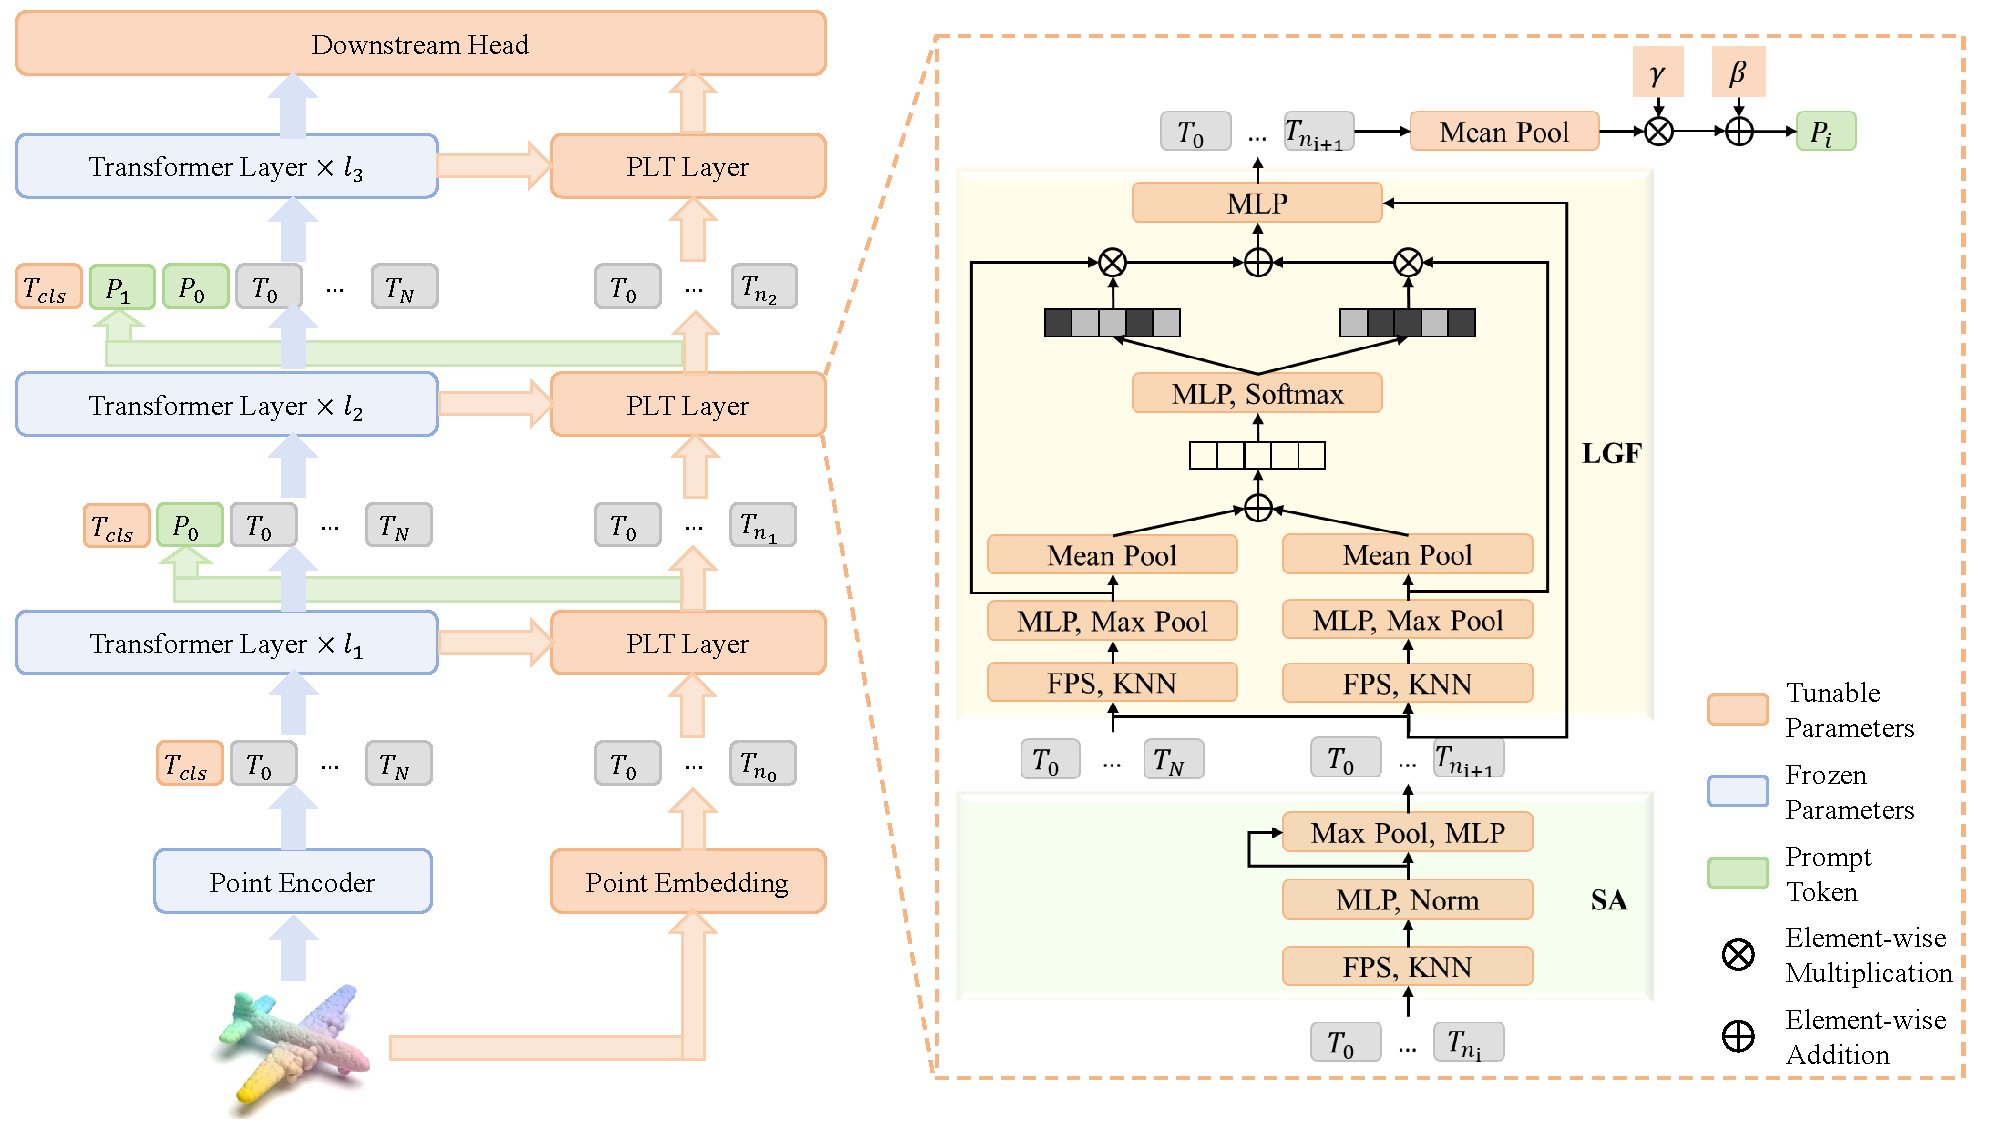
\includegraphics[width=\linewidth]{fig/Overall.pdf}
    \caption{The overall of our PLT. During fine-tuning, we froze the pre-trained backbone network and only fine-tune the PLT branch and the class token. The PLT branch consists of two main components: 1) Set Abstraction (SA), and 2) Local-Global Fusion Module (LGF).
}
    \label{fig:overall}
\end{figure*}

\section{Methodology}
\label{sec:methodology}

To enable effective point cloud fine-tuning of pre-trained models while mitigating the high computational and storage costs associated with full-parameter updates, we propose Point Ladder Tuning (PLT), a parameter-efficient fine-tuning framework for 3D point cloud learning that that integrates hierarchically structured local pathways with dynamic multi-scale prompt guidance. PLT enhances parameter efficiency and task performance by jointly leveraging local geometric details and global semantic cues, thereby overcoming two key limitations: (1) the inability of Ladder Side-Tuning (LST)~\cite{sung2022lst} to effectively capture fine-grained local features, and (2) the limited instance-level adaptability of conventional prompt tuning methods~\cite{li2021prefix}.

As shown in Fig.~\ref{fig:overall2}, the core idea behind PLT is to decouple the fine-tuning process into two synergistic pathways: (1) a lightweight \textbf{Hierarchical Ladder Network (HLN)} that enriches task-specific local geometry modeling(\S\ref{sec:HLN}), and (2) a \textbf{Prompt-based Global Adaption} that dynamically modulates frozen backbone via instance-aware global semantics(\S\ref{sec:FT_backbone}). These pathways are seamlessly integrated through a \textbf{Local-Global Fusion (LGF)} module that enables adaptive, bidirectional information exchange between local and global representations(\S\ref{sec:LGF}).

Finally, we design lightweight, task-specific heads, as detailed in \S\ref{sec:head}. Furthermore, we leverage the hierarchical structure to perform progressive upsampling, which facilitates the recovery of spatial resolution. This design choice proves especially effective for dense prediction tasks, where preserving spatial fidelity is crucial for accurate prediction.

\subsection{Hierarchical Ladder Network}
\label{sec:HLN}

While transformer-based point cloud encoders excel at capturing global semantics, they often struggle with fine-grained spatial understanding due to their limited inductive bias toward local geometric structures. Existing PEFT methods (e.g. PointPEFT~\cite{tang2024point}, PointGST~\cite{liang2024parameter}) attempt to address this by introducing locality-enhancing modules, but still rely heavily on global activations from frozen backbones and typically operate at fixed resolutions, underutilizing the rich local context essential for dense prediction.

To address these limitations, we propose a Hierarchical Ladder Network (HLN) to capture local information across multiple resolutions within the input point cloud. By explicitly modeling multi-scale local features, HLN better aligns with the geometric nature of 3D data and improves performance on tasks such as semantic segmentation. The HLN layer consists of two key components: (1) Set Abstraction (SA) and (2) Local-Global Fusion (LGF) module. In this section, we introduce SA, with LGF discussed further in Sec.~\ref{sec:LGF}.

Given an input point cloud $\mathbf{P} \in \mathbb{R}^{N \times 3}$, where $N$ is the number of points, we first apply point embedding to map $\mathbf{P}$ into a high-dimensional space, resulting in a initial point cloud features $\mathbf{F} \in \mathbb{R}^{N \times C}$, where $C$ represents the feature dimension. We then use Set Abstraction (SA) for downsampling, starting with farthest point sampling (FPS) to select a set of center points $\mathbf{C}=\{c_1, \ldots, c_n\}$, followed by k-Nearest Neighbors (kNN) to define local neighborhoods: 

\begin{equation}
    \mathcal{N}(c_i) = \left\{(\mathbf{p}_{c_i}^j, \mathbf{f}_{c_i}^j) \mid j = 1, \dots, k \right\}.
\end{equation}

The local features are aggregated as:
\begin{align}
    \hat{\mathbf{f}}_{c_i}^{j} &= \varphi\left(\left[\mathbf{f}_{c_i}^{j}; (\mathbf{p}_{c_i} - \mathbf{p}_{c_i}^j)\right]\right), \\
    \mathbf{f}_{c_i}^{\prime} &= \mathbf{f}_{c_i} + \rho\left(h_{\boldsymbol{\Theta}}([\hat{\mathbf{f}}_{c_i}^{1}; \dots; \hat{\mathbf{f}}_{c_i}^{k}])\right),
\end{align}
where $\varphi$, $\rho$ are learnable functions, $h_{\boldsymbol{\Theta}}$ denotes the aggregation function (e.g., max pooling) and $[\cdot ; \cdot]$ denotes concatenation. By stacking multiple SA layers, HLN constructs a hierarchical local representation $\mathbf{F}_l$ that complements global transformer outputs.

\subsection{Local-Global Fusion Module}
\label{sec:LGF}

A key challenge in point cloud representation learning is to effectively integrate fine-grained geometric details with high-level semantic context.. Existing fusion approaches, such as naive concatenation or element-wise addition, typically fail to adaptively balance these two information sources, leading to suboptimal performance, particularly in dense prediction tasks.

To address this issue, we propose a novel Local-Global Fusion (LGF) module that performs adaptive feature integration via selective attention. Our design is motivated by two key insights: (1) local geometric features extracted by the HLN pathway are critical for precise spatial reasoning; and (2) global features from the frozen pre-trained backbone encode rich semantic priors. LGF allows the network to dynamically balance and selectively integrate these complementary representations in a content-aware manner, ensuring that both local details and global semantics are effectively leveraged.

Let $\mathbf{F}_l$ and $\mathbf{F}_g$ denote local and global token features from HLN and the frozen backbone, respectively. we first map the backbone features to match the dimensionality of the HLN layer’s feature vectors using a learnable matrix $W$:

\begin{equation}
	\mathbf{F}_g' = \mathbf{F}_g W
\end{equation}

We then apply an aggregation operation similar to SA without spatial downsampling to capture cross-level interactions. This results in global features $\mathbf{F}_g''$, which model interactions between the local tokens $\mathbf{T}^{L}$ and global tokens $\mathbf{T}^{G}$, while $\mathbf{F}_l$ preserves the intra-local interactions within $\mathbf{T}^{L}$.

To fuse these global and local features, we employ a selective attention mechanism. This mechanism allows the model to focus adaptively on the most relevant information from each feature source, ensuring both global context and local details are integrated effectively. First, we apply an aggregation function $\mathcal{A}$, typically average pooling, to obtain global and local feature descriptors:

\begin{equation}
	\mathbf{f}_l = \mathcal{A}(\mathbf{F}_l), \quad \mathbf{f}_g = \mathcal{A}(\mathbf{F}_g'')
\end{equation}

These local and global descriptors are passed through an MLP to produce attention logits $\mathbf{z}_l$ and $\mathbf{z}_g$:
\begin{equation}
	\mathbf{z}_l, \mathbf{z}_g = \operatorname{split}\left( \alpha \left( \mathbf{f}_l + \mathbf{f}_g \right) \right)
\end{equation}
where $\alpha$ represents an MLP, $\operatorname{split}$ represents the splitting operation along the channel dimension.

We compute soft attention weights for both feature types using a softmax-like formulation:
\begin{equation}
	\mathbf{s}_l^i = \frac{e^{\mathbf{z}_l^i}}{e^{\mathbf{z}_l^i} + e^{\mathbf{z}_g^i}}, \quad
\mathbf{s}_g^i = \frac{e^{\mathbf{z}_g^i}}{e^{\mathbf{z}_l^i} + e^{\mathbf{z}_g^i}}.
\end{equation}

These weights are then used to obtain the fused multi-scale feature representation as a weighted sum:
\begin{equation}
	\mathbf{F}_{ms} = s_l \cdot \mathbf{F}_l + s_g \cdot \mathbf{F}_g''
\end{equation}

Finally, a lightweight MLP $\tau$ is applied to transform the fused features, and a residual connection adds this output to the shortcut features, producing the final fused output:
\begin{equation}
	\mathbf{F}_o = \mathbf{F}_l + \tau(\mathbf{F}_{ms})
\end{equation}

% By dynamically balancing the contributions of local and global representations, the LGF module enables effective integration of fine-grained geometry and high-level semantics. This fusion is especially beneficial for dense prediction tasks, where both local detail and global structure are critical to performance.

\subsection{Dynamic Prompt-Based Tuning}
\label{sec:FT_backbone}
To enable the pre-trained backbone network to produce task-adaptive global representations, we propose a dynamic multi-scale prompt generation strategy driven by the fused feature representation $\mathbf{F}_{o}$ from the LGF module. This design aims to inject instance-specific geometric cues into the transformer backbone, allowing the model to preserve general semantic priors while adapting flexibly to downstream tasks.

Firstly, $F_{o}$ is mean-pooled to obtain a compact representation. This pooled feature is then scaled and shifted using learnable parameters $\gamma$ and $\beta$, generating a multi-scale prompt $\mathbf{p}$. To maximize parameter efficiency, we reuse $W$ from the LGF module to align the dimensionality of the multi-scale prompts with that of the backbone network features. The formula for this process is as follows:
\begin{equation}
	\mathbf{p} = \left(\gamma \cdot \frac{1}{n} \sum_{i=1}^{n} \mathbf{F}_o^i + \beta \right) W^T
\end{equation}
where $n$ is the number of tokens in $F_o$.

Finally, the multi-scale prompts $\mathbf{P}=[\mathbf{p}_{1}, \ldots, \mathbf{p}_{s}]$ are incorporated into the backbone network during training, where $s$ is corresponds to the number of stages in the HLN pathway. These prompts are inserted at each transformer layer of the frozen backbone to condition the global representation in a scale-aware, instance-sensitive manner:
\begin{equation}
	\mathbf{x}_l = \mathcal{L}_l\left([\mathbf{T}_{cls}; \mathbf{P}; \mathbf{T}^{G}]\right)
\end{equation}
where $\mathcal{L}_l$ is the $l$-th transformer layer. 

The injected prompts participate in the attention mechanism, interacting with the original tokens to enrich the contextual modeling without altering the backbone’s architecture. This allows the model to adaptively refine global features based on the special task, while maintaining the semantic richness of large-scale pre-training.

To further enhance adaptability, we adopt the lightweight scale-and-shift tuning strategy proposed in SSF~\cite{lian2022scaling}, applying element-wise affine transformations to the output of each backbone module:

\begin{equation}
	\mathbf{y} = s \cdot \mathbf{x} + t
\end{equation}
where $s$ and $t$ are learnable  scaling and shifting  vectors that fine-tune the global representation with minimal overhead.

Our dynamic prompt-based tuning mechanism combines geometry-aware conditioning with parameter-efficient tuning (PEFT) to enable flexible and effective adaptation to diverse 3D tasks, without requiring task-specific adapters or modifying the backbone. This design significantly increases model expressiveness and task-specific responsiveness, while preserving efficiency and scalability.

\subsection{Downstream Head}
\label{sec:head}

\subsubsection{Classification Head}
For classification tasks, we aggregate local-global cues into a compact descriptor as follows:

\begin{equation}
\mathbf{x}_o = [\mathbf{T}_{cls} + \mathcal{A}_{\text{avg}}(\mathbf{P}); \mathcal{A}_{\text{max}}(\mathbf{T}^{G}); \mathcal{A}_{\text{max}}(\mathbf{T}^{L})]
\end{equation}
where $\mathcal{A}_{\text{avg}}$ and $\mathcal{A}_{\text{max}}$ denote average pooling and max pooling operations, respectively. This aggregated descriptor is then fed into a MLP, followed by a softmax activation to produce the final classification output:
\begin{equation}
\mathbf{y}_{cls} = \operatorname{softmax}(\operatorname{MLP}(\mathbf{x}_o))
\label{eq:MLP}
\end{equation}


\subsubsection{Segmentation Head}
Unlike classification tasks, semantic segmentation requires per-point predictions, necessitating the recovery of features for all original points. A common approach is to propagate features from downsampled representations back to the original point cloud through feature interpolation. However, most existing parameter-efficient fine-tuning methods~\cite{zha2023instance,zhou2024dynamic,liang2024parameter} for point cloud lack the ability to capture multi-resolution information, leading to a considerable loss of local detail.

To address this issue, we introduce an additional HLN branch to extract fine-grained multi-resolution features from the spatial domain. Inspired by PointNext~\cite{qian2022pointnext}, we employ an inverse distance-weighted interpolation strategy to progressively recover the point-level features at each resolution. Different from PointNext~\cite{qian2022pointnext}, we simultaneously leverage both the global features from the backbone and the multi-resolution local features from HLN to upsample. During each interpolation step, these are concatenated to form a comprehensive representation:

\begin{equation}
\mathbf{T}^{\text{interp}} = [\operatorname{Interp}(\mathbf{T}, \mathbf{T}^G); \operatorname{Interp}(\mathbf{T}, \mathbf{T}^L)]
\end{equation}
where $\mathbf{T}$ denotes the point features at the current layer. The function $\operatorname{Interp}(\cdot)$ performs inverse distance interpolation~\cite{qian2022pointnext}.

At each resolution, we concatenate the interpolated features $\mathbf{T}^{\text{interp}}$ with the corresponding original features $\mathbf{T}$, and then pass them through a MLP to obtain updated features. This process is repeated iteratively until the resolution of the original point cloud is restored. Finally, point-wise classification is performed using a MLP followed by a softmax activation, as defined in Eq.~\eqref{eq:MLP}, to predict the semantic category of each point. This design not only enhances segmentation performance but also substantially reduces the number of trainable parameters and overall computational complexity.


\begin{table*}[ht]
    \footnotesize
    \setlength{\tabcolsep}{0.9mm}
    \centering

  \caption{
Classification results on three variants of the ScanObjectNN~\cite{uy2019revisiting} dataset and the ModelNet40~\cite{wu20153d} dataset, including the number of trainable parameters and overall accuracy (OA). All methods apply default data augmentation as used in~\cite{zhou2024dynamic}. \textcolor{red}{$^*$} indicates reproduced results. For ScanObjectNN~\cite{uy2019revisiting}, results are reported without voting. For ModelNet40~\cite{wu20153d}, results are shown without and with voting, respectively denoted as (-/-).
}
  \vspace{-10pt}
    \begin{tabular}{lcccccccc}
    
    \toprule
    \multirow{2.3}{*}{Method} &\multirow{2.3}{*}{Reference} &\multirow{2.3}{*}{Tunable params. (M)} &\multirow{2.3}{*}{FLOPs (G)} &\multicolumn{3}{c}{ScanObjectNN} &\multicolumn{2}{c}{ModelNet40}\\
		\cmidrule(r){5-7} \cmidrule{8-9}
	& & & &OBJ\_BG & OBJ\_ONLY &PB\_T50\_RS & Points Num. & OA (\%)      \\
    \midrule
    \multicolumn{9}{c}{\textit{Supervised Learning Only}} \\
    \midrule
    PointNet~\cite{qi2017pointnet} & CVPR 17 & 3.5 & 0.5  & 73.3  & 79.2  & 68.0 & 1k & - / 89.2 \\
    PointNet++~\cite{qi2017pointnet++}   & NeurIPS 17 & 1.5 & 1.7 & 82.3  & 84.3  & 77.9 & 1k & - / 90.7\\
    DGCNN~\cite{wang2019dynamic}  & TOG 19 & 1.8 & 2.4 & 82.8  & 86.2  & 78.1 & 1k & - / 92.9 \\
    MVTN~\cite{hamdi2021mvtn}  & ICCV 21 & 11.2 & 43.7 & -     & -     & 82.8 & 1k & - / 93.8\\
    PointNeXt~\cite{qian2022pointnext} & NeurIPS 22  & 1.4 & 1.6 & -     & -  & 87.7 & 1k & - / 94.0\\
    PointMLP~\cite{ma2022rethinking}  & ICLR 22 &  13.2 & 31.4  & -    & -     & 85.4  & 1k & - / 94.5\\
    RepSurf-U~\cite{ran2022surface} & CVPR 22 & 1.5   & 0.8 &  -  & -    & 84.3  & 1k  & - / 94.4 \\
    ADS~\cite{hong2023attention} & ICCV 23 & -  & -  &  - & -   & 87.5 & 1k  & - / 95.1 \\
    \midrule
    \multicolumn{9}{c}{\textit{ Self-Supervised Representation Learning (Full fine-tuning)}} \\
    \midrule
    % Transformer~\cite{} &  & 22.1 & & 79.86 & 80.55 &  77.24 & 1k & 91.4 \\
    OcCo~\cite{wang2021unsupervised} & ICCV 21 & 22.1 & 4.8 & 84.85 & 85.54 & 78.79 & 1k & - / 92.1 \\
    Point-BERT~\cite{yu2022point}  & CVPR 22 & 22.1 & 4.8  & 87.43 & 88.12 &  83.07 & 1k & - / 93.2 \\
    MaskPoint~\cite{liu2022masked} & ECCV 22 & 22.1 & - & 89.70 & 89.30 &  84.60 & 1k & - / 93.8 \\
    Point-MAE~\cite{pang2022masked}  & ECCV 22 & 22.1 & 4.8 & 90.02 & 88.29 & 85.18 & 1k & - / 93.8 \\
    Point-M2AE~\cite{zhang2022point}  & NeurIPS 22 & 15.3 & 3.6 & 91.22 & 88.81 & 86.43 
 & 1k & - / 94.0\\
    ACT~\cite{dong2022autoencoders} & ICLR 23 & 22.1 & 4.8 & 93.29 & 91.91  & 88.21 & 1k & - / 93.7\\
    \recon~\cite{qi2023contrast} & ICML 23& 43.6 & 5.3 & 94.15 & 93.12  & 89.73 & 1k & - / 93.9  \\
    
    \midrule
    \multicolumn{9}{c}{\textit{Self-Supervised Representation Learning (Efficient fine-tuning)}} \\
    
    \midrule
    Point-BERT~\cite{yu2022point} (baseline)  & CVPR 22 & 22.1 (100\%) & 4.8 & 87.43 & 88.12 & 83.07& 1k & {92.7} / {\color{gray}{93.2}}\\
    + IDPT~\cite{zha2023instance}& ICCV 23 & 1.7 (7.69\%) & 7.2 & {88.12}\dplus{+0.69} & {88.30}\dplus{+0.18} & {83.69}\dplus{+0.62} &1k & {92.6}{\dtplus{-0.1}} / {\color{gray}{{93.4}}}{\color{gray}{\ddplus{+0.2}}} \\
    + DAPT~\cite{zhou2024dynamic}& CVPR 24 & 1.1 (4.97\%) & 5.0 & {91.05}\dplus{+3.62} & {89.67}\dplus{+1.55} & {85.43}\dplus{+2.36} &1k & {93.1}{\dplus{+0.4}} / {\color{gray}{{93.6}}}{\color{gray}{\ddplus{+0.4}}} \\
    + PointGST~\cite{liang2024parameter}& Arxiv 24 & \textbf{0.6} (\textbf{2.71}\%) & 5.0 & {91.39}\dplus{+3.96} & {89.67}\dplus{+1.55} & {85.64}\dplus{+2.57} &1k & {93.4}{\dplus{+0.7}} / {\color{gray}{{93.8}}}{\color{gray}{\ddplus{+0.6}}} \\
    + LST~\cite{sung2022lst}& NeurIPS 22 & 0.8 (3.38\%) & - & {89.15}\dplus{+2.72} & {89.50}\dplus{+1.38} & {83.17}\dplus{+0.10} &1k & {92.9}{\dplus{+0.2}} / {\color{gray}{{93.3}}}{\color{gray}{\ddplus{+0.1}}} \\
    \rowcolor{linecolor!40}+ PLT ({ours})& - & \textbf{0.6} (\textbf{2.71}\%) & 5.0 & {91.57}\dplus{+4.14} & {89.85}\dplus{+1.73} & {86.09}\dplus{+3.02} &1k & {93.5}{\dplus{+0.8}} / {\color{gray}{{94.2}}}{\color{gray}{\ddplus{+1.0}}} \\
    \midrule
    Point-MAE~\cite{pang2022masked} (baseline)& ECCV 22 & 22.1 (100\%)& 4.8& 90.02 & 88.29 & {85.18} & 1k & 93.2 / {\color{gray}{93.8}}\\
    + IDPT~\cite{zha2023instance}& ICCV 23 & 1.7 (7.69\%) & 7.2 & {91.22}\dplus{+1.20} & {90.02}\dplus{+1.73} & {84.94}\dtplus{-0.24} &1k & {93.3}{\dplus{+0.1}} / {\color{gray}{{94.4}}}{\color{gray}{\ddplus{+0.6}}} \\
    + Point-PEFT\textcolor{red}{$^*$}~\cite{tang2024point}& AAAI 24 & 0.7 (3.13\%) & - & {90.19}\dplus{+0.17} & {89.50}\dplus{+1.21} & {84.35}\dtplus{-0.83} &1k & {94.2}{\dplus{+1.0}} / ~~-~~~~~~~~~~~~\\
   + DAPT~\cite{zhou2024dynamic}& CVPR 24 & 1.1 (4.97\%) & 5.0 & {90.88}\dplus{+0.86} & {90.19}\dplus{+1.90} & {85.08}\dtplus{-0.10} &1k & {93.5}{\dplus{+0.3}} / {\color{gray}{{94.0}}}{\color{gray}{\ddplus{+0.2}}} \\
    + PPT\textcolor{red}{$^*$}~\cite{zhang2024positional}& Arxiv 24 & 1.1 (4.97\%) & 5.0 & {89.50}\dtplus{-0.52} & {89.50}\dplus{+1.21} & {84.91}\dtplus{-0.27} &1k & {93.7}{\dplus{+0.5}} / ~~-~~~~~~~~~~~ \\
    + PointGST\cite{liang2024parameter}& Arxiv 24 & \textbf{0.6} (\textbf{2.71}\%) & 5.0 & {91.74}\dplus{+1.72} & {90.19}\dplus{+1.90} & {85.29}\dplus{+0.11} &1k & {93.5}{\dplus{+0.3}} / {\color{gray}{{94.0}}}{\color{gray}{\ddplus{+0.2}}} \\
    + LST~\cite{sung2022lst}& NeurIPS 22 & 0.8 (3.38\%) & 5.0 & {89.67}\dtplus{-0.35} & {89.67}\dplus{+1.38} & {82.75}\dtplus{-2.43} &1k & {93.2}{\ddplus{+0.0}} / {\color{gray}{{93.8}}}{\color{gray}{\ddplus{+0.0}}} \\
    \rowcolor{linecolor!40}+ PLT ({ours})& - & \textbf{0.6} (\textbf{2.71}\%) & 5.0 & {90.88}\dplus{+0.86} & {90.02}\dplus{+1.73} & {85.46}\dplus{+0.28} &1k & {93.8}{\dplus{+0.6}} / {\color{gray}{{94.0}}}{\color{gray}{\ddplus{+0.2}}} \\
    \bottomrule
    \end{tabular}%
  
      \label{tab:sota}

\end{table*}%


\section{Experiments}
\label{sec:experiments}
%In this section, we conduct an extensive evaluation of the proposed Point Ladder Tuning (PLT) method across multiple point cloud datasets and tasks \lr{add citation for datasets and tasks here}. Our experiments aim to validate the effectiveness of PLT in achieving high performance while maintaining parameter efficiency, comparing it against state-of-the-art methods to highlight its advantages.

%In this section, we present a comprehensive evaluation of the proposed Point Ladder Tuning (PLT) method across diverse point cloud datasets and tasks \lr{cite datasets and tasks here}, and performed our comparison across various downstream tasks as 3D Object Classification, Few-Shot Learning, 3D Dense Prediction Task. The experimental analysis is designed to assess the efficacy of PLT in attaining competitive performance while preserving parameter efficiency.
%Furthermore, we compare PLT against state-of-the-art approaches to demonstrate its superior performance and computational advantages. An ablation study is also included.

In this section, we conduct a comprehensive evaluation of our proposed Point Ladder Tuning (PLT) method across multiple point cloud datasets \lr{cite datasets and tasks here} and diverse tasks, including 3D object classification, few-shot learning, and 3D dense prediction. Our experiments systematically assess PLT's ability to achieve state-of-the-art performance while maintaining parameter efficiency. Through extensive comparisons with existing approaches, we demonstrate PLT's superior performance and computational advantages. Additionally, we present an ablation study to validate the contribution of each key component in our framework.

%\paragraph{Experimental Settings}
To ensure a fair comparison with prior fine-tuning methods~\cite{zha2023instance, zhou2024dynamic}, we maintain identical experimental setups. All experiments were conducted on an NVIDIA GeForce RTX 3090 GPU (24GB) under controlled hardware conditions. During training, we freeze the weights of the pre-trained backbone and fine-tune only a small subset of parameters in the newly introduced modules.

To rigorously evaluate our proposed method, we employ three state-of-the-art pre-trained models as baselines: Point-BERT~\cite{yu2022point}, Point-MAE~\cite{pang2022masked}, and ACT~\cite{dong2022autoencoders}. These models represent diverse pre-training paradigms, ensuring a comprehensive comparison. Detailed discussions of their performance and comparative analysis will be presented in the experiment section.

%To evaluate the effectiveness of our proposed method, we adopt three representative pre-trained models—Point-BERT~\cite{yu2022point}, Point-MAE~\cite{pang2022masked}, and ACT~\cite{dong2022autoencoders}—as baselines. 
%These models cover a diverse set of 3D pre-training paradigms and serve as strong foundations for comparison. 
%Point-BERT~\cite{yu2022point} extends the BERT~\cite{devlin2018bert} framework to 3D point clouds by leveraging a masked point modeling strategy. 
%It learns both low-level geometric structures and high-level semantic features by aligning masked point embeddings with discrete tokens generated by a dVAE-based tokenizer~\cite{vahdat2018dvae}. 
%Point-MAE~\cite{pang2022masked} introduces the masked auto-encoder paradigm into point cloud pre-training, where the model reconstructs masked point patches from the visible ones. 
%This encourages the network to capture meaningful latent representations that generalize well to downstream tasks. 
%To mitigate the challenge of limited labeled 3D data, ACT~\cite{dong2022autoencoders} utilizes a cross-modal teacher-student framework. 
%It transfers knowledge from a fine-tuned cross-modal pre-trained teacher to a 3D point cloud learner, enabling the latter to acquire rich semantic representations through distillation.


\lr{delete or move to corresponding section}
To comprehensively evaluate our proposed method, we select three state-of-the-art pre-trained models as baselines: Point-BERT~\cite{yu2022point}, Point-MAE~\cite{pang2022masked}, and ACT~\cite{dong2022autoencoders}. These models represent diverse 3D pre-training paradigms, providing robust reference points for comparative analysis.
Point-BERT~\cite{yu2022point} adapts the BERT framework~\cite{devlin2018bert} to point cloud processing through masked point modeling. The approach employs a dVAE-based tokenizer~\cite{vahdat2018dvae} to generate discrete tokens, enabling simultaneous learning of geometric structures and semantic features through masked embedding alignment.
Point-MAE~\cite{pang2022masked} implements a masked autoencoder architecture for point cloud pre-training. By reconstructing occluded point patches from visible regions, the model learns transferable latent representations that demonstrate strong generalization across downstream tasks.
To mitigate the challenge of limited labeled 3D data, ACT~\cite{dong2022autoencoders} utilizes a cross-modal teacher-student framework. It transfers knowledge from a fine-tuned cross-modal pre-trained teacher to a 3D point cloud learner, enabling the latter to acquire rich semantic representations through distillation.
%ACT~\cite{dong2022autoencoders} addresses the limited availability of labeled 3D data through a teacher-student learning approach. The method works by first training a "teacher" model on cross-modal knowledge, then transferring this knowledge to a "student" model that works specifically with 3D point clouds. This knowledge transfer helps the 3D model learn better features even with limited point cloud training data.


\subsection{3D Object Classification}
\label{sec:classification}

\textbf{Object Classification on Synthetic Dataset.} We conduct experiments on the ModelNet dataset~\cite{wu20153d}, which contains 12,311 clean 3D CAD models spanning 40 categories. Following the protocol in DAPT~\cite{zhou2024dynamic}, we split ModelNet40 into 9,843 training samples and 2,468 testing samples. During training, we applied standard data augmentation techniques, including random scaling and random translation. The training configuration adheres to the settings used for baseline comparisons. Specifically, the AdamW optimizer is utilized with an initial learning rate of $5 \times 10^{-4}$ and a weight decay of 0.05. A cosine learning rate scheduler with a 10-epoch warm-up period is employed. The model is trained for a total of 300 epochs with a batch size of 32. 

As shown in Tab.~\ref{tab:sota}, without voting, PLT achieves accuracy rates of 93.8\%, 93.5\% and 93.6\% in Point-MAE, Point-BERT and ACT respectively, representing gains of \textbf{0.6\%}, \textbf{0.8\%} and \textbf{0.3 \%} over full fine-tuning. When using voting, PLT continues to outperform full fine-tuning, notably improving Point-BERT’s accuracy by an additional 1.0\%. Compare to other prior arts, our method achieve best performance by fine-tuning Point-BERT, due to \lr{the reason why Point-BERT is best but others is not.}. \lr{add the reason of performance gain here, discuss why there is performance gain.}

\textbf{Object Classification on Real-World Dataset.} While most pre-trained point cloud models are trained on synthetic datasets like ShapeNet~\cite{chang2015shapenet}, which consist of clean, uniformly distributed point clouds, real-world point clouds often present additional challenges such as noise, missing data, and diverse distributions. To evaluate performance in these more realistic scenarios, we use the ScanObjectNN dataset~\cite{uy2019revisiting}, which comprises approximately 15k point cloud samples across 15 categories captured in indoor scenes, often containing background interference and occlusions. The training configuration is consistent with those used for ModelNet~\cite{wu20153d}. As shown in Tab.~\ref{tab:sota}, we evaluate PLT on three variants of the ScanObjectNN dataset (OBJ\_BG, OBJ\_ONLY, and PB\_T50\_RS), using Point-BERT~\cite{yu2022point},  Point-MAE~\cite{pang2022masked} and ACT~\cite{dong2022autoencoders} as baselines.

Our PLT method demonstrates notable accuracy improvements over full fine-tuning in all settings, using only 2.71\% of the parameters. 
Specifically, PLT achieves gains of 4.14\%, 1.73\%, and 3.02\% on the three ScanObjectNN variants with Point-BERT. 
Compared to the state-of-the-art model, PointGST~\cite{liang2024parameter}, PLT achieves accuracy improvements of 0.45\% on Point-BERT~\cite{yu2022point} and 0.17\% on Point-MAE~\cite{pang2022masked} under the most challenging PB\_T50\_RS setting in ScanObjectNN~\cite{uy2019revisiting}, showcasing the robustness and efficiency of our approach in handling real-world noisy and occluded point cloud data. 
Furthermore, PLT exhibits the least performance degradation on the ACT~\cite{dong2022autoencoders} baseline among all point cloud PEFT approaches. 
While other methods suffer from significant accuracy drops, our approach maintains strong performance, underscoring its architectural strength in preserving semantic representations during adaptation. 
Together, these results validate PLT’s superiority in both performance and parameter efficiency in the real scene dataset.

\begin{table}[!t]
  \centering
  \scriptsize
    \setlength{\tabcolsep}{0.7mm}
  \caption{Few-shot learning on ModelNet40\cite{wu20153d}. Overall accuracy (\%)$\pm$the standard deviation (\%) without voting is reported.}
    \begin{tabular}{lccccc}
    \toprule
   \multirow{2.3}{*}{Methods}&\multirow{2.3}{*}{Reference} & \multicolumn{2}{c}{5-way} & \multicolumn{2}{c}{10-way} \\
\cmidrule{3-6}  &        & 10-shot & 20-shot & 10-shot & 20-shot \\
    % \midrule
    % \multicolumn{6}{c}{\textit{with Self-Supervised Representation Learning (Full fine-tuning)}} \\
    % \midrule
    % % OcCo~\cite{wang2021unsupervised} & ICCV 21      & 94.0$\pm$3.6& 95.9$\pm$2.3 & 89.4$\pm$5.1 & 92.4$\pm$4.6 \\
    % % Point-BERT~\cite{yu2022point}  &  CVPR 22    & 94.6$\pm$3.1 & 96.3$\pm$2.7 & 91.0$\pm$5.4 & 92.7$\pm$5.1 \\
    % MaskPoint~\cite{liu2022masked}  &   ECCV 22   & 95.0$\pm$3.7 & 97.2$\pm$1.7 & 91.4$\pm$4.0 & 93.4$\pm$3.5 \\
    % % Point-MAE~\cite{pang2022masked} &   ECCV 22   & 96.3$\pm$2.5 & 97.8$\pm$1.8 & 92.6$\pm$4.1 & 95.0$\pm$3.0 \\
    % Point-M2AE~\cite{zhang2022point} &  NeurIPS 22    & 96.8$\pm$1.8 & 98.3$\pm$1.4 & 92.3$\pm$4.5 & 95.0$\pm$3.0 \\
    % % ACT~\cite{dong2022autoencoders}  & ICLR 23      & 96.8$\pm$2.3 & 98.0$\pm$1.4 & 93.3$\pm$4.0 & 95.6$\pm$2.8 \\
    % VPP~\cite{qi2024vpp} &  NeurIPS 23    & 96.9$\pm$1.9 & 98.3$\pm$1.5 & 93.0$\pm$4.0 & 95.4$\pm$3.1 \\
    % I2P-MAE~\cite{zhang2023learning} &  CVPR 23    & 97.0$\pm$1.8 & 98.3$\pm$1.3 & 92.6$\pm$5.0 & 95.5$\pm$3.0 \\
    % \recon~\cite{qi2023contrast}  & ICML 23      & 97.3$\pm$1.9 & 98.9$\pm$1.2 & 93.3$\pm$3.9 & 95.8$\pm$3.0 \\
    % PointMamba~\cite{liang2024pointmamba} &  NeurIPS 24 & 96.9$\pm$2.0 & 99.0$\pm$1.1 & 93.0$\pm$4.4 & 95.6$\pm$3.2 \\
    % \midrule
    % \multicolumn{6}{c}{\textit{with Self-Supervised Representation Learning (Efficient fine-tuning)}} \\
    \midrule
   Point-BERT~\cite{yu2022point} (baseline) & CVPR 22 &94.6$\pm$3.1 & 96.3$\pm$2.7 & 91.0$\pm$5.4 & 92.7$\pm$5.1 \\
   + IDPT~\cite{zha2023instance} & ICCV 23    & 96.0$\pm$\textbf{1.7}& 97.2$\pm$2.6& 91.9$\pm$4.4& 93.6$\pm$3.5\\
   + DAPT~\cite{zhou2024dynamic} & CVPR 24&95.8$\pm$2.1 &97.3$\pm$1.3 &92.2$\pm$4.3 &94.2$\pm$3.4 \\
   + PointGST~\cite{liang2024parameter}  & Arxiv 24&96.5$\pm$2.4 &97.9$\pm$2.0 &92.7$\pm$4.2 &95.0$\pm$\textbf{2.8} \\
   + LST~\cite{sung2022lst}  & NIPS 22&94.3$\pm$2.6 &97.1$\pm$1.8 &90.6$\pm$4.7 &93.7$\pm$3.7 \\
   \rowcolor{linecolor!40}+ PLT (\textbf{ours}) & -&\textbf{96.9}$\pm$2.0 &\textbf{98.8}$\pm$\textbf{1.1}&\textbf{93.3}$\pm$\textbf{4.0} &\textbf{95.5}$\pm$3.1 \\
    \midrule
    Point-MAE~\cite{pang2022masked} (baseline) &ECCV 22 & 96.3$\pm$2.5 & 97.8$\pm$1.8 & 92.6$\pm$4.1 & 95.0$\pm$3.0\\
   + IDPT~\cite{zha2023instance} &   ICCV 23    & 97.3$\pm$2.1& 97.9$\pm$1.1& 92.8$\pm$4.1& 95.4$\pm$\textbf{2.9}\\
   + DAPT~\cite{zhou2024dynamic} & CVPR 24 & 96.8$\pm$\textbf{1.8}  &  98.0$\pm$1.0 & 93.0$\pm$\textbf{3.5} & \textbf{95.5}$\pm$3.2  \\
   % + PointGST~\cite{liang2024parameter} & Arxiv 24 & \textbf{98.0}$\pm$\textbf{1.8}  &  98.3$\pm$\textbf{0.9} & \textbf{93.7}$\pm$\textbf{4.0} & \textbf{95.7}$\pm$\textbf{2.4}  \\
   + LST~\cite{sung2022lst}  & NIPS 22&96.6$\pm$2.5 &97.5$\pm$1.7 &92.0$\pm$4.4 &94.9$\pm$3.2 \\
   \rowcolor{linecolor!40}+ PLT (\textbf{ours}) & - & \textbf{97.2}$\pm$2.2  &  \textbf{98.9}$\pm$\textbf{0.9} & \textbf{93.2}$\pm$4.2 & \textbf{95.5}$\pm$\textbf{2.9}  \\
   \midrule
   ACT~\cite{dong2022autoencoders} (baseline) & ICLR 23 & 96.8$\pm$2.3 & 98.0$\pm$1.4 & 93.3$\pm$4.0 & 95.6$\pm$2.8\\
   + IDPT~\cite{zha2023instance} &   ICCV 23    & 96.8$\pm$1.9& 98.3$\pm$1.2& 92.5$\pm$4.1& 95.3$\pm$3.3\\
   + DAPT~\cite{zhou2024dynamic} & CVPR 24 & 95.3$\pm$2.8  &  97.1$\pm$1.7 & 89.8$\pm$4.8 & 94.1$\pm$3.6  \\
   + PPT~\cite{zhang2024positional}  & Arxiv 24 & \textbf{97.1}$\pm$2.3 &98.1$\pm$1.8 &91.8$\pm$4.3 &94.9$\pm$3.4 \\
   + PointGST~\cite{liang2024parameter} & Arxiv 24 & 97.2$\pm$1.9  &  98.3$\pm$1.3 & 92.9$\pm$4.2 & 95.7$\pm$\textbf{2.6}  \\
   + LST~\cite{sung2022lst}  & NIPS 22&96.2$\pm$2.6 &98.0$\pm$1.9 &92.6$\pm$4.4 &94.9$\pm$3.4 \\
   \rowcolor{linecolor!40}+ PLT (\textbf{ours}) & - & 96.9$\pm$\textbf{1.8}  &  \textbf{98.9}$\pm$\textbf{1.0} & \textbf{93.4}$\pm$\textbf{4.0} & \textbf{95.9}$\pm$3.1  \\
    \bottomrule
    % \vspace{-12pt}
    \end{tabular}%
  \label{tab:fewshot}%
\end{table}%

\subsection{Few-Shot Learning}
\label{sec:few_shot}

We further evaluate the transferability of PLT in a few-shot learning setting using the ModelNet40~\cite{wu20153d} dataset, which serves as a standard benchmark for assessing the efficiency of data usage in low-resource settings. The training configuration follows that of the 3D object classification task, with the exception that the number of training epochs is set to 150. Following prior works~\cite{zha2023instance, zhou2024dynamic}, we adopt the standard n-way m-shot protocol, where $n \in \{5, 10\}$ and $m \in \{10, 20\}$.

As summarized in Tab.~\ref{tab:fewshot}, our PLT consistently outperforms both full fine-tuning and state-of-the-art PEFT methods across the majority of settings, regardless of the choice of pre-trained backbone (Point-BERT~\cite{yu2022point}, Point-MAE~\cite{pang2022masked}, or ACT~\cite{dong2022autoencoders}). For example, under the 5-way 20-shot setting, our PLT achieves a overall accuracy of 98.8\% with Point-BERT~\cite{yu2022point}, outperforming other methods such as full fine-tuning (+2.5\%) and PointGST~\cite{liang2024parameter} (+0.9\%). These results highlight our PLT's strong capability to generalize under data-scarce conditions and validate its effectiveness in few-shot point cloud learning tasks.

In addition to superior accuracy, our PLT also demonstrates improved stability across few-shot settings. As shown in Tab.~\ref{tab:fewshot}, our method yields consistently lower or comparable standard deviations compared to other PEFT baselines. For instance, under the 5-way 20-shot setting, PLT achieves a standard deviation of only $\pm$1.1\% with Point-BERT, outperforming other methods such as LST~\cite{sung2022lst} ($\pm$1.8\%) and PointGST~\cite{liang2024parameter} ($\pm$2.0\%). This trend is observed across multiple configurations, indicating that PLT not only improves mean performance but also reduces performance variance across different folds. Such stability is particularly critical in few-shot learning scenarios, where training data is limited and model robustness becomes more important.

\subsection{Comparison with Cross-domain PEFT Methods}
\label{sec:compare}

We compare our PLT with a broad range of PEFT methods originally proposed for NLP and 2D vision, adapting them to point cloud scenarios. As shown in Tab.~\ref{tab:origin_finetuning}, methods like VPT~\cite{jia2022visual} and Adapter~\cite{houlsby2019parameter} suffer significant accuracy drops when transferred to the 3D domain. For example, VPT~\cite{jia2022visual} leads to a 4.09\% decrease on the challenging PB\_T50\_RS variant compared to full fine-tuning. Similarly, although Adapter~\cite{houlsby2019parameter} achieves moderate gains on OBJ\_ONLY, it performs poorly on more complex tasks.

LST~\cite{sung2022lst} provides competitive performance in specific settings, but its generalization across variants is limited. In contrast, PLT achieves consistently strong results across various challenging scenarios, while tuning only 0.6M parameters, a fraction of the full model size.

Further comparisons in Tab.~\ref{tab:compare} highlight PLT’s superiority under parameter-efficient fine-tuning (PEFT) settings. It outperforms all other PEFT methods, including the strongest 3D-specific methods like PointGST~\cite{liang2024parameter} and DAPT~\cite{zhou2024dynamic}, especially on the most difficult variant PB\_T50\_RS.

These results reveal that many PEFT approaches from other domains struggle with 3D data due to domain gaps and architectural mismatches. Even recent 3D-specific methods face challenges in balancing accuracy and parameter efficiency. In contrast, PLT offers robust generalization, lightweight adaptation, and state-of-the-art performance, establishing itself as a unified and effective PEFT solution for 3D point cloud classification.

\begin{table}
\scriptsize
\setlength{\tabcolsep}{1.9mm}
\centering
\caption{Comparisons of parameter efficient transfer learning methods from NLP and 2D Vision on the hardest variant of ScanObjectNN~\cite{uy2019revisiting}. Overall accuracy (\%) without voting is reported. \#TP represents the tunable parameters. \textcolor{red}{$^*$} denotes reproduced results.}
\label{tab:compare}
\begin{tabular}{ lcccc }
\toprule
 Method &Reference& Design for &\#TP (M) & PB\_T50\_RS \\
\midrule
 Point-MAE~\cite{pang2022masked}  &ECCV 22 & - & 22.1 & 85.18  \\
 Linear probing &- & - & 0.3& 75.99\\
 \midrule
  + Adapter~\cite{houlsby2019parameter}&ICML 19 & NLP & 0.9 & 83.93 \\
  + Perfix tuning~\cite{li2021prefix}& ACL 21 & NLP &0.7 & 77.72  \\
  + BitFit~\cite{zaken2022bitfit} & ACL 21 & NLP &0.3 & 82.62    \\
  + LST~\cite{sung2022lst} & NeurIPS 22 & NLP & 0.8 & 82.75\\
  + LoRA~\cite{hu2021lora} & ICLR 22 & NLP & 0.9&  81.74   \\
  % + DEPT~\cite{shi2024dept} & ICLR 24 & NLP & 0.3 & 79.70\\
  + FourierFT~\cite{Gao2024Fourier} & ICML 24 & NLP &0.3 & 78.57\\
  \midrule
  + VPT-Deep~\cite{jia2022visual}&ECCV 22 & 2D &0.4 &  81.09 \\
  + AdaptFormer~\cite{chen2022adaptformer} &NeurIPS 22 & 2D &0.9  & 83.45 \\
  + SSF~\cite{lian2022scaling} & NeurIPS 22 & 2D &0.4  & 82.58\\
  + FacT~\cite{jie2023fact} & AAAI 23 & 2D & 0.5 & 78.76\\
  % + BI-AdaptFormer~\cite{jie2023revisiting} & ICCV 23 & 2D & 0.4 & 83.66\\
  + SCT~\cite{zhao2024sct} & IJCV 24 & 2D & 0.3 & 80.40\\
  \midrule
  + IDPT~\cite{zha2023instance} &ICCV 23 & 3D & 1.7 &84.94\\
  + Point-PEFT\textcolor{red}{$^*$}~\cite{tang2024point} & AAAI 24 & 3D & 0.7 &84.35\\
  + DAPT~\cite{zhou2024dynamic} & CVPR 24 & 3D & 1.1 & 85.08 \\
  + PPT\textcolor{red}{$^*$}~\cite{zhang2024positional} & Arxiv 24 & 3D & 1.1 & 84.91\\
  + PointGST~\cite{liang2024parameter} & Arxiv 24 & 3D & 0.6 & 85.29\\
  % + PointLoRA~\cite{wang2025pointlora} & CVPR 25 & 3D & 0.8 & \textbf{85.53}\\
  \rowcolor{linecolor!40}+ PLT (\textbf{ours}) & - & 3D & 0.6 & \textbf{85.53} \\
\bottomrule
\end{tabular}
\end{table}


\begin{table}
\footnotesize
\setlength{\tabcolsep}{1.6mm}
\centering
\caption{The overall accuracy (\%) for classical fine-tuning strategies on three variants of ScanObjectNN~\cite{uy2019revisiting} is reported. `\#TP’ means the number of tunable parameters. Linear probing indicates head-tuned only.}
\label{tab:origin_finetuning}
\begin{tabular}{ lcccc }
\toprule
Tuning Strategy & \#TP(M) &OBJ\_BG &OBJ\_ONLY & PB\_T50\_RS \\
\midrule
Point-MAE~\cite{pang2022masked} & 22.1 & 90.02 & 88.29 & 85.18 \\
Linear probing & 0.3  & 87.26\dtplus{-2.76} & 84.85\dtplus{-3.44} & 75.99\dtplus{-9.19}\\
\midrule
+ Adapter~\cite{houlsby2019parameter} & 0.9  & 89.50\dtplus{-0.52} & 88.64\dplus{+0.35} & 83.93\dtplus{-1.25}\\
+ VPT~\cite{jia2022visual} & 0.4  & 87.26\dtplus{-2.76} & 87.09\dtplus{-1.20} &81.09\dtplus{-4.09} \\
+ LST~\cite{sung2022lst} & 0.8  & 89.67\dtplus{-0.25} & 89.67\dplus{+1.38} &82.75\dtplus{-2.43} \\
\bottomrule
\end{tabular}
\end{table}

\subsection{3D Dense Prediction Task}
For dense prediction tasks, including part segmentation and semantic segmentation, we adopt a prediction head similar to that of PointNext~\cite{qian2022pointnext}, allowing us to effectively utilize multi-resolution information and enhance performance while maintaining a low number of trainable parameters.

We validate the effectiveness of PLT on the ShapeNetPart dataset~\cite{yi2016scalable}, comprising 16,881 samples distributed across 16 object categories and 50 part categories. Training is performed using the AdamW optimizer with a weight decay of 0.05 and a cosine learning rate scheduler. The initial learning rate is set to $2 \times 10^{-4}$, with a warm-up period of 10 epochs. The models are trained for 300 epochs using a batch size of 16. As shown in Tab.~\ref{tab:segmentation}, PLT achieves results comparable to other methods in terms of instance-level mIoU (Inst. mIoU) while achieving notable improvements in class-level mIoU (Cls. mIoU). Specifically, PLT improves Inst. mIoU on PointBERT~\cite{yu2022point} by 0.5\% over DAPT~\cite{zhou2024dynamic}, demonstrating its effectiveness in capturing fine-grained details.

\begin{table}
  \centering
  \scriptsize
  \setlength{\tabcolsep}{0.6mm}
  \caption{Part segmentation on the ShapeNetPart~\cite{yi2016scalable}. The mIoU for all classes (Cls.) and for all instances (Inst.) are reported. \#TP represents the tunable parameters. \textcolor{red}{$^*$} denotes reproduced results.}
    \vspace{-10pt}
    \begin{tabular}{lcccc}
    \toprule
    Methods & Reference & \#TP (M)& Cls. mIoU (\%) & Inst. mIoU (\%) \\
    \midrule
    \multicolumn{5}{c}{\textit{Supervised Learning Only}} \\
    \midrule
    PointNet~\cite{qi2017pointnet}  & CVPR 17  &- & 80.39 & 83.7 \\
    PointNet++~\cite{qi2017pointnet++}    & NeurIPS 17 &-  & 81.85 & 85.1 \\
    DGCNN~\cite{wang2019dynamic}  & TOG 19 & - & 82.33 & 85.2 \\
    APES~\cite{wu2023attention} & CVPR 23& - & 83.67 & 85.8\\
    \midrule
    \multicolumn{5}{c}{\textit{ Self-Supervised Representation Learning (Full fine-tuning)}} \\
    \midrule
    % Transformer \cite{} & & 27.09 & 83.42 & 85.1 \\
    OcCo~\cite{wang2021unsupervised}  & ICCV 21 & 27.09 & 83.42 & 85.1 \\
    MaskPoint~\cite{liu2022masked}  & ECCV 22 & - & 84.60 & 86.0 \\
    Point-BERT~\cite{yu2022point}  & CVPR 22 & 27.09 & 84.11 & 85.6 \\
    Point-MAE~\cite{pang2022masked}  & ECCV 22 & 27.06 & 84.19 & 86.1 \\ 
    ACT~\cite{dong2022autoencoders}  & ICLR 23 &  27.06 & 84.66 & 86.1 \\
    \midrule
    \multicolumn{5}{c}{\textit{ Self-Supervised Representation Learning (Efficient fine-tuning)}} \\
    \midrule
    Point-BERT~\cite{yu2022point} (baseline) &  CVPR 22 & 27.09 & 84.11 & 85.6 \\ 
    + IDPT\textcolor{red}{$^*$}~\cite{zha2023instance} & ICCV 23 & 5.69  & 83.50  & 85.3  \\
    + DAPT~\cite{zhou2024dynamic} & CVPR 24 & 5.65  & 83.83 & 85.5 \\
    % + PointGST~\cite{liang2024parameter} & Arxiv 24 & 5.58  & \textbf{83.87} & 85.7 \\
    \rowcolor{linecolor!40}+ PLT (\textbf{ours})& - & \textbf{2.08}  & \textbf{83.85} & \textbf{86.0} \\
    \midrule
    Point-MAE~\cite{pang2022masked} (baseline) &  ECCV 22 & 27.06 & 84.19 & 86.1 \\ 
    + IDPT~\cite{zha2023instance} & ICCV 23 & 5.69  & 83.79  & 85.7  \\
    + DAPT~\cite{zhou2024dynamic} & CVPR 24 & 5.65  & 84.01 & 85.7 \\
    % + PPT~\cite{zhang2024positional} & Arxiv 24 & 5.62  & \textbf{84.07} & 85.7 \\
    % + PointGST~\cite{liang2024parameter} & Arxiv 24 & 5.59  & 83.98 & 85.8 \\
    \rowcolor{linecolor!40}+ PLT (\textbf{ours})& - & \textbf{2.08}  & 83.90 & \textbf{85.9} \\
    \bottomrule
    \end{tabular}
    % \vspace{-10pt}
  \label{tab:segmentation}
\end{table}

To comprehensively evaluate the effectiveness of our proposed PLT framework on dense prediction tasks, we conduct semantic segmentation experiments on two widely adopted large-scale indoor scene datasets: S3DIS~\cite{armeni20163d}and ScanNetV2~\cite{dai2017scannet}, with results summarized in Tab.~\ref{tab:semantic_segmentation}. 

S3DIS~\cite{armeni20163d} is a large-scale indoor scene dataset comprising six areas with a total of 273 million points annotated across 13 categories. Following established practices~\cite{dong2022autoencoders}, Area 5 is recommended for evaluation to provide a more reliable and standardized assessment of performance in semantic segmentation tasks. The model is trained using a cosine learning rate scheduler with an initial learning rate of $2 \times 10^{-4}$. Training is performed over 60 epochs with a batch size of 32, while other configurations are consistent with those used for ShapeNetPart~\cite{yi2016scalable}.

ScanNetV2~\cite{dai2017scannet}is a large-scale benchmark dataset for indoor 3D scene understanding, encompassing a diverse range of environments, from compact residential and office spaces to expansive public and commercial buildings. The dataset comprises 1,513 RGB-D scanned scenes with annotations for 20 semantic categories. Following standard practice, 1,201 scenes are used for training and 312 scenes for testing.For training, we adopt a cosine annealing learning rate scheduler, with an initial learning rate set to $5 \times 10^{-3}$. The models are trained for 500 epochs using a batch size of 32.

As reported in Tab.~\ref{tab:semantic_segmentation}, PLT consistently achieves superior performance across all baselines and datasets, while maintaining a significantly lower number of tunable parameters (2.04M) compared to full fine-tuning (27.02M for Point-MAE~\cite{pang2022masked}, for example). On S3DIS~\cite{armeni20163d}, PLT outperforms all PEFT competitors under each backbone. When applied to ACT~\cite{dong2022autoencoders} as the backbone, PLT achieves an mAcc of 70.6\% and mIoU of 61.5\%, improving over the closest competitor PPT~\cite{zhang2024positional} by 2.3\% in mIoU. Similar trends are observed for Point-MAE~\cite{pang2022masked} and Point-BERT~\cite{yu2022point}, with PLT consistently pushing mIoU to above 61\%, outperforming alternatives such as IDPT~\cite{zha2023instance}, DAPT~\cite{zhou2024dynamic}, and PointGST~\cite{liang2024parameter}.

On the more complex ScanNetV2 dataset~\cite{dai2017scannet}, which demands strong generalization due to its large-scale and real-world variability, PLT again demonstrates robust performance. With the Point-BERT~\cite{yu2022point} backbone, PLT reaches a voxel mIoU (VmIoU) of 48.2\% and point mIoU (PmIoU) of 47.8\%, leading the field in both metrics. Notably, the performance gap between PLT and existing methods becomes more evident here: PLT surpasses DAPT~\cite{zhou2024dynamic} and PointGST~\cite{liang2024parameter} by 4.6\% and 1.9\% respectively on VmIoU, further underscoring its strong adaptability in real-world 3D segmentation scenarios.

These results reinforce the effectiveness of PLT as a lightweight and generalizable PEFT framework for 3D semantic segmentation. Compared with recent 3D-specific PEFT methods (e.g., PointGST~\cite{liang2024parameter}, DAPT~\cite{zhou2024dynamic}), PLT delivers consistent improvements across multiple backbones and datasets, achieving higher accuracy with fewer trainable parameters. Its strong performance on both S3DIS~\cite{armeni20163d} and ScanNetV2~\cite{dai2017scannet} highlights PLT’s ability to retain dense spatial and global contextual information, making it particularly well-suited for challenging 3D scene dense prediction tasks.

\begin{table}
  \centering
  \scriptsize
  \setlength{\tabcolsep}{1.2mm}
  \caption{Semantic segmentation on the S3DIS~\cite{armeni20163d} and ScanNetV2~\cite{dai2017scannet}. The
    mean accuracy (mAcc) and mean IoU (mIoU) are reported on the S3DIS. VmIoU and PmIoU represents Voxel mIoU and Point mIoU respectively.
    \#TP represents the tunable parameters.}
    \begin{tabular}{lcccccc}
    \toprule
    Methods & Reference & \#TP (M)& \multicolumn{2}{c}{S3DIS} & \multicolumn{2}{c}{ScanNetV2} \\
    & & & mAcc & mIoU & VmIoU & PmIoU \\
    \midrule
    Point-BERT~\cite{yu2022point} (baseline) &  CVPR 22 & 27.02 & 69.7 & 62.1 & 49.9 & 49.6 \\ 
    + Linear probing & - & 5.20  & 65.9  & 56.0 & 30.3 & 30.1  \\
    + IDPT~\cite{zha2023instance} & ICCV 23 & 5.64  & 66.9  & 57.7 & 33.9 & 33.6  \\
    + DAPT~\cite{zhou2024dynamic} & CVPR 24 & 5.61  & 68.3 & 58.9 & 43.6 & 43.3 \\
    + PPT~\cite{zhang2024positional} & Arxiv 24 & 5.58 & 68.8 & 60.5 & 46.7 & 46.3 \\
    + PointGST~\cite{liang2024parameter} & Arxiv 24 & 5.55  & 68.5 & 59.5 & 46.3 & 45.8  \\
    + LST~\cite{sung2022lst} & NeurIPS 22 & 5.65 & 67.4 & 58.6 & 34.5 & 34.2  \\
    \rowcolor{linecolor!40}+ PLT (\textbf{ours})& - & \textbf{2.04}  & \textbf{69.6} & \textbf{61.1} & \textbf{48.2} & \textbf{47.8}  \\
    \midrule
    Point-MAE~\cite{pang2022masked} (baseline) &  ECCV 22 & 27.02 & 69.9 & 60.8 & 51.2 & 50.8 \\ 
    + Linear probing & - & 5.20  & 63.4  & 52.5 & 30.9 & 30.7 \\
    + IDPT~\cite{zha2023instance} & ICCV 23 & 5.64  & 66.6  & 57.6 & 33.5 & 33.2  \\
    + Point-PEFT~\cite{tang2024point} & ICCV 23 & 5.58  & 66.5  & 56.0 & - & -  \\
    + DAPT~\cite{zhou2024dynamic} & CVPR 24 & 5.61  & 68.2 & 59.3 & 41.1 & 40.7 \\
    + PPT~\cite{zhang2024positional} & Arxiv 24 & 5.58 & 68.7 & 60.4 & 46.2 & 45.8\\
    + PointGST~\cite{liang2024parameter} & Arxiv 24 & 5.55  & 68.4 & 58.6 & 44.6 & 44.2\\
    + LST~\cite{sung2022lst} & NeurIPS 22 & 5.65 & 66.9 & 57.7 & 35.2 & 34.9 \\
    \rowcolor{linecolor!40}+ PLT (\textbf{ours})& - & \textbf{2.04}  & \textbf{70.5} & \textbf{61.5} & \textbf{47.2} & \textbf{46.8} \\
    \midrule
    ACT~\cite{dong2022autoencoders} (baseline) &  ICLR 23 & 27.02 & 71.1 & 61.2 & 50.9 & 50.5 \\ 
    + Linear probing & - & 5.20  & 64.1  & 52.0 & 27.2 & 27.0 \\
    + IDPT~\cite{zha2023instance} & ICCV 23 & 5.64  & 64.9  & 55.2 & 32.1 & 31.9 \\
    + Point-PEFT~\cite{tang2024point} & ICCV 23 & 5.58  & 66.0  & 54.6 & - & - \\
    + DAPT~\cite{zhou2024dynamic} & CVPR 24 & 5.61  & 67.9 & 58.5 & 40.3 & 40.0 \\
    + PPT~\cite{zhang2024positional} & Arxiv 24 & 5.58 & 69.1 & 59.2 & 45.5 & 45.2\\
    + PointGST~\cite{liang2024parameter} & Arxiv 24 & 5.55  & 67.6 & 57.4 & 44.2 & 43.8 \\
    + LST~\cite{sung2022lst} & NeurIPS 22 & 5.65 & 67.6 & 58.3 & 34.0 & 33.7 \\
    \rowcolor{linecolor!40}+ PLT (\textbf{ours})& - & \textbf{2.04}  & \textbf{70.6} & \textbf{61.5} & \textbf{46.9} & \textbf{46.6} \\
    \bottomrule
    \end{tabular}
  \label{tab:semantic_segmentation}
\end{table}


\begin{table}[!t]
\scriptsize
\setlength{\tabcolsep}{4.5mm}
\centering
 % \footnotesize
\caption{The effect of each component of our LST. SSF and DP represent Scale\&Shift Fine-tuning and Dynamic Prompt respectively. The tunable parameters (\#TP) and the overall accuracy (\%) on the hardest variant of ScanObjectNN\cite{uy2019revisiting} are reported.}
\label{tab:part}

\begin{tabular}{ ccccc }
   \toprule
 SSF & DP & HLN &  \#TP (M) & PB\_T50\_RS \\
\midrule
\multicolumn{3}{c}{Full fine-tuning}  &22.1 & 85.18 \\
\multicolumn{3}{c}{Linear Probing}  &0.27 & 75.99 \\
\midrule
&\ding {52} &\ding {52}& 0.49 & 84.52 \\
\ding {52}  & &\ding {52}& 0.60 &84.66 \\
\ding {52}  & & & 0.37 & 83.34\\
\rowcolor{linecolor!40}\ding {52}  &\ding {52} &\ding {52}  & 0.60 & \textbf{85.53} \\
\bottomrule
\end{tabular}
\end{table}

\begin{table*}
    \centering
    \scriptsize
    \caption{Ablation on hyper-parameters and settings of LST, including the num of neighbors $K$, feature dim $d$ and the num of layers in Hierarchical Ladder Network (HLN). The tunable parameters (\#TP) and the overall accuracy (\%) on the hardest variant of ScanObjectNN\cite{uy2019revisiting} are reported.}
    \label{tab:ablation}
      \vspace{-5pt}
    \resizebox{0.95\linewidth}{!}{
    \begin{subtable}[t]{0.25\linewidth} % 0.245
        \centering
        \scriptsize
         \setlength{\tabcolsep}{1.2mm} % 1.2mm
        \caption{Ablation on $K$ in HLN.}
        \label{tab:k}
        \begin{tabular}{ccc}
           \toprule
            $K$ & \#TP (M) & PB\_T50\_RS \\
            \midrule
            \text{[16, 16, 16]} & 0.60 & 84.46 \\
            \text{[4, 4, 4]} & 0.60 & 84.66 \\
            \text{[4, 8, 16]} & 0.60 & 84.91 \\
            \rowcolor{linecolor!40} \text{[16, 8, 4]} & 0.60 & \textbf{85.46} \\
            \bottomrule
        \end{tabular}
    \end{subtable}

    \begin{subtable}[t]{0.4\linewidth} % 0.235
        \centering
        \scriptsize
         \setlength{\tabcolsep}{1.2mm} % 0.2mm
        \caption{Ablation on $d$ in HLN.}
        \label{tab:dim}
        \begin{tabular}{ccc}
            \toprule
            Feature Dim & \#TP (M) & PB\_T50\_RS \\
            \midrule
            \text{[8, 16, 32, 64]} & 0.46 & 83.17 \\
            \rowcolor{linecolor!40} \text{[16, 32, 64, 128]} & 0.60 & \textbf{85.46} \\
            \text{[32, 64, 128, 256]} & 1.00 & 84.25 \\
            \bottomrule
        \end{tabular}
    \end{subtable}

    \begin{subtable}[t]{0.24\linewidth} % 0.22
    \setlength{\tabcolsep}{1.0mm} % 1.3mm
        \centering
         \scriptsize
        \caption{Ablation on the num of layers.}
        \label{tab:layer}
     
        \begin{tabularx}{\textwidth}{ccc}
            \toprule
            Layer num & \#TP (M) & PB\_T50\_RS \\
            \midrule
            1 & 0.40 & 83.55 \\
            2 & 0.45 & 84.84 \\
            \rowcolor{linecolor!40}3 & 0.60 & \textbf{85.46} \\
            4 & 1.09 & 85.05 \\
            \bottomrule
        \end{tabularx}
    \end{subtable}
}
% \vspace{-10pt}
\end{table*}

\begin{table}[!t]
\scriptsize
\setlength{\tabcolsep}{7.3mm}
\centering
\caption{Fusion way for local and global information in point clouds. The tunable parameters (\#TP) and the overall accuracy (\%) on the hardest variant of ScanObjectNN\cite{uy2019revisiting} are reported.}
\vspace{-10pt}
\label{tab:fusion_way}

\begin{tabular}{ccc}
\toprule
Fusion Way & \#TP (M) & PB\_T50\_RS \\
\midrule
Add & 0.58 & 85.01 \\
Concat & 0.62 & 84.63 \\
Only Global & 0.56 & 84.52 \\
Only Local & 0.56 & 82.86 \\
LGA with Sigmoid & 0.59 & 84.59 \\
\rowcolor{linecolor!40}LGA with Softmax & 0.60 & \textbf{85.46} \\
\bottomrule
\end{tabular}
% \vspace{-10pt}
\end{table}


\begin{table}[!t]
\scriptsize
\setlength{\tabcolsep}{7.8mm}
\centering
\caption{Comparison between HLN and PLT. The tunable parameters (\#TP) and the overall accuracy (\%) on the hardest variant of ScanObjectNN are reported. }
\vspace{-10pt}
\label{tab:sidenet}

\begin{tabular}{ccc}
\toprule
Method & \#TP (M) & PB\_T50\_RS \\
\midrule
Point-MAE & 22.1 & 85.18 \\
% Linear probing & 0.3 & 75.99 \\
HLN & 0.2 & 80.74 \\
\rowcolor{linecolor!40} PLT(Ours) & 0.6 & \textbf{85.46} \\
\bottomrule
\end{tabular}
% \vspace{-15pt}
\end{table}


\subsection{Ablation Study}

\textbf{Effectiveness of PLT Components}. We first investigate the contribution of each individual module in PLT through controlled ablation studies. As shown in Table VII, removing any of the three core components—Scale \& Shift Fine-tuning (SSF), Dynamic Prompting (DP), or the Hierarchical Ladder Network (HLN)—leads to a notable drop in accuracy on the most challenging ScanObjectNN variant (PB\_T50\_RS). As shown in Tab.~\ref{tab:part}, excluding HLN results in a performance decline from 85.53\% to 83.34\%, while excluding SSF or DP alone reduces accuracy to 84.52\% and 84.66\%, respectively. These results clearly demonstrate the complementary roles of all three modules, highlighting that the full integration of SSF, DP, and HLN is essential for maximizing transferability and performance efficiency.

\textbf{Hyperparameter Ablation for Hierarchical Ladder Network.} We conduct a detailed ablation study on the hyperparameters of the HLN, including the number of nearest neighbors $K$, feature dimensions $d$, and the number of hierarchical layers. As summarized in Tab.\ref{tab:ablation}, performance peaks when using $K=[16,8,4]$, feature dimensions $d=[16,32,64,128]$, and a 3-layer architecture, achieving an accuracy of 85.53\% with only 0.60M tunable parameters. This design follows an intuitive hierarchical principle: as the depth of the network increases, the point cloud is progressively downsampled, leading to a reduced number of points in deeper layers. Correspondingly, the number of nearest neighbors $K$ is decreased layer by layer to ensure that neighborhood aggregation remains local and meaningful. If a large $K$ were retained in deeper layers, the receptive field would become overly large relative to the reduced spatial resolution, potentially diluting fine-grained local cues and introducing noise from unrelated distant points. By contrast, using a decreasing neighbor size—such as $K=[16,8,4]$—strikes a balance between capturing sufficient local context in shallow layers and preserving locality in deeper layers. This adaptive design improves the model’s ability to learn multi-scale features across hierarchical levels, leading to superior performance in downstream tasks.

\textbf{Comparison Between HLN and PLT.} To further quantify the value of HLN and its integration within PLT, we compare their standalone performances in Tab.\ref{tab:sidenet}. While HLN alone achieves 80.74\%, integrating it into the full PLT framework improves accuracy to 85.53\%, outperforming even full fine-tuning (85.18\%) with less than 3\% of the tunable parameters. This underscores the importance of coupling lightweight local reasoning structures like HLN with pretrained global backbones for optimal performance.

\textbf{Fusion Strategy for Local and Global Information.} The integration strategy of local and global information plays a critical role in downstream performance. In Tab.~\ref{tab:fusion_way}, we evaluate several fusion mechanisms. The proposed Local-Global Fusion (LGF) with Softmax achieves the highest accuracy (85.53\%), outperforming additive, concatenative, and single-source approaches. Notably, leveraging only local features yields a considerably lower accuracy (82.86\%) than relying solely on global features (84.52\%), reflecting the benefits of pretraining on global representation learning.

\textbf{Attention Score of LGF}. To gain deeper insight into the behavior of LGF, we visualize the local attention weights $s_l$ across categories and network layers in Fig.~\ref{fig:attention_score}. The results reveal three key patterns:

\begin{enumerate}
    \item The local attention scores are generally lower than 0.5, reaffirming the reliance on pretrained global priors.
    \item Category-specific variation is more pronounced in early layers and becomes increasingly uniform in deeper layers, suggesting a hierarchical fusion where shallow layers capture category-aware local details while deeper layers consolidate generalized global semantics.
    \item A downward trend in attention to local features from the first to third layers further supports the notion that the network progressively shifts focus from fine-grained local patterns to more abstract global concepts.
\end{enumerate}

These findings collectively validate the design of PLT as a lightweight yet powerful PEFT framework for 3D transfer learning, wherein carefully balanced architectural and fusion strategies contribute to superior accuracy and efficiency.

\begin{figure}
    \centering
    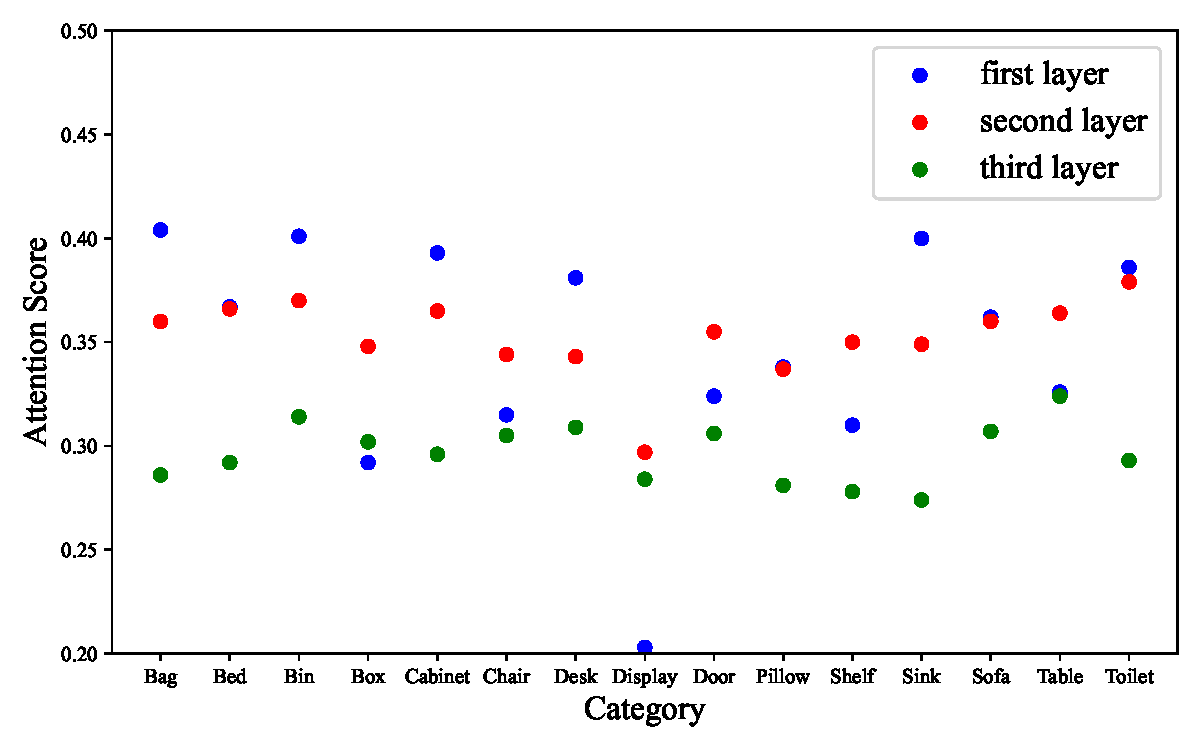
\includegraphics[width=\linewidth]{fig/supplement/hardest.pdf}
    \caption{Local information attention score $z_l$ of LGF. We conduct experiments on ScanObjectNN (PB T50 RS)~\cite{uy2019revisiting} and calculate the average attention score of local information for each category.
}
    \label{fig:attention_score}
    % \vspace{-10pt}
\end{figure}

\begin{figure*}
    \centering
    \begin{subfigure}{0.46\textwidth}
        \centering
        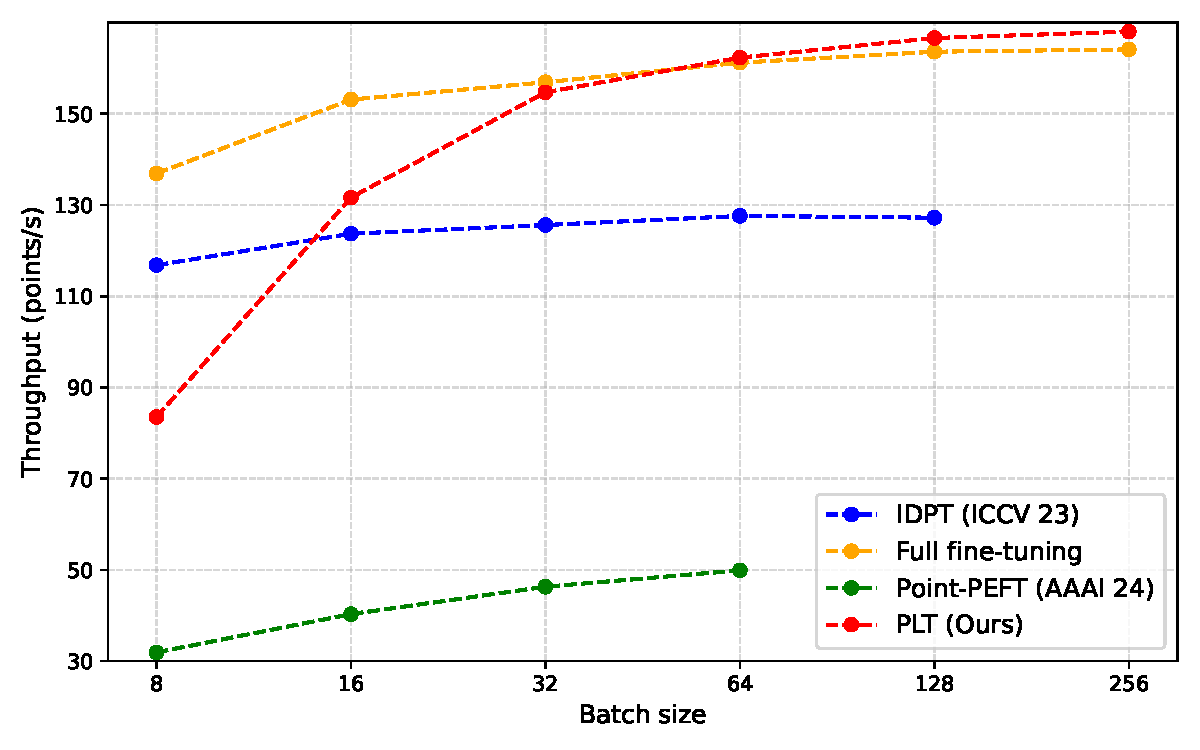
\includegraphics[width=\linewidth]{fig/supplement/performance/train_speed.pdf}
        \caption{Train Speed}
        \label{fig:per1}
    \end{subfigure}
    \hfill
    \begin{subfigure}{0.46\textwidth}
        \centering
        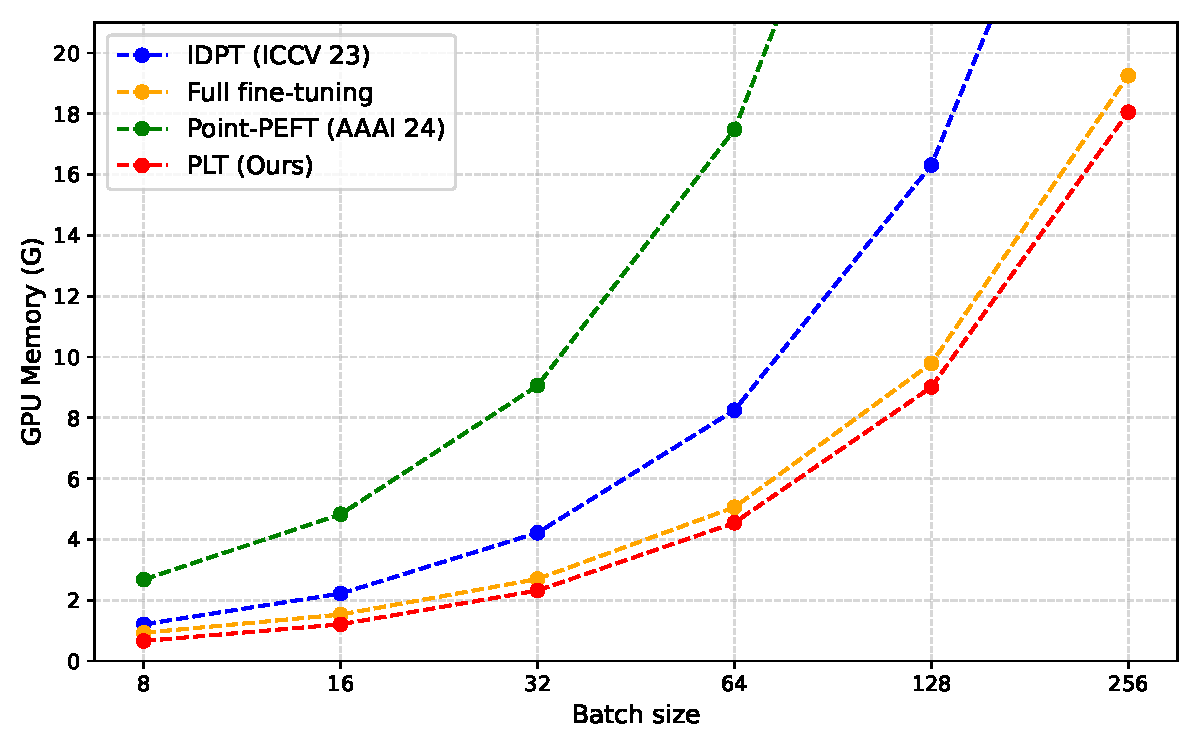
\includegraphics[width=\linewidth]{fig/supplement/performance/train_memory.pdf}
        \caption{Train Memory}
        \label{fig:per2}
    \end{subfigure}
    \hfill
    \begin{subfigure}{0.46\textwidth}
        \centering
        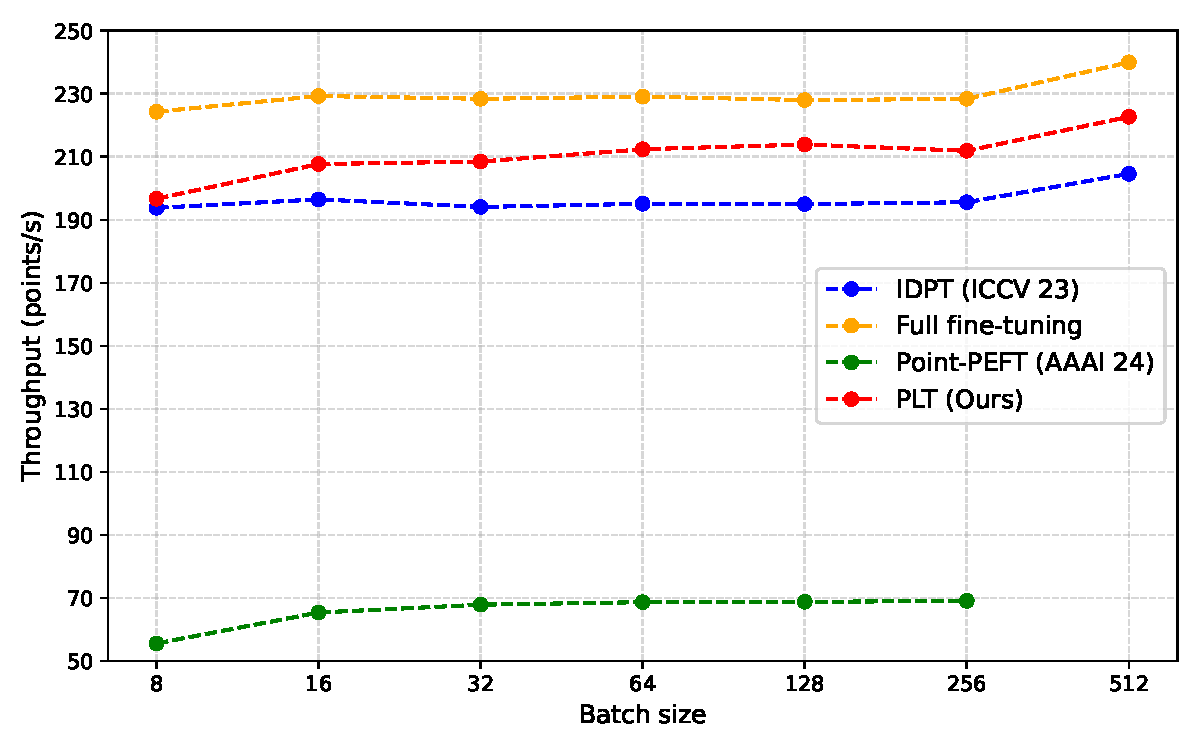
\includegraphics[width=\linewidth]{fig/supplement/performance/infer_speed.pdf}
        \caption{Infer Speed}
        \label{fig:per3}
    \end{subfigure}
    \hfill
    \begin{subfigure}{0.46\textwidth}
        \centering
        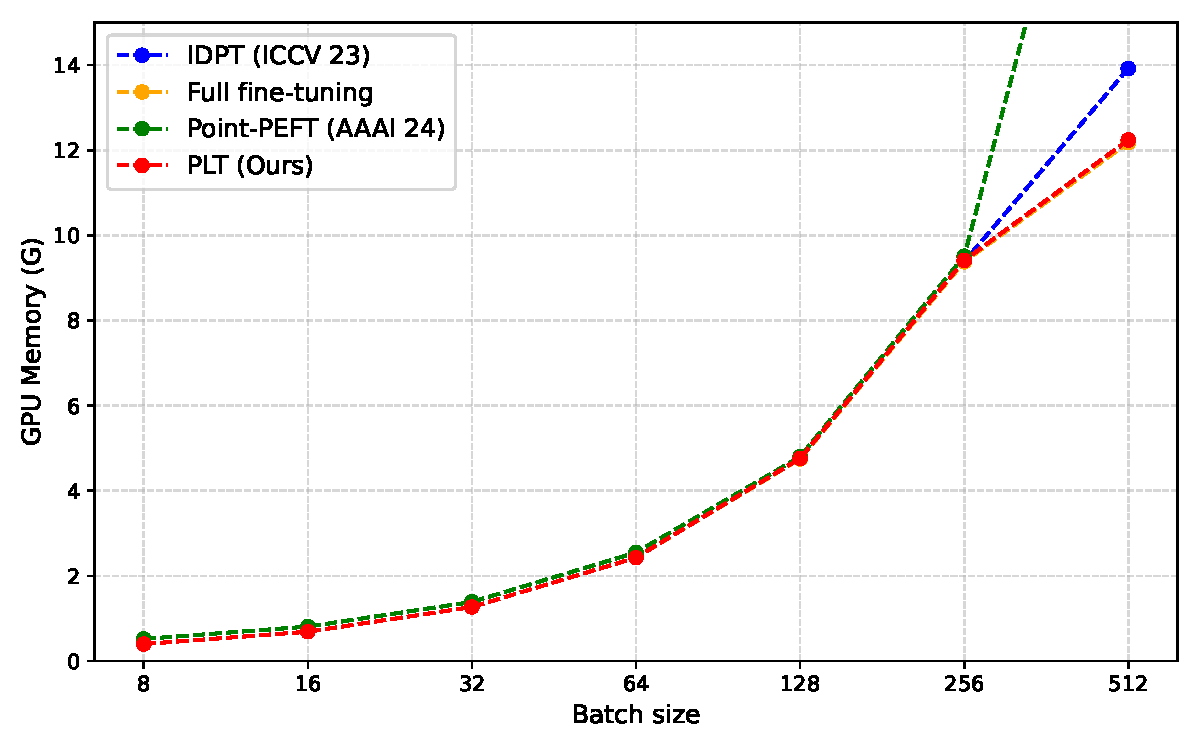
\includegraphics[width=\linewidth]{fig/supplement/performance/infer_memory.pdf}
        \caption{Infer Memory}
        \label{fig:per4}
    \end{subfigure}
    \hfill
    \caption{Comparison of performance between Our PLT and previous methods. We conduct experiments on the hardest variant (i.e., PB\_T50\_RS) of ScanObjectNN~\cite{uy2019revisiting} with Point-MAE baseline~\cite{pang2022masked}. Throughput is measured on a single RTX 3090 GPU.}
    \label{fig:performance}
\end{figure*}

\subsection{Visualization}

\textbf{The Visualization of t-SNE Analysis}. Fig.~\ref{fig:tsne} presents the t-SNE~\cite{van2008visualizing} visualizations of feature manifolds generated by fully fine-tuned methods, point-cloud-specific fine-tuning approaches such as IDPT~\cite{zha2023instance} and DAPT~\cite{zhou2024dynamic}, and our proposed PLT, all trained on the ScanObjectNN PB\_T50\_RS dataset~\cite{uy2019revisiting}. The dispersion of points between categories in the t-SNE plot reflects the quality of the model's feature representation—greater inter-cluster dispersion and smaller intra-cluster average distance indicate stronger discriminative power, facilitating easier classification.

Notably, our PLT demonstrates significantly greater inter-cluster dispersion and a smaller intra-cluster average distance compared to previous methods. This suggests that our approach effectively enhances feature separation between categories while maintaining compactness within each category, indicative of a superior ability to learn and represent discriminative features.

Furthermore, PLT achieves these results while using fewer learnable parameters, showcasing its efficiency in leveraging pre-trained models for adaptation to downstream tasks. This not only reduces computational cost but also highlights PLT's potential for broader applicability in resource-constrained environments. In comparison to fully fine-tuned and point-cloud-specific methods, PLT strikes an optimal balance between parameter efficiency and representation quality, underscoring its value in point cloud learning tasks.

\textbf{Semantic Segmentation Visualizations}. Fig.~\ref{fig:s3dis_1} presents a qualitative comparison of segmentation results between our proposed PLT method and prior fine-tuning approaches in semantic segmentation tasks on Area 5 of the S3DIS dataset~\cite{armeni20163d}. The comparison highlights the advantages of PLT in addressing common challenges in point cloud segmentation. From the first row of the figure, it is evident that while full fine-tuning is resource-intensive, it struggles to accurately segment object boundaries. This often results in poor boundary delineation and misclassification in continuous regions, primarily due to insufficient capture of local point cloud information. 

A more detailed comparison in the office\_9 scene reveals that methods such as full fine-tuning, IDPT~\cite{zha2023instance}, and DAPT~\cite{zhou2024dynamic} incorrectly classify walls as beams and cluttered regions as ceilings. In contrast, our PLT method successfully segments clutter regions while significantly reducing the misclassification of walls. Similarly, in the office\_35 scene, PLT outperforms other methods in segmenting challenging areas such as the cluttered region and the board. Whereas methods like full fine-tuning, IDPT~\cite{zha2023instance}, and PPT~\cite{zhang2024positional} fail to accurately recognize or segment these regions, PLT demonstrates superior performance, maintaining clarity and precision. 

These results emphasize the ability of the PLT method to deliver outstanding segmentation performance while using far fewer fine-tuning parameters. Compared to other approaches, PLT not only provides clearer segmentation boundaries but also significantly reduces misclassifications, further validating its efficiency and effectiveness for point cloud semantic segmentation tasks.

\begin{figure*}[htbp]
    \centering

    % 第一行左侧的竖排标签
    \begin{minipage}{0.09\textwidth}
        \centering
        Full
        Fine-tuning
    \end{minipage}
    \hfill
    % 第一行图片
    \begin{minipage}{0.22\textwidth}
        \centering
        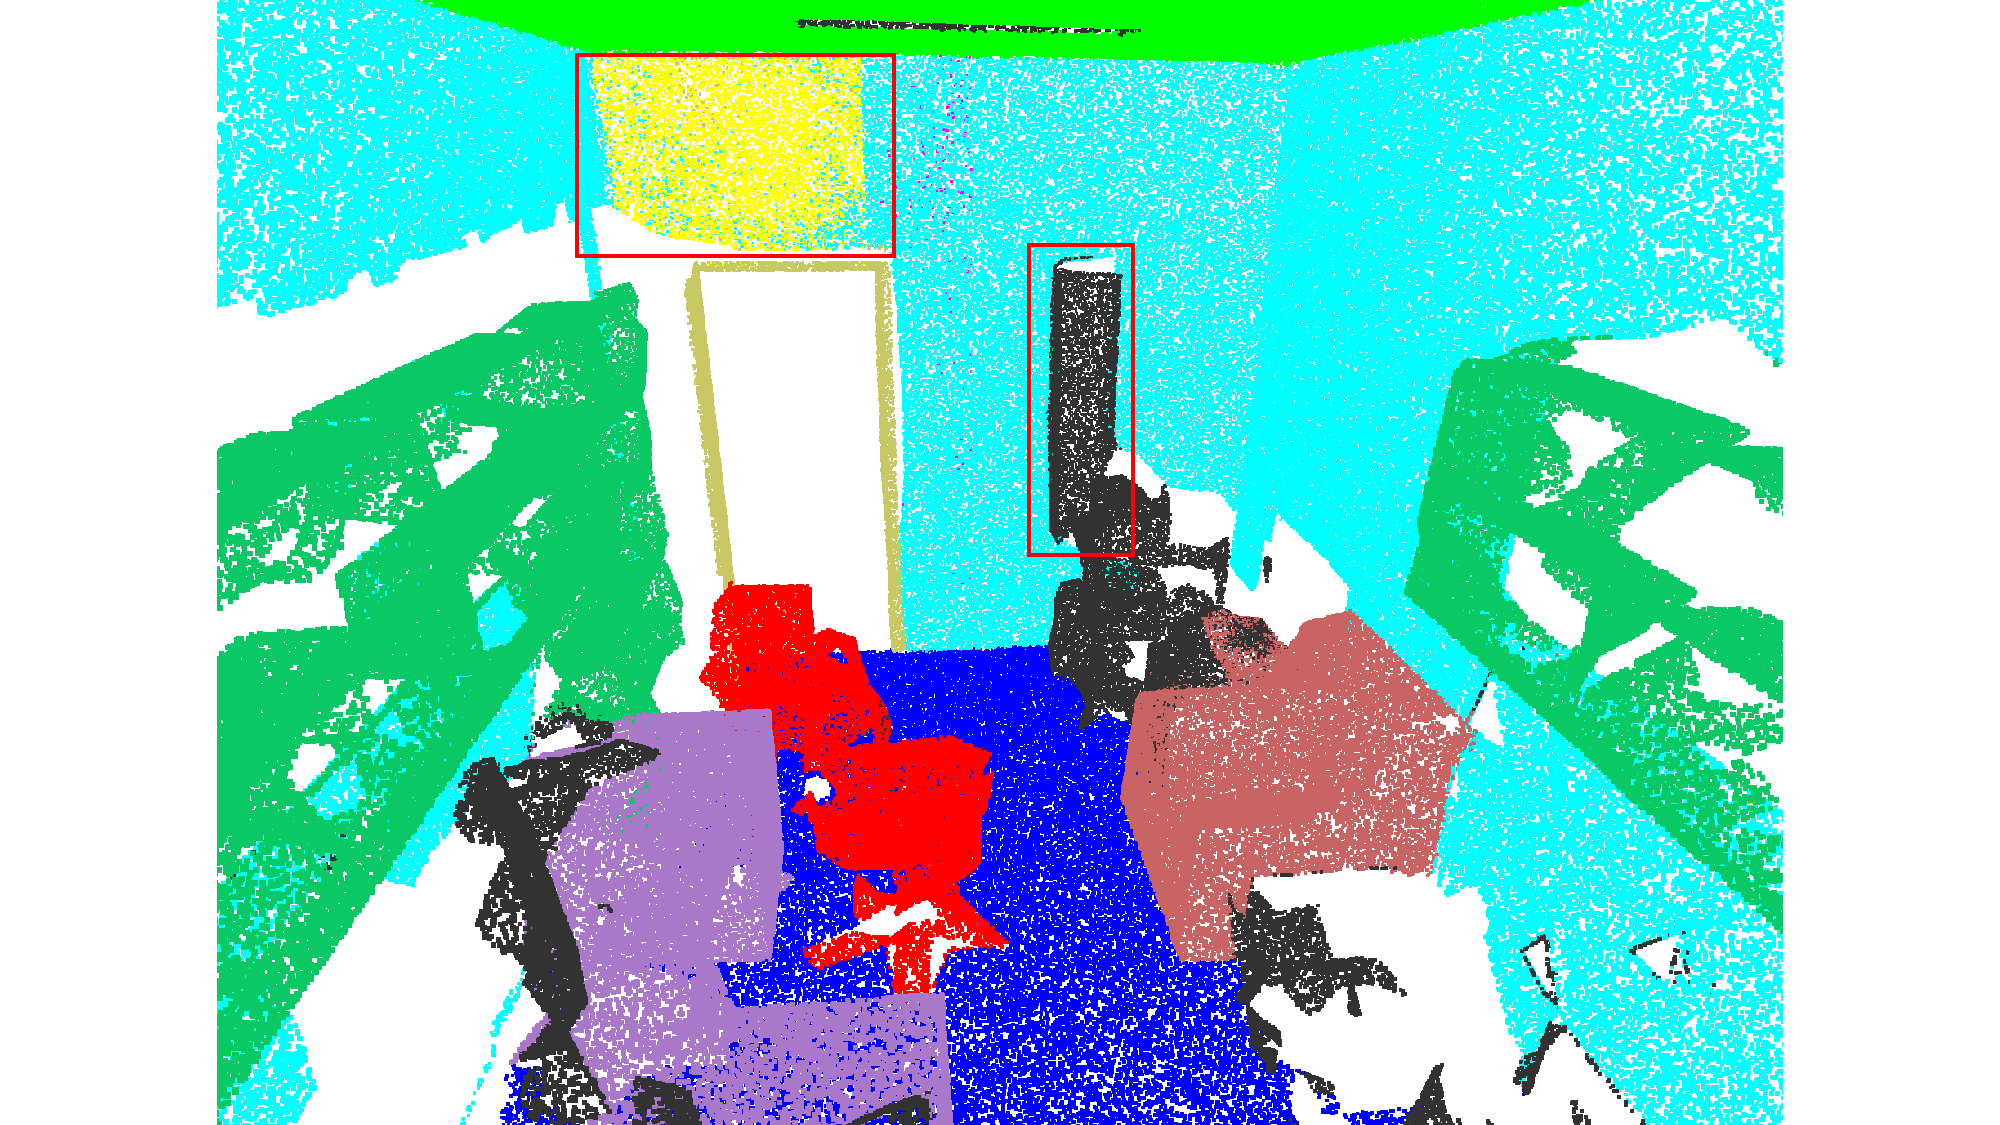
\includegraphics[width=\textwidth]{fig/supplement/semantic_segmentation/office_9/PT_office_9.pdf}
    \end{minipage}
    \hfill
    \begin{minipage}{0.22\textwidth}
        \centering
        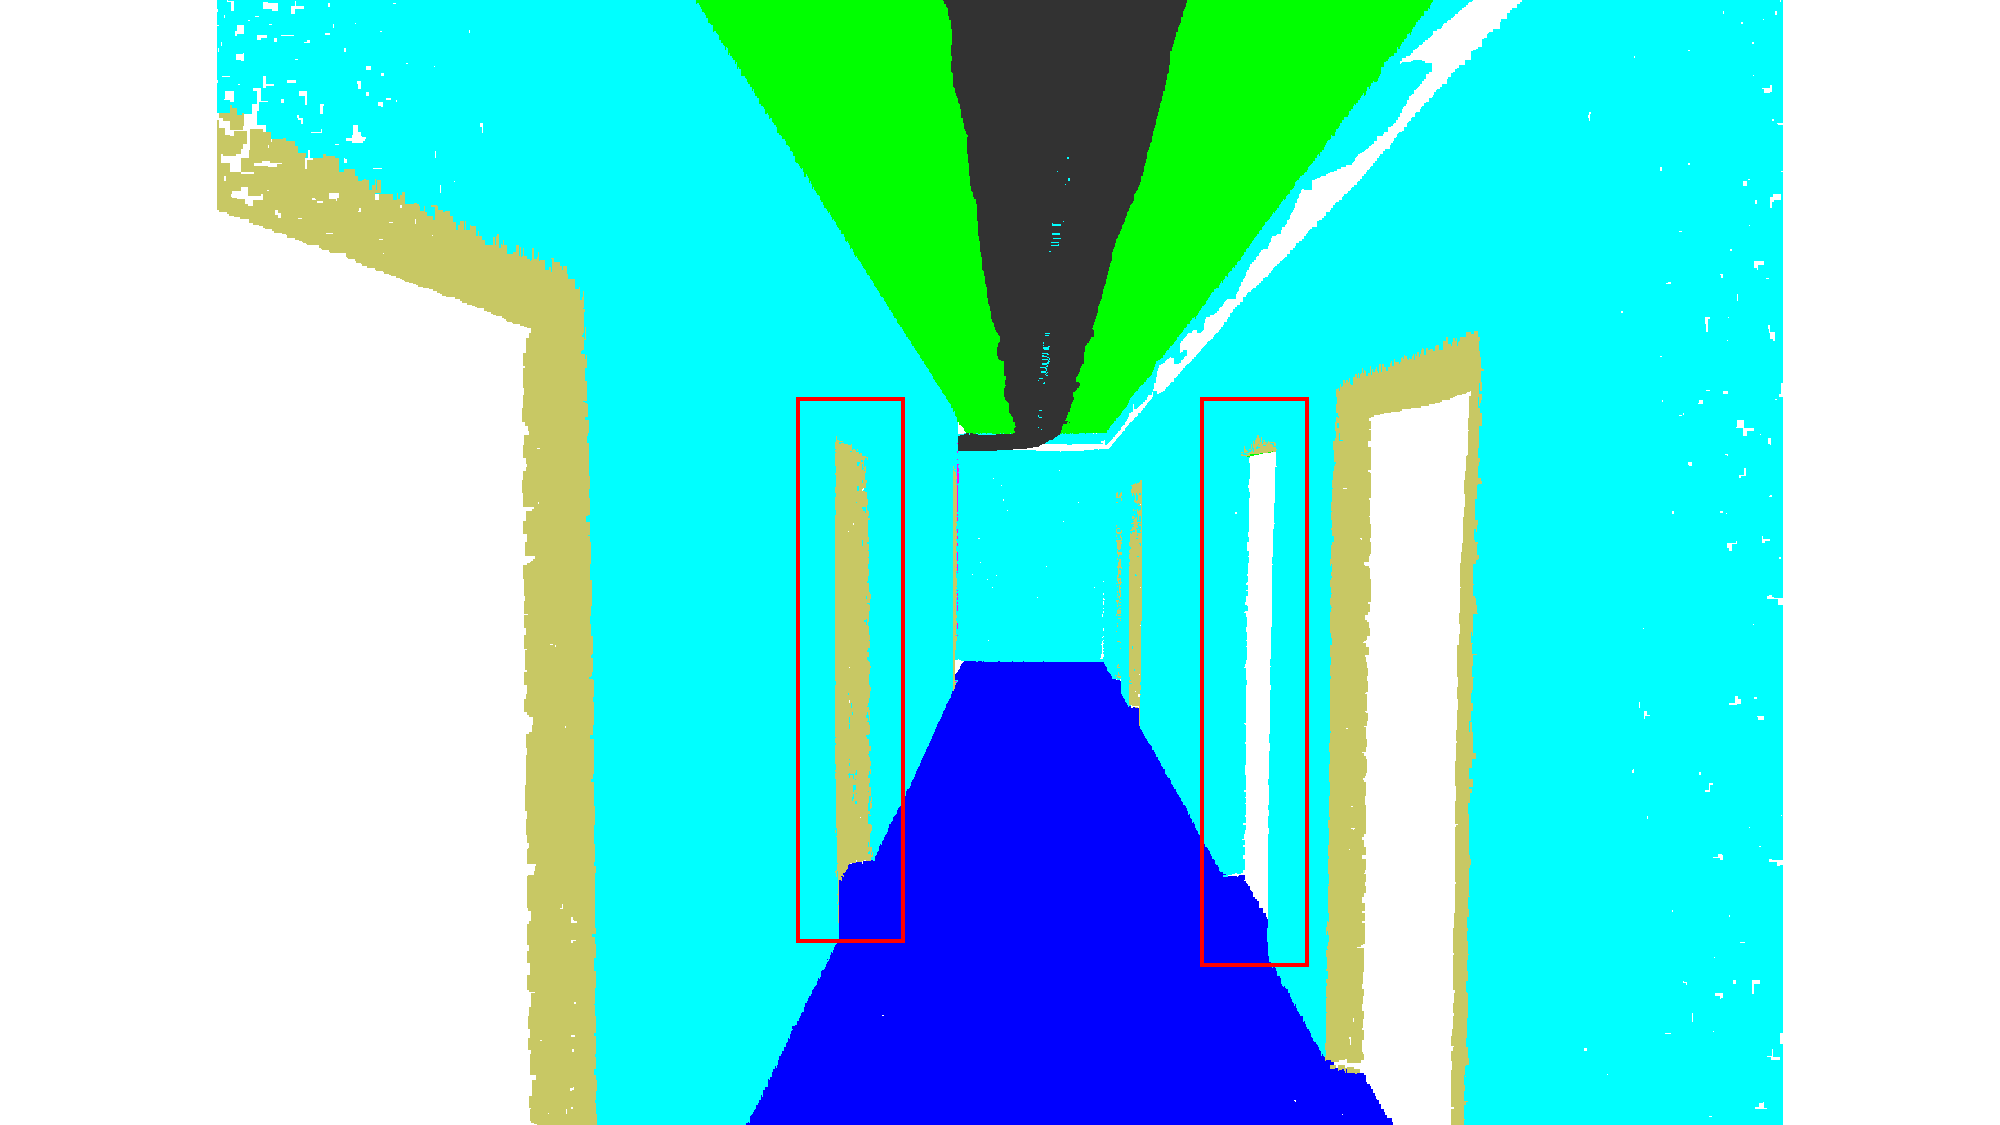
\includegraphics[width=\textwidth]{fig/supplement/semantic_segmentation/hallway_10/PT_hallway_10.pdf} % 替换为你的图片路径
    \end{minipage}
    \hfill
    \begin{minipage}{0.22\textwidth}
        \centering
        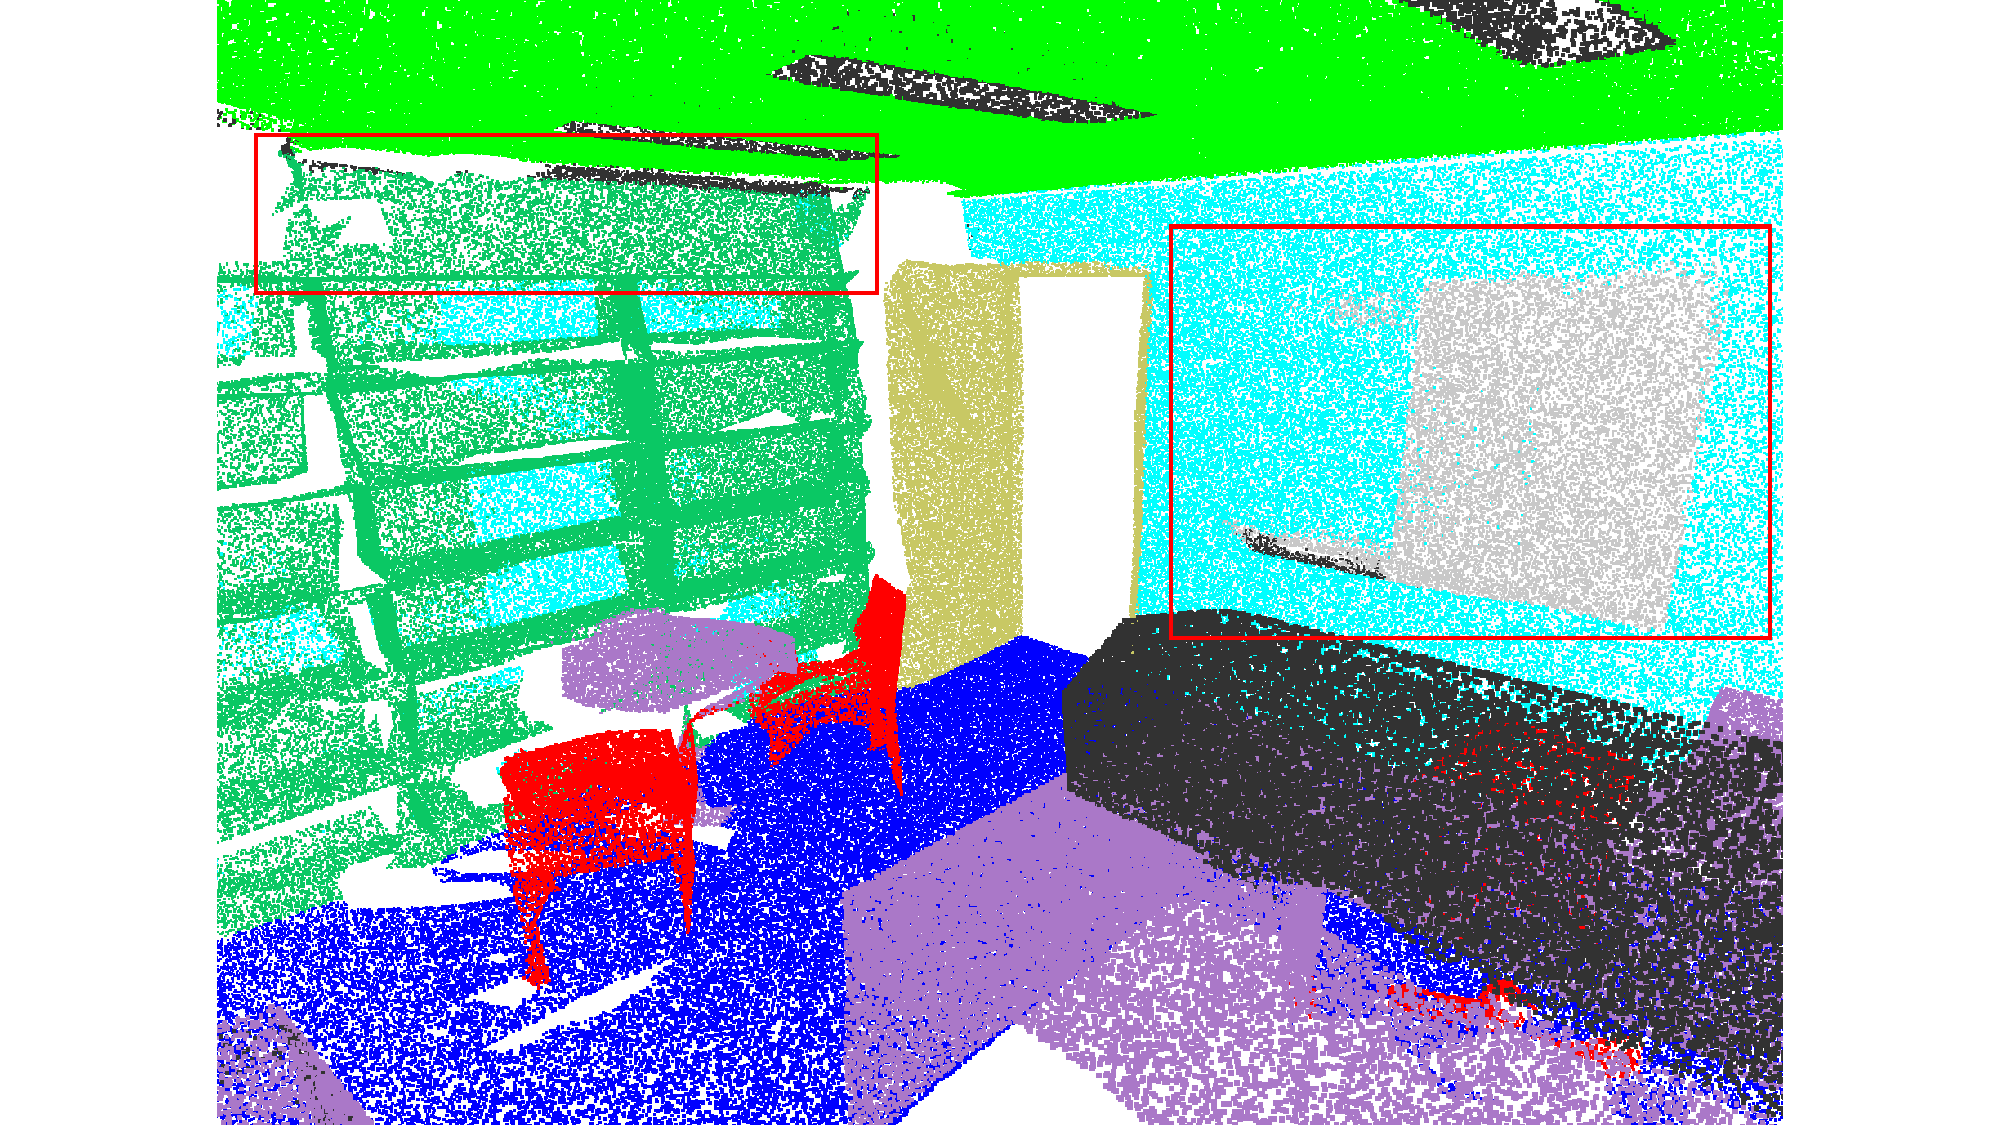
\includegraphics[width=\textwidth]{fig/supplement/semantic_segmentation/office_35/PT_office_35.pdf}
    \end{minipage}
    \hfill
    \begin{minipage}{0.22\textwidth}
        \centering
        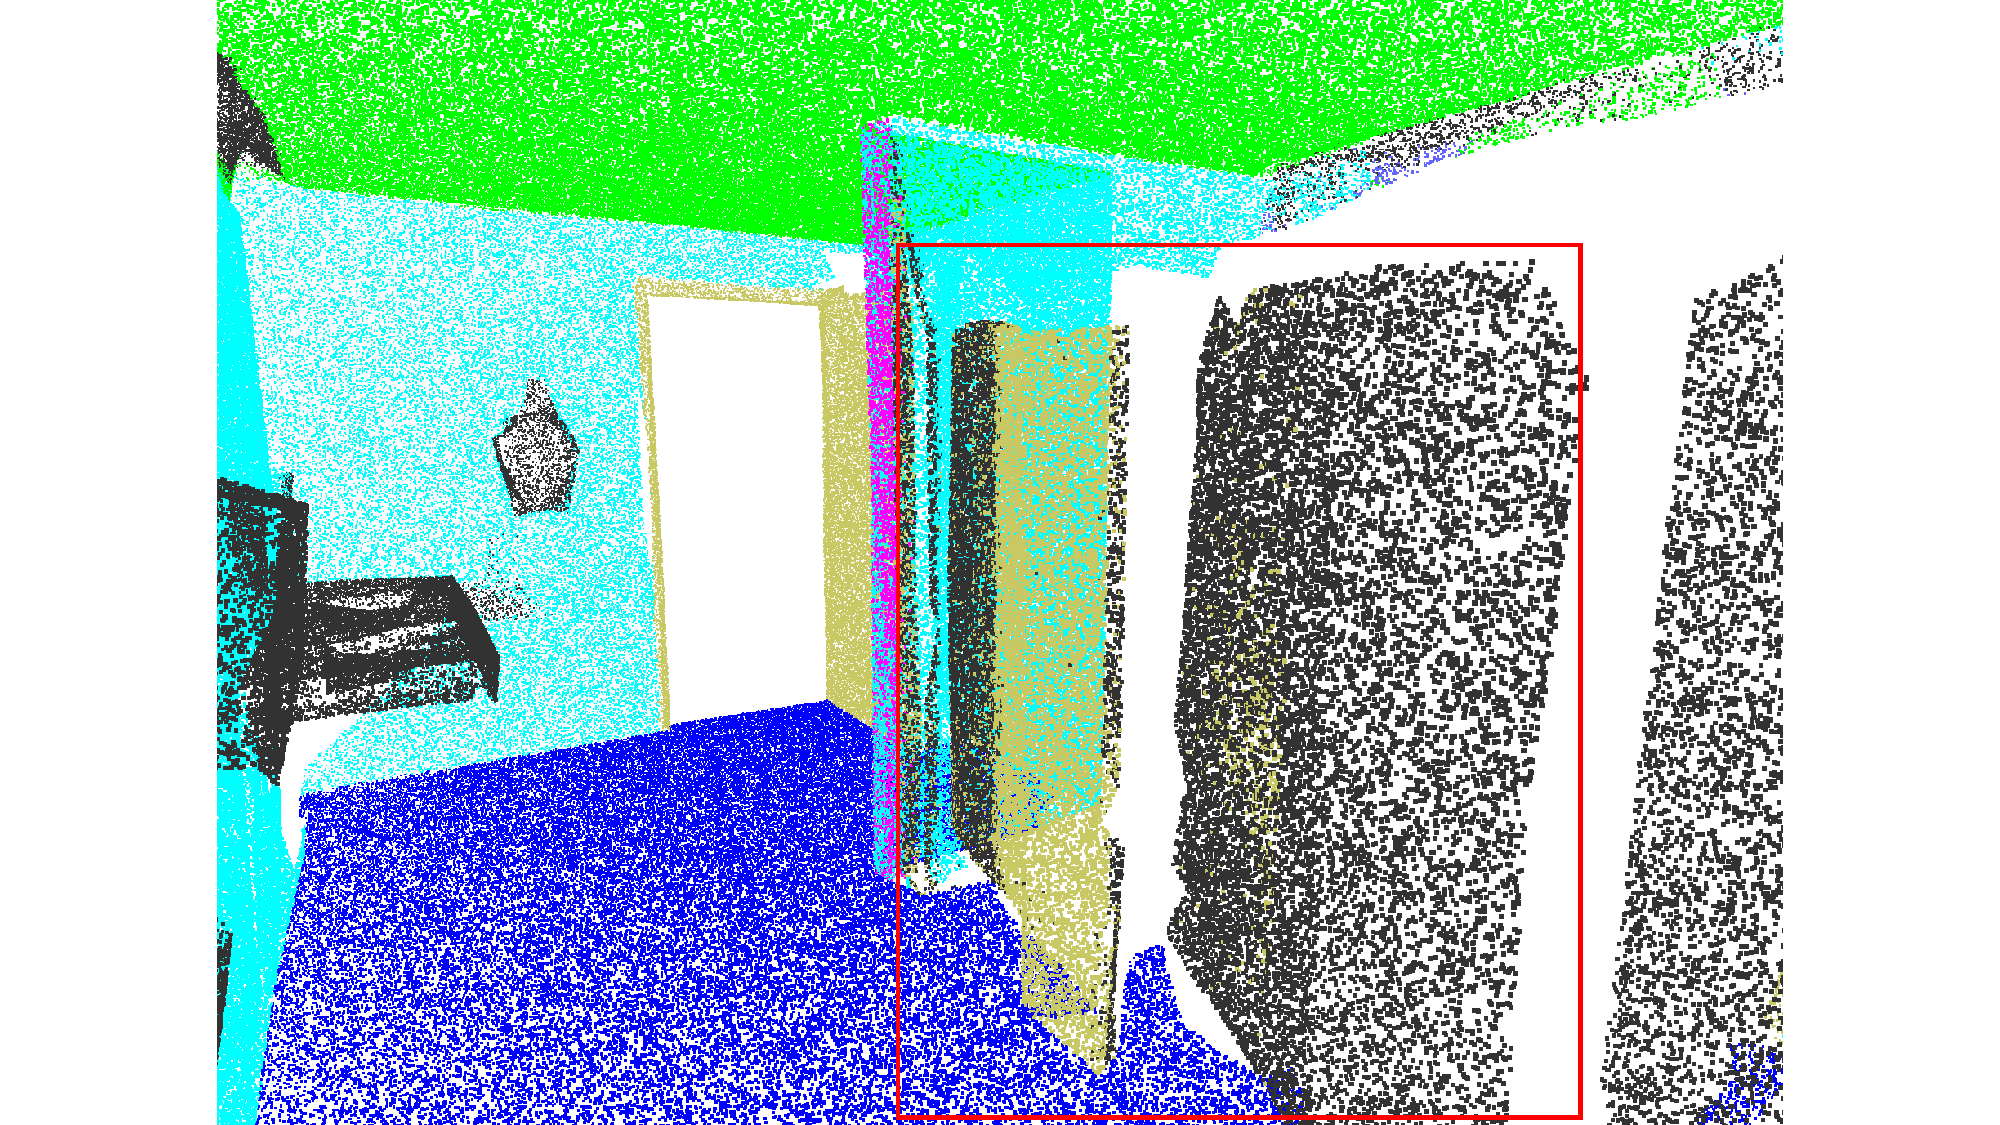
\includegraphics[width=\textwidth]{fig/supplement/semantic_segmentation/wc_2/PT_wc_2.pdf}
    \end{minipage}
    \hfill

    % 换行
    \vspace{0.5em}

    % 第二行左侧的竖排标签
    \begin{minipage}{0.09\textwidth}
        \centering
        DAPT
    \end{minipage}
    \hfill
    % 第二行图片
    \begin{minipage}{0.22\textwidth}
        \centering
        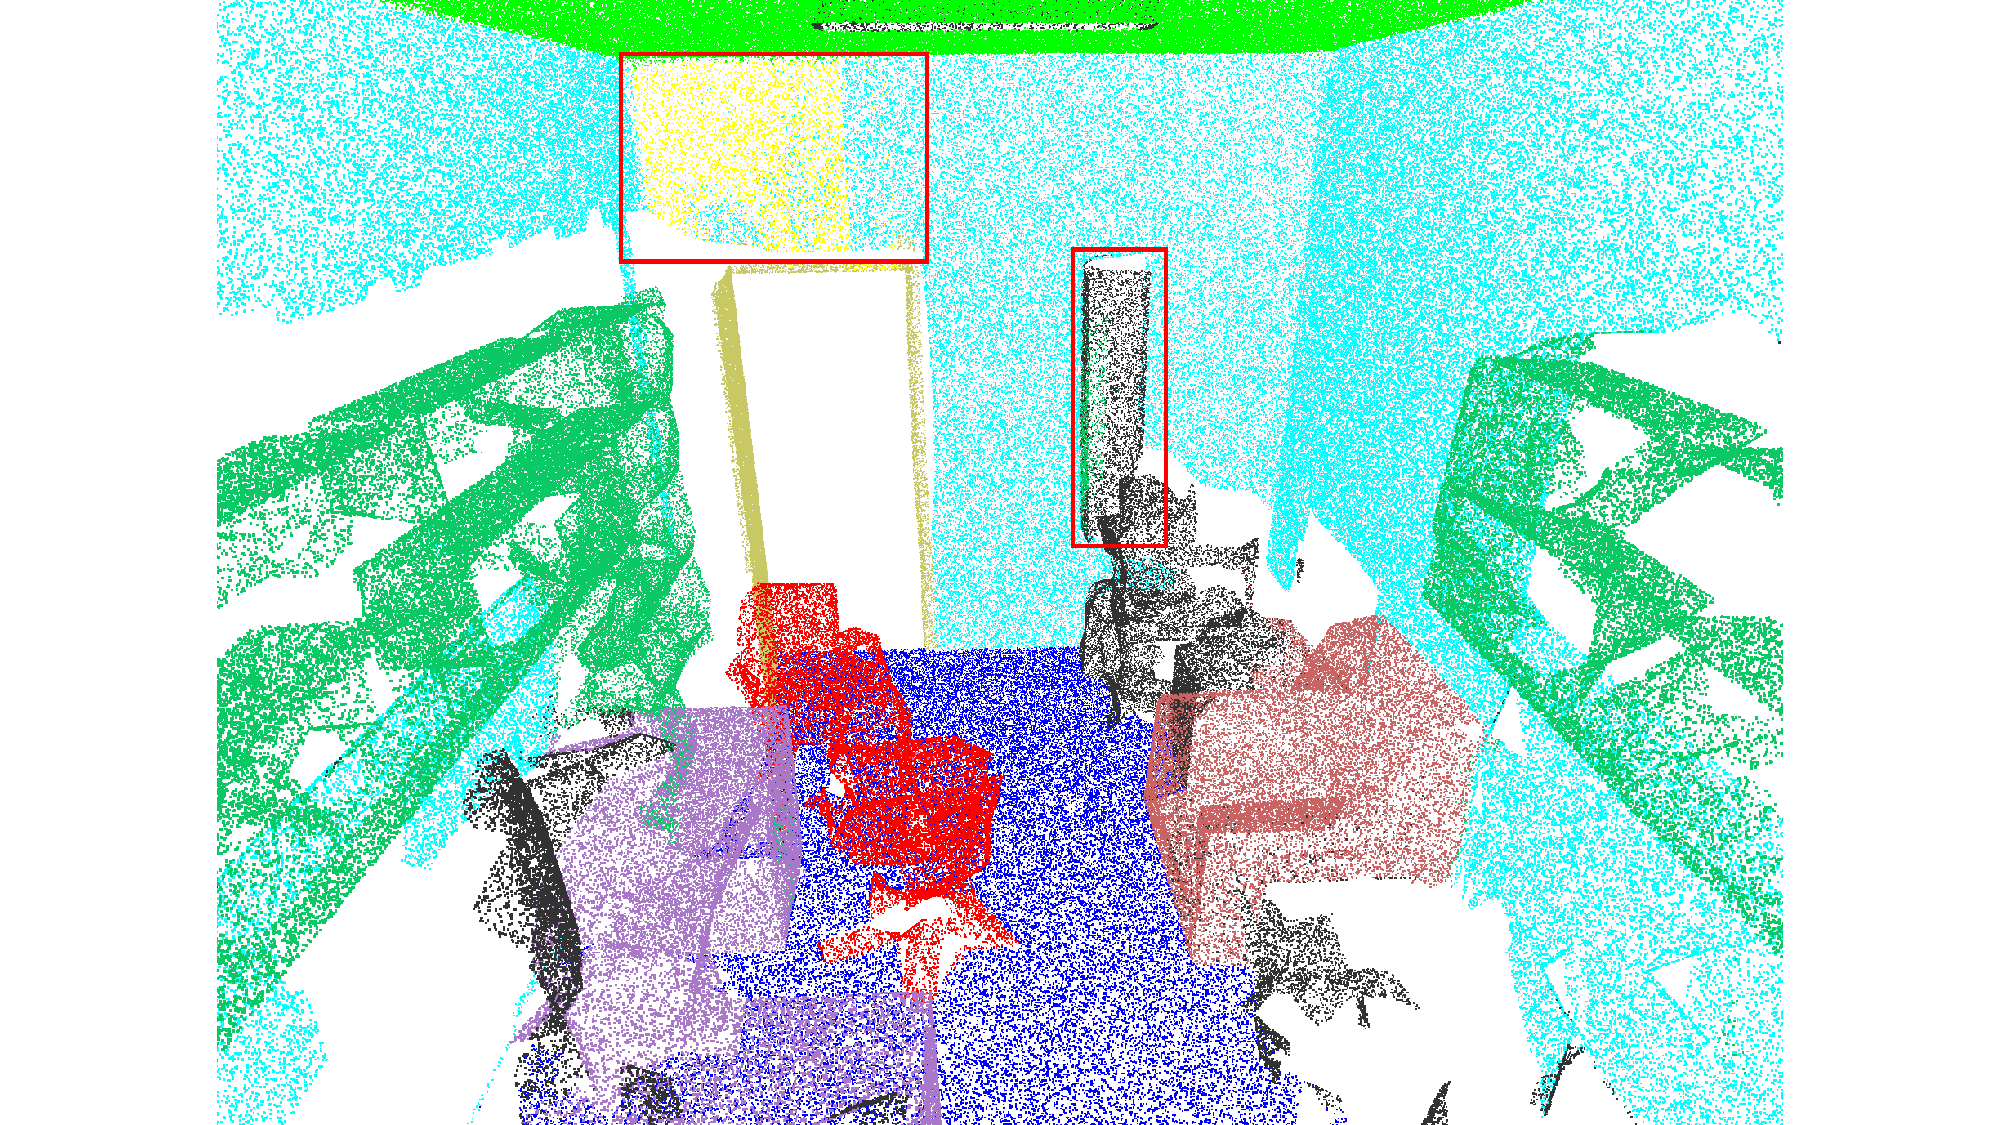
\includegraphics[width=\textwidth]{fig/supplement/semantic_segmentation/office_9/DAPT_office_9.pdf}
    \end{minipage}
    \hfill
    \begin{minipage}{0.22\textwidth}
        \centering
        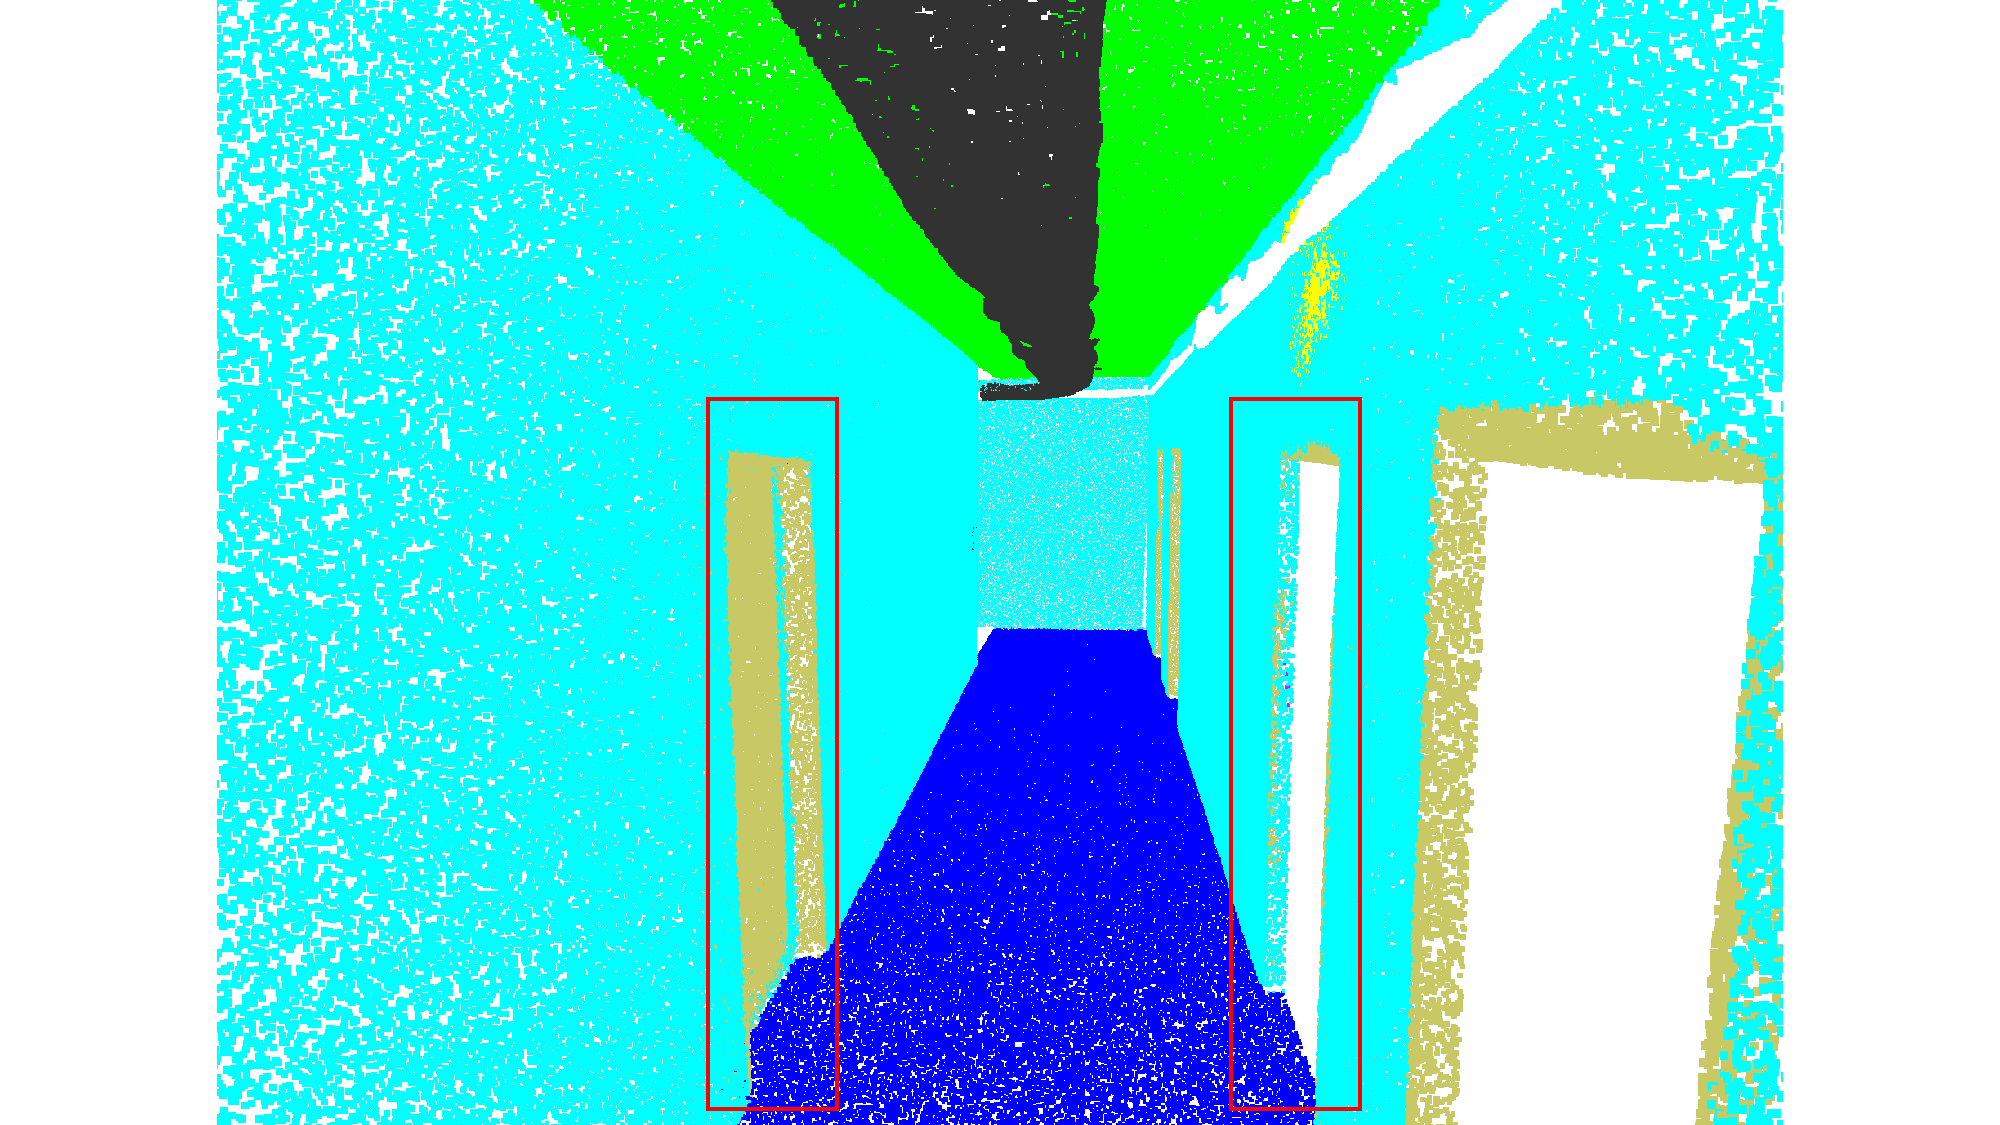
\includegraphics[width=\textwidth]{fig/supplement/semantic_segmentation/hallway_10/DAPT_hallway_10.pdf}
    \end{minipage}
    \hfill
    \begin{minipage}{0.22\textwidth}
        \centering
        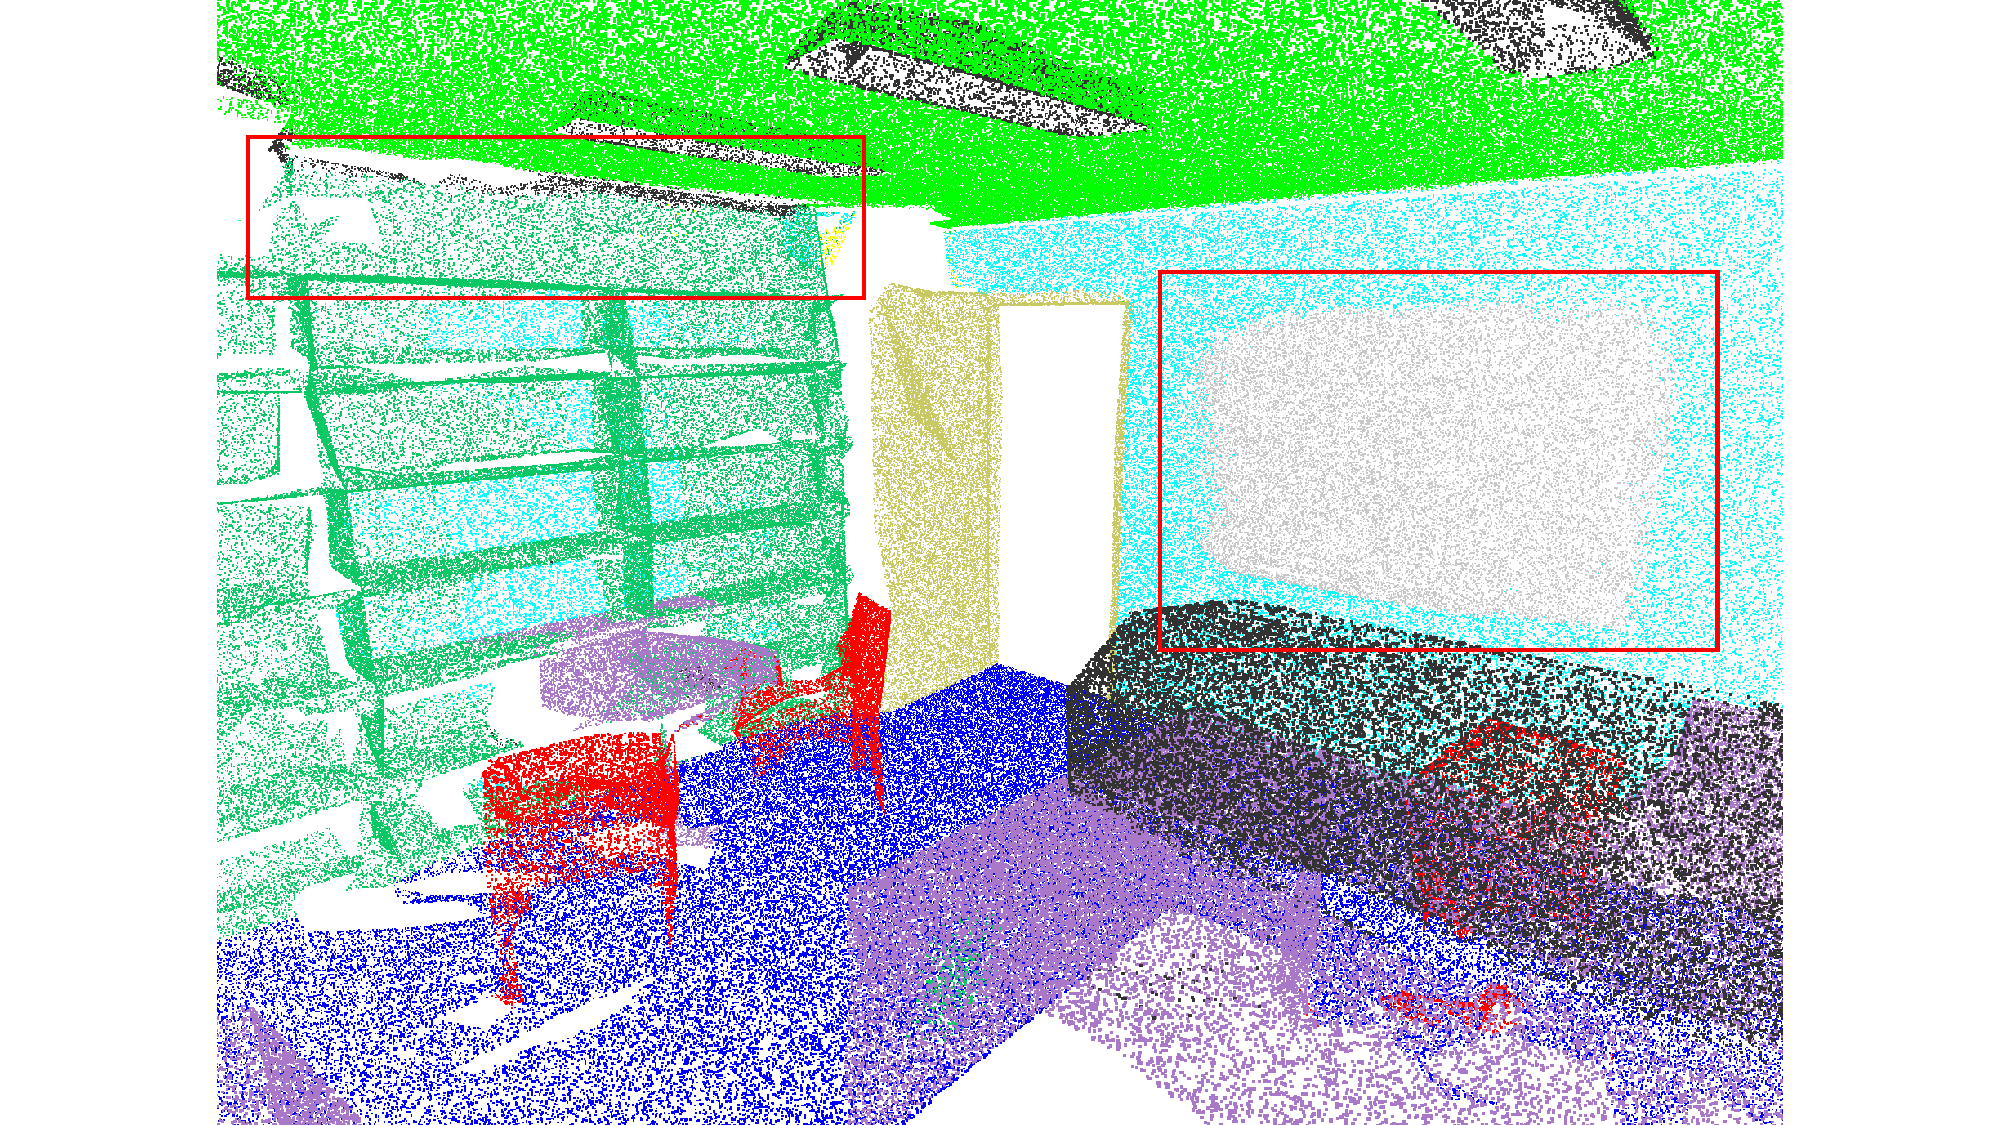
\includegraphics[width=\textwidth]{fig/supplement/semantic_segmentation/office_35/DAPT_office_35.pdf}
    \end{minipage}
    \hfill
    \begin{minipage}{0.22\textwidth}
        \centering
        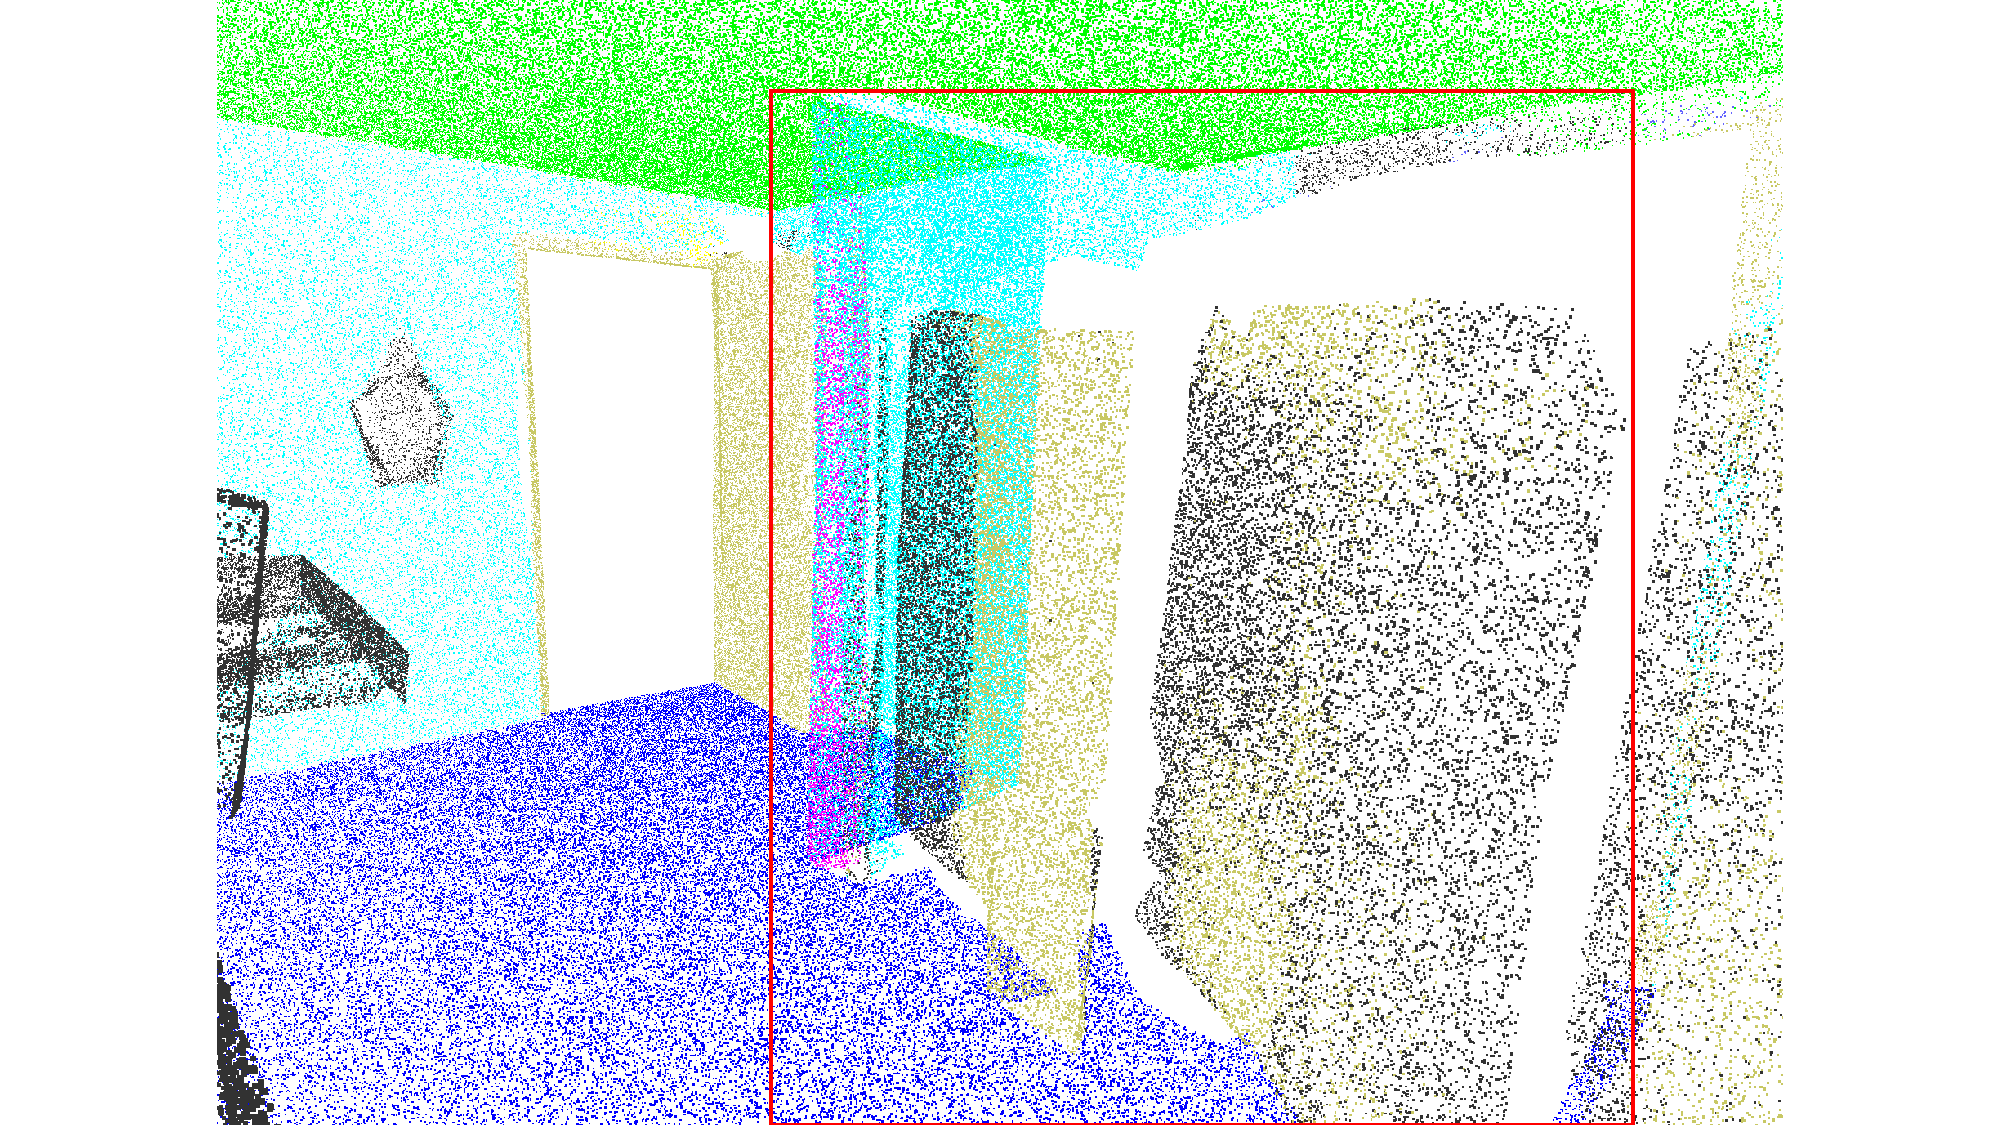
\includegraphics[width=\textwidth]{fig/supplement/semantic_segmentation/wc_2/DAPT_wc_2.pdf}
    \end{minipage}
    \hfill

    % 换行
    \vspace{0.5em}

    % 第三行左侧的竖排标签
    \begin{minipage}{0.09\textwidth}
        \centering
        IDPT
    \end{minipage}
    \hfill
    % 第三行图片
    \begin{minipage}{0.22\textwidth}
        \centering
        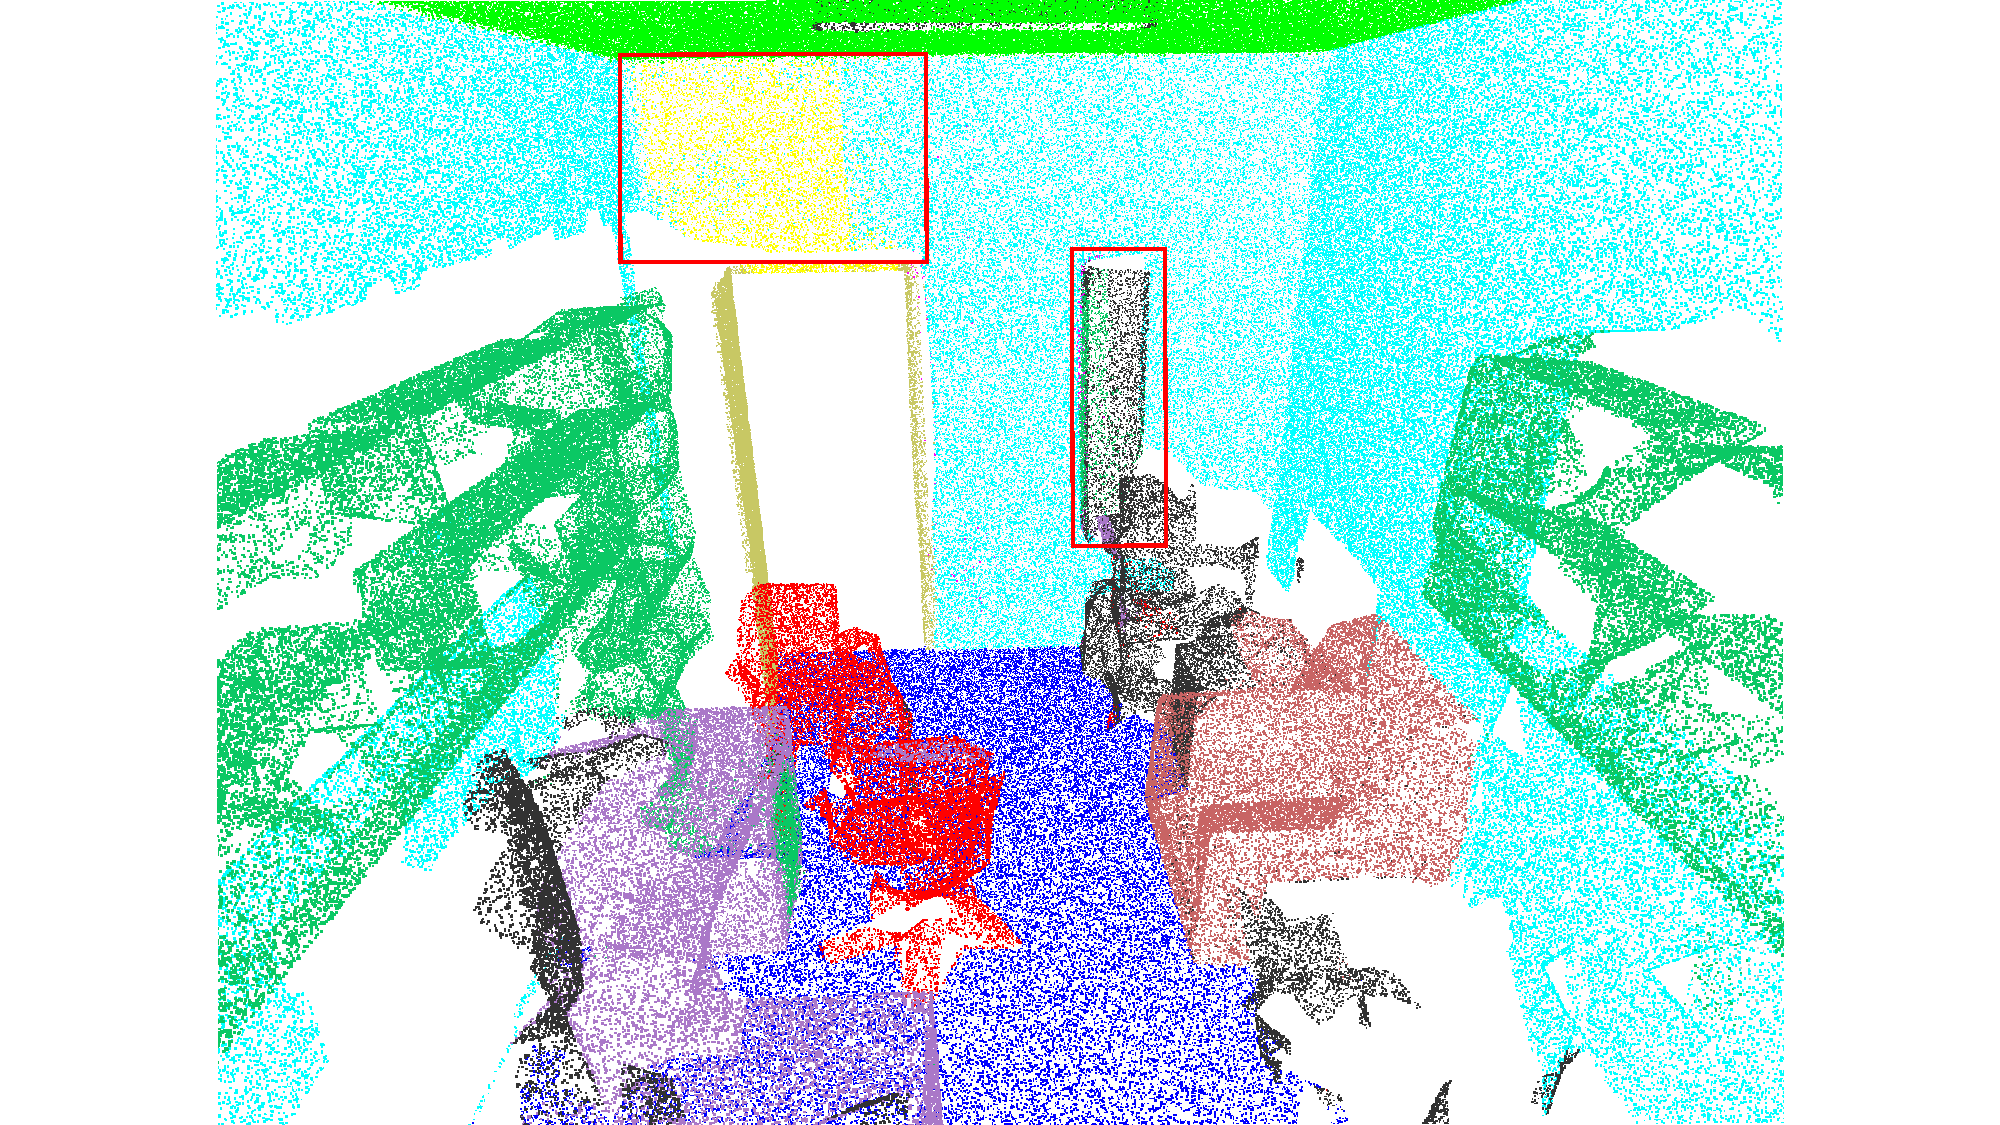
\includegraphics[width=\textwidth]{fig/supplement/semantic_segmentation/office_9/IDPT_office_9.pdf}
    \end{minipage}
    \hfill
    \begin{minipage}{0.22\textwidth}
        \centering
        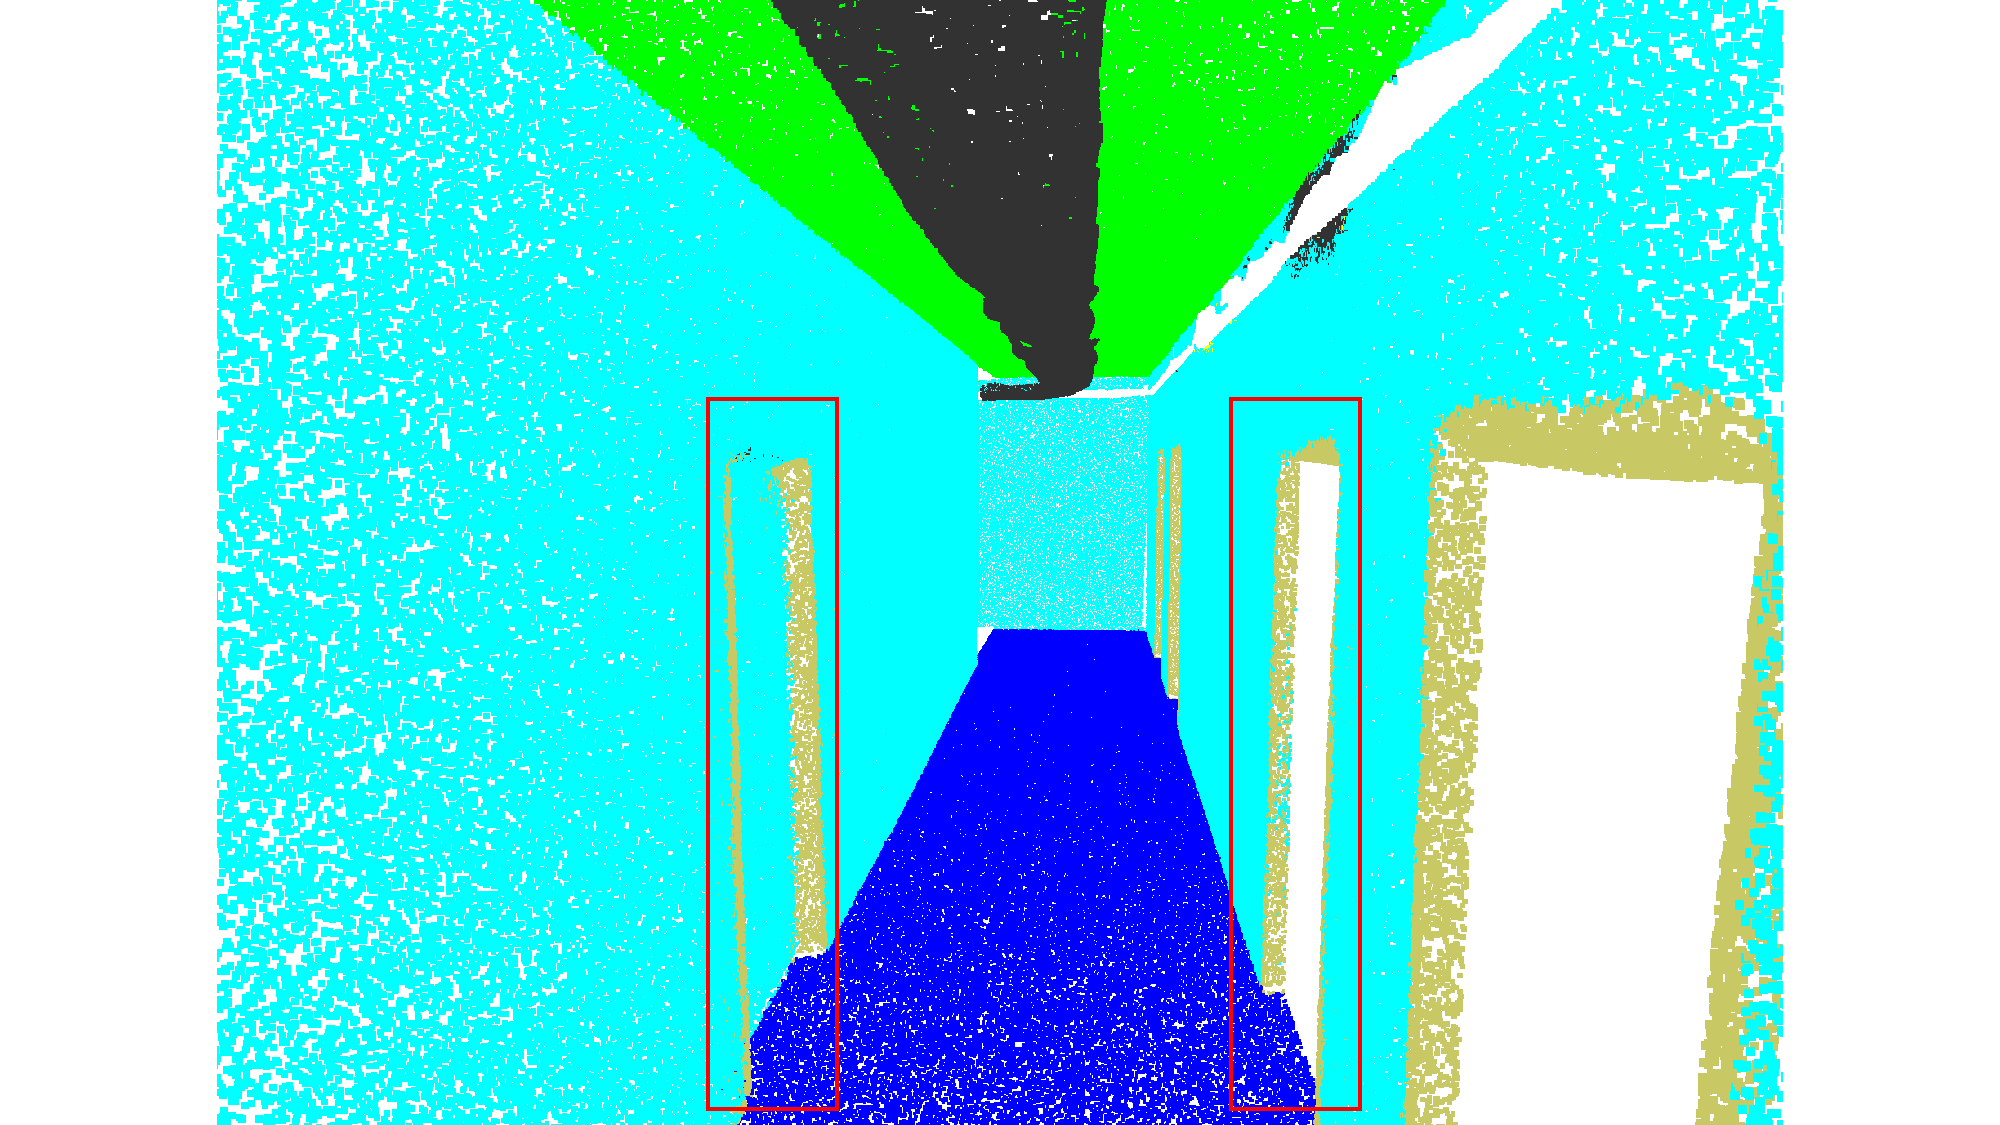
\includegraphics[width=\textwidth]{fig/supplement/semantic_segmentation/hallway_10/IDPT_hallway_10.pdf}
    \end{minipage}
    \hfill
    \begin{minipage}{0.22\textwidth}
        \centering
        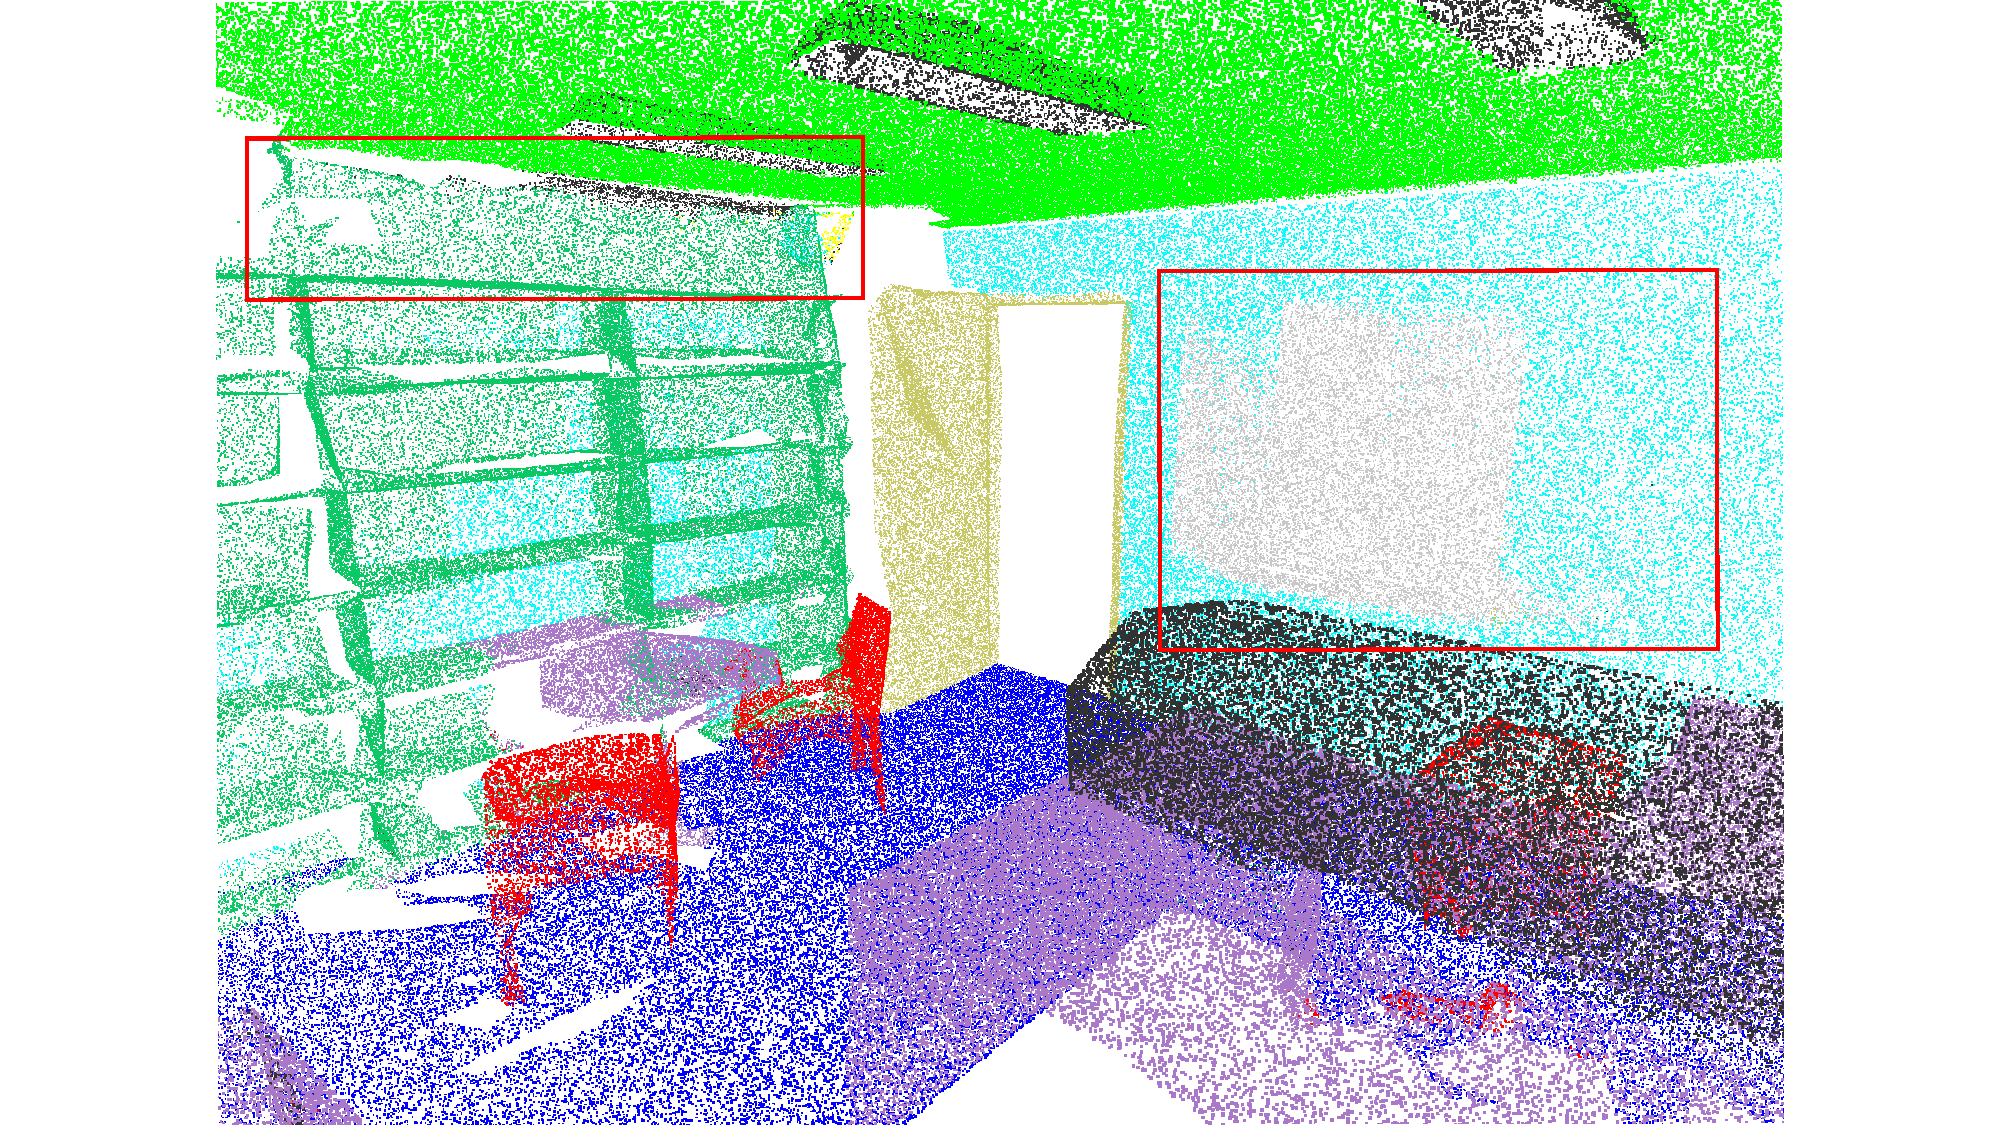
\includegraphics[width=\textwidth]{fig/supplement/semantic_segmentation/office_35/IDPT_office_35.pdf}
    \end{minipage}
    \hfill
    \begin{minipage}{0.22\textwidth}
        \centering
        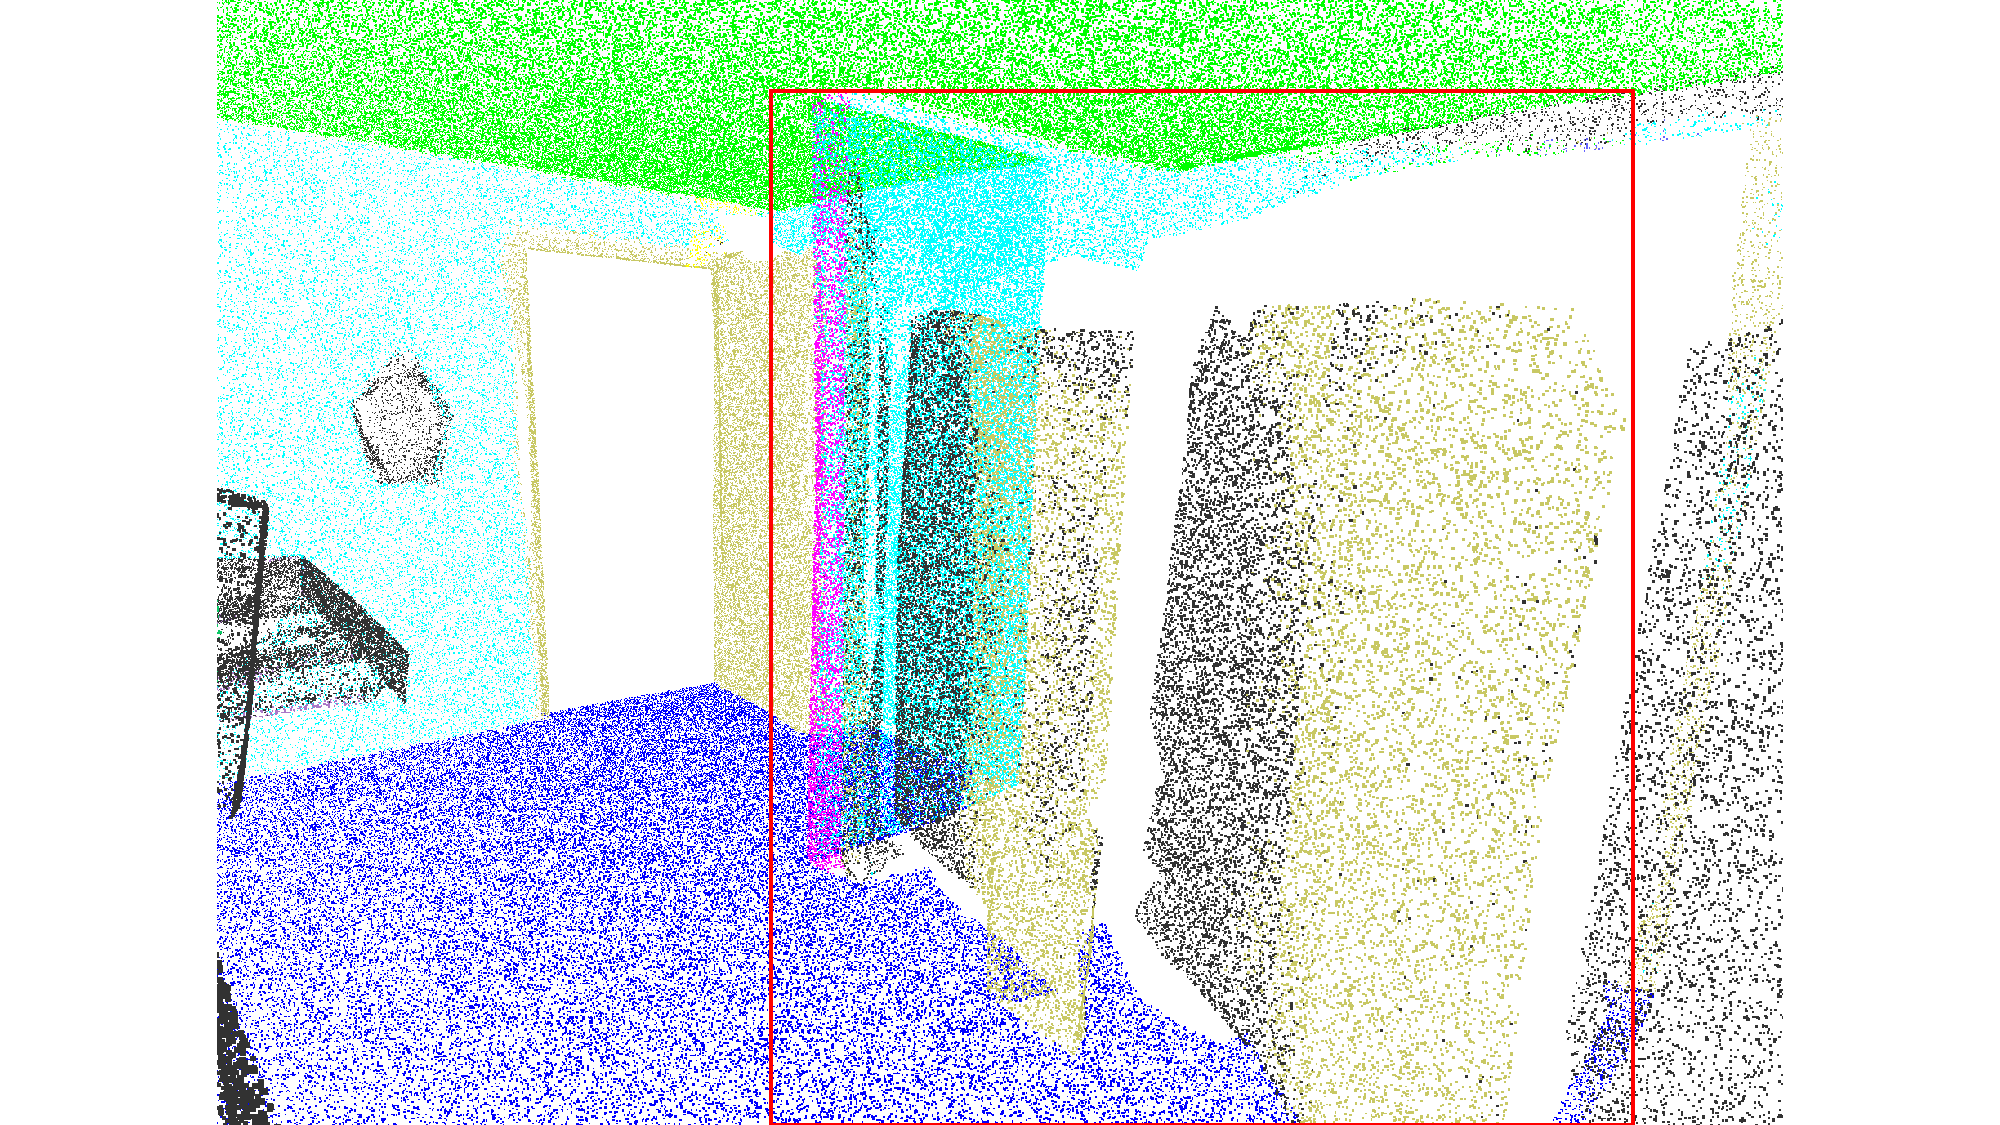
\includegraphics[width=\textwidth]{fig/supplement/semantic_segmentation/wc_2/IDPT_wc_2.pdf}
    \end{minipage}
    \hfill

    % 换行
    \vspace{0.5em}

    % 第四行左侧的竖排标签
    \begin{minipage}{0.09\textwidth}
        \centering
        PPT
    \end{minipage}
    \hfill
    % 第四行图片
    \begin{minipage}{0.22\textwidth}
        \centering
        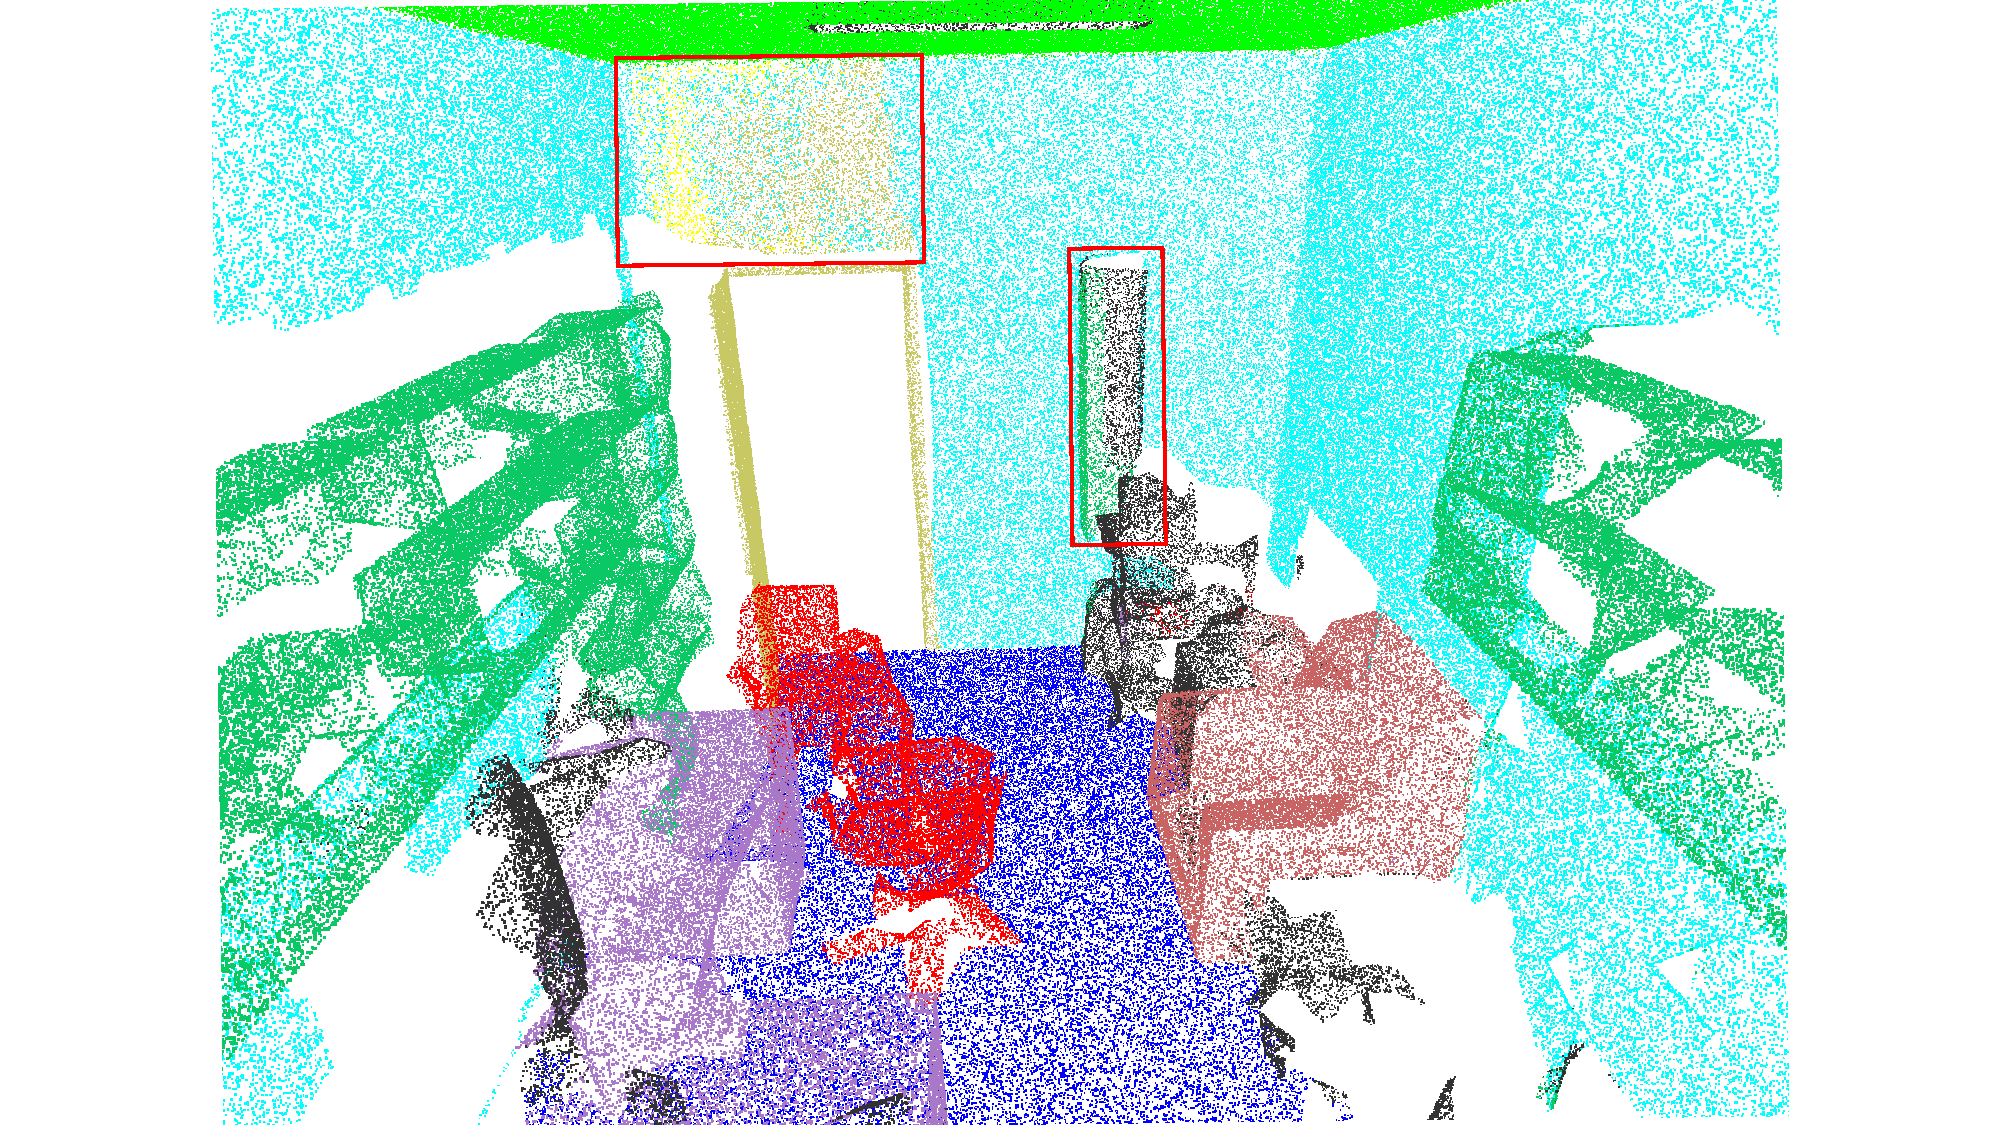
\includegraphics[width=\textwidth]{fig/supplement/semantic_segmentation/office_9/PPT_office_9.pdf}
    \end{minipage}
    \hfill
     \begin{minipage}{0.22\textwidth}
        \centering
        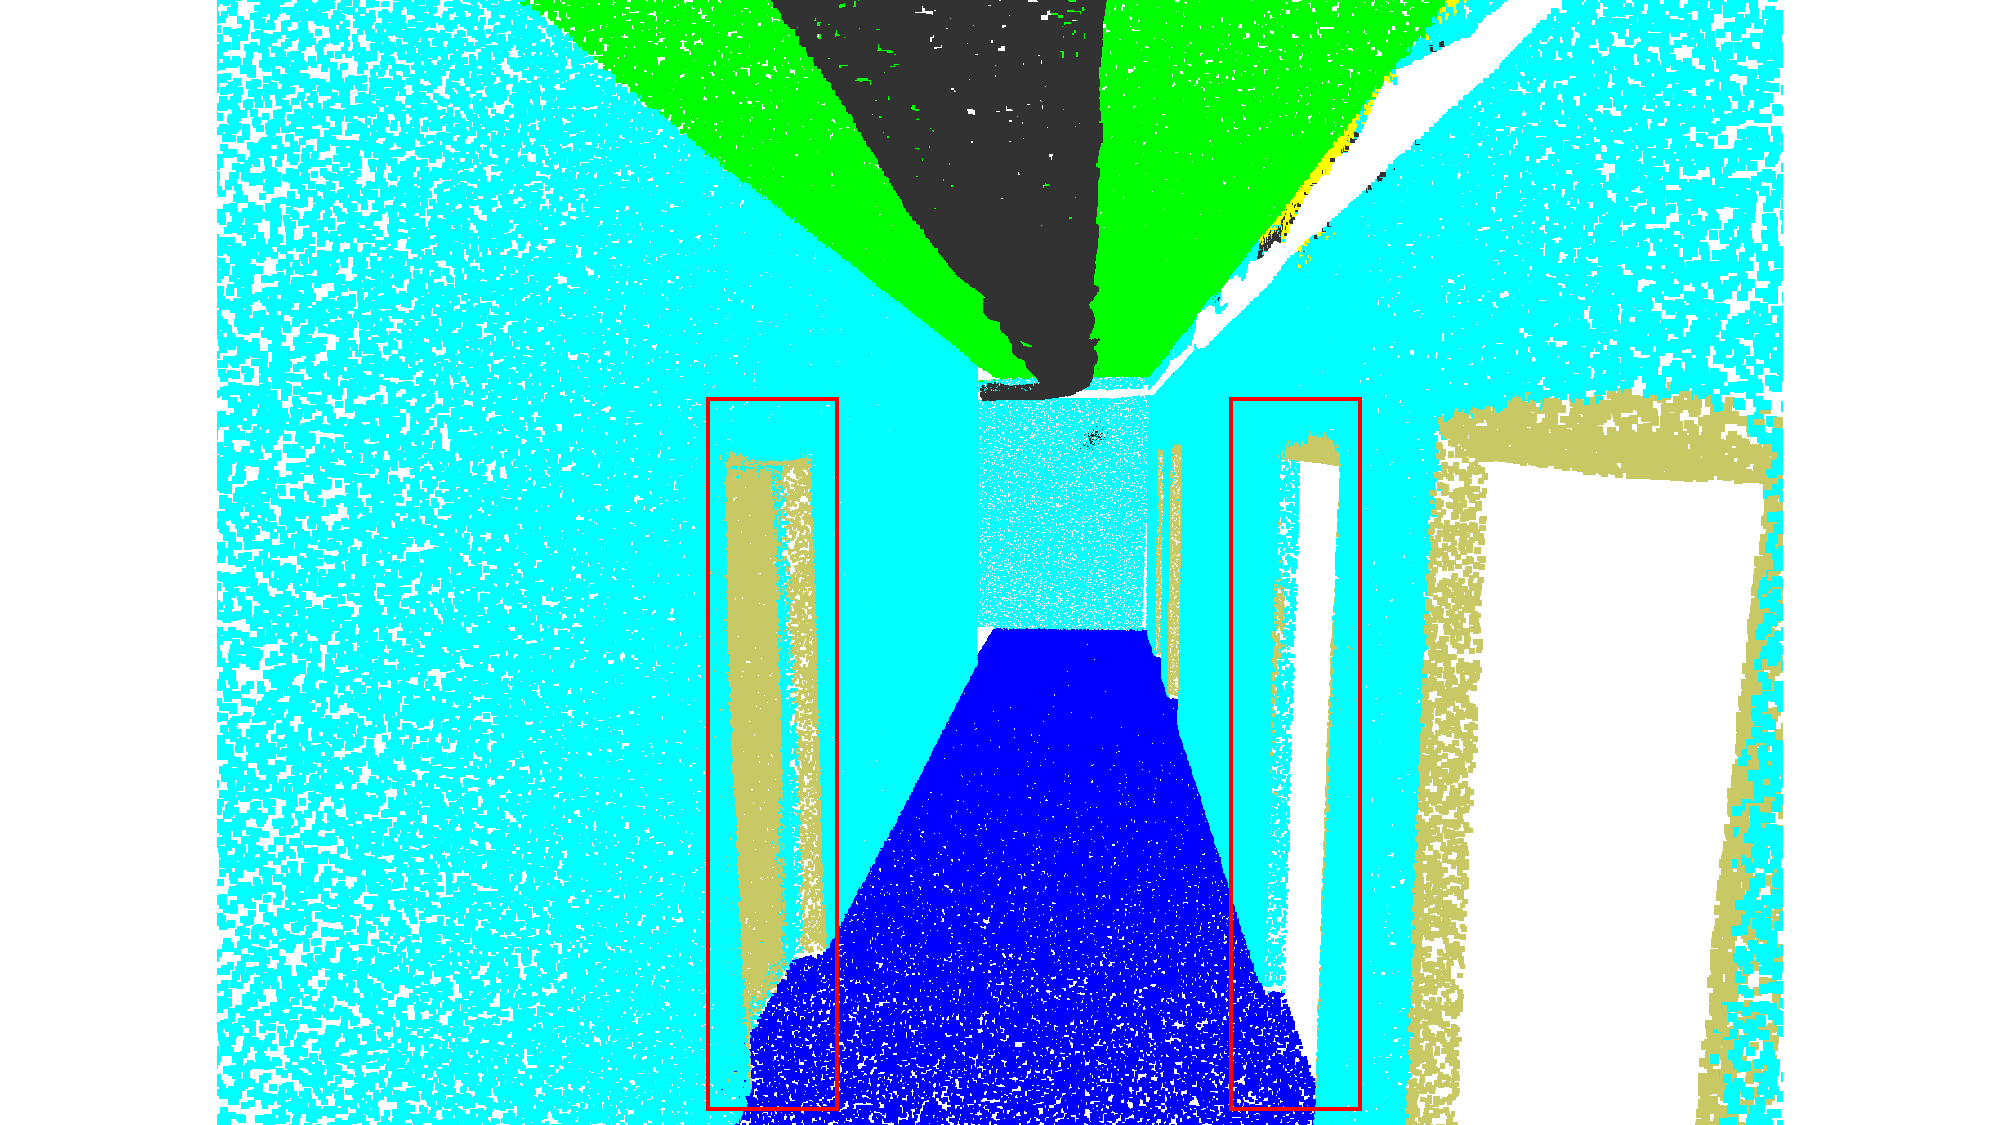
\includegraphics[width=\textwidth]{fig/supplement/semantic_segmentation/hallway_10/PPT_hallway_10.pdf}
    \end{minipage}
    \hfill
    \begin{minipage}{0.22\textwidth}
        \centering
        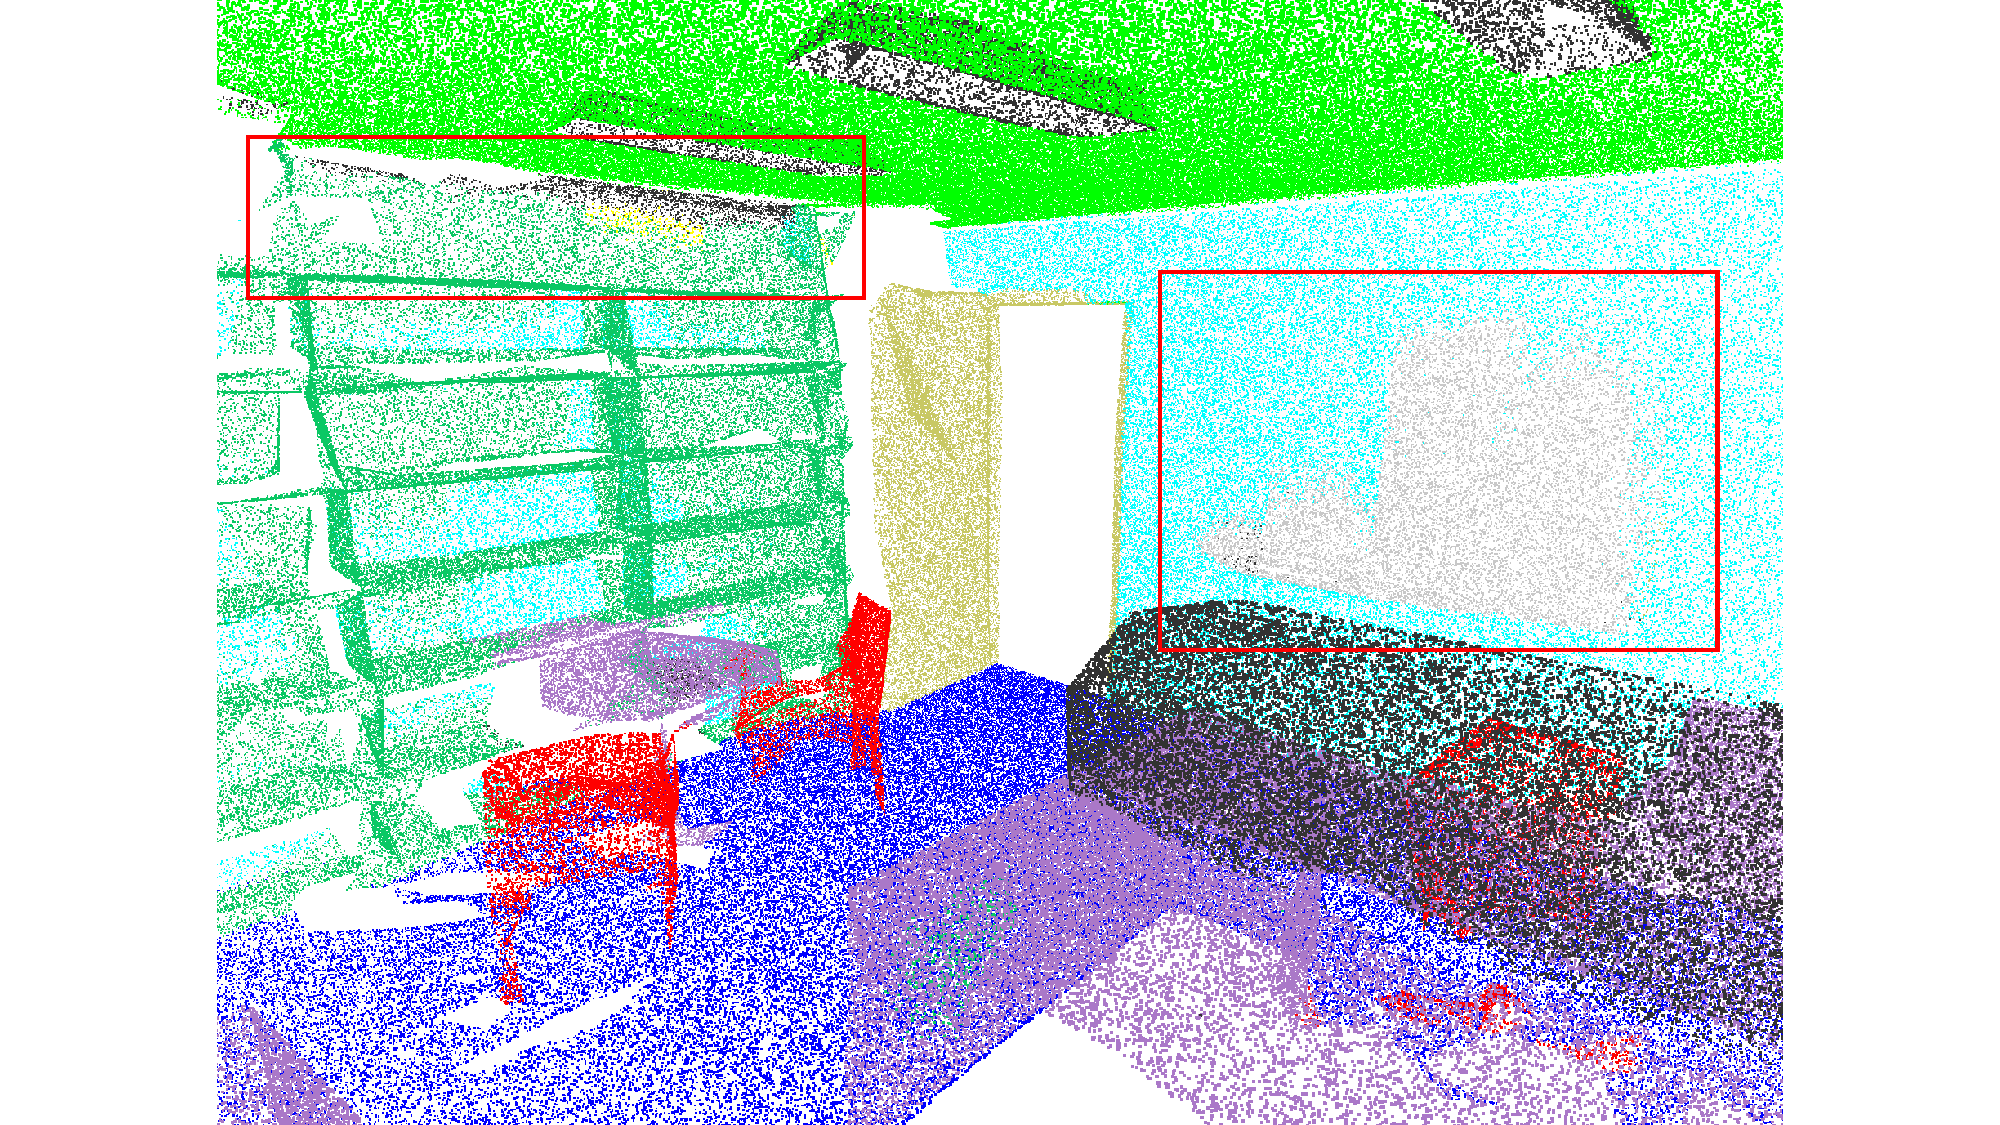
\includegraphics[width=\textwidth]{fig/supplement/semantic_segmentation/office_35/PPT_office_35.pdf}
    \end{minipage}
    \hfill
    \begin{minipage}{0.22\textwidth}
        \centering
        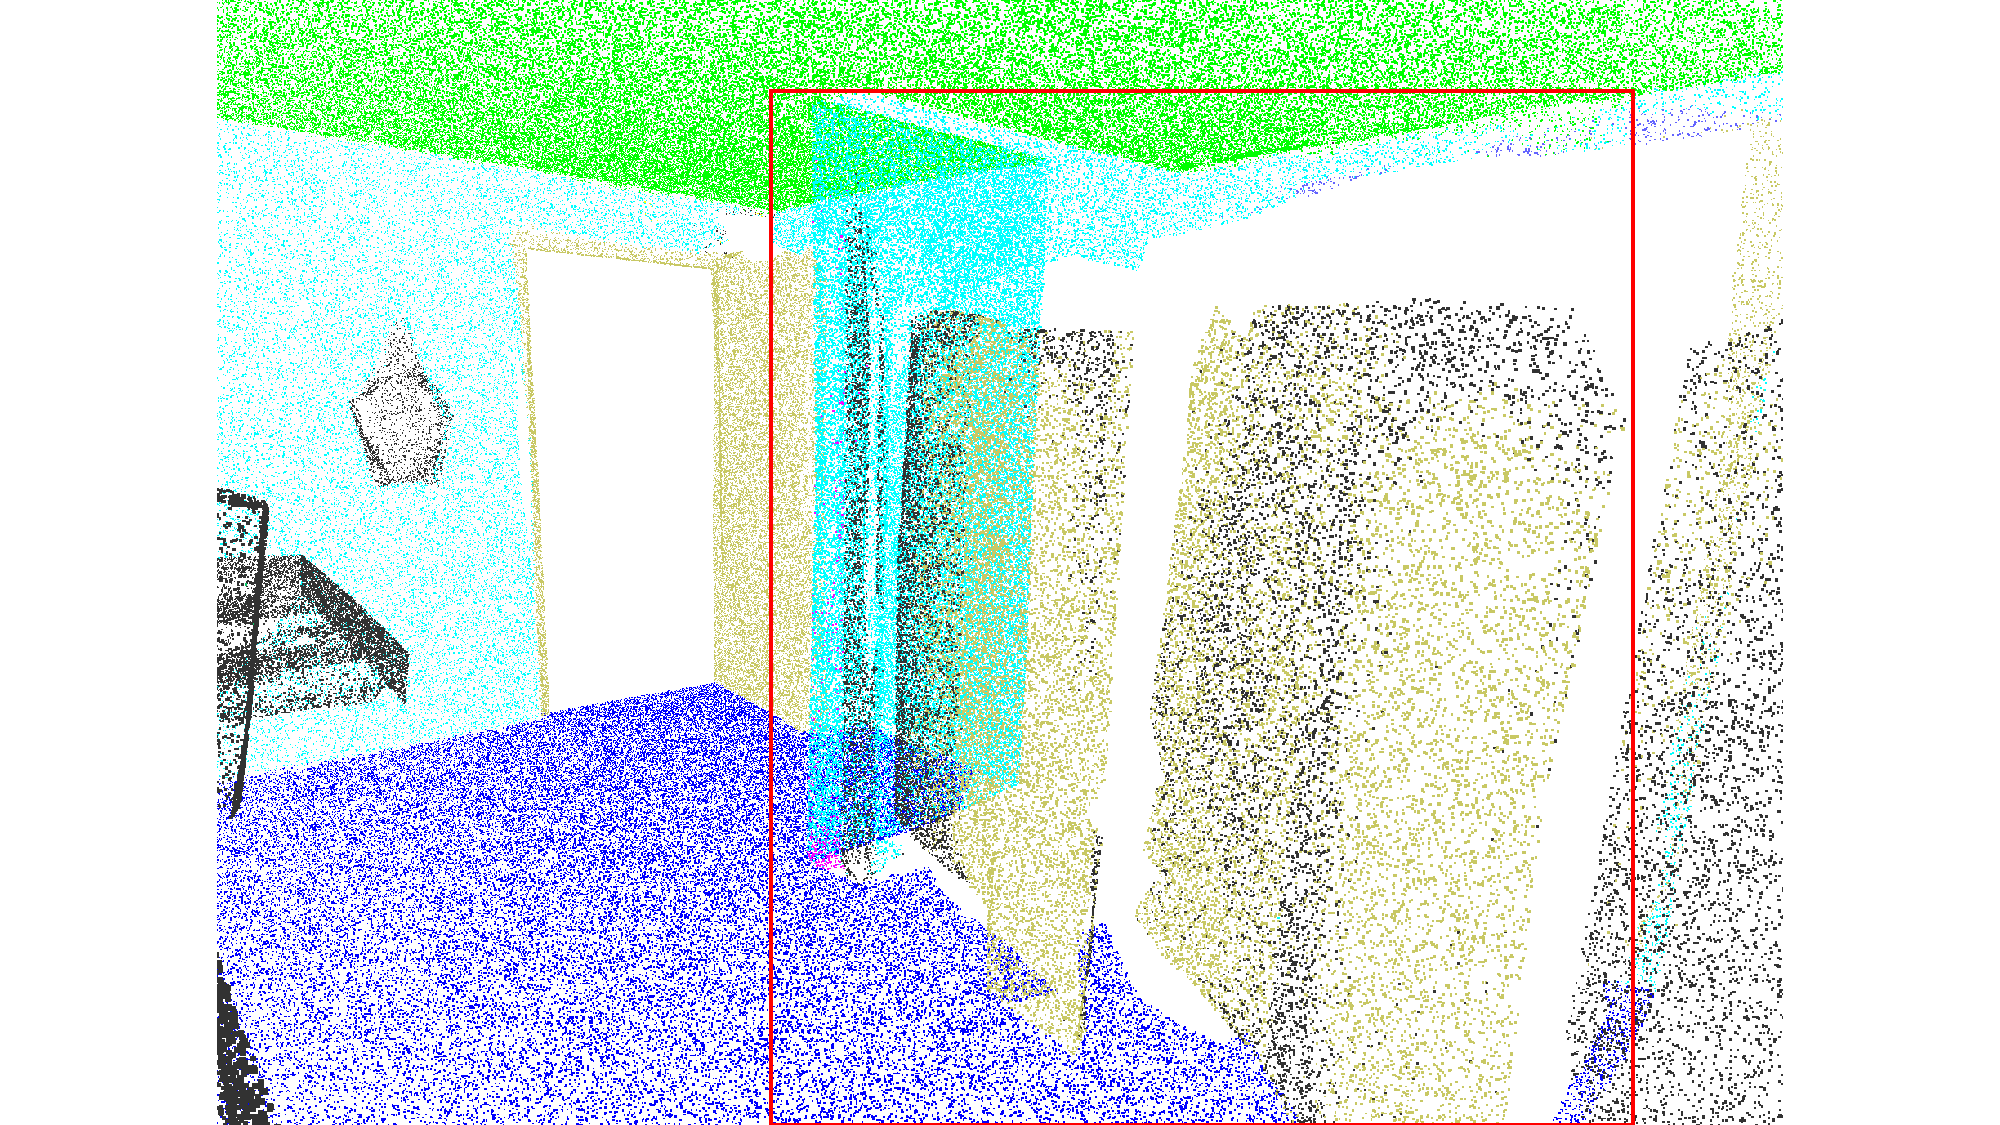
\includegraphics[width=\textwidth]{fig/supplement/semantic_segmentation/wc_2/PPT_wc_2.pdf}
    \end{minipage}
    \hfill

    % 换行
    \vspace{0.5em}

    % 第五行左侧的竖排标签
    \begin{minipage}{0.09\textwidth}
        \centering
        PointGST
    \end{minipage}
    \hfill
    % 第五行图片
    \begin{minipage}{0.22\textwidth}
        \centering
        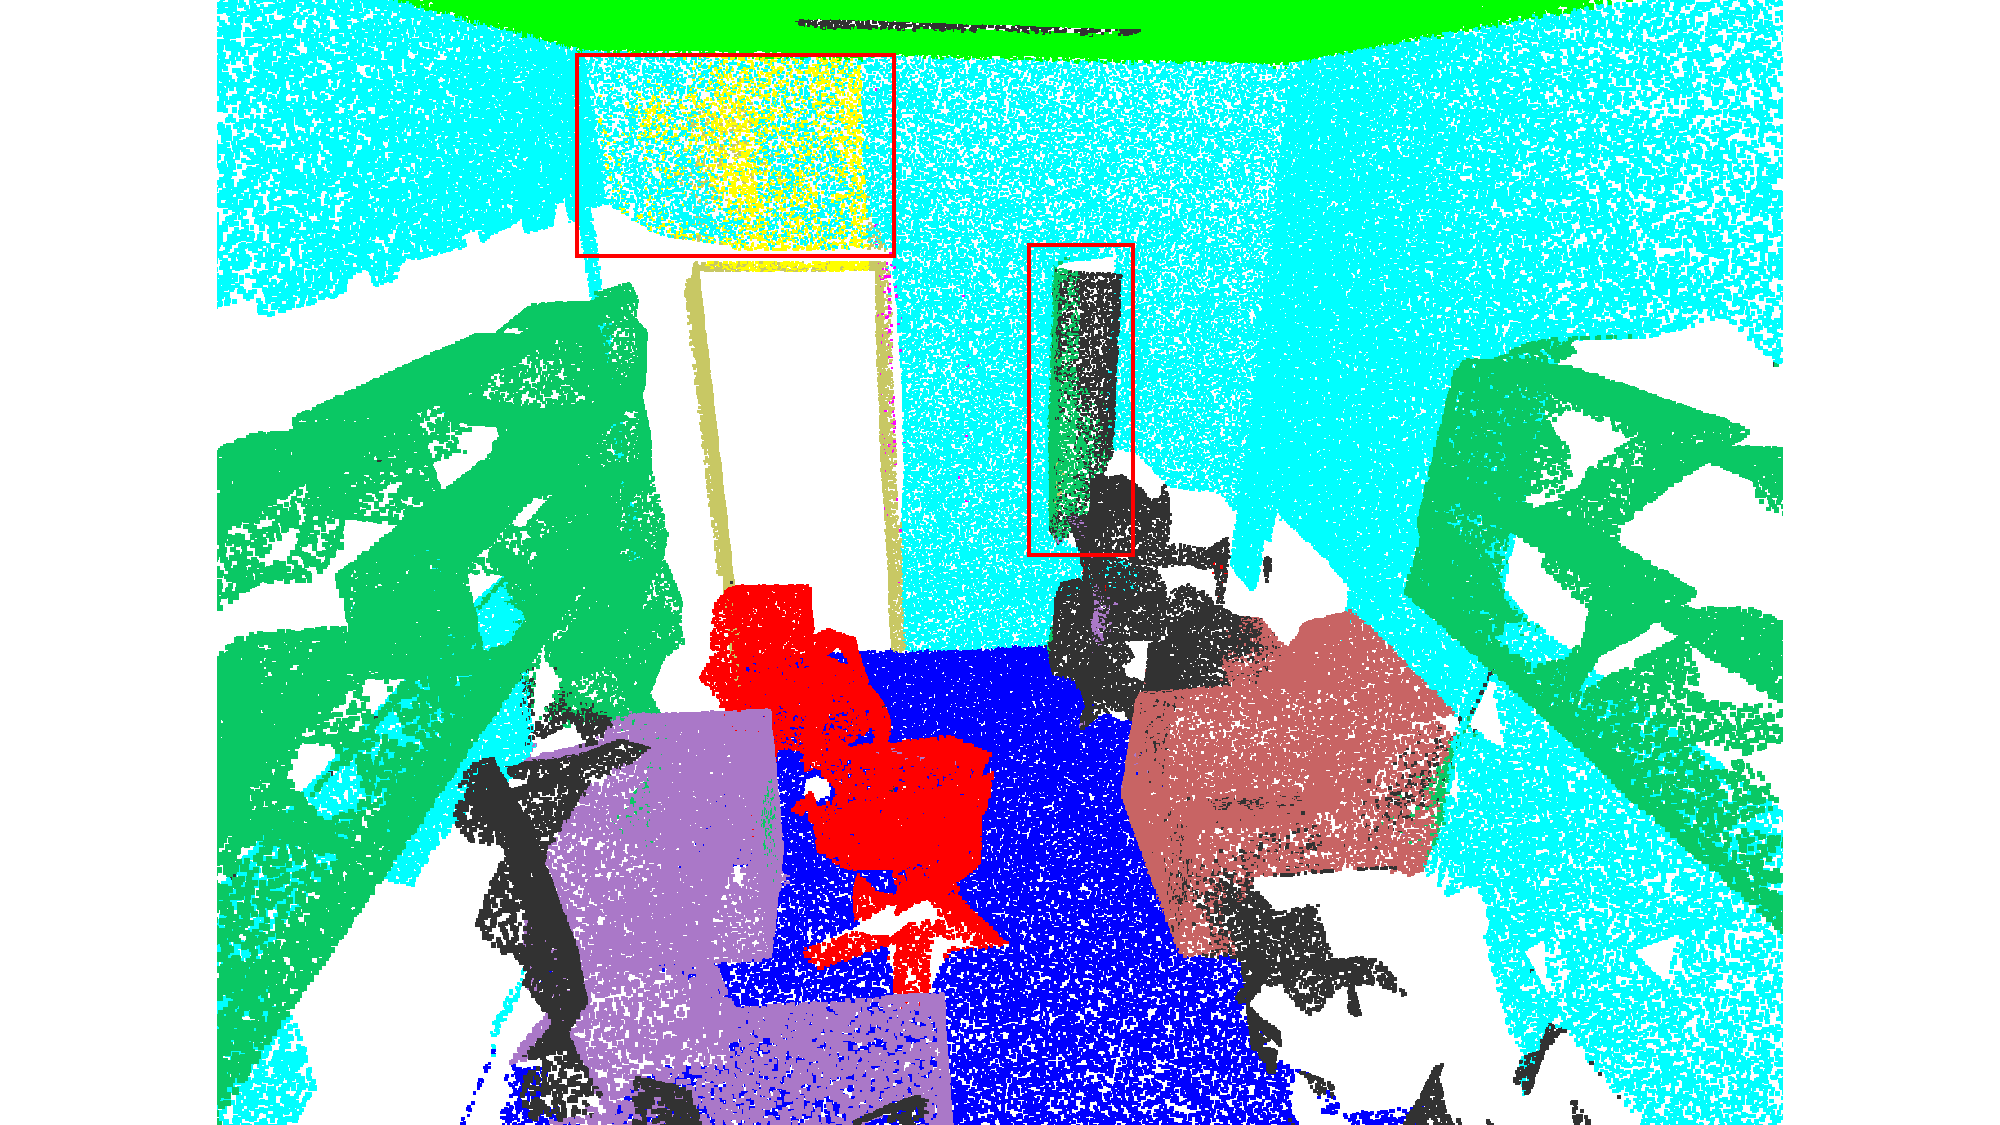
\includegraphics[width=\textwidth]{fig/supplement/semantic_segmentation/office_9/PointGST_office_9.pdf}
    \end{minipage}
    \hfill
    \begin{minipage}{0.22\textwidth}
        \centering
        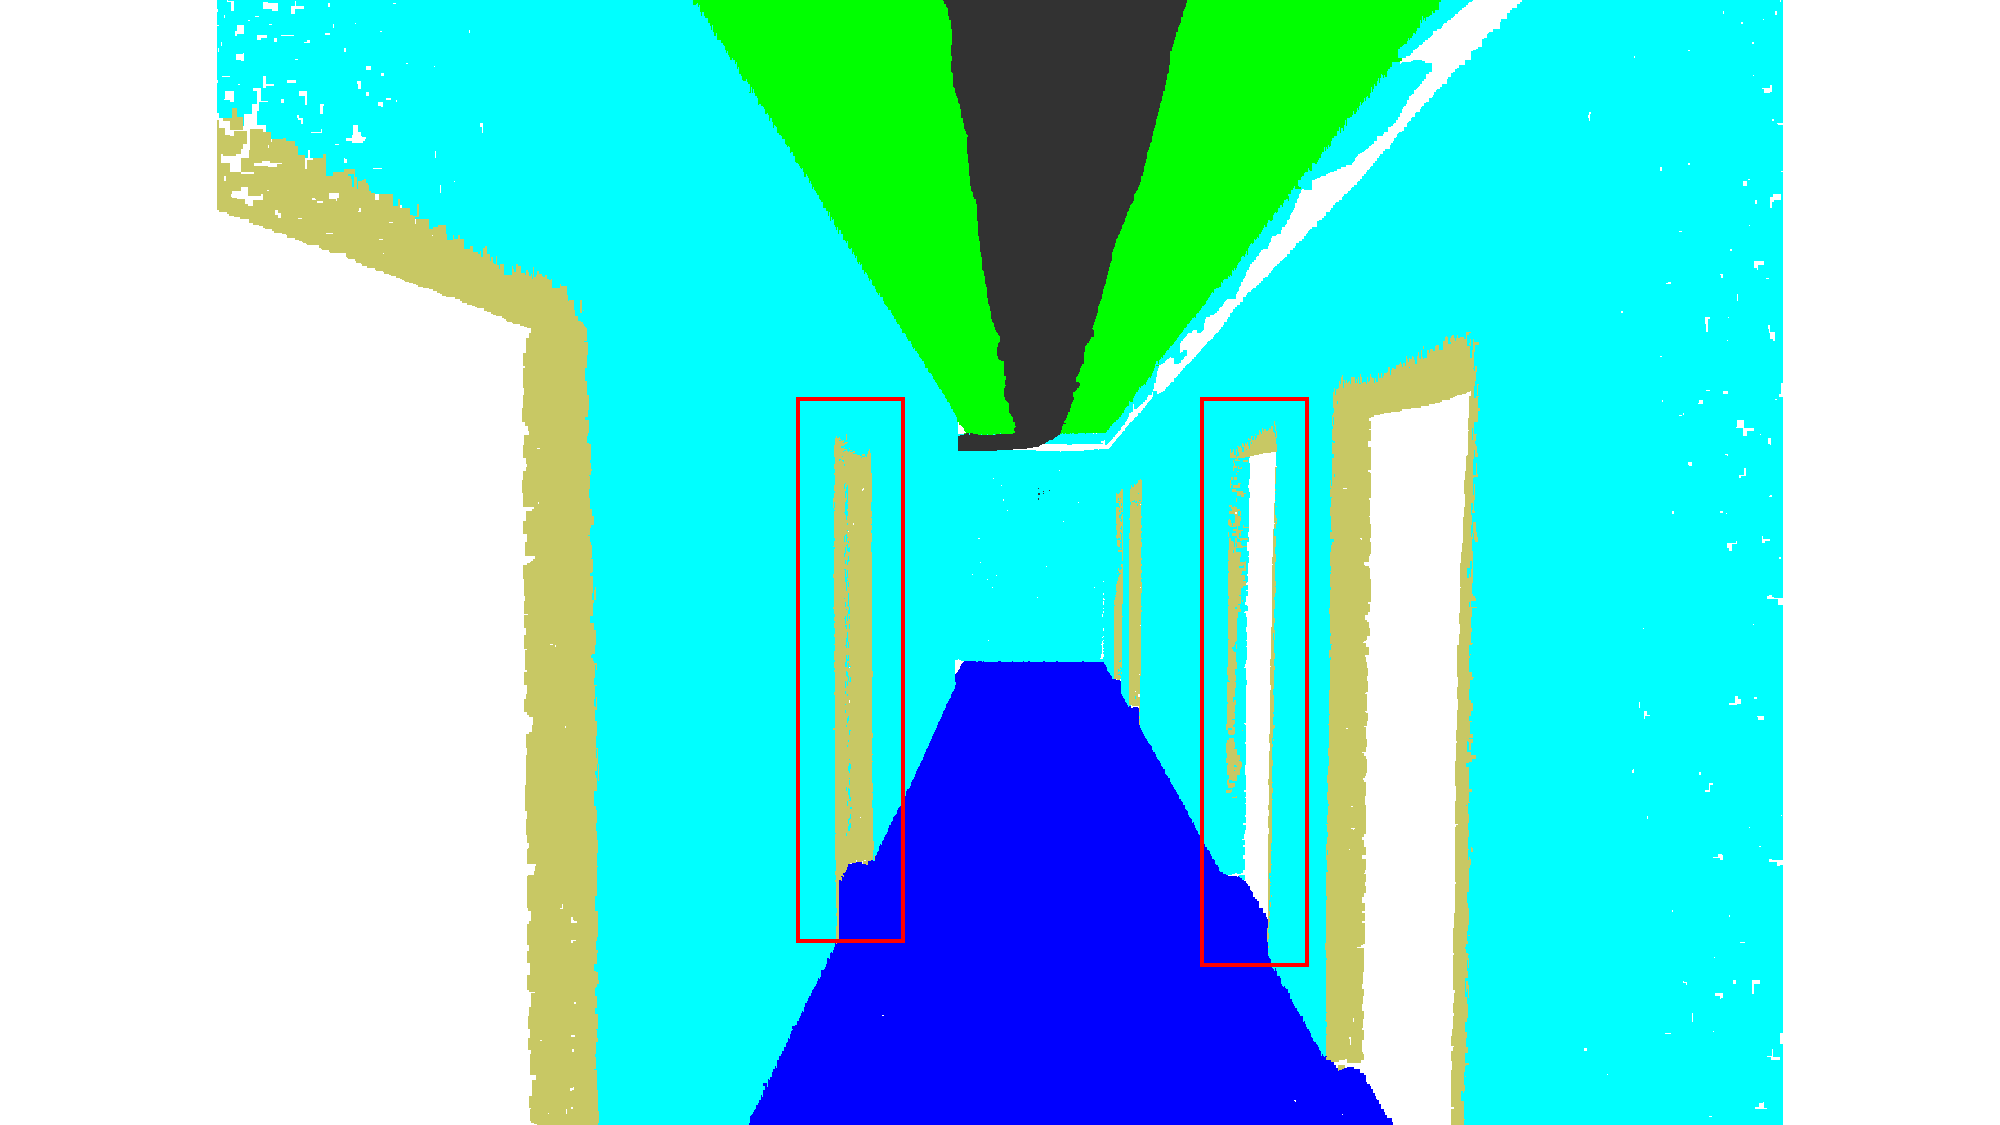
\includegraphics[width=\textwidth]{fig/supplement/semantic_segmentation/hallway_10/PointGST_hallway_10.pdf}
    \end{minipage}
    \hfill
    \begin{minipage}{0.22\textwidth}
        \centering
        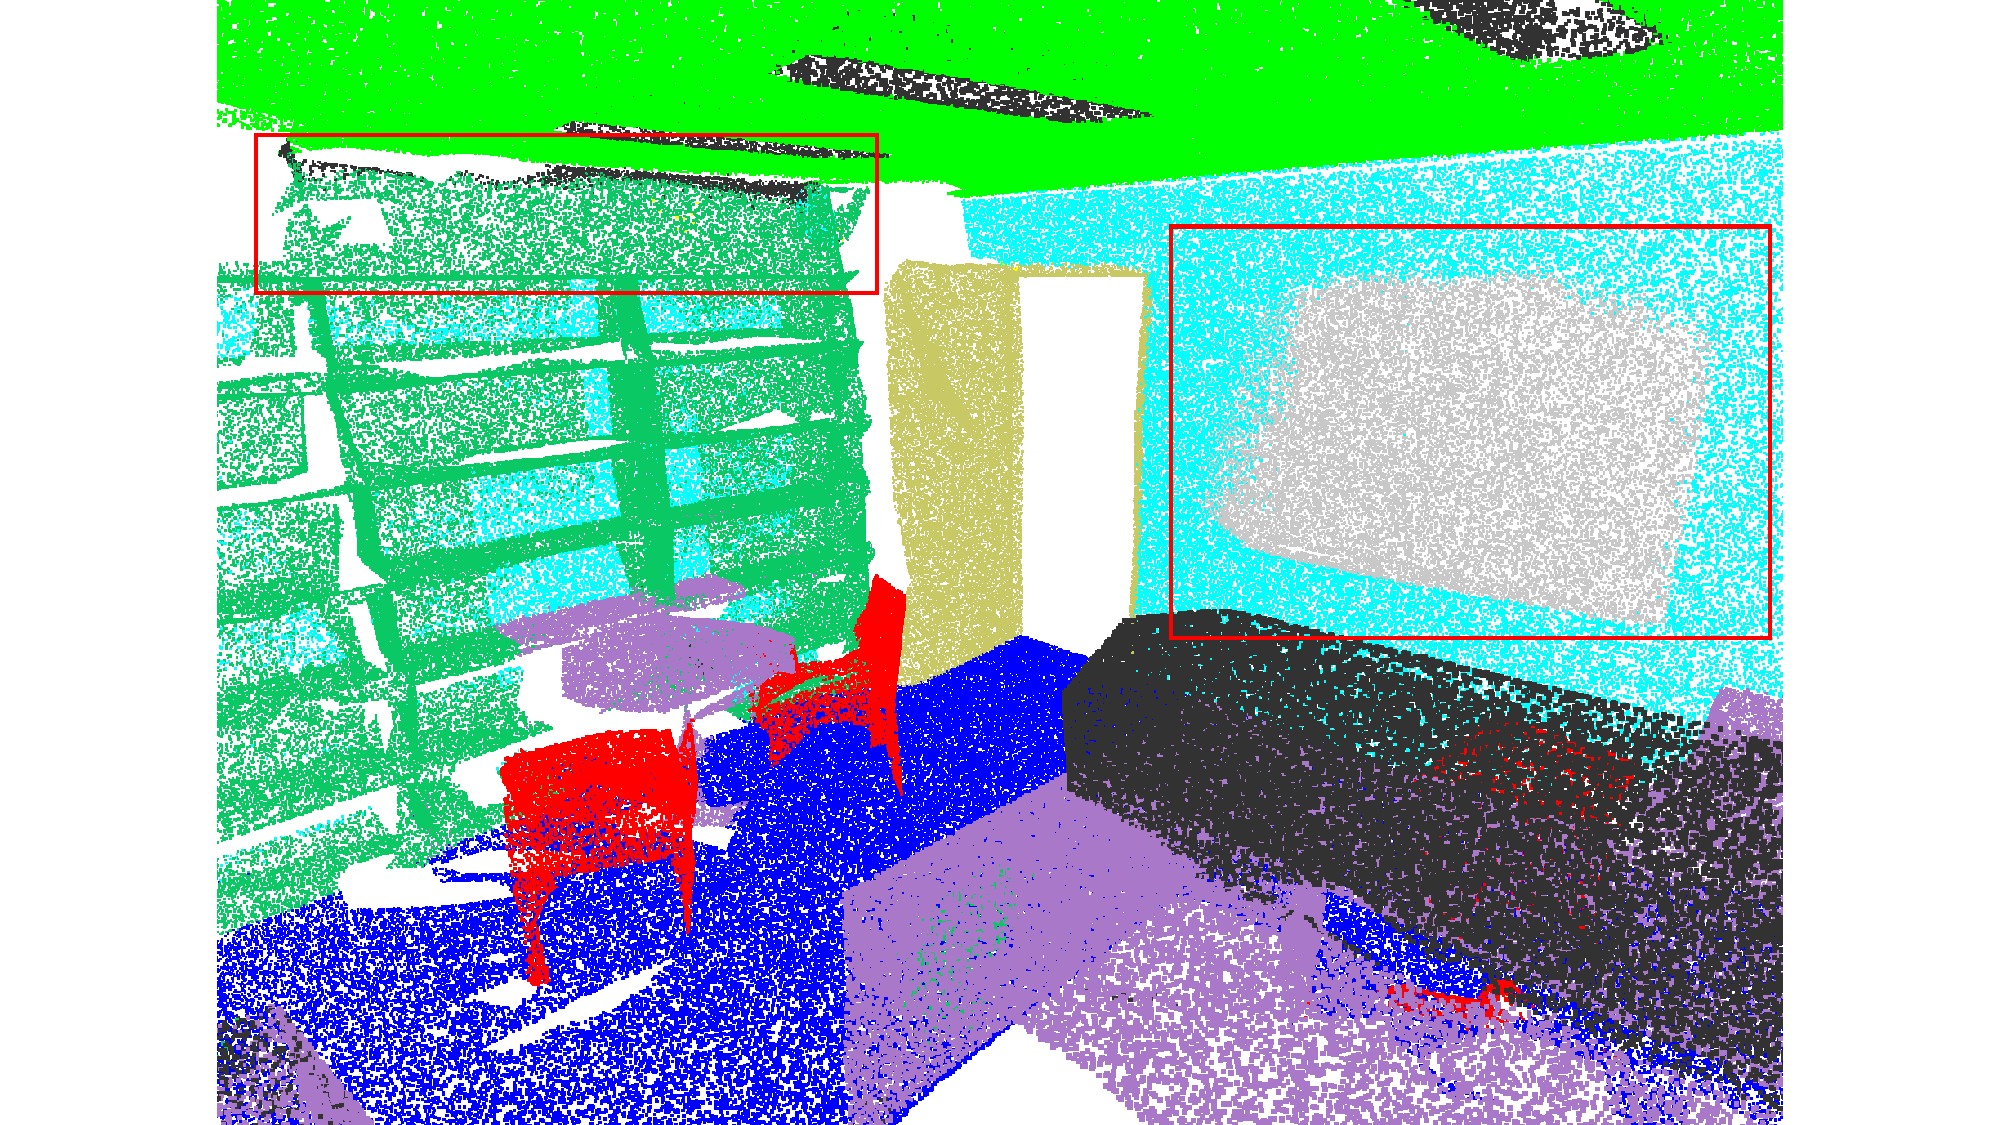
\includegraphics[width=\textwidth]{fig/supplement/semantic_segmentation/office_35/PointGST_office_35.pdf}
    \end{minipage}
    \hfill
    \begin{minipage}{0.22\textwidth}
        \centering
        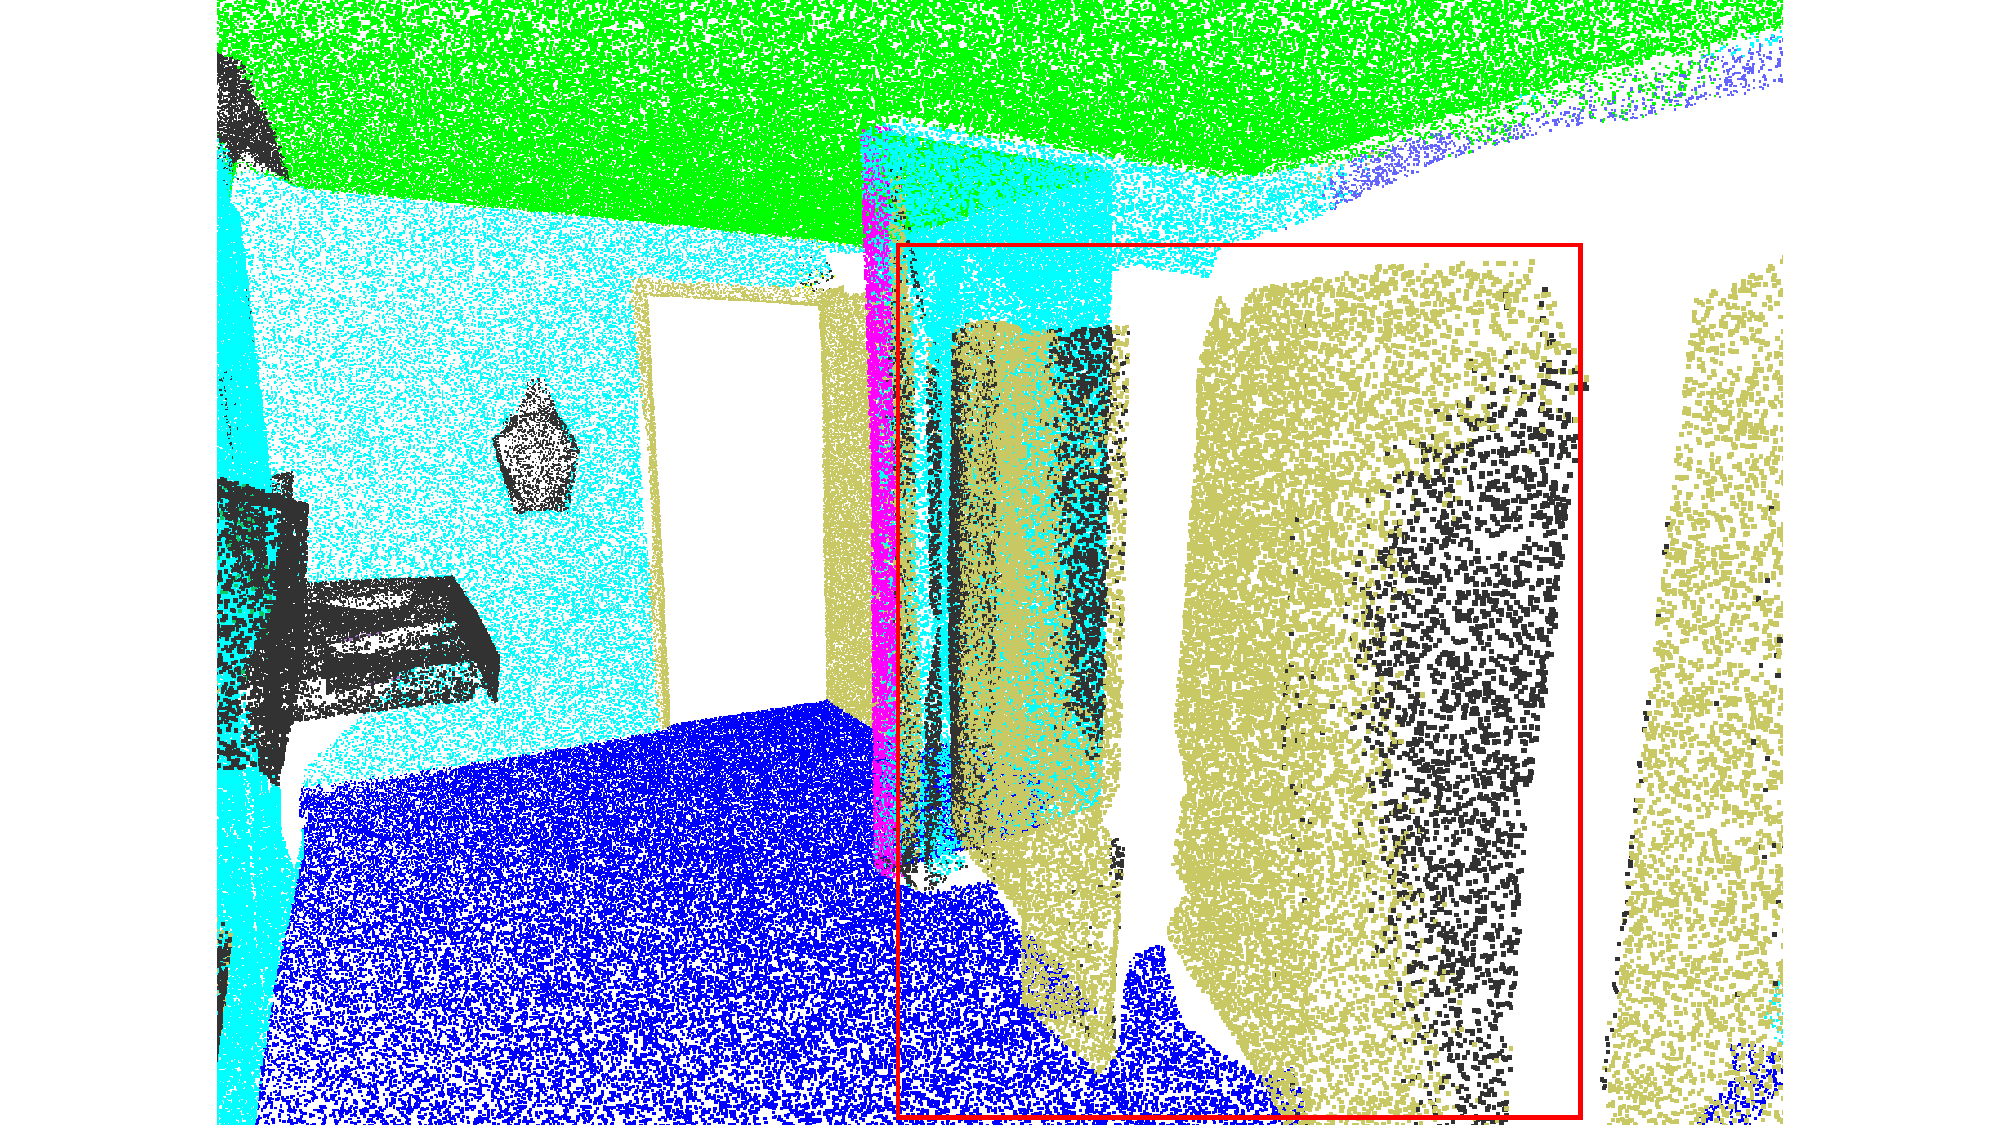
\includegraphics[width=\textwidth]{fig/supplement/semantic_segmentation/wc_2/PointGST_wc_2.pdf}
    \end{minipage}
    \hfill

    % 换行
    \vspace{0.5em}

    % 第六行左侧的竖排标签
    \begin{minipage}{0.09\textwidth}
        \centering
        PLT (Ours)
    \end{minipage}
    \hfill
    % 第六行图片
    \begin{minipage}{0.22\textwidth}
        \centering
        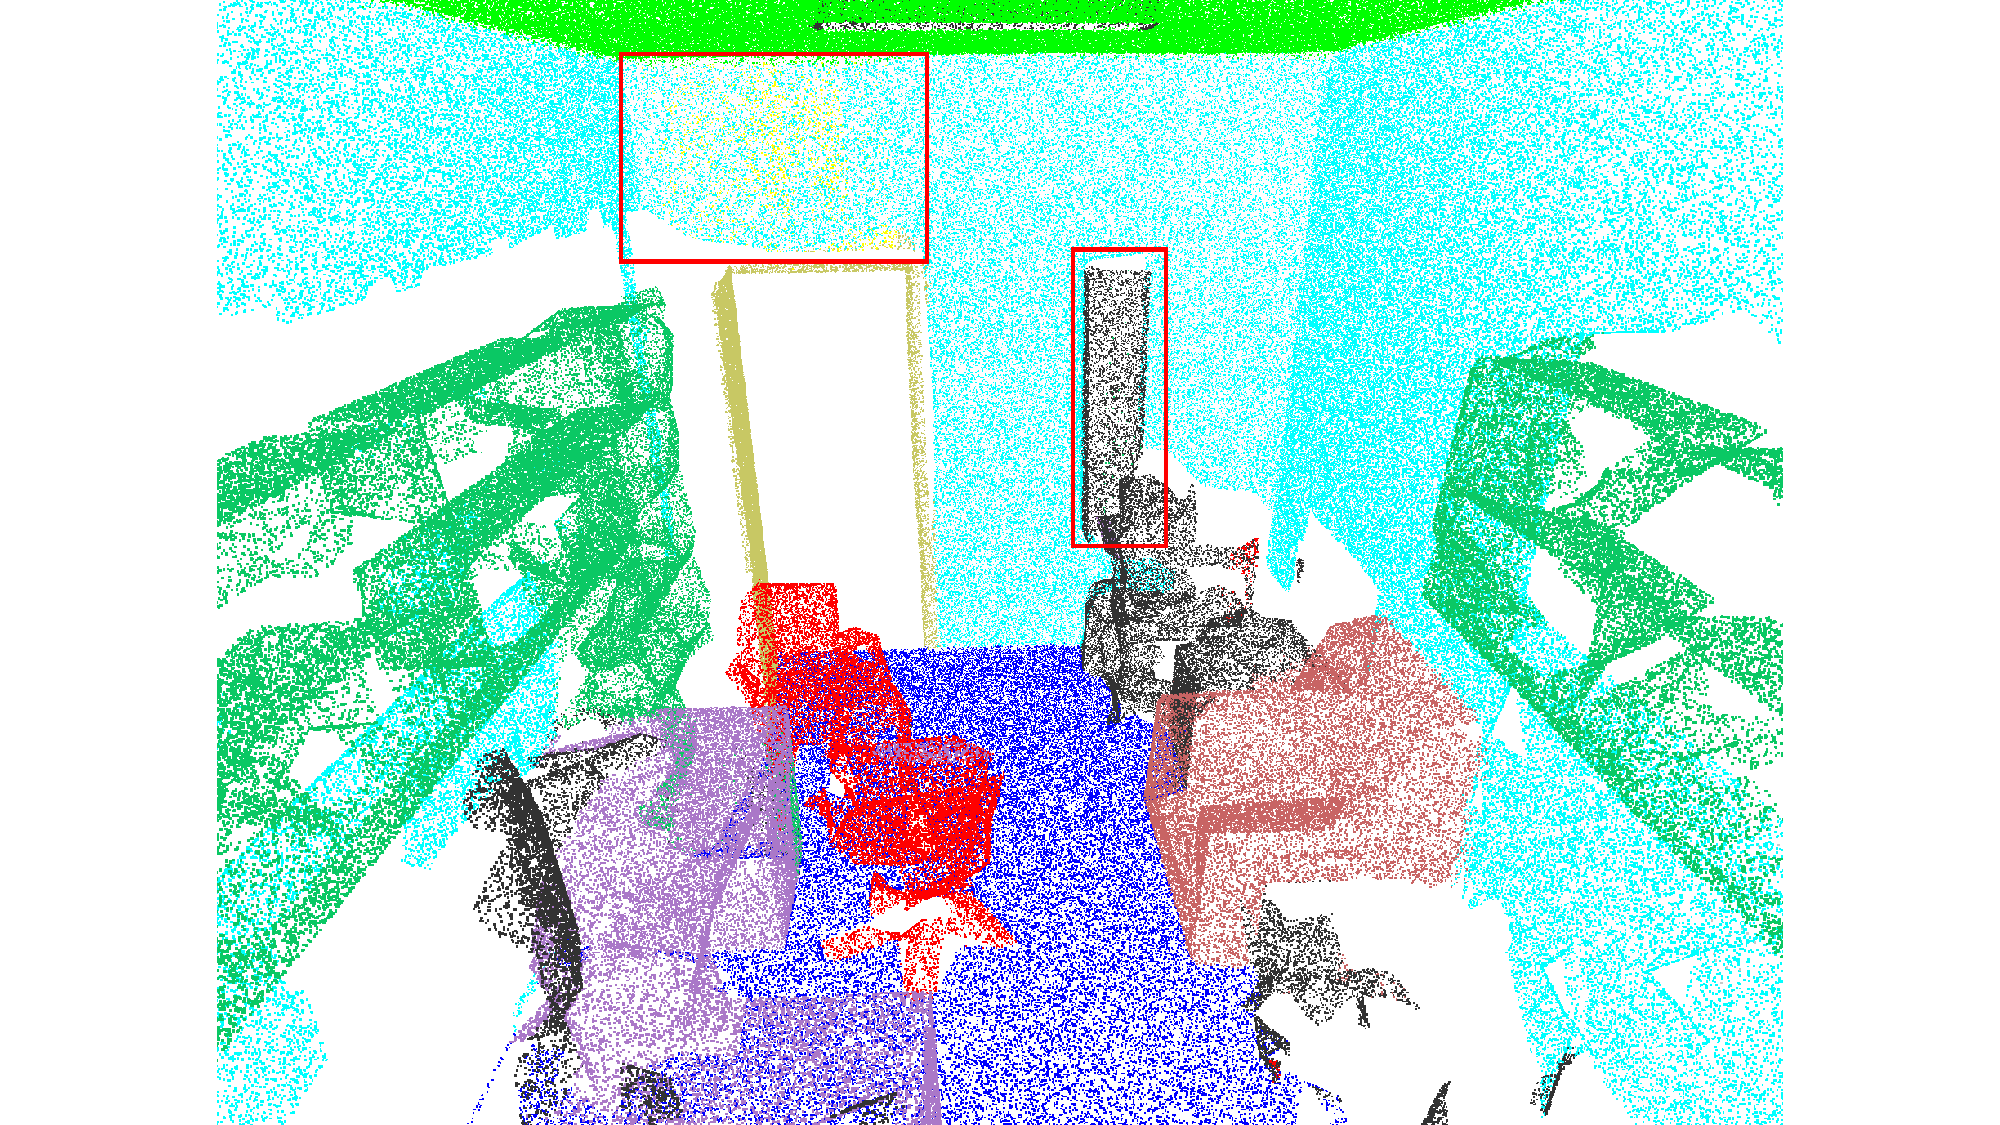
\includegraphics[width=\textwidth]{fig/supplement/semantic_segmentation/office_9/PLT_office_9.pdf}
    \end{minipage}
    \hfill
    \begin{minipage}{0.22\textwidth}
        \centering
        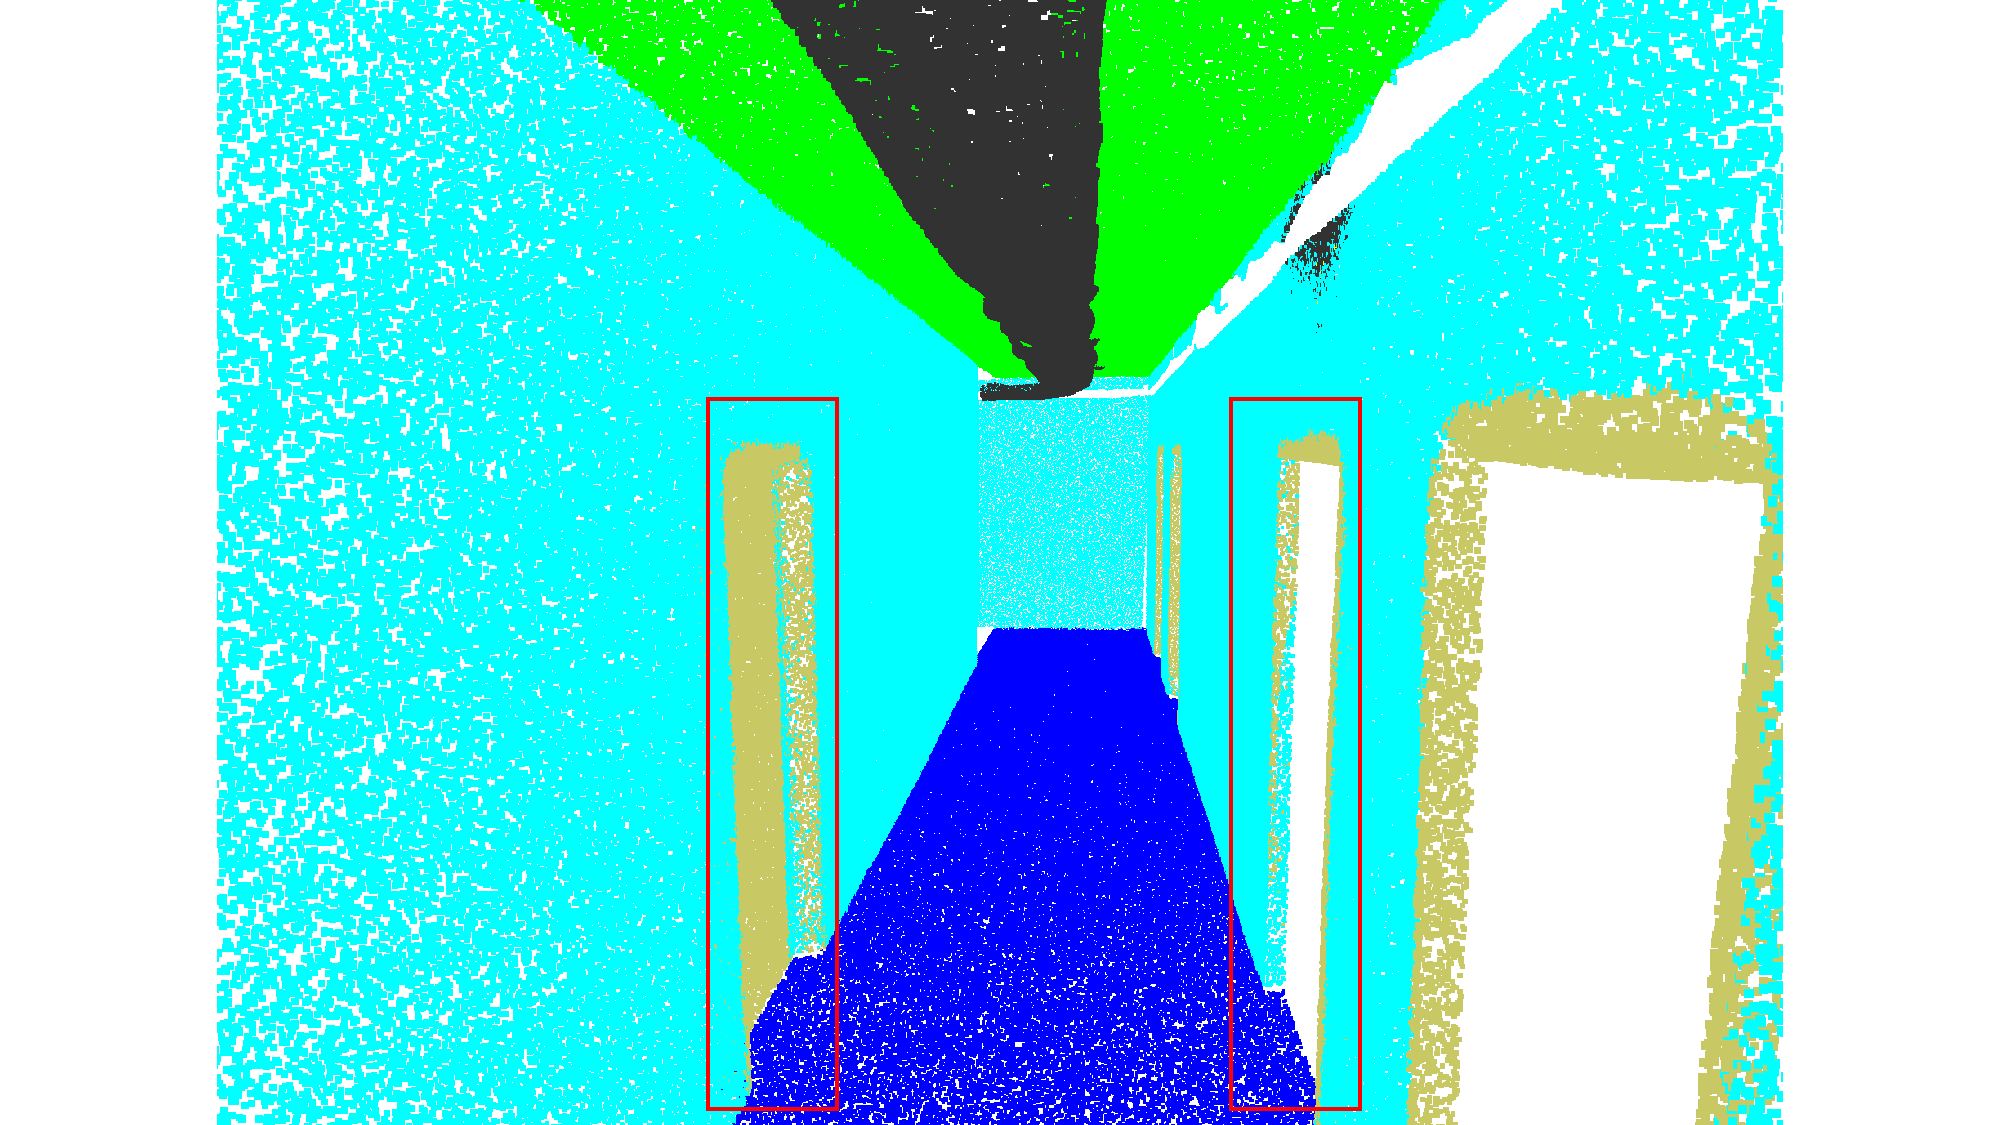
\includegraphics[width=\textwidth]{fig/supplement/semantic_segmentation/hallway_10/PLT_hallway_10.pdf}
    \end{minipage}
    \hfill
    \begin{minipage}{0.22\textwidth}
        \centering
        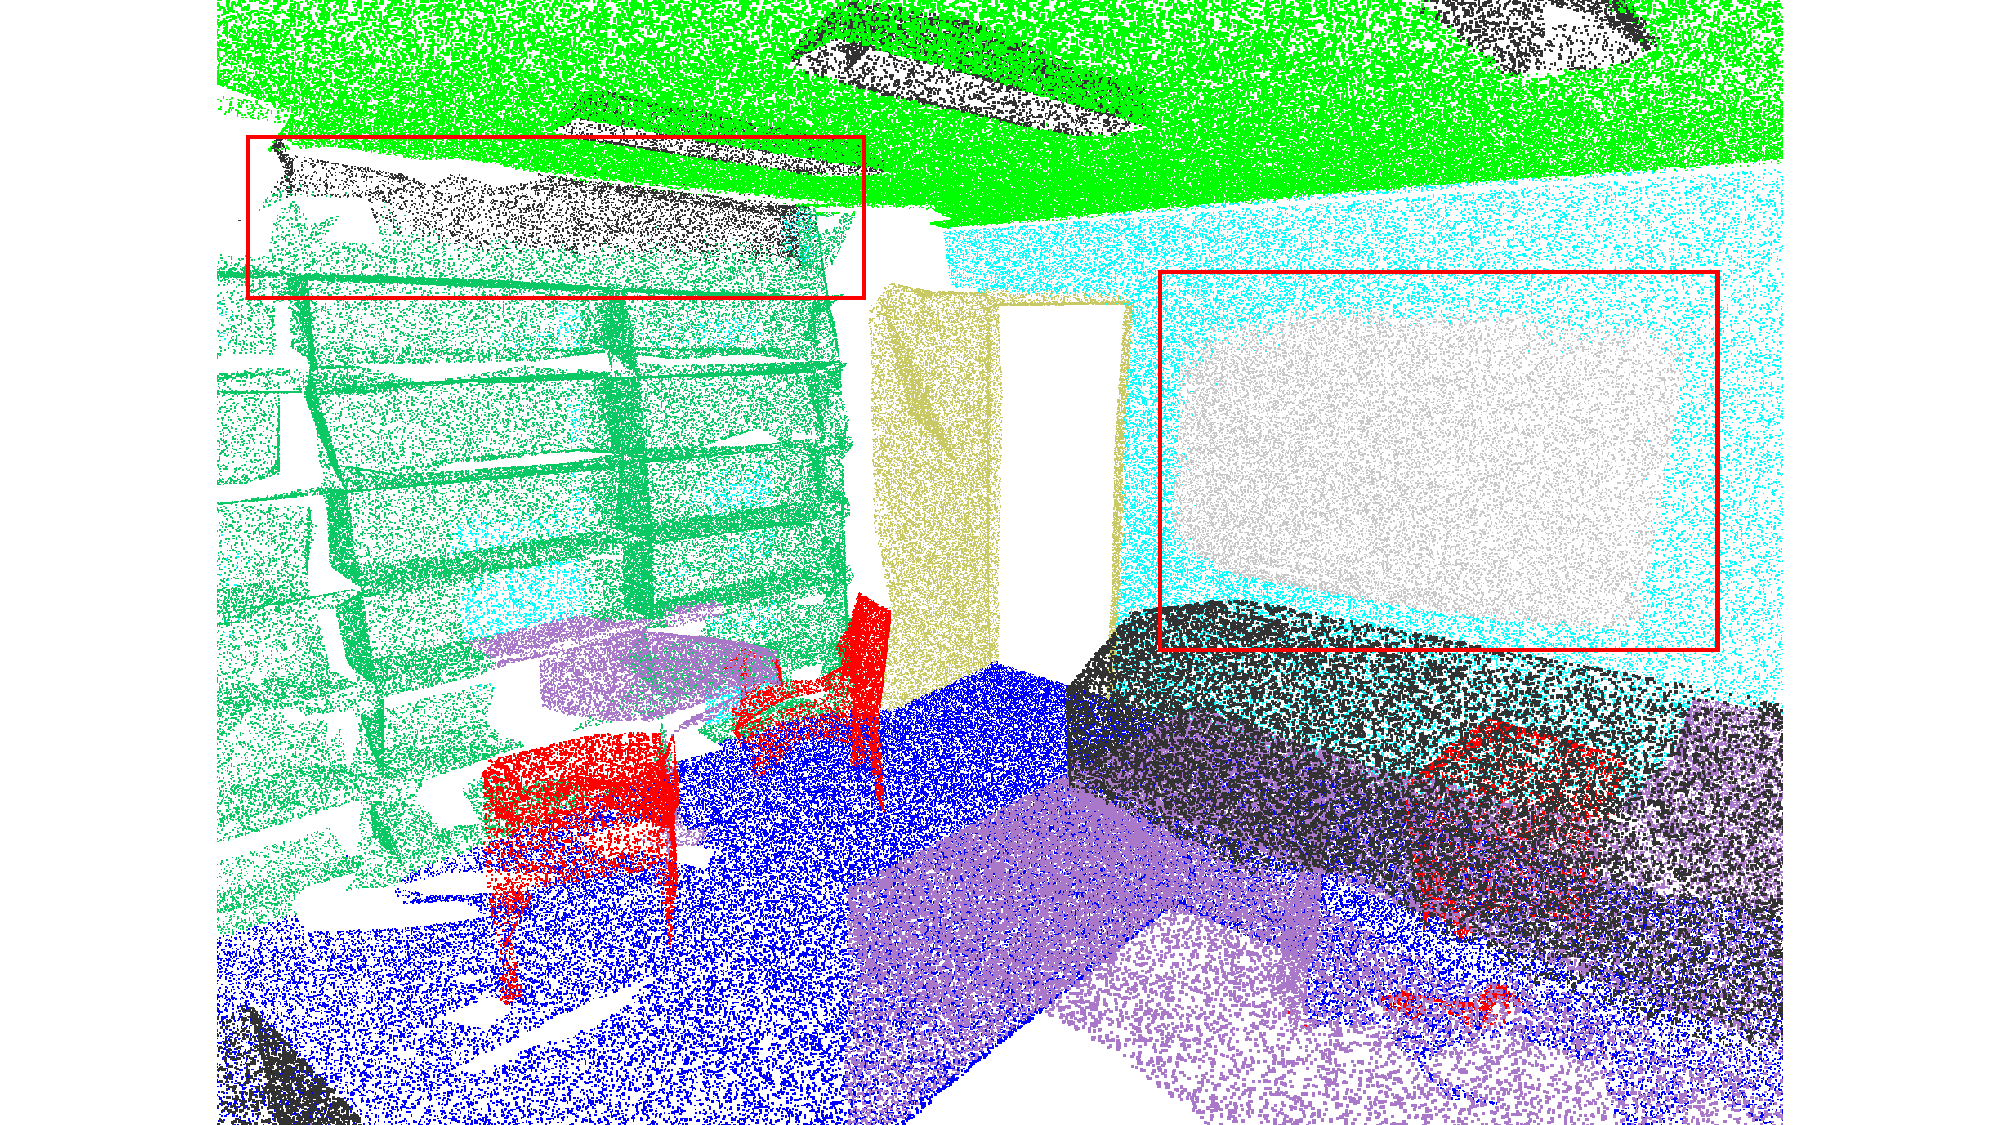
\includegraphics[width=\textwidth]{fig/supplement/semantic_segmentation/office_35/PLT_office_35.pdf}
    \end{minipage}
    \hfill
    \begin{minipage}{0.22\textwidth}
        \centering
        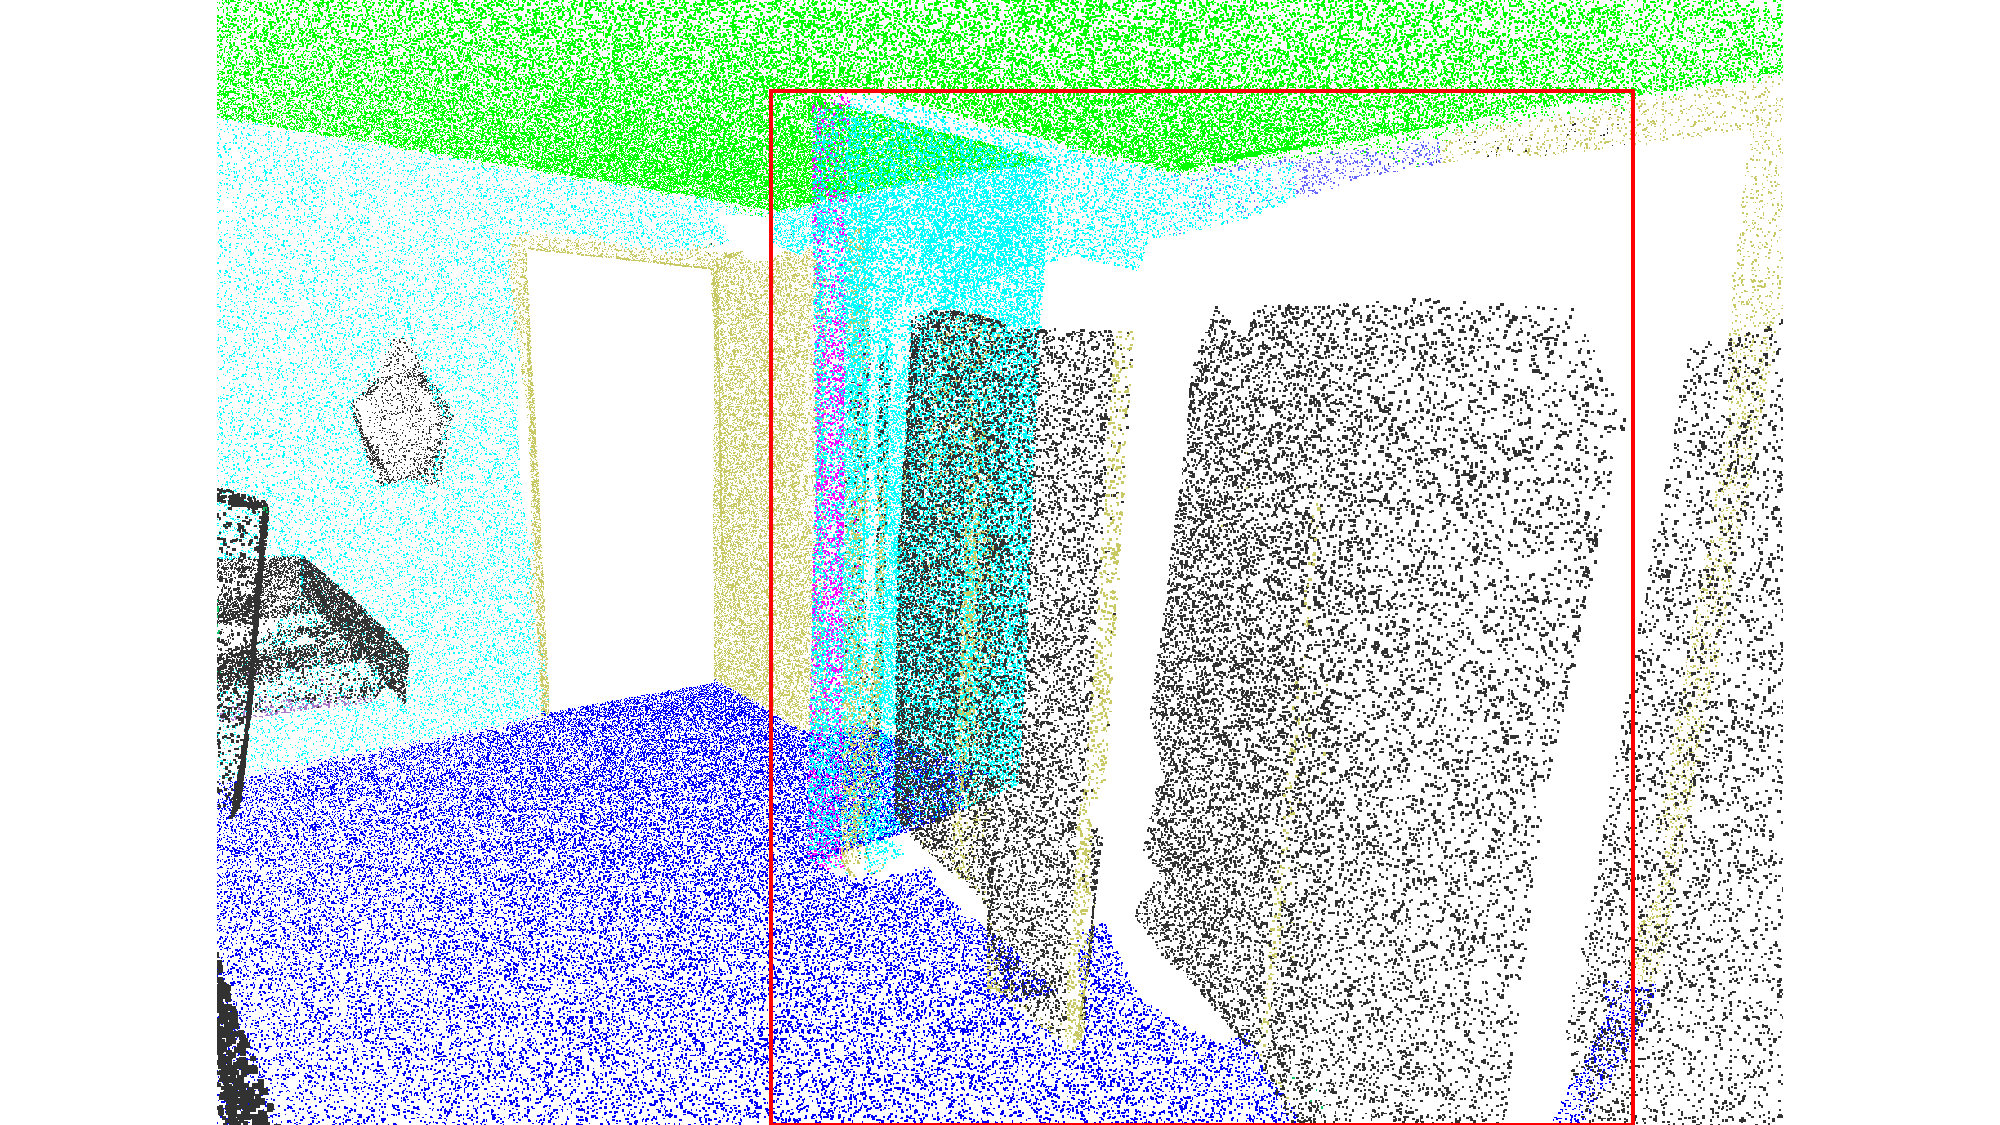
\includegraphics[width=\textwidth]{fig/supplement/semantic_segmentation/wc_2/PLT_wc_2.pdf}
    \end{minipage}
    \hfill

    % 换行
    \vspace{0.5em}

    % 第七行左侧的竖排标签
    \begin{minipage}{0.09\textwidth}
        \centering
        GT
    \end{minipage}
    \hfill
    % 第七行图片
    \begin{minipage}{0.22\textwidth}
        \centering
        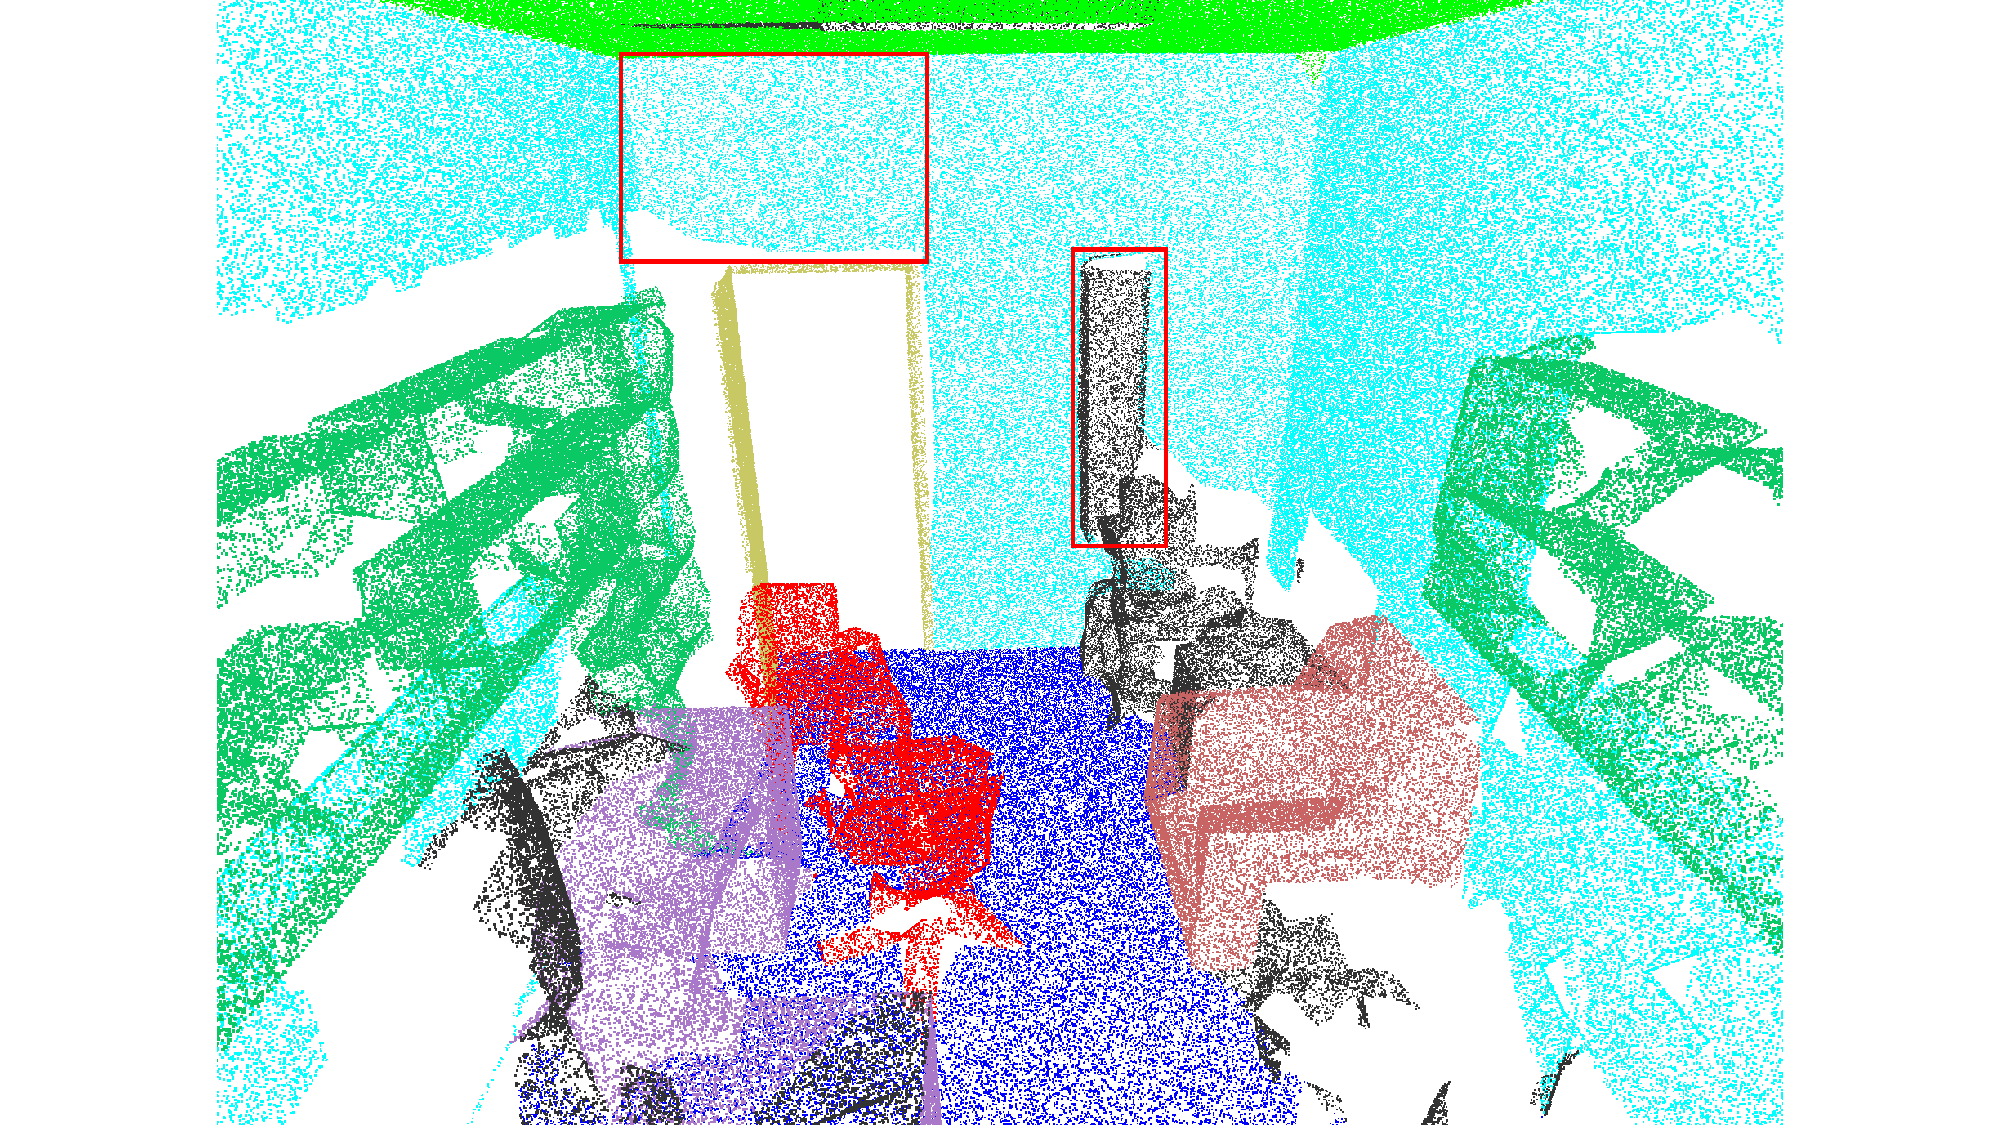
\includegraphics[width=\textwidth]{fig/supplement/semantic_segmentation/office_9/GT_office_9.pdf}
    \end{minipage}
    \hfill
    \begin{minipage}{0.22\textwidth}
        \centering
        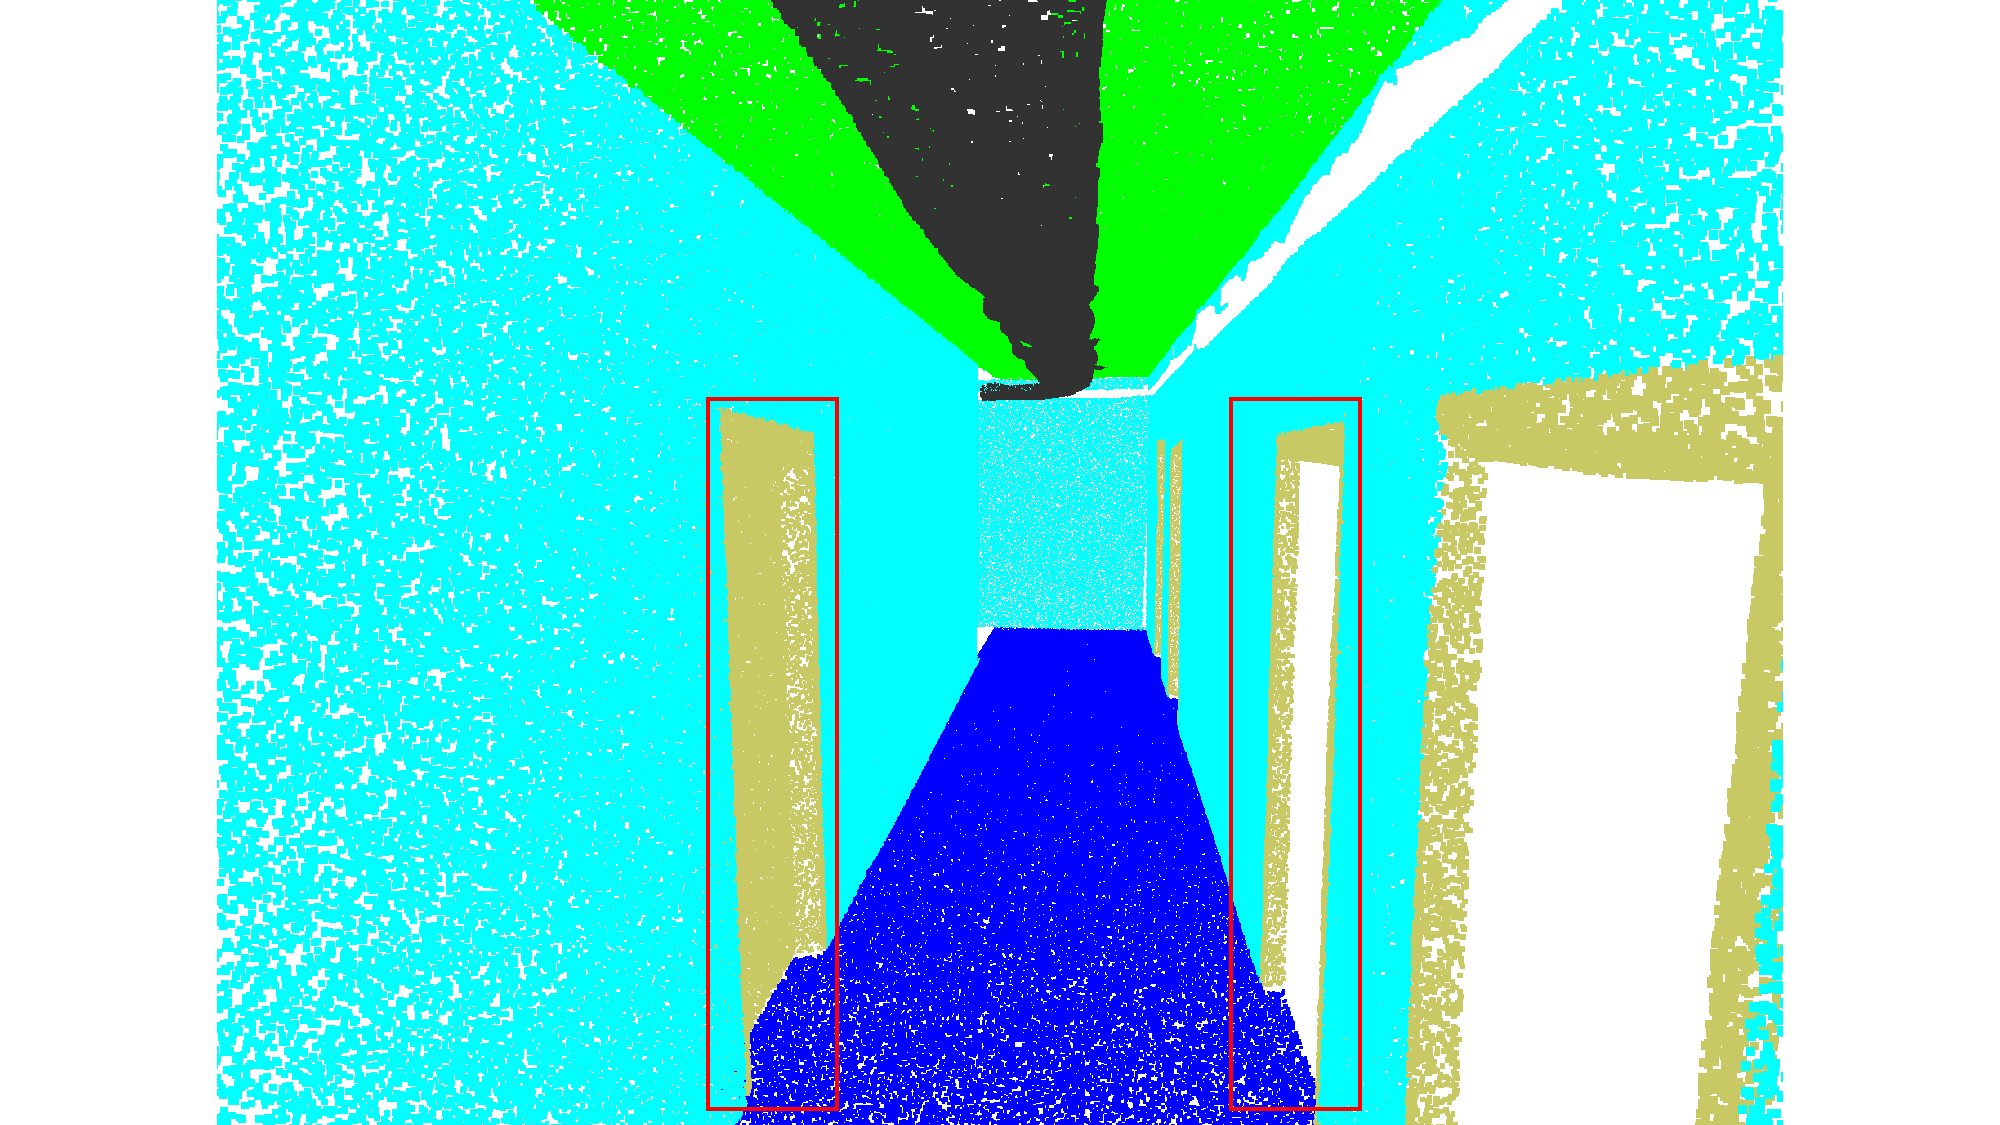
\includegraphics[width=\textwidth]{fig/supplement/semantic_segmentation/hallway_10/GT_hallway_10.pdf}
    \end{minipage}
    \hfill
    \begin{minipage}{0.22\textwidth}
        \centering
        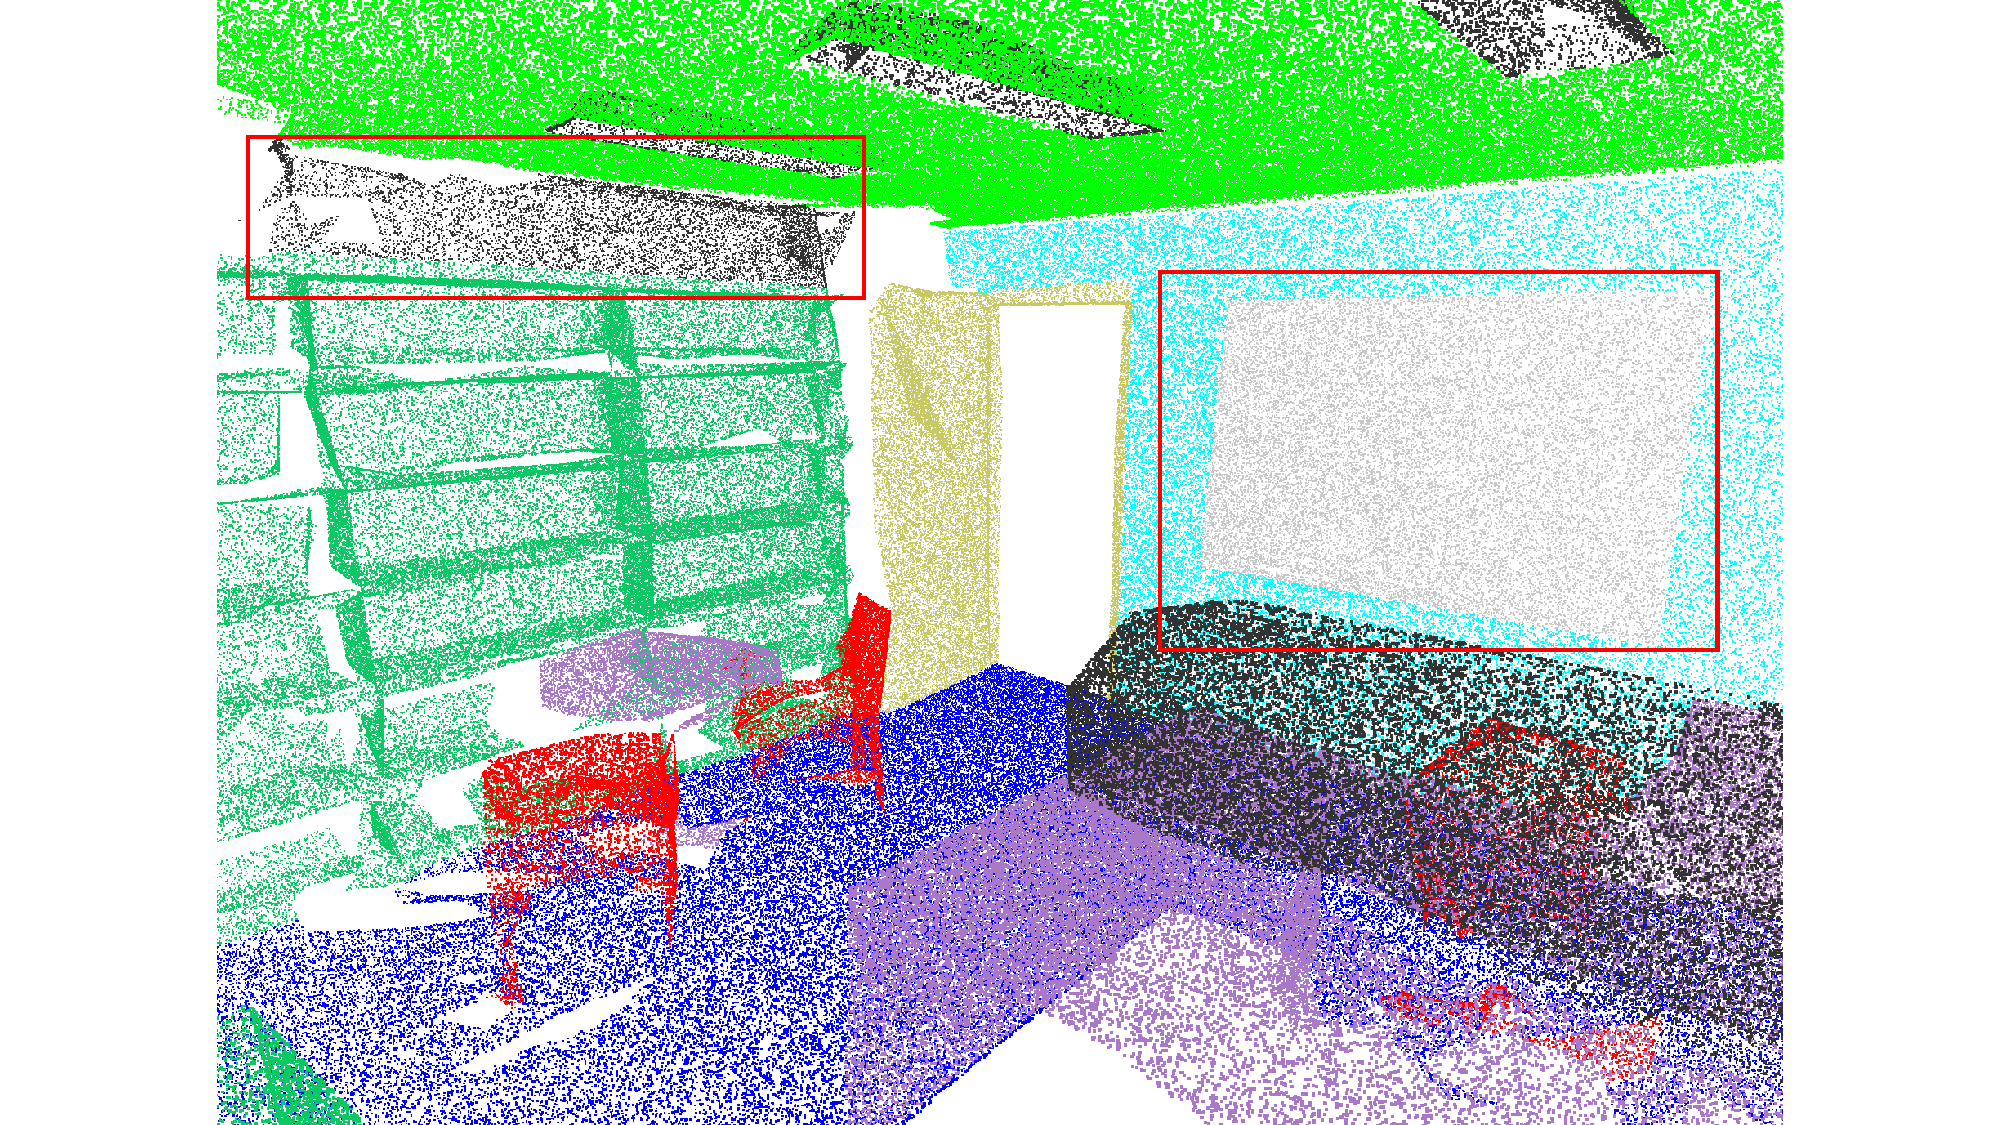
\includegraphics[width=\textwidth]{fig/supplement/semantic_segmentation/office_35/GT_office_35.pdf}
    \end{minipage}
    \hfill
    \begin{minipage}{0.22\textwidth}
        \centering
        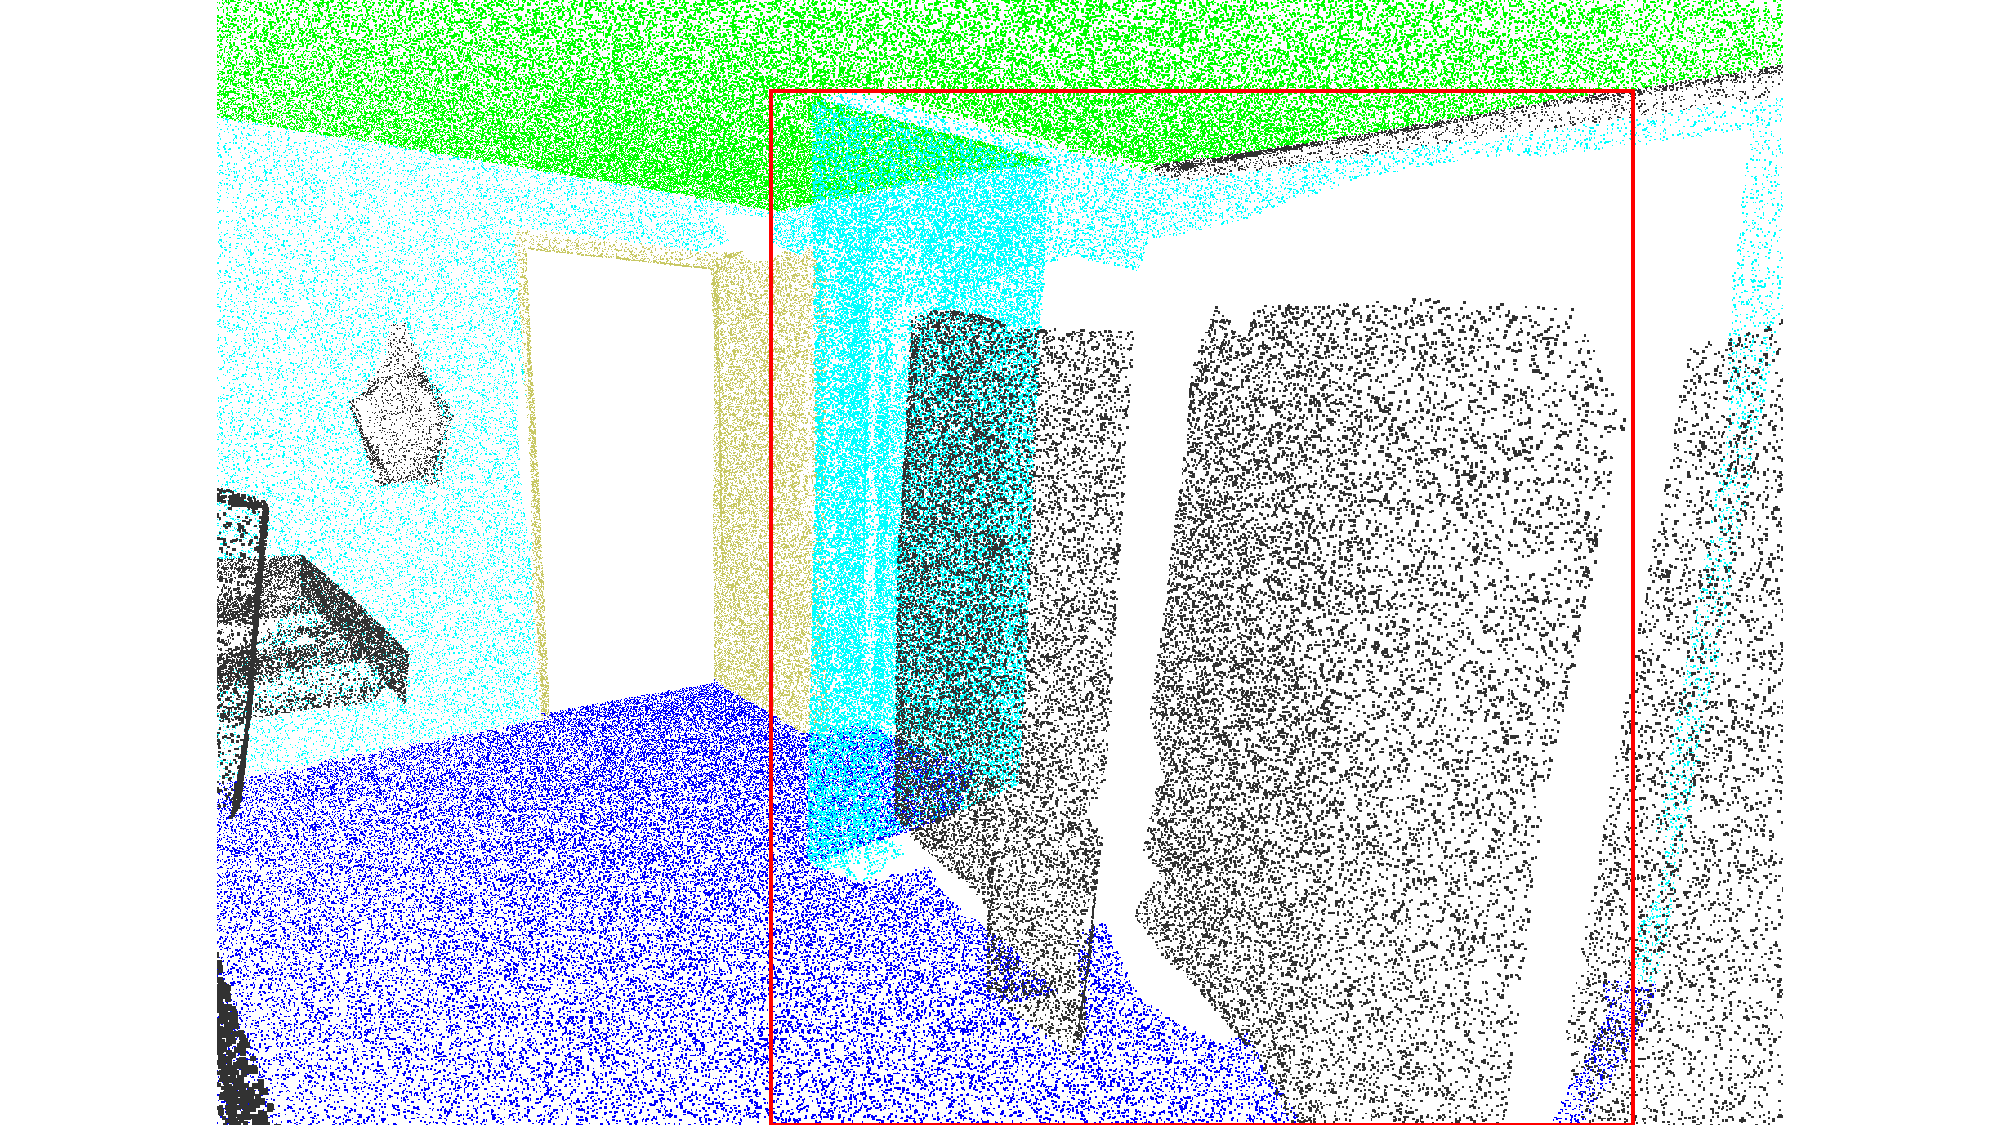
\includegraphics[width=\textwidth]{fig/supplement/semantic_segmentation/wc_2/GT_wc_2.pdf}
    \end{minipage}
    \hfill
    
    %下方的标签
    \vspace{0.5em}
    \begin{minipage}{0.09\textwidth} % 左侧空白区域
        \color{white}{12}
    \end{minipage}
    \hfill
    \begin{minipage}{0.22\textwidth} % 第2列标题
        \centering
        office\_9
    \end{minipage}
    \hfill
    \begin{minipage}{0.22\textwidth} % 第1列标题
        \centering
        hallway\_10
    \end{minipage}
    \hfill
    \begin{minipage}{0.22\textwidth} % 第3列标题
        \centering
        office\_35
    \end{minipage}
    \hfill
    \begin{minipage}{0.22\textwidth} % 第3列标题
        \centering
        wc\_2
    \end{minipage}
    \hfill
    \caption{The visualization of qualitative results for point cloud semantic segmentation. We compare our PLT with previous methods on Area 5 of the S3DIS dataset~\cite{armeni20163d}.}
    \label{fig:s3dis_1}

\end{figure*}

\begin{figure*}
    \centering
    \begin{subfigure}{0.19\textwidth}
        \centering
        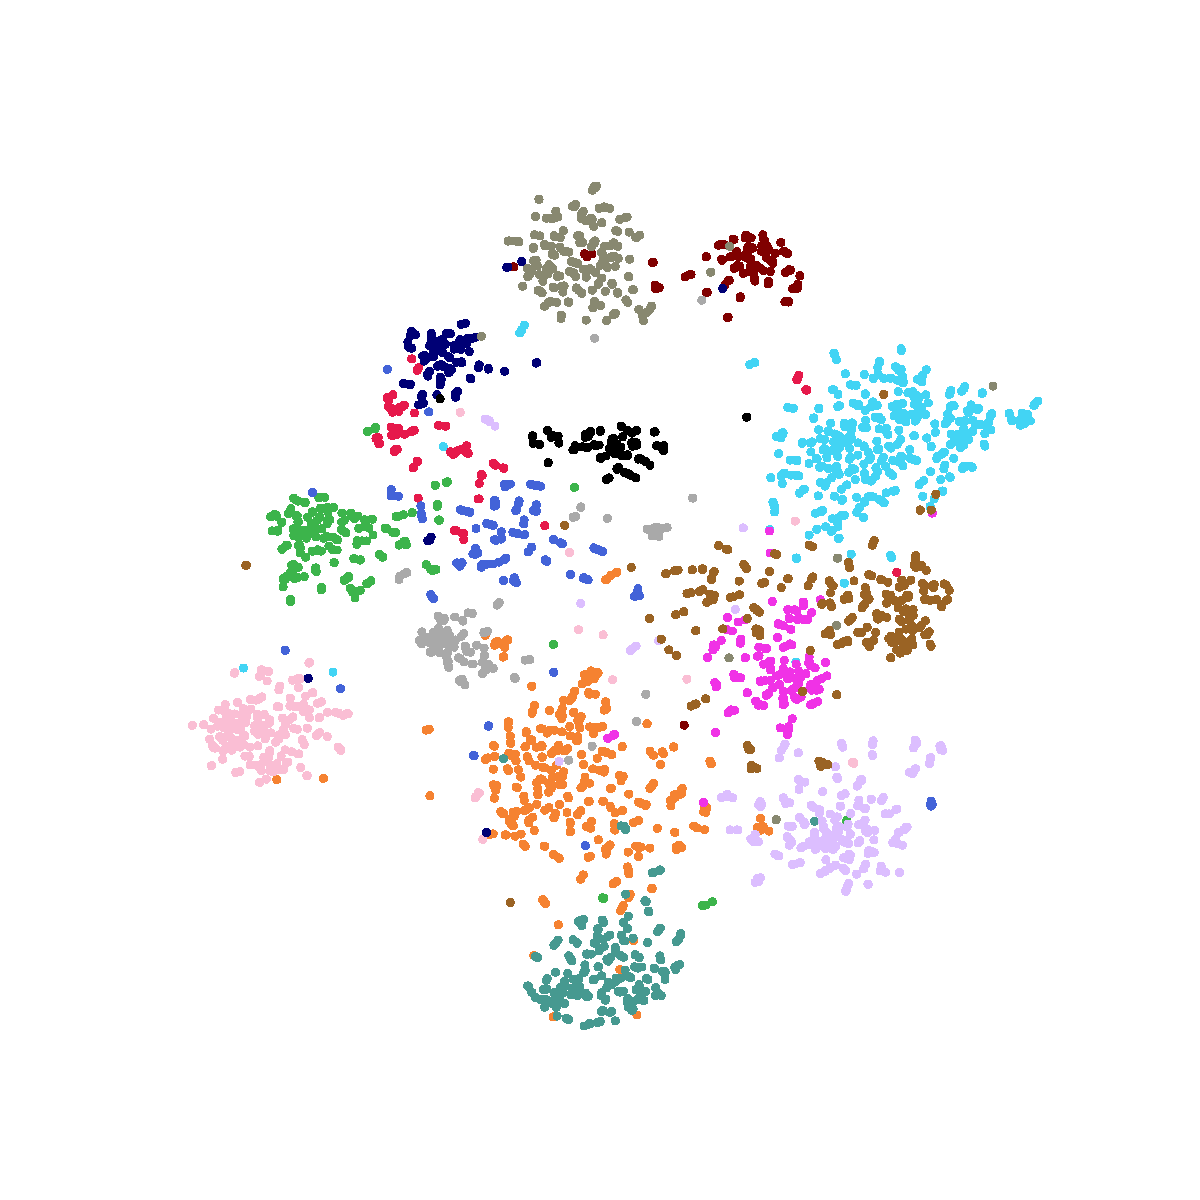
\includegraphics[width=\linewidth]{fig/tsne/point_mae.pdf}
        \caption*{\textbf{\#TP}:22.1M \textbf{\#OA}:85.18}
        \caption{Full fine-tuning}
        \label{fig:sub1}
    \end{subfigure}
    \hfill
    \begin{subfigure}{0.19\textwidth}
        \centering
        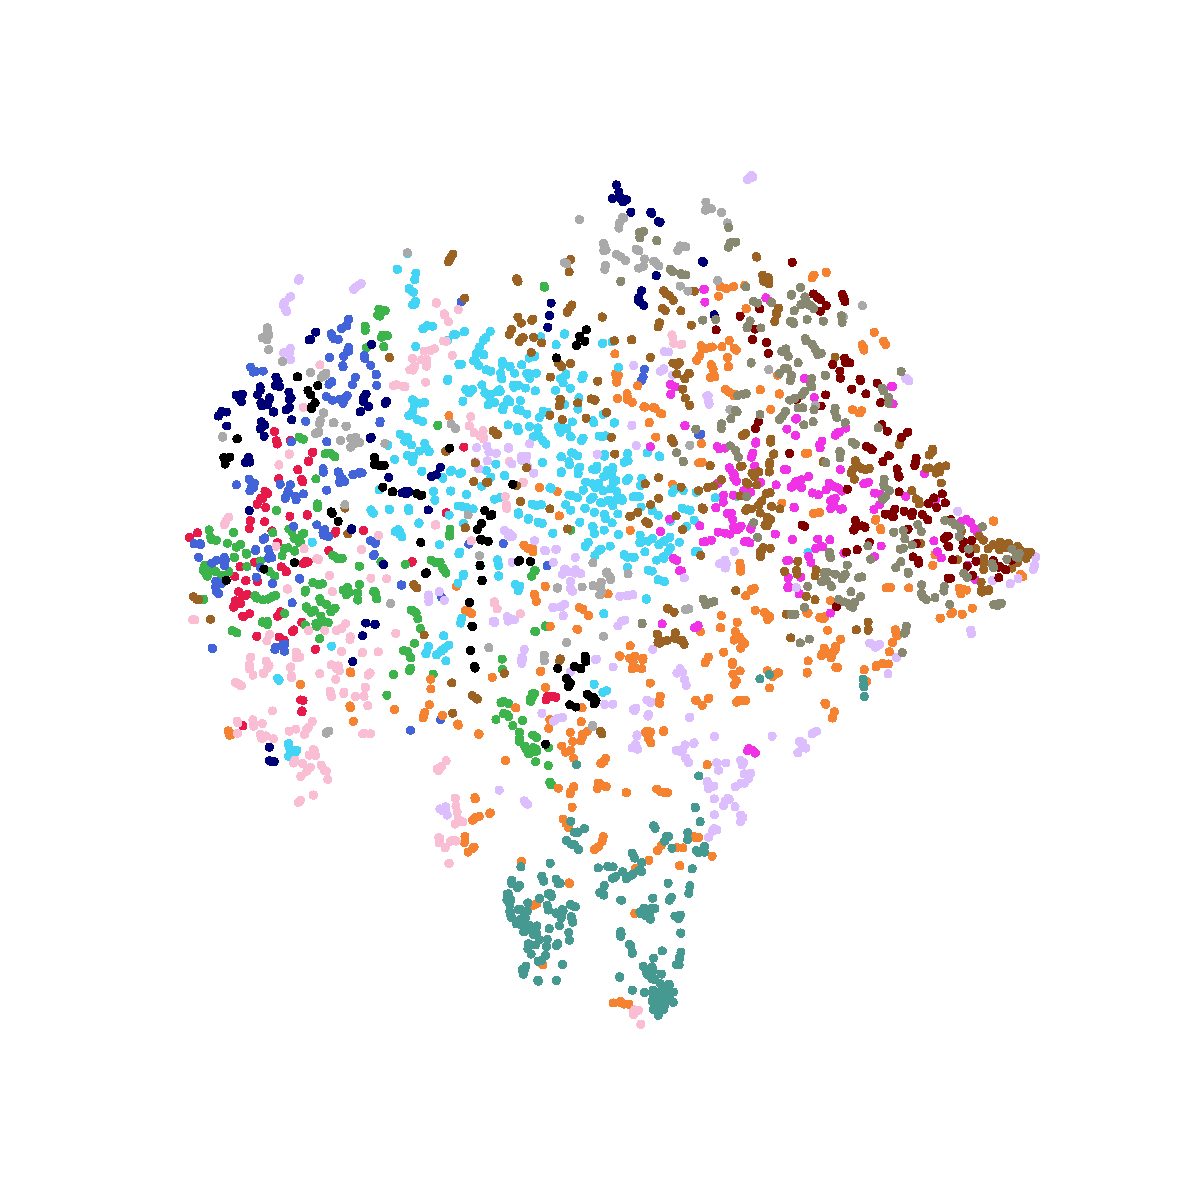
\includegraphics[width=\linewidth]{fig/tsne/LP.pdf}
        \caption*{\textbf{\#TP}:0.3M \textbf{\#OA}:75.99}
        \caption{Linear Probing}
        \label{fig:sub2}
    \end{subfigure}
    \hfill
    \begin{subfigure}{0.19\textwidth}
        \centering
        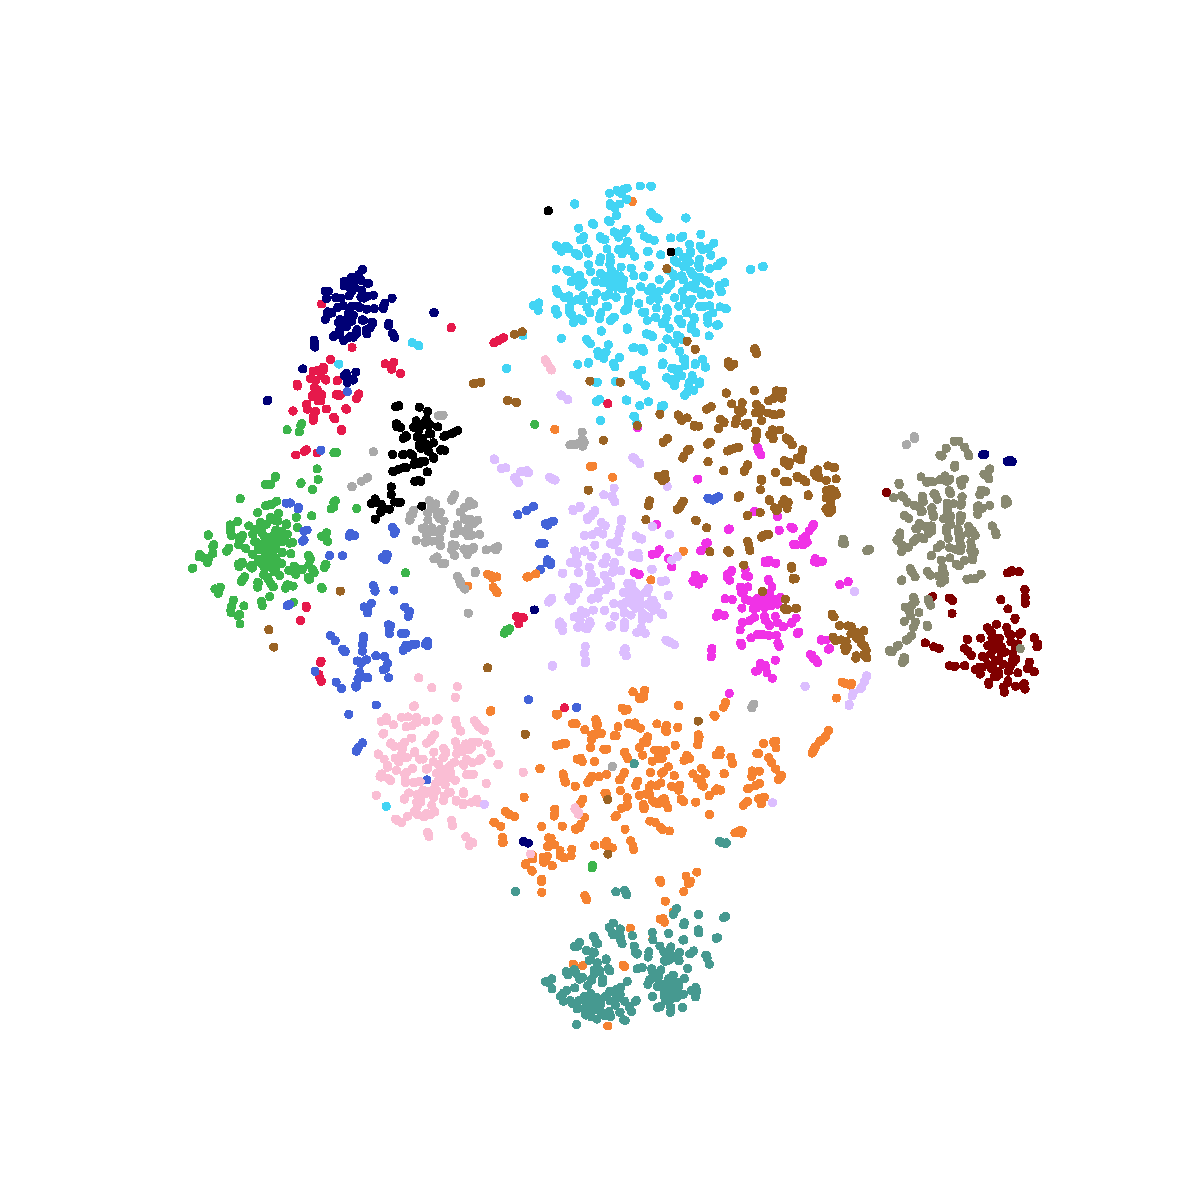
\includegraphics[width=\linewidth]{fig/tsne/idpt.pdf}
        \caption*{\textbf{\#TP}:1.7M \textbf{\#OA}:84.94}
        \caption{IDPT}
        \label{fig:sub3}
    \end{subfigure}
    \hfill
    \begin{subfigure}{0.19\textwidth}
        \centering
        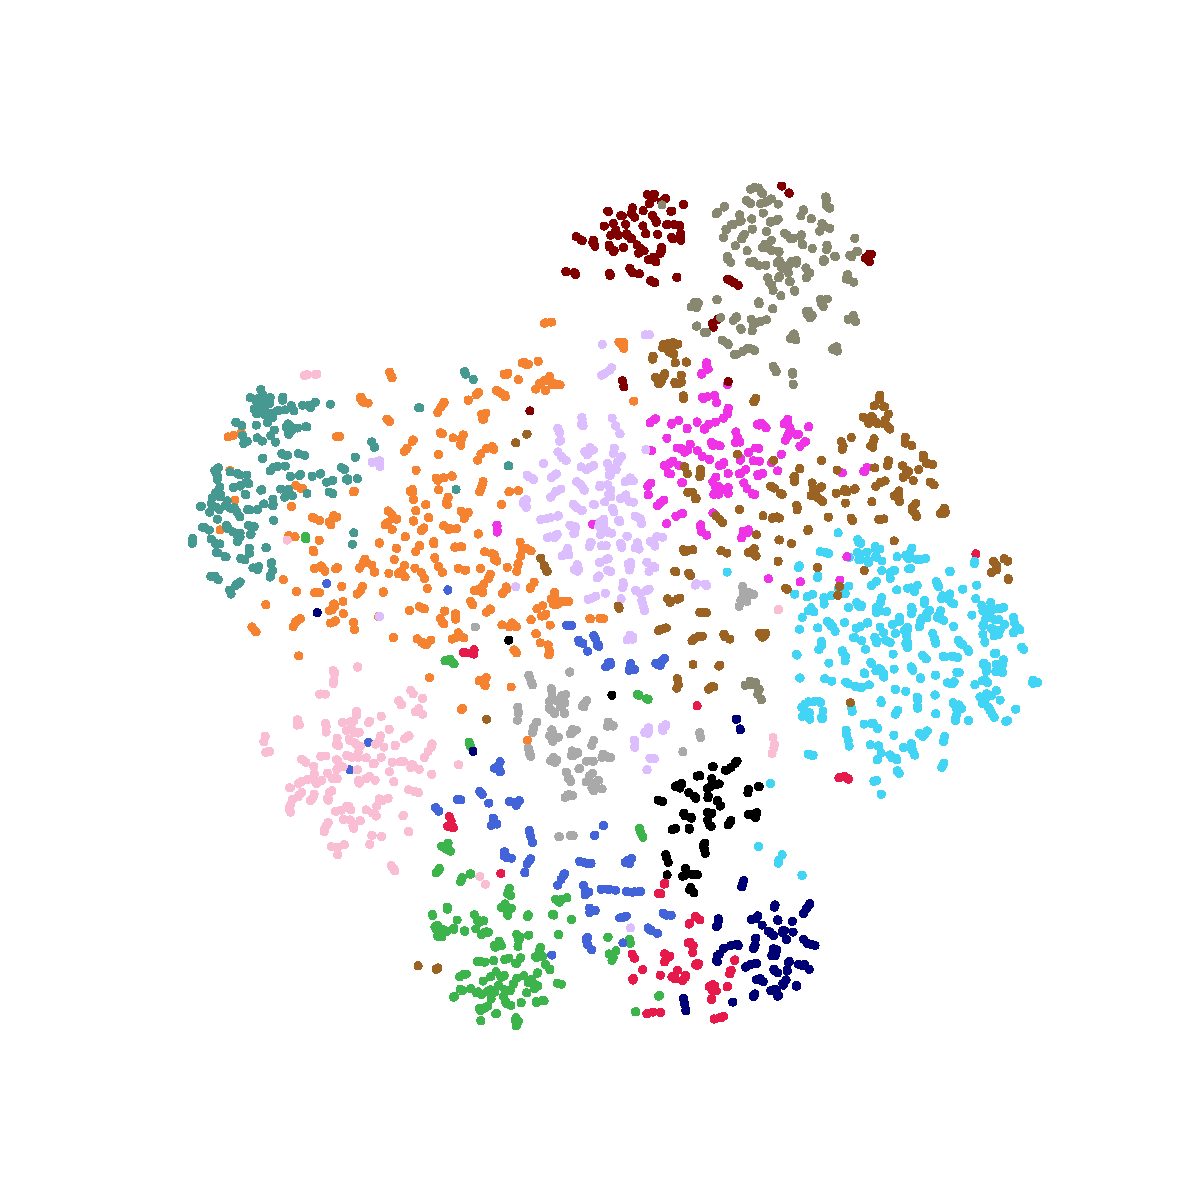
\includegraphics[width=\linewidth]{fig/tsne/dapt.pdf}
        \caption*{\textbf{\#TP}:1.1M \textbf{\#OA}:85.08}
        \caption{DAPT}
        \label{fig:sub4}
    \end{subfigure}
    % \hfill
    % \begin{subfigure}{0.24\textwidth}
    %     \centering
    %     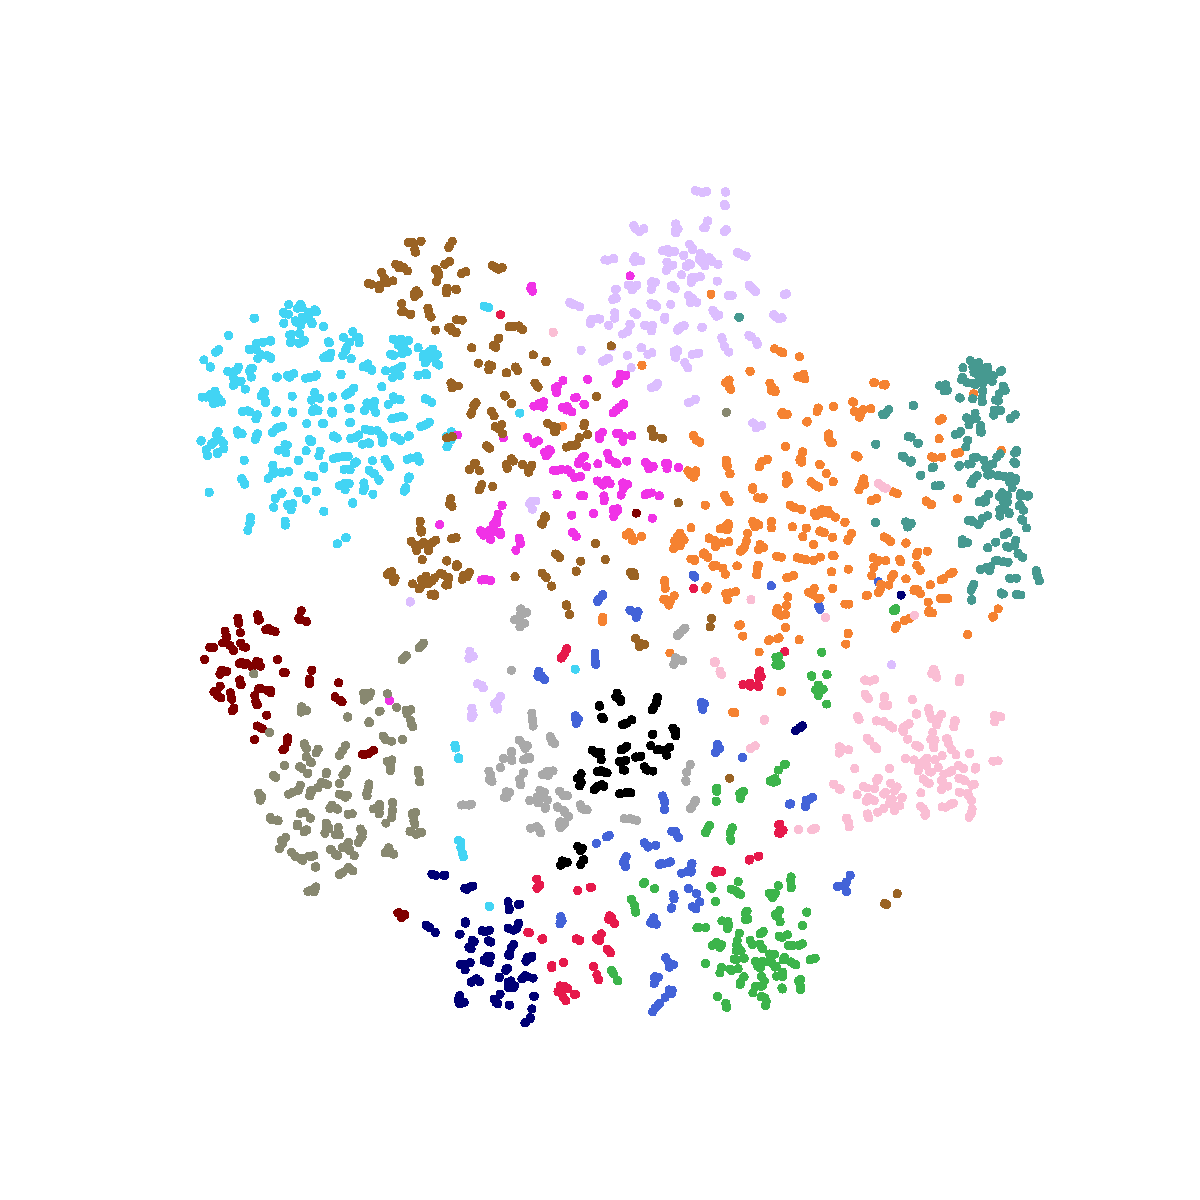
\includegraphics[width=\linewidth]{fig/tsne/pointgst.pdf}
    %     \caption*{\textbf{\#TP}:0.6M \textbf{\#OA}:85.29}
    %     \caption{PointGST}
    %     \label{fig:sub5}
    % \end{subfigure}
    % \hfill
    % \begin{subfigure}{0.24\textwidth}
    %     \centering
    %     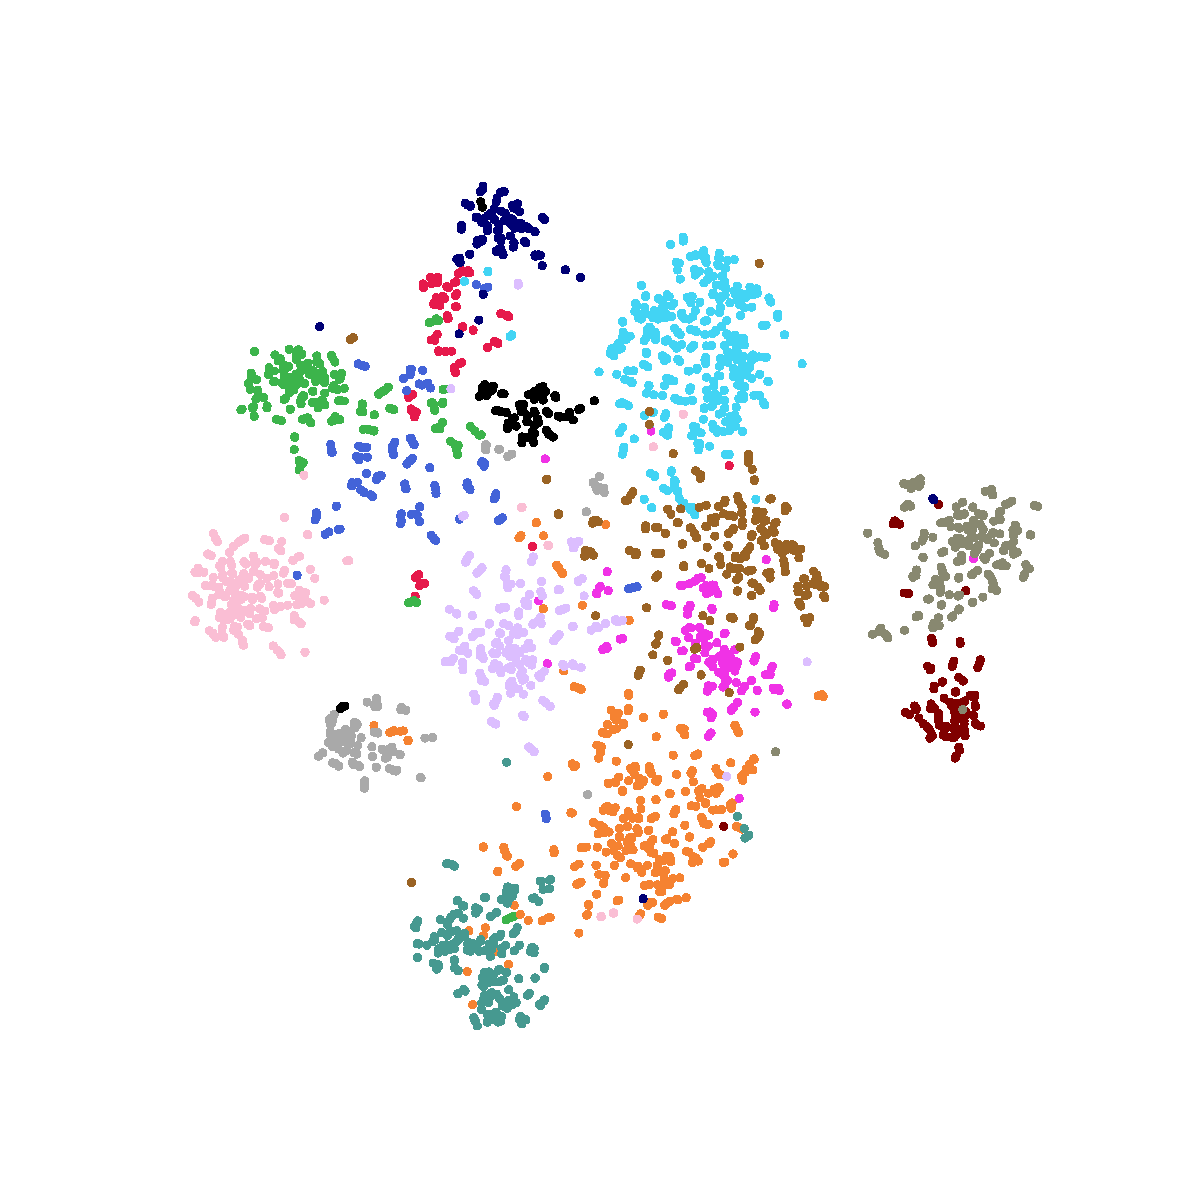
\includegraphics[width=\linewidth]{fig/tsne/PPT.pdf}
    %     \caption*{\textbf{\#TP}:1.1M \textbf{\#OA}:84.91}
    %     \caption{PPT}
    %     \label{fig:sub6}
    % \end{subfigure}
    % \hfill
    % \begin{subfigure}{0.24\textwidth}
    %     \centering
    %     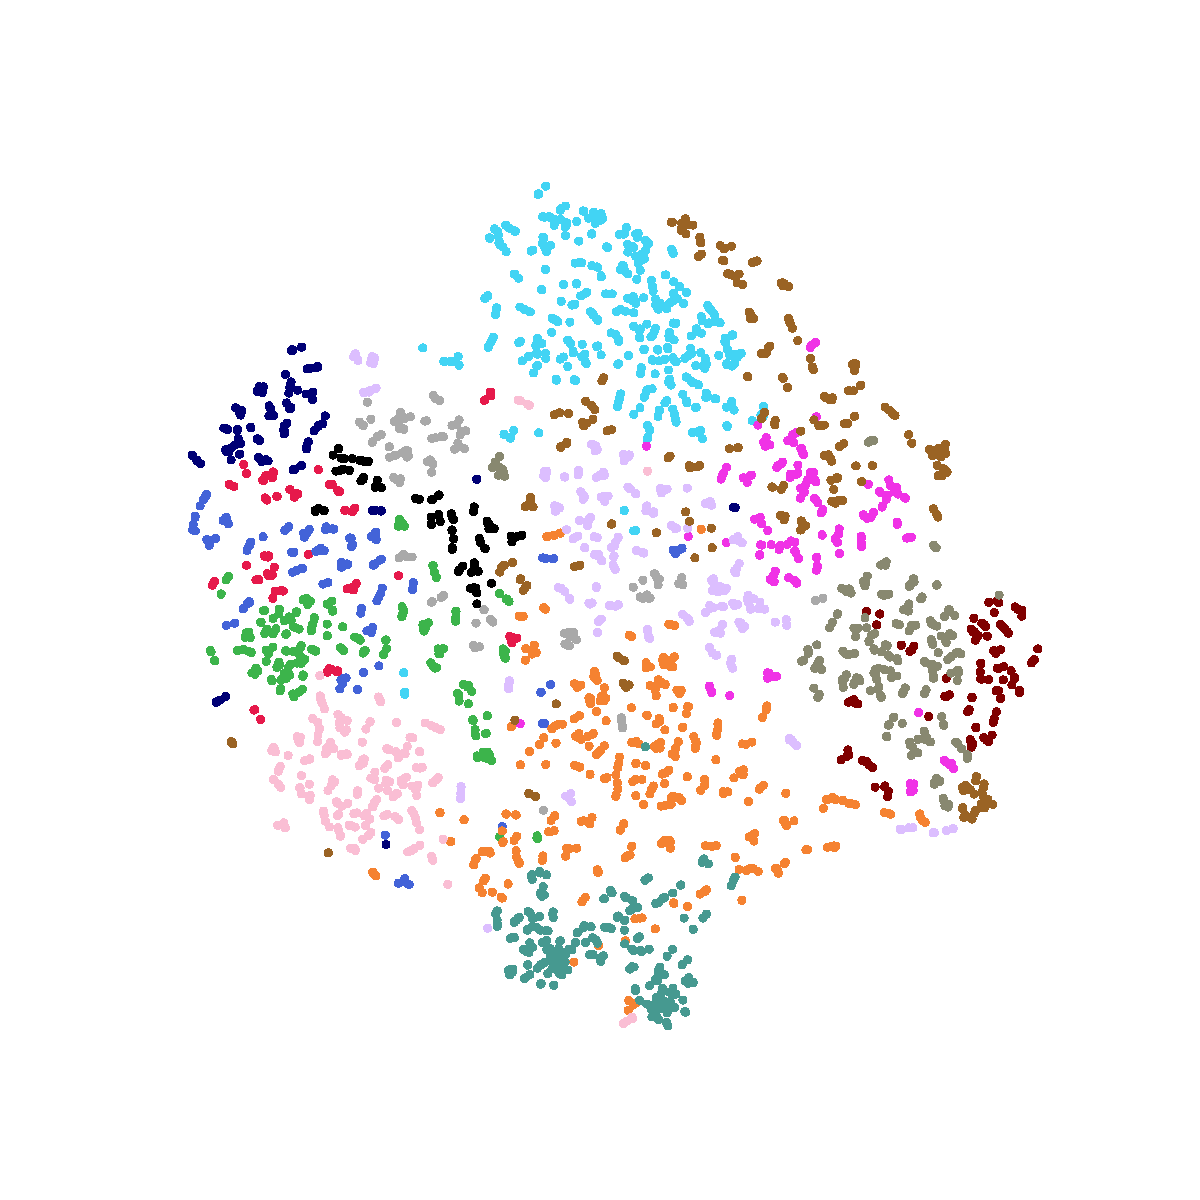
\includegraphics[width=\linewidth]{fig/tsne/LST.pdf}
    %     \caption*{\textbf{\#TP}:0.8M \textbf{\#OA}:82.75}
    %     \caption{LST}
    %     \label{fig:sub7}
    % \end{subfigure}
    \hfill
    \begin{subfigure}{0.19\textwidth}
        \centering
        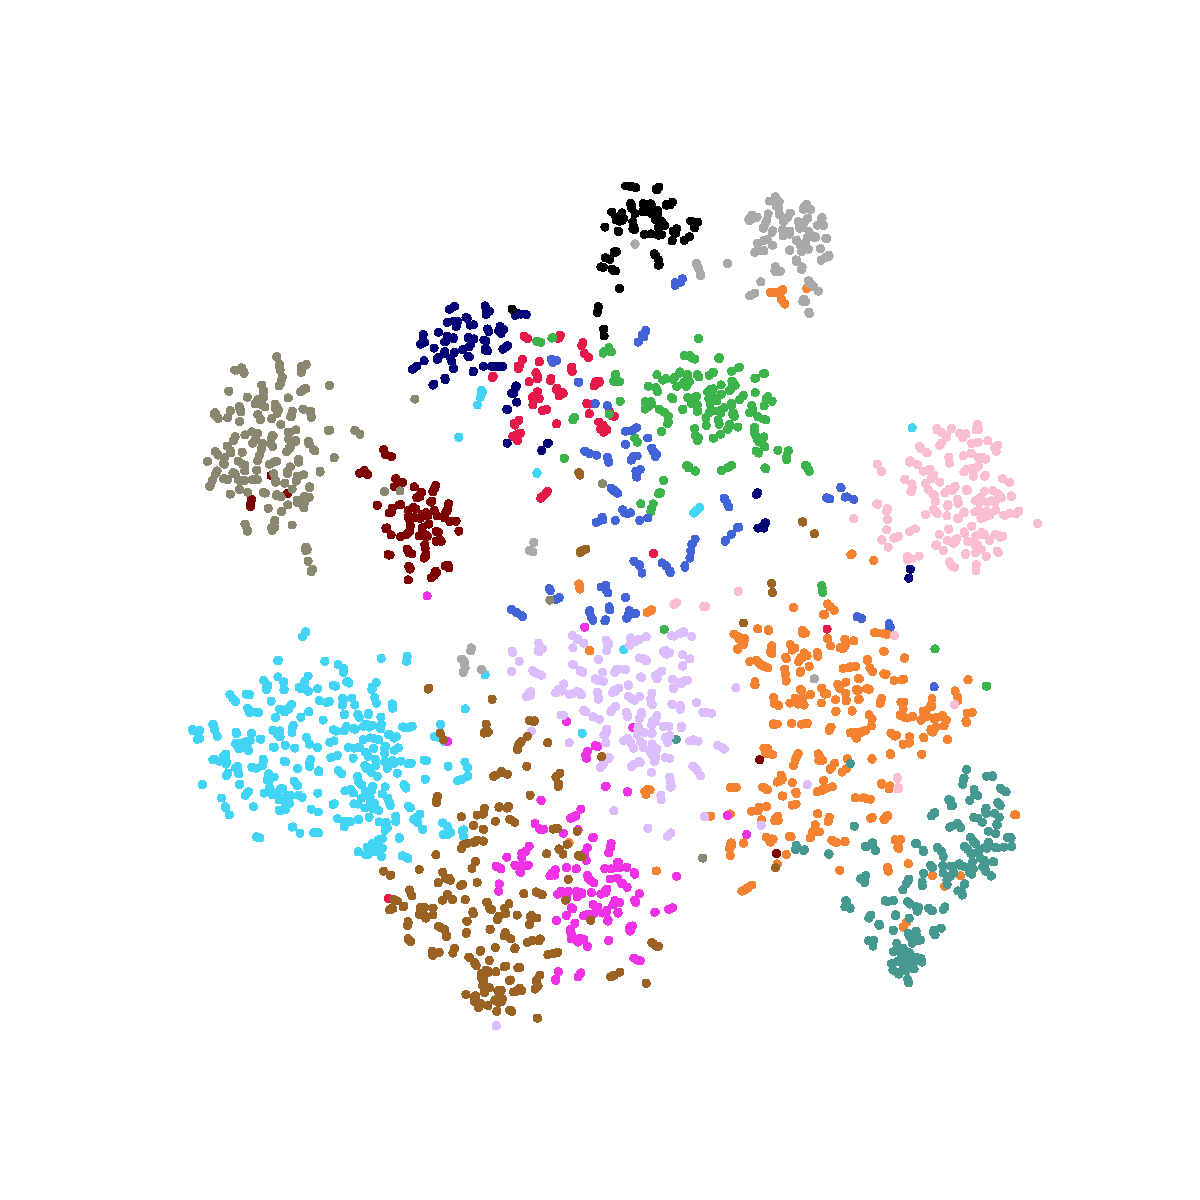
\includegraphics[width=\linewidth]{fig/tsne/point_ladder.pdf}
        \caption*{\textbf{\#TP}:0.6M \textbf{\#OA}:85.53}
        \caption{PLT (Ours)}
        \label{fig:sub8}
    \end{subfigure}
    \caption{The visualization of the t-SNE~\cite{van2008visualizing} from the test sets of ScanObjectNN~\cite{uy2019revisiting} (PB\_T50\_RS) by using a pre-trained PointMAE~\cite{pang2022masked} with various fine-tuning strategies. We extract the final classification features from the top linear layer for t-SNE visualizations.}
    \label{fig:tsne}
\end{figure*}

\subsection{Performance Analysis}

Tab.\ref{tab:performance} provides a comprehensive comparison of our PLT framework against various recent parameter-efficient tuning methods built upon the Point-MAE\cite{pang2022masked} baseline. The evaluation is conducted on the most challenging variant of ScanObjectNN~\cite{uy2019revisiting} (i.e., PB\_T50\_RS), with consistent settings including a batch size of 32 and all throughput metrics measured on a single NVIDIA RTX 3090 GPU.

Our method achieves the best accuracy (85.53\%) among all competing approaches, outperforming the original full fine-tuning baseline (85.18\%) and other prompt tuning or adapter-based methods. Notably, PLT accomplishes this with only 0.60M trainable parameters—merely 2.7\% of the full Point-MAE model—demonstrating remarkable parameter efficiency. In comparison, methods such as IDPT~\cite{zha2023instance} (1.70M) and DAPT~\cite{zhou2024dynamic} (1.09M) use significantly more parameters while yielding inferior accuracy.

In terms of computational complexity, PLT maintains a moderate FLOPs level (5.02GFLOPs), comparable to the baseline PointMAE~\cite{pang2022masked} (4.93GFLOPs) and much lower than IDPT~\cite{zha2023instance} (7.27GFLOPs), further validating its lightweight design. From a practical deployment standpoint, PLT achieves favorable training throughput (165.4 samples/s) and inference speed (210.8 samples/s), striking a solid balance between speed and effectiveness. While DAPT offers slightly higher training throughput (169.0 samples/s), its inference accuracy and parameter efficiency are not as competitive.

Memory usage is also a critical factor. PLT maintains low inference memory (0.85G), on par with most methods and substantially better than PointPEFT~\cite{tang2024point} (1.12G). Although the incorporation of FPS and KNN operations in PLT leads to a moderate increase in training memory consumption (2.26G), the overhead remains acceptable in practical applications. Notably, PLT still maintains a significantly lower memory footprint compared to other methods (e.g. PointPEFT~\cite{tang2024point} (8.64G) and IDPT~\cite{zha2023instance} (5.10G)) that also rely on similar operations.

Overall, PLT demonstrates strong performance across all dimensions—achieving top-tier accuracy with minimal parameters, competitive FLOPs, efficient inference and training speeds, and modest memory consumption. This highlights its suitability for real-world deployment where both effectiveness and efficiency are essential. Importantly, PLT achieves this without sacrificing the backbone architecture or requiring extensive architectural re-design, offering a plug-and-play solution compatible with powerful pretrained models like Point-MAE~\cite{pang2022masked}.
\section{Conclusion and Limitation}
\label{sec:conclusion&limitation}

In this paper, we introduced Point Ladder Tuning (PLT), a parameter-efficient fine-tuning strategy designed specifically for point cloud analysis. PLT freezes the parameters of the backbone network and employs a hierarchical Ladder Network (HLN) to extract local information directly from the input point cloud. To effectively integrate this local information with intermediate global features from the backbone network, we proposed a Local-Global Fusion (LGF) module. Furthermore, multi-scale fused features are leveraged to generate adaptive prompts, optimizing the backbone network's global features for downstream tasks. Our experiments demonstrate that PLT achieves competitive performance in tasks such as object classification and dense prediction, all while requiring minimal additional parameters. However, this study is limited to classification and segmentation tasks, leaving evaluations on other tasks, such as point cloud object detection and generation, as directions for future work.


{
    \small
    \bibliographystyle{ieeenat_fullname}
    \bibliography{main}
}

% WARNING: do not forget to delete the supplementary pages from your submission 
% \clearpage
\setcounter{page}{1}
\maketitlesupplementary
\appendix

\section{Dataset and Training Detail}

All experiments are conducted on a single GeForce RTX 3090 GPU. During training, we freeze the weights of the pre-trained model and only fine-tune a small number of parameters for adding modules. The hyperparameter settings of the model are shown in Tab.~\ref{tab:paramas}.

\textbf{ScanObjectNN}~\cite{uy2019revisiting} comprises approximately 15k point cloud samples across 15 categories captured in indoor scenes, often containing background interference and occlusions. There are three commonly-used variants, namely OBJ\_BG, OBJ\_ONLY, and PB\_T50\_RS, with the difficulty escalating successively. The training settings are in line with the baseline comparison. Specifically, the AdamW optimizer is employed with an initial learning rate of $5e^{-4}$ and a weight decay of 0.05. A cosine learning rate scheduler with 10 epochs of warm-up is also utilized. The model undergoes a total of 300 epochs of training, with a batch size of 32. For the sake of consistency, our sampling point cloud contains 2048 points, which are divided into 128 groups of 32 points each within the Patch Encoder.

\textbf{ModelNet}~\cite{wu20153d} contains 12,311 clean 3D CAD models spanning 40 categories. Under the full-sample training setting, the network training configuration aligns with that used for ScanObjectNN. In the few-shot experiments, the model is trained for a total of 150 epochs. The input point cloud consists of 1,024 points, which are divided into 64 groups in the Patch Encoder, with each group containing 32 points.

\textbf{ShapeNetPart}~\cite{yi2016scalable} is a widely used benchmark for point-level synthetic object part segmentation, comprising 16,881 samples across 16 object categories and 50 part categories. Training is conducted with the AdamW optimizer, employing a weight decay of $1e^{-4}$ and a cosine learning rate scheduler. The initial learning rate is set to $2e^{-4}$, with 11 epochs of warm-up. Models are trained for 300 epochs with a batch size of 16. Each input consists of 2,048 points, organized into 128 groups, with each group containing 32 points.

\textbf{S3DIS}~\cite{armeni20163d} is a large-scale indoor scene dataset encompassing six areas with a total of 273 million points across 13 categories. Consistent with prior studies~\cite{dong2022autoencoders}, we recommend using Area 5 for evaluation to ensure a more reliable and fair assessment of performance in semantic segmentation task. The model training employs a cosine learning rate scheduler, starting with an initial learning rate of $2e^{-4}$. Training is conducted over 60 epochs with a batch size of 32, while other configurations remain identical to those used for ShapeNetPart~\cite{yi2016scalable}.

\section{Additianal Experiments}

\subsection{Performance Analysis}
As illustrated in Fig.~\ref{fig:performance}, we compared the speed and memory usage of our PLT with previous methods during both training and inference. From Fig.~\ref{fig:per1}, we observe that with smaller batch sizes, our training speed is initially slower than that of full fine-tuning and even lower than IDPT. However, as the batch size increases, the training speed of our method surpasses that of full fine-tuning. Specifically, with a batch size of 128, our method is nearly 30\% faster than IDPT. Fig.~\ref{fig:per2} shows that our method consistently uses less training memory than full fine-tuning. In contrast, both IDPT and Point PEFT exhibit higher memory usage than full fine-tuning. Notably, with a batch size of 256, our approach reduces memory usage by 1.2 GB compared to full fine-tuning. As depicted in Fig.~\ref{fig:per3}, our method consistently outperforms IDPT and Point PEFT in inference speed, coming close to but slightly below that of full fine-tuning. Furthermore, as shown in Fig.~\ref{fig:per4}, the difference in memory usage during inference between our method and full fine-tuning is minimal. In comparison, IDPT and Point PEFT exhibit significantly higher memory usage differences, particularly at a batch size of 512.

\subsection{Token Selections for Head Inputs}
We analyzed the impact of different input tokens on downstream task heads, including the pooling of class token, prompt tokens, point patch tokens, and HLN output tokens. As illustrated in Figure 3, we evaluated five standard token selection methods. The results show that the best performance is achieved when all four token types are included. Interestingly, adding the pooled prompt tokens to the class token, rather than concatenating them, improves accuracy by 0.55\% while reducing the number of trainable parameters. Additionally, we observed that removing the point patch tokens leads to a more significant decline in performance compared to removing the prompt tokens or HLN output tokens. This highlights the critical role of prior information from pre-trained models in achieving high-quality downstream task performance.

\subsection{Qualitative Analysis}

\subsubsection{t-SNE Visualizations}
Fig.~\ref{fig:tsne} visualizes the t-SNE feature manifolds generated by fully fine-tuned methods, point-cloud-specific fine-tuning approaches such as IDPT and DAPT, and our proposed PLT, all trained on the ScanObjectNN PB\_T50\_RS dataset. The dispersion of points between categories in the t-SNE plot reflects the quality of the model's feature representation—greater inter-cluster dispersion and smaller intra-cluster average  distance  indicates stronger discriminative power, making classification tasks easier.

Notably, our PLT exhibits significantly greater inter-cluster dispersion alongside a smaller intra-cluster average  distance compared to previous methods. This suggests that our method effectively enhances the separation of features between categories while maintaining compactness within each category. Such properties indicate a superior ability to learn and represent discriminative features.

Moreover, PLT achieves these results while utilizing fewer learnable parameters, demonstrating its efficiency in leveraging pre-trained models to adapt to downstream tasks. This advantage not only reduces the computational cost but also highlights PLT’s potential for broader applicability in resource-constrained scenarios. Compared to fully fine-tuned and point cloud-specific methods, PLT strikes a better balance between parameter efficiency and representation quality, establishing its value in point-cloud-based learning tasks.

\subsubsection{Part Segmentation Visualizations}

In Fig.~\ref{fig:part_segmentation}, we present a visual demonstration of the partial segmentation outcomes achieved by our proposed PLT, which is based on the PointMAE baseline. Specifically, we choose five representative samples from different categories. For each of these selected samples, we render three distinct perspectives. It is evident from the figure that our method demonstrates remarkable segmentation performance. Notably, our PLT method achieves high accuracy and precisely distinguishes object parts while maintaining efficiency with a minimal parameter set.

\subsubsection{Semantic Segmentation Visualizations}

Fig.~\ref{fig:semantic} presents a qualitative comparison of segmentation results between our proposed PLT method and previous fine-tuning approaches on semantic segmentation tasks in Area 5 of the S3DIS dataset. The comparison highlights the strengths of PLT in addressing common challenges associated with point cloud segmentation. From the first row of the figure, it is evident that full fine-tuning, despite being resource-intensive, struggles with accurately segmenting object boundaries. This limitation often leads to poor boundary delineation and misclassification in continuous regions, largely due to inadequate capture of point cloud local information. A more detailed comparison in office\_9 demonstrates that methods such as full fine-tuning, IDPT, and DAPT misclassify walls as beams and clutter areas as ceilings. In contrast, our PLT approach successfully addresses these issues, accurately segmenting clutter regions while significantly reducing wall misclassification. Similarly, in office\_35, PLT outperforms other methods in segmenting challenging areas such as the clutter region and the board. Where methods like full fine-tuning, IDPT, and PPT struggle to recognize or segment these regions effectively, PLT demonstrates superior performance, maintaining clarity and precision. These results underscore the capability of our PLT method to achieve outstanding segmentation performance while using significantly fewer fine-tuning parameters. Compared to other approaches, PLT not only produces clearer segmentation boundaries but also exhibits a marked reduction in misclassifications, confirming its efficiency and effectiveness for point cloud semantic segmentation tasks.

\begin{table*}
\footnotesize
\setlength{\tabcolsep}{3.3mm}
\captionof{table}{Training details for downstream fine-tuning.}
% \vspace{-5pt}
\begin{tabular}{lcccccc}
\toprule
    \multirow{2}{*}{Configuration}  &\multicolumn{3}{c}{Classification} & \multicolumn{2}{c}{Segmentation}\\
		\cmidrule(r){2-4} \cmidrule(r){5-6}
	 &ScanObjectNN & ModelNet & ModelNet Few-shot & ShapeNetPart & S3DIS     \\
    \midrule
 Optimizer & AdamW & AdamW & AdamW & AdamW & AdamW \\
 Learning rate & $5 \times 10^{-4}$ & $5 \times 10^{-4}$ & $5 \times 10^{-4}$  & $2 \times 10^{-4}$ & $2 \times 10^{-4}$ \\
 Weight decay & $5 \times 10^{-2}$ & $5 \times 10^{-2}$ & $5 \times 10^{-2}$ & $5 \times 10^{-2}$  & $5 \times 10^{-2}$ \\
 Learning rate scheduler & cosine & cosine & cosine & cosine & cosine \\
 Training epochs  & 300 & 300 & 150 & 300 & 60 \\
 Warmup epochs& 10 & 10& 10 & 10 &10 \\
 Batch size & 32 & 32& 32 & 16 & 32 \\
 \midrule
 Number of points  & 2048 & 1024& 1024 & 2048 & 2048 \\
 Number of point patches & 128 & 64 & 64 & 128 & 128\\
 Point patch size  & 32 & 32 & 32  & 32 & 32 \\
 \midrule
 number of layers & 3 & 3 & 3 & 3 & 3\\
 HLN dims & [16, 32, 64, 128] & [16, 32, 64, 128] & [16, 32, 64, 128] & [32, 64, 128, 256] & [32, 64, 128, 256]\\
 HLN strides & [4, 4, 4] & [4, 4, 4] & [4, 4, 4] & [4, 2, 2] & [4, 2, 2]\\
 number of neighbors in HLN & [16, 8, 4] & [16, 8, 4] & [16, 8, 4] & [32, 16, 8] & [32, 16, 8] \\
\bottomrule
% \vspace{10pt}
\end{tabular}
\label{tab:paramas}
\end{table*}

\begin{figure*}
    \centering
    \begin{subfigure}{0.19\textwidth}
        \centering
        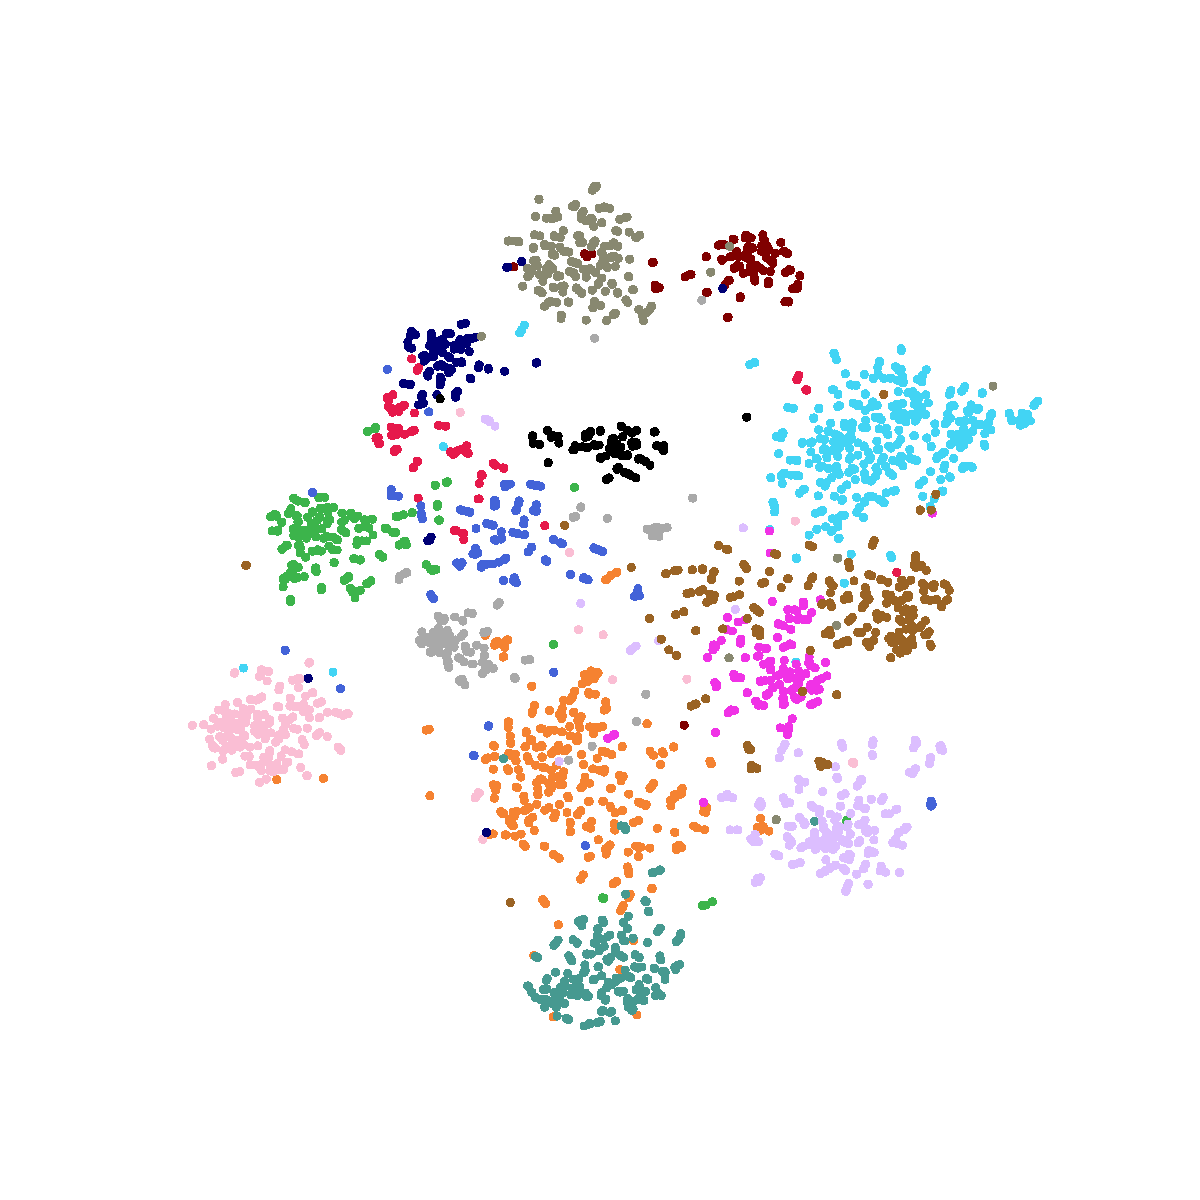
\includegraphics[width=\linewidth]{fig/tsne/point_mae.pdf}
        \caption*{\textbf{\#TP}:22.1M \textbf{\#OA}:85.18}
        \caption{Full fine-tuning}
        \label{fig:sub1}
    \end{subfigure}
    \hfill
    \begin{subfigure}{0.19\textwidth}
        \centering
        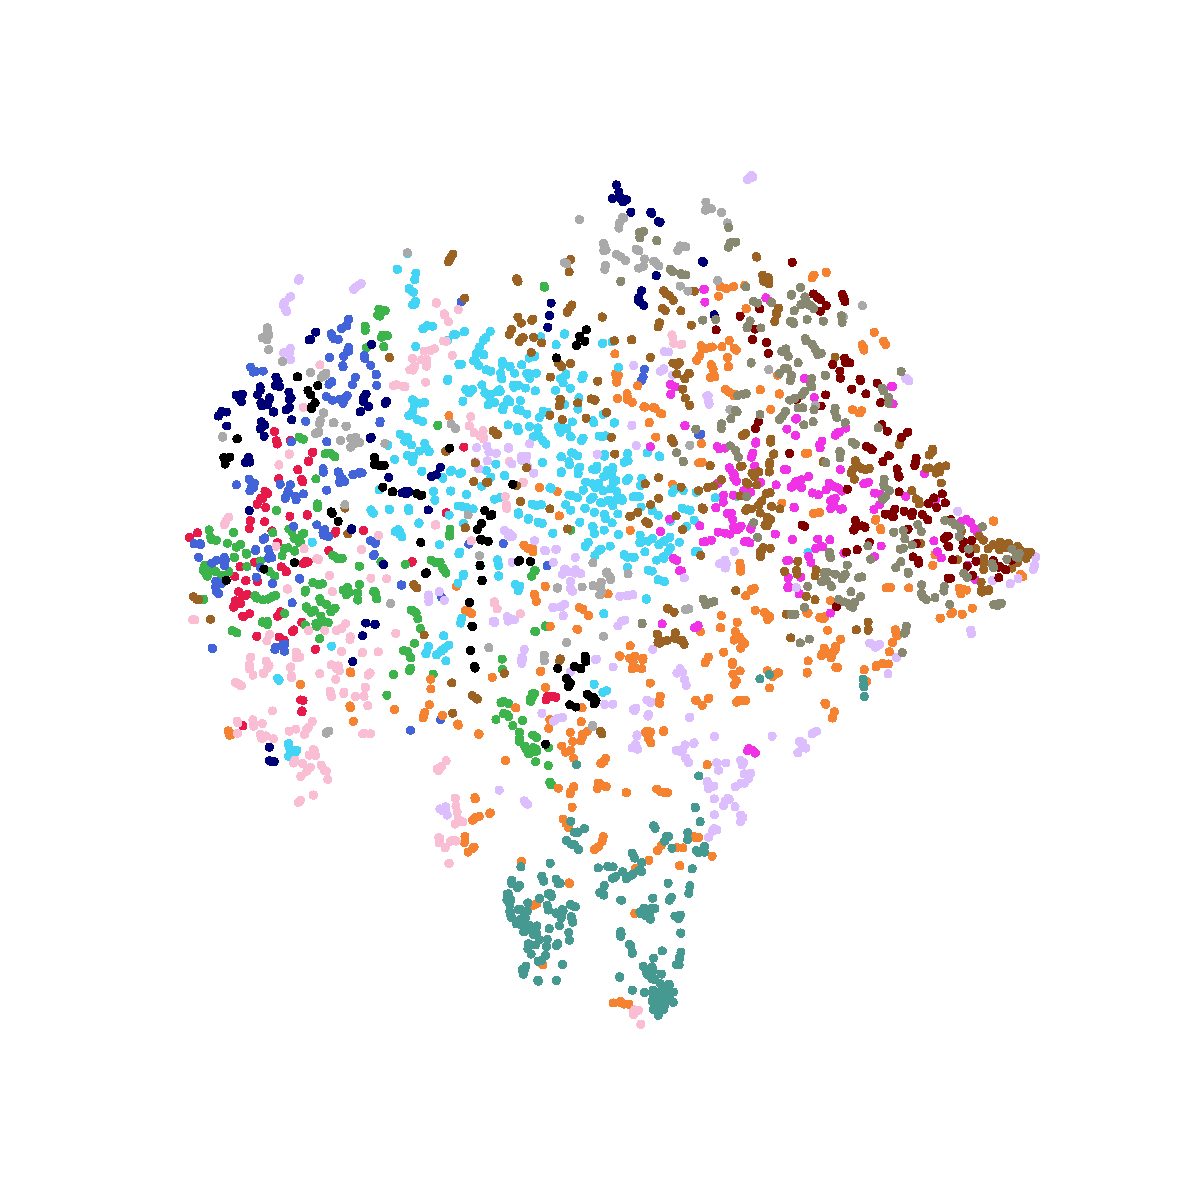
\includegraphics[width=\linewidth]{fig/tsne/LP.pdf}
        \caption*{\textbf{\#TP}:0.3M \textbf{\#OA}:75.99}
        \caption{Linear Probing}
        \label{fig:sub2}
    \end{subfigure}
    \hfill
    \begin{subfigure}{0.19\textwidth}
        \centering
        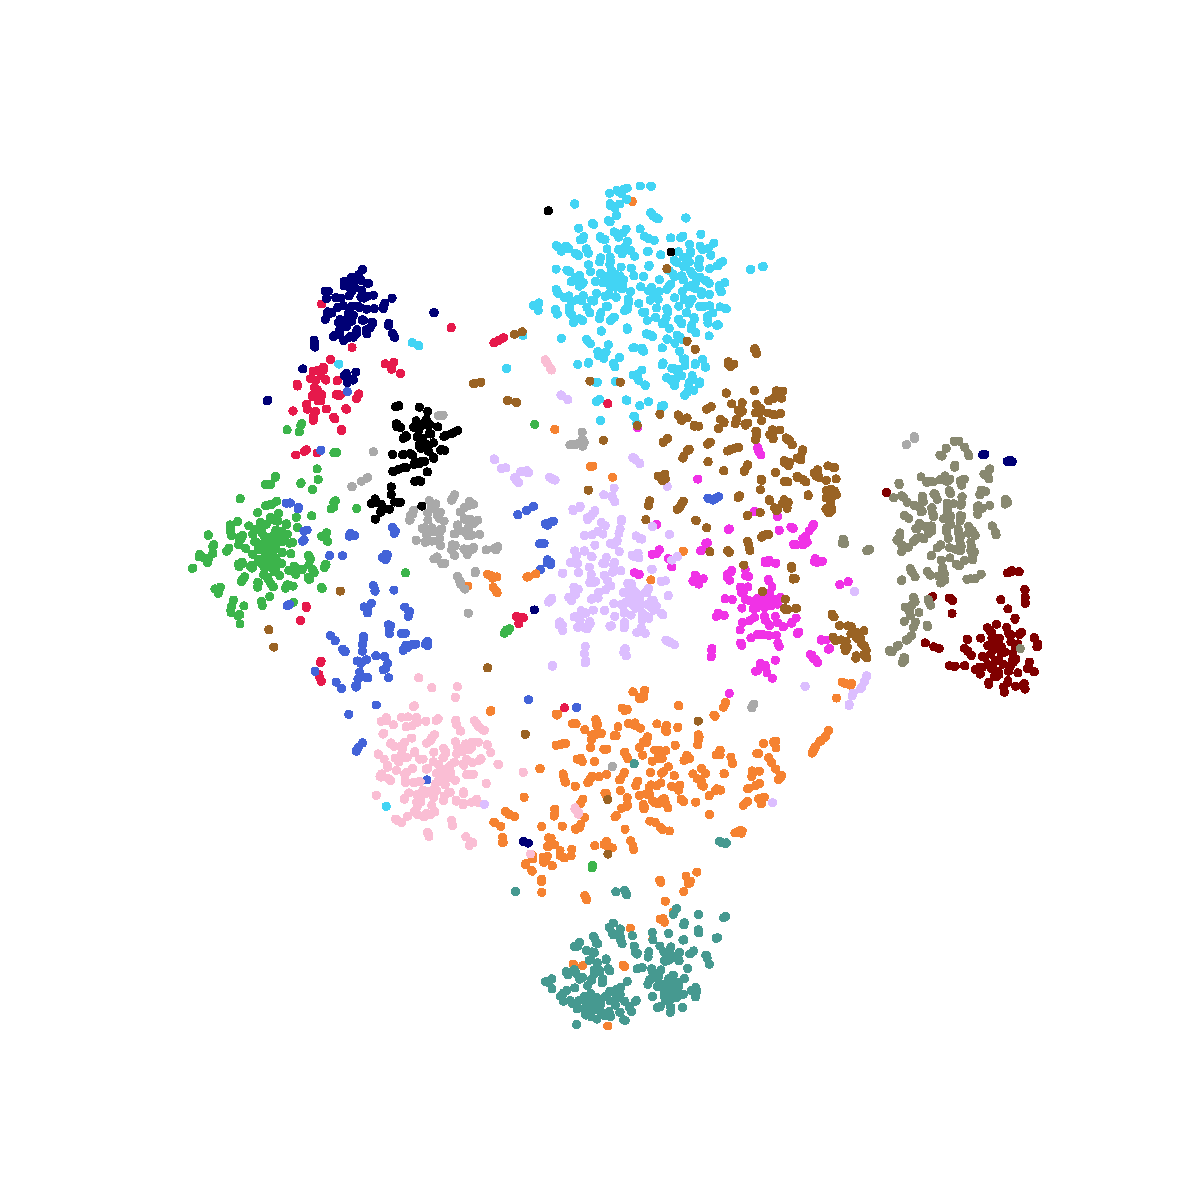
\includegraphics[width=\linewidth]{fig/tsne/idpt.pdf}
        \caption*{\textbf{\#TP}:1.7M \textbf{\#OA}:84.94}
        \caption{IDPT}
        \label{fig:sub3}
    \end{subfigure}
    \hfill
    \begin{subfigure}{0.19\textwidth}
        \centering
        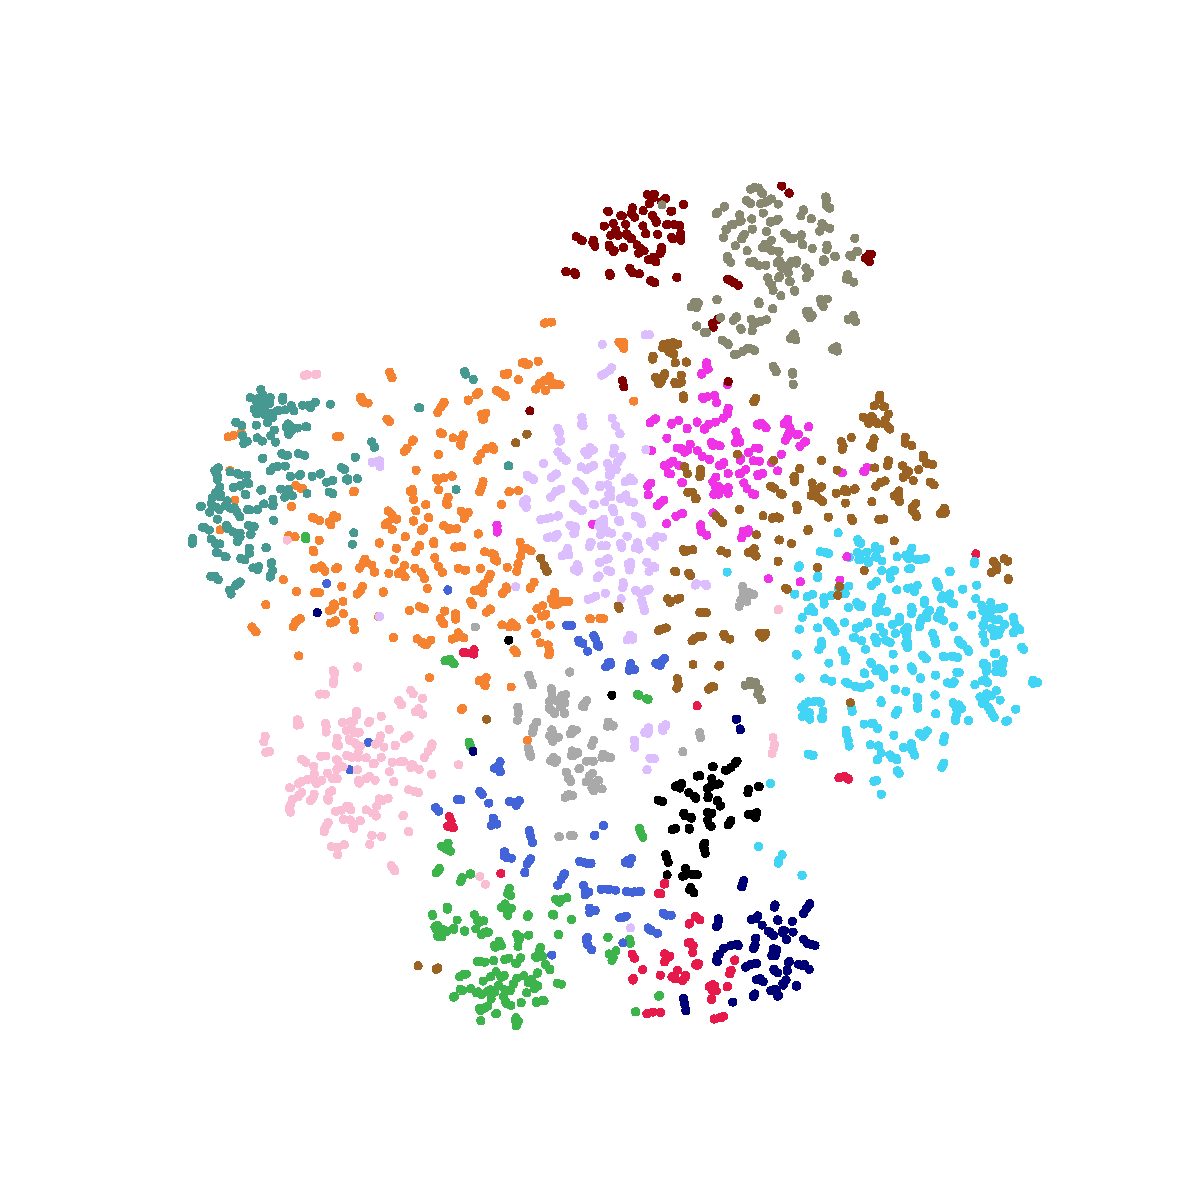
\includegraphics[width=\linewidth]{fig/tsne/dapt.pdf}
        \caption*{\textbf{\#TP}:1.1M \textbf{\#OA}:85.08}
        \caption{DAPT}
        \label{fig:sub4}
    \end{subfigure}
    % \hfill
    % \begin{subfigure}{0.24\textwidth}
    %     \centering
    %     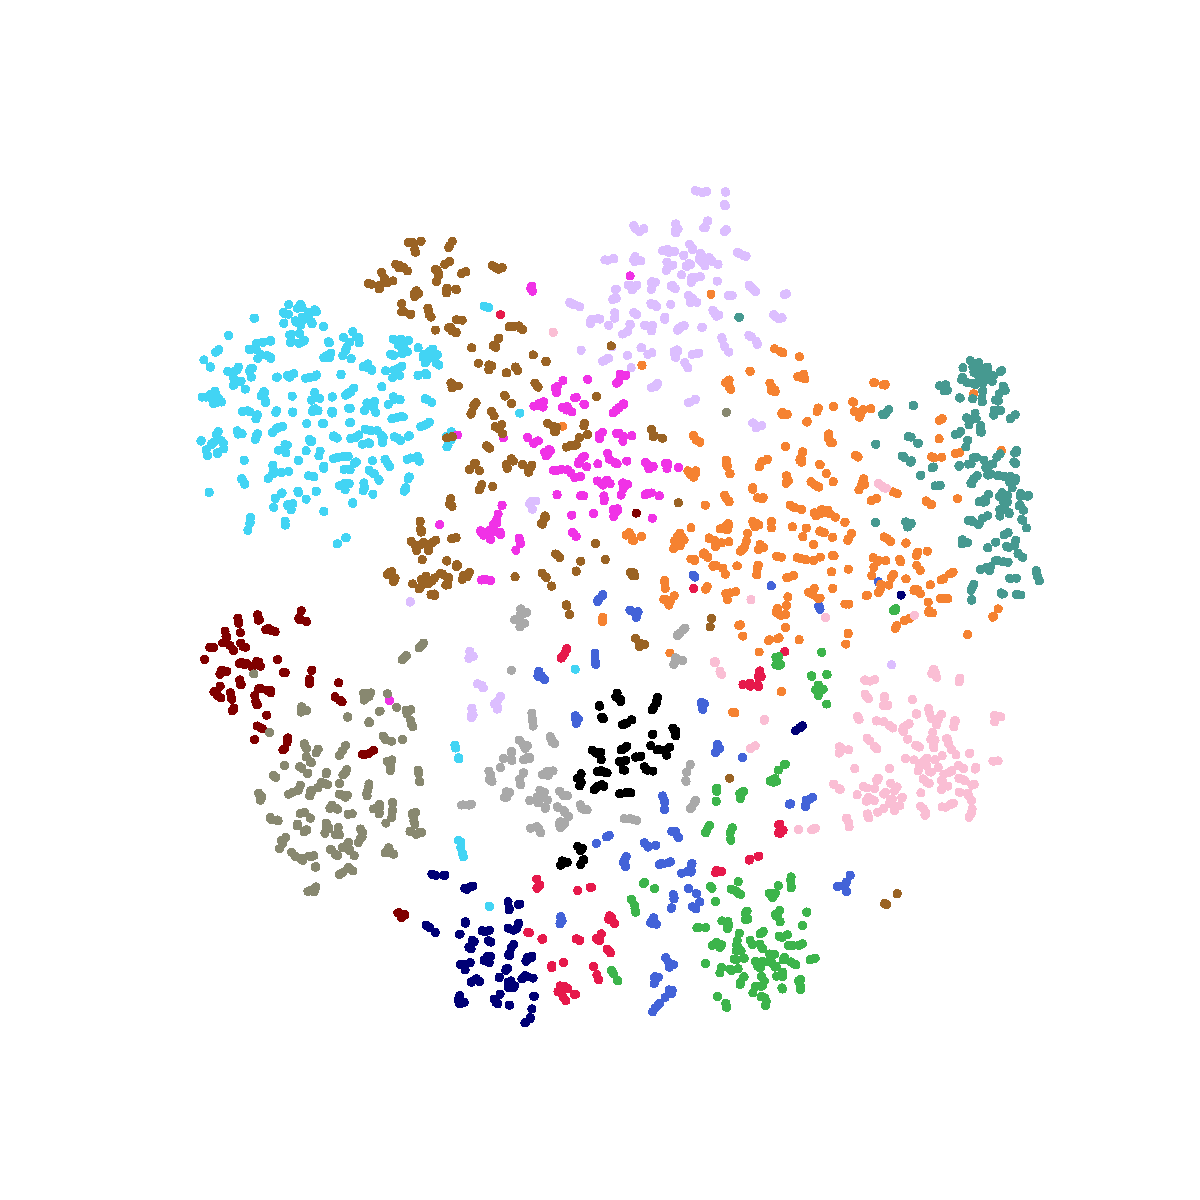
\includegraphics[width=\linewidth]{fig/tsne/pointgst.pdf}
    %     \caption*{\textbf{\#TP}:0.6M \textbf{\#OA}:85.29}
    %     \caption{PointGST}
    %     \label{fig:sub5}
    % \end{subfigure}
    % \hfill
    % \begin{subfigure}{0.24\textwidth}
    %     \centering
    %     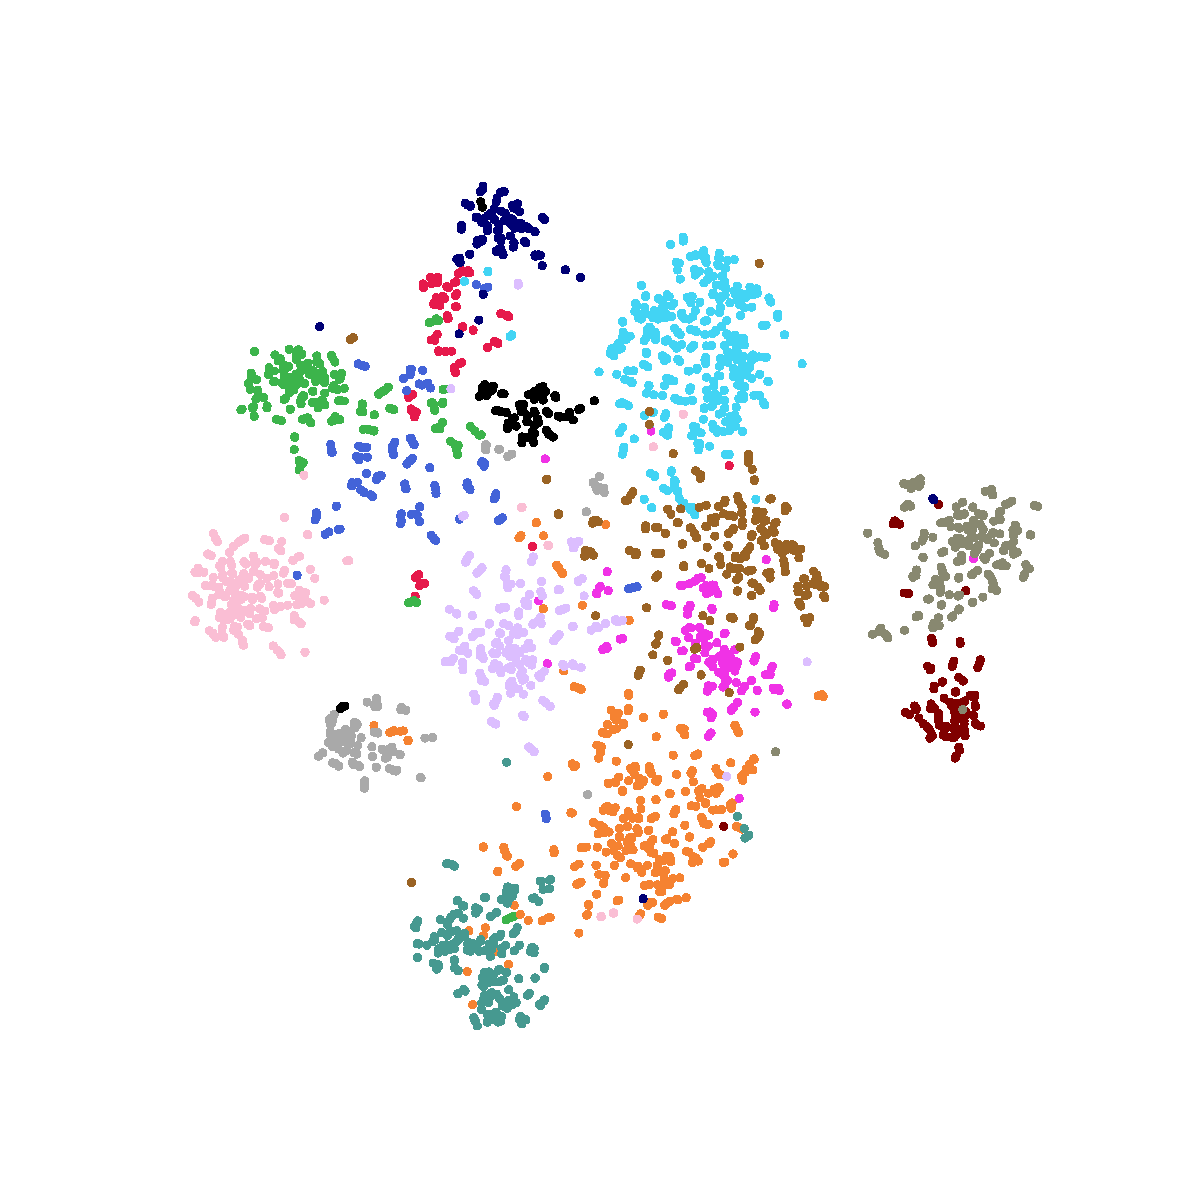
\includegraphics[width=\linewidth]{fig/tsne/PPT.pdf}
    %     \caption*{\textbf{\#TP}:1.1M \textbf{\#OA}:84.91}
    %     \caption{PPT}
    %     \label{fig:sub6}
    % \end{subfigure}
    % \hfill
    % \begin{subfigure}{0.24\textwidth}
    %     \centering
    %     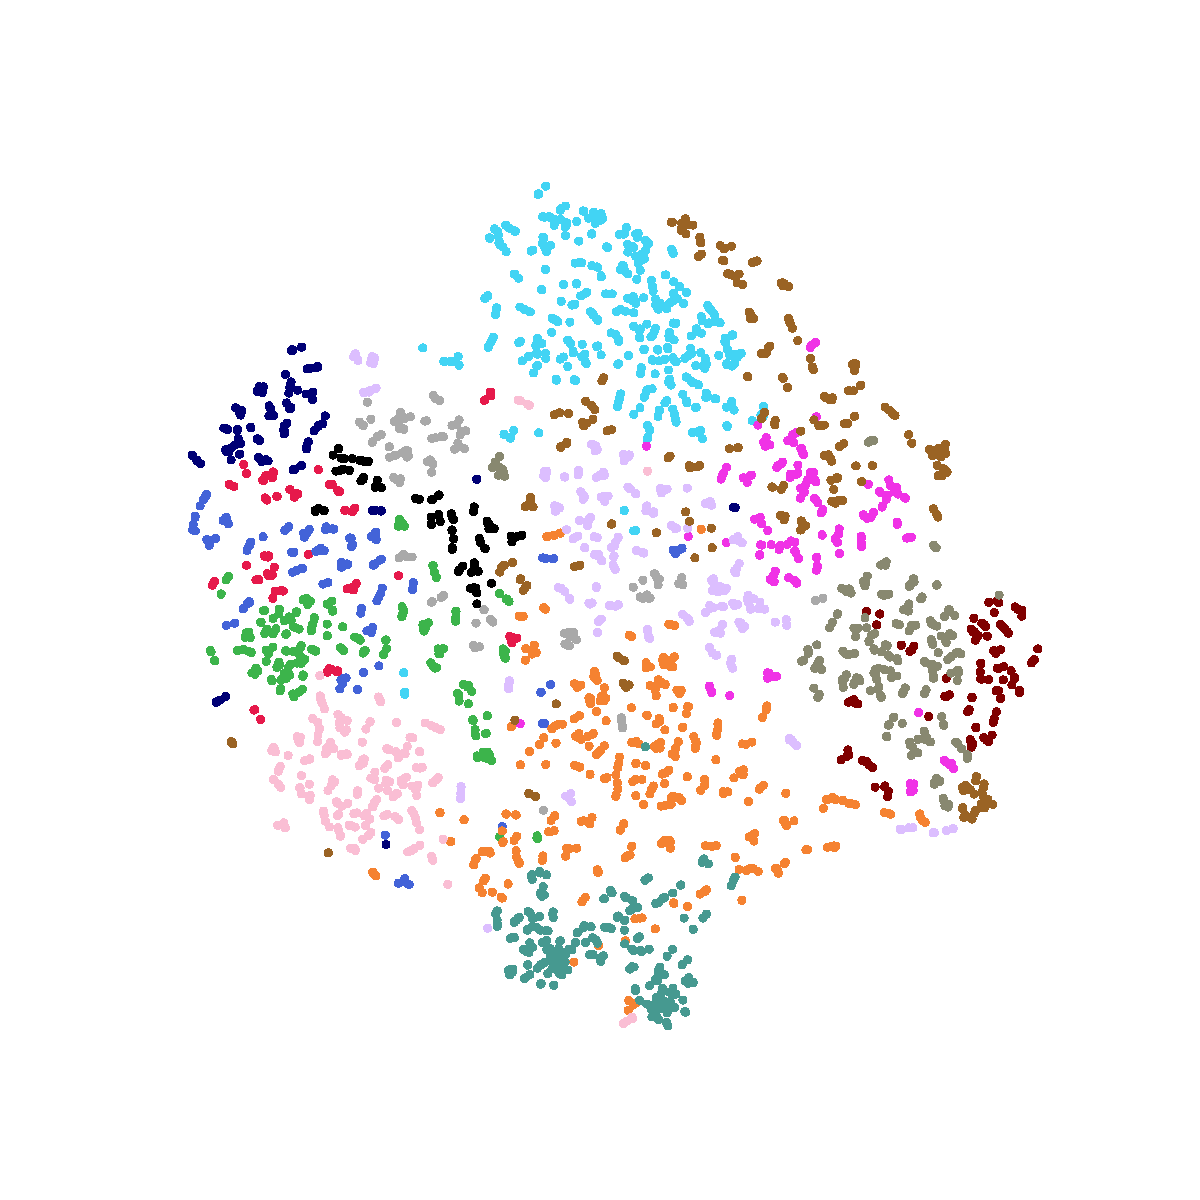
\includegraphics[width=\linewidth]{fig/tsne/LST.pdf}
    %     \caption*{\textbf{\#TP}:0.8M \textbf{\#OA}:82.75}
    %     \caption{LST}
    %     \label{fig:sub7}
    % \end{subfigure}
    \hfill
    \begin{subfigure}{0.19\textwidth}
        \centering
        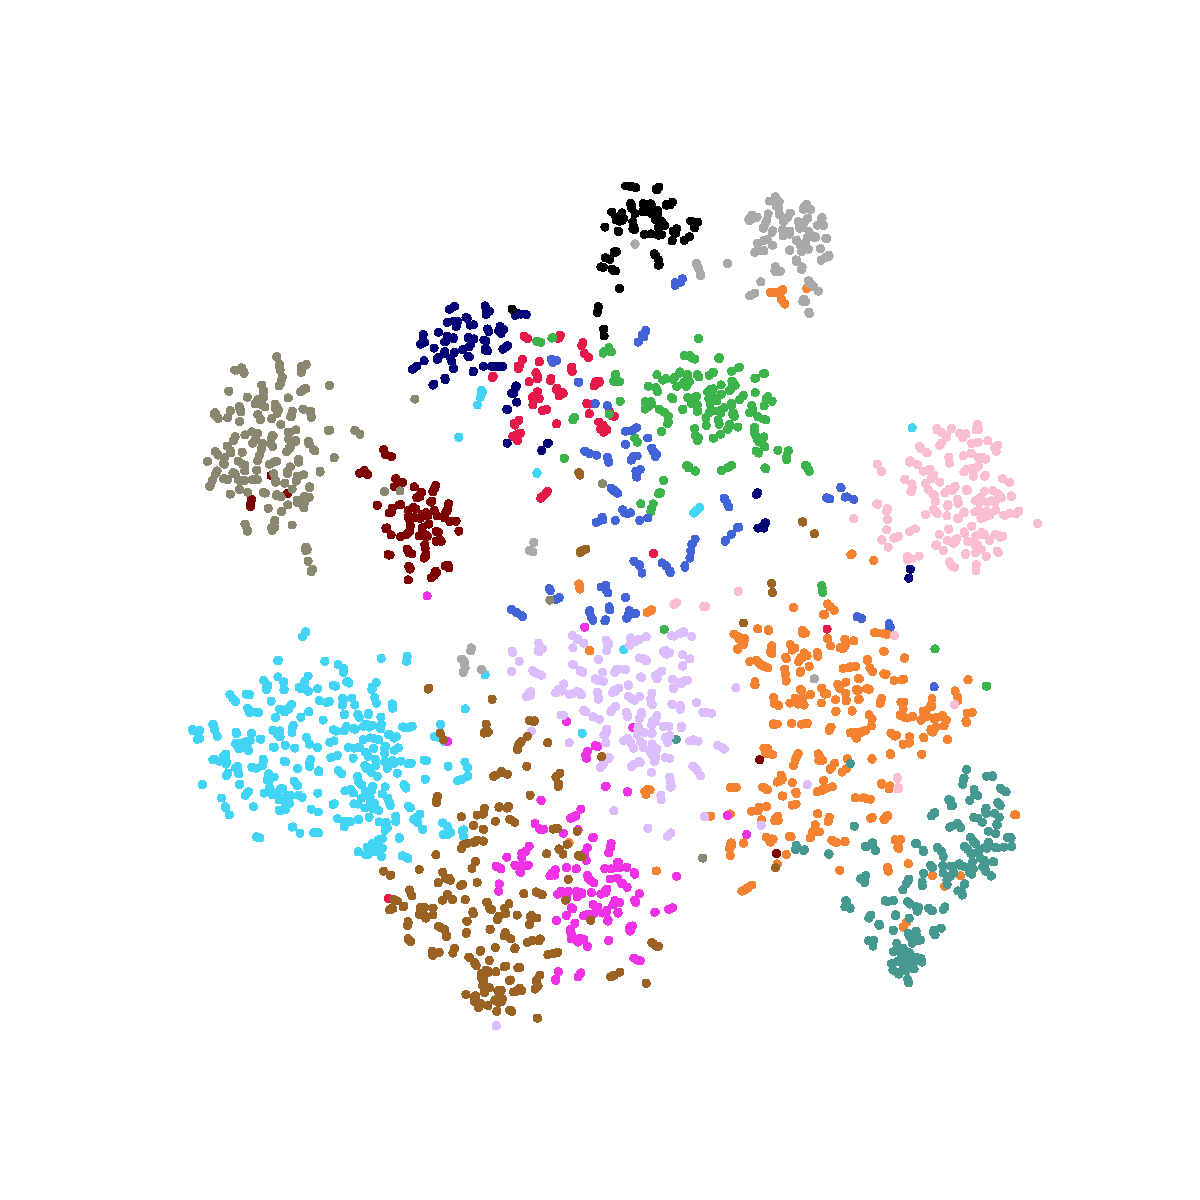
\includegraphics[width=\linewidth]{fig/tsne/point_ladder.pdf}
        \caption*{\textbf{\#TP}:0.6M \textbf{\#OA}:85.53}
        \caption{PLT (Ours)}
        \label{fig:sub8}
    \end{subfigure}
    \caption{The visualization of the t-SNE~\cite{van2008visualizing} from the test sets of ScanObjectNN~\cite{uy2019revisiting} (PB\_T50\_RS) by using a pre-trained PointMAE~\cite{pang2022masked} with various fine-tuning strategies. We extract the final classification features from the top linear layer for t-SNE visualizations.}
    \label{fig:tsne}
\end{figure*}

\begin{figure*}
    \centering
    \includegraphics[width=\linewidth]{fig/Effect of different inputs for downstream task head.pdf}
    \caption{Effect of different inputs for downstream classification task head. We conduct experiments on the hardest variant (i.e., PB\_T50\_RS) of ScanObjectNN~\cite{uy2019revisiting} with Point-MAE baseline~\cite{pang2022masked}.}
    \label{fig:whole}
\end{figure*}
\begin{figure*}
    \centering
    \begin{subfigure}{0.46\textwidth}
        \centering
        \includegraphics[width=\linewidth]{fig/supplement/performance/train_speed.pdf}
        \caption{Train Speed}
        \label{fig:per1}
    \end{subfigure}
    \hfill
    \begin{subfigure}{0.46\textwidth}
        \centering
        \includegraphics[width=\linewidth]{fig/supplement/performance/train_memory.pdf}
        \caption{Train Memory}
        \label{fig:per2}
    \end{subfigure}
    \hfill
    \begin{subfigure}{0.46\textwidth}
        \centering
        \includegraphics[width=\linewidth]{fig/supplement/performance/infer_speed.pdf}
        \caption{Infer Speed}
        \label{fig:per3}
    \end{subfigure}
    \hfill
    \begin{subfigure}{0.46\textwidth}
        \centering
        \includegraphics[width=\linewidth]{fig/supplement/performance/infer_memory.pdf}
        \caption{Infer Memory}
        \label{fig:per4}
    \end{subfigure}
    \hfill
    \caption{Comparison of performance between Our PLT and previous methods. We conduct experiments on the hardest variant (i.e., PB\_T50\_RS) of ScanObjectNN~\cite{uy2019revisiting} with Point-MAE baseline~\cite{pang2022masked}. Throughput is measured on a single RTX 3090 GPU.}
    \label{fig:performance}
\end{figure*}

\begin{figure*}[htbp]
    \centering

    % 第一行左侧的竖排标签
    \begin{minipage}{0.1\textwidth}
        \centering
        {airplane}
        % \rotatebox{90}{14}
    \end{minipage}
    \hfill
    % 第一行图片
    \begin{minipage}{0.25\textwidth}
        \centering
        \includegraphics[width=\textwidth]{fig/supplement/part_segmentation/airplane/airplane00.pdf} % 替换为你的图片路径
    \end{minipage}
    \hfill
    \begin{minipage}{0.25\textwidth}
        \centering
        \includegraphics[width=\textwidth]{fig/supplement/part_segmentation/airplane/airplane01.pdf}
    \end{minipage}
    \hfill
    \begin{minipage}{0.25\textwidth}
        \centering
        \includegraphics[width=\textwidth]{fig/supplement/part_segmentation/airplane/airplane02.pdf}
    \end{minipage}
    \hfill

    % 换行
    \vspace{0.5em}

    % 第二行左侧的竖排标签
    \begin{minipage}{0.1\textwidth}
        \centering
        {chair}
    \end{minipage}
    \hfill
    % 第二行图片
    \begin{minipage}{0.25\textwidth}
        \centering
        \includegraphics[width=\textwidth]{fig/supplement/part_segmentation/chair/chair00.pdf}
    \end{minipage}
    \hfill
    \begin{minipage}{0.25\textwidth}
        \centering
        \includegraphics[width=\textwidth]{fig/supplement/part_segmentation/chair/chair01.pdf}
    \end{minipage}
    \hfill
    \begin{minipage}{0.25\textwidth}
        \centering
        \includegraphics[width=\textwidth]{fig/supplement/part_segmentation/chair/chair02.pdf}
    \end{minipage}
    \hfill

    % 换行
    \vspace{0.5em}

    % 第三行左侧的竖排标签
    \begin{minipage}{0.1\textwidth}
        \centering
        {lamp}
    \end{minipage}
    \hfill
    % 第三行图片
    \begin{minipage}{0.25\textwidth}
        \centering
        \includegraphics[width=\textwidth]{fig/supplement/part_segmentation/lamp/lamp00.pdf}
    \end{minipage}
    \hfill
    \begin{minipage}{0.25\textwidth}
        \centering
        \includegraphics[width=\textwidth]{fig/supplement/part_segmentation/lamp/lamp01.pdf}
    \end{minipage}
    \hfill
    \begin{minipage}{0.25\textwidth}
        \centering
        \includegraphics[width=\textwidth]{fig/supplement/part_segmentation/lamp/lamp02.pdf}
    \end{minipage}
    \hfill

    % 换行
    \vspace{0.5em}

    % 第四行左侧的竖排标签
    \begin{minipage}{0.1\textwidth}
        \centering
        {skateboard}
    \end{minipage}
    \hfill
    % 第四行图片
    \begin{minipage}{0.25\textwidth}
        \centering
        \includegraphics[width=\textwidth]{fig/supplement/part_segmentation/skateboard/skateboard00.pdf}
    \end{minipage}
    \hfill
    \begin{minipage}{0.25\textwidth}
        \centering
        \includegraphics[width=\textwidth]{fig/supplement/part_segmentation/skateboard/skateboard01.pdf}
    \end{minipage}
    \hfill
    \begin{minipage}{0.25\textwidth}
        \centering
        \includegraphics[width=\textwidth]{fig/supplement/part_segmentation/skateboard/skateboard02.pdf}
    \end{minipage}
    \hfill

    % 换行
    \vspace{0.5em}

    % 第五行左侧的竖排标签
    \begin{minipage}{0.1\textwidth}
        \centering
        {table}
    \end{minipage}
    \hfill
    % 第五行图片
    \begin{minipage}{0.25\textwidth}
        \centering
        \includegraphics[width=\textwidth]{fig/supplement/part_segmentation/table/table00.pdf}
    \end{minipage}
    \hfill
    \begin{minipage}{0.25\textwidth}
        \centering
        \includegraphics[width=\textwidth]{fig/supplement/part_segmentation/table/table01.pdf}
    \end{minipage}
    \hfill
    \begin{minipage}{0.25\textwidth}
        \centering
        \includegraphics[width=\textwidth]{fig/supplement/part_segmentation/table/table02.pdf}
    \end{minipage}
    \hfill
    \caption{Qualitative results for part segmentation. We show our prediction projection images from three different viewpoints.}
    \label{fig:part_segmentation}
\end{figure*}



\begin{figure*}[htbp]
    \centering

    % 第一行左侧的竖排标签
    \begin{minipage}{0.09\textwidth}
        \centering
        Full
        Fine-tuning
    \end{minipage}
    \hfill
    % 第一行图片
    \begin{minipage}{0.22\textwidth}
        \centering
        \includegraphics[width=\textwidth]{fig/supplement/semantic_segmentation/office_9/PT_office_9.pdf}
    \end{minipage}
    \hfill
    \begin{minipage}{0.22\textwidth}
        \centering
        \includegraphics[width=\textwidth]{fig/supplement/semantic_segmentation/hallway_10/PT_hallway_10.pdf} % 替换为你的图片路径
    \end{minipage}
    \hfill
    \begin{minipage}{0.22\textwidth}
        \centering
        \includegraphics[width=\textwidth]{fig/supplement/semantic_segmentation/office_35/PT_office_35.pdf}
    \end{minipage}
    \hfill
    \begin{minipage}{0.22\textwidth}
        \centering
        \includegraphics[width=\textwidth]{fig/supplement/semantic_segmentation/wc_2/PT_wc_2.pdf}
    \end{minipage}
    \hfill

    % 换行
    \vspace{0.5em}

    % 第二行左侧的竖排标签
    \begin{minipage}{0.09\textwidth}
        \centering
        DAPT
    \end{minipage}
    \hfill
    % 第二行图片
    \begin{minipage}{0.22\textwidth}
        \centering
        \includegraphics[width=\textwidth]{fig/supplement/semantic_segmentation/office_9/DAPT_office_9.pdf}
    \end{minipage}
    \hfill
    \begin{minipage}{0.22\textwidth}
        \centering
        \includegraphics[width=\textwidth]{fig/supplement/semantic_segmentation/hallway_10/DAPT_hallway_10.pdf}
    \end{minipage}
    \hfill
    \begin{minipage}{0.22\textwidth}
        \centering
        \includegraphics[width=\textwidth]{fig/supplement/semantic_segmentation/office_35/DAPT_office_35.pdf}
    \end{minipage}
    \hfill
    \begin{minipage}{0.22\textwidth}
        \centering
        \includegraphics[width=\textwidth]{fig/supplement/semantic_segmentation/wc_2/DAPT_wc_2.pdf}
    \end{minipage}
    \hfill

    % 换行
    \vspace{0.5em}

    % 第三行左侧的竖排标签
    \begin{minipage}{0.09\textwidth}
        \centering
        IDPT
    \end{minipage}
    \hfill
    % 第三行图片
    \begin{minipage}{0.22\textwidth}
        \centering
        \includegraphics[width=\textwidth]{fig/supplement/semantic_segmentation/office_9/IDPT_office_9.pdf}
    \end{minipage}
    \hfill
    \begin{minipage}{0.22\textwidth}
        \centering
        \includegraphics[width=\textwidth]{fig/supplement/semantic_segmentation/hallway_10/IDPT_hallway_10.pdf}
    \end{minipage}
    \hfill
    \begin{minipage}{0.22\textwidth}
        \centering
        \includegraphics[width=\textwidth]{fig/supplement/semantic_segmentation/office_35/IDPT_office_35.pdf}
    \end{minipage}
    \hfill
    \begin{minipage}{0.22\textwidth}
        \centering
        \includegraphics[width=\textwidth]{fig/supplement/semantic_segmentation/wc_2/IDPT_wc_2.pdf}
    \end{minipage}
    \hfill

    % 换行
    \vspace{0.5em}

    % 第四行左侧的竖排标签
    \begin{minipage}{0.09\textwidth}
        \centering
        PPT
    \end{minipage}
    \hfill
    % 第四行图片
    \begin{minipage}{0.22\textwidth}
        \centering
        \includegraphics[width=\textwidth]{fig/supplement/semantic_segmentation/office_9/PPT_office_9.pdf}
    \end{minipage}
    \hfill
     \begin{minipage}{0.22\textwidth}
        \centering
        \includegraphics[width=\textwidth]{fig/supplement/semantic_segmentation/hallway_10/PPT_hallway_10.pdf}
    \end{minipage}
    \hfill
    \begin{minipage}{0.22\textwidth}
        \centering
        \includegraphics[width=\textwidth]{fig/supplement/semantic_segmentation/office_35/PPT_office_35.pdf}
    \end{minipage}
    \hfill
    \begin{minipage}{0.22\textwidth}
        \centering
        \includegraphics[width=\textwidth]{fig/supplement/semantic_segmentation/wc_2/PPT_wc_2.pdf}
    \end{minipage}
    \hfill

    % 换行
    \vspace{0.5em}

    % 第五行左侧的竖排标签
    \begin{minipage}{0.09\textwidth}
        \centering
        PointGST
    \end{minipage}
    \hfill
    % 第五行图片
    \begin{minipage}{0.22\textwidth}
        \centering
        \includegraphics[width=\textwidth]{fig/supplement/semantic_segmentation/office_9/PointGST_office_9.pdf}
    \end{minipage}
    \hfill
    \begin{minipage}{0.22\textwidth}
        \centering
        \includegraphics[width=\textwidth]{fig/supplement/semantic_segmentation/hallway_10/PointGST_hallway_10.pdf}
    \end{minipage}
    \hfill
    \begin{minipage}{0.22\textwidth}
        \centering
        \includegraphics[width=\textwidth]{fig/supplement/semantic_segmentation/office_35/PointGST_office_35.pdf}
    \end{minipage}
    \hfill
    \begin{minipage}{0.22\textwidth}
        \centering
        \includegraphics[width=\textwidth]{fig/supplement/semantic_segmentation/wc_2/PointGST_wc_2.pdf}
    \end{minipage}
    \hfill

    % 换行
    \vspace{0.5em}

    % 第六行左侧的竖排标签
    \begin{minipage}{0.09\textwidth}
        \centering
        PLT (Ours)
    \end{minipage}
    \hfill
    % 第六行图片
    \begin{minipage}{0.22\textwidth}
        \centering
        \includegraphics[width=\textwidth]{fig/supplement/semantic_segmentation/office_9/PLT_office_9.pdf}
    \end{minipage}
    \hfill
    \begin{minipage}{0.22\textwidth}
        \centering
        \includegraphics[width=\textwidth]{fig/supplement/semantic_segmentation/hallway_10/PLT_hallway_10.pdf}
    \end{minipage}
    \hfill
    \begin{minipage}{0.22\textwidth}
        \centering
        \includegraphics[width=\textwidth]{fig/supplement/semantic_segmentation/office_35/PLT_office_35.pdf}
    \end{minipage}
    \hfill
    \begin{minipage}{0.22\textwidth}
        \centering
        \includegraphics[width=\textwidth]{fig/supplement/semantic_segmentation/wc_2/PLT_wc_2.pdf}
    \end{minipage}
    \hfill

    % 换行
    \vspace{0.5em}

    % 第七行左侧的竖排标签
    \begin{minipage}{0.09\textwidth}
        \centering
        GT
    \end{minipage}
    \hfill
    % 第七行图片
    \begin{minipage}{0.22\textwidth}
        \centering
        \includegraphics[width=\textwidth]{fig/supplement/semantic_segmentation/office_9/GT_office_9.pdf}
    \end{minipage}
    \hfill
    \begin{minipage}{0.22\textwidth}
        \centering
        \includegraphics[width=\textwidth]{fig/supplement/semantic_segmentation/hallway_10/GT_hallway_10.pdf}
    \end{minipage}
    \hfill
    \begin{minipage}{0.22\textwidth}
        \centering
        \includegraphics[width=\textwidth]{fig/supplement/semantic_segmentation/office_35/GT_office_35.pdf}
    \end{minipage}
    \hfill
    \begin{minipage}{0.22\textwidth}
        \centering
        \includegraphics[width=\textwidth]{fig/supplement/semantic_segmentation/wc_2/GT_wc_2.pdf}
    \end{minipage}
    \hfill
    
    %下方的标签
    \vspace{0.5em}
    \begin{minipage}{0.09\textwidth} % 左侧空白区域
        \color{white}{12}
    \end{minipage}
    \hfill
    \begin{minipage}{0.22\textwidth} % 第2列标题
        \centering
        office\_9
    \end{minipage}
    \hfill
    \begin{minipage}{0.22\textwidth} % 第1列标题
        \centering
        hallway\_10
    \end{minipage}
    \hfill
    \begin{minipage}{0.22\textwidth} % 第3列标题
        \centering
        office\_35
    \end{minipage}
    \hfill
    \begin{minipage}{0.22\textwidth} % 第3列标题
        \centering
        wc\_2
    \end{minipage}
    \hfill
    \caption{The visualization of qualitative results for point cloud semantic segmentation. We compare our PLT with previous methods on Area 5 of the S3DIS dataset~\cite{armeni20163d}.}
    \label{fig:s3dis_1}

\end{figure*}



\end{document}
